
%----------------------------------------------------------------------------------------
%	DOCUMENT CONFIGURATIONS AND INFORMATION
%----------------------------------------------------------------------------------------

\documentclass[12pt]{memoir} % Font size
%\settypeblocksize{5.5in}{8.5in}{*}
\setlrmarginsandblock{0.75in}{0.75in}{*}
\setulmarginsandblock{0.75in}{0.75in}{*}
\checkandfixthelayout

\settypeoutlayoutunit{in}
\typeoutlayout

% typeblock size of 5.5+ by 4 inches
%\settypeblocksize{5.5in}{4in}{*}
%\addtolength{\textheight}{\onelineskip}
%\setlrmargins{2in}{*}{*}
%\setulmargins{2in}{*}{*}
%\checkandfixthelayout
% \usepackage[noprint]{booklet}
%\usepackage[print,1to1]{booklet} \nofiles
%\pagespersignature{16} % 16 pages per signature
%\setpdftargetpages


\cftsetindents{part}{0em}{2em}
\cftsetindents{chapter}{2em}{1.5em}
\cftsetindents{section}{3.5em}{2em}

\usepackage{graphicx}
\usepackage{multicol}
\usepackage[T1]{fontenc}
\usepackage{titlesec}
\usepackage{xcolor}
\usepackage{units}
\usepackage[pdftex, citecolor=black, urlcolor=black,
  linkcolor=black, colorlinks=true, bookmarksopen=true]{hyperref}
\usepackage{makeidx}
\setlength{\parindent}{0pt}
%\nonzeroparskip
% Recipe title formatting
\newcommand\rtitle[1]{\par\vspace{1em}\noindent\textbf{#1}\par}
% Recipe Formatting
\newcommand\step[2]{\vspace{0.5em}
                \begin{minipage}[t]{0.45\linewidth}
								%\vspace{0em}
								%\hangindent=0.25em
								%\hangafter=1
								{\textbf{#1}}
								%\vspace{1em}
                \end{minipage}
                \hskip1em
                \begin{minipage}[t]{0.55\linewidth}
                %\vspace{1em}
								#2
								%\vspace{1em}
                \end{minipage}
								%\centerline{\rule{0.45\linewidth}{0.1pt}}
								\vspace{0.5em}
                }
								
\makeindex

\title{Beth Koehler's Collected Recipes} % Book title
\author{Ed. Katrina Koehler and Beth Koehler} % Author
\newcommand{\edition}{Fourth Edition} % Book edition
\hypersetup{pdftitle=\thetitle, pdfauthor=\theauthor}

%----------------------------------------------------------------------------------------
%	TITLE PAGE
%----------------------------------------------------------------------------------------

\makeatletter
\newlength\drop
\newcommand*{\titleGM}{%
\thispagestyle{empty}
\begingroup% Gentle Madness
\drop = 0.1\textheight
\vspace*{\baselineskip}
\vfill
\hbox{%
  \hspace*{0.2\textwidth}%
  \rule{1pt}{\dimexpr\textheight-28pt\relax}%
  \hspace*{0.05\textwidth}% 
  \parbox[b]{0.75\textwidth}{%
    \vbox{%
      \vspace{\drop}
      {\Huge\bfseries\raggedright\@title\par}\vskip2.37\baselineskip
      {\Large\bfseries\@author\par}
      \vspace{0.5\textheight}
    }% end of vbox
  }% end of parbox
}% end of hbox
\vfill
\null
\endgroup}
\makeatother

%restart chapter numbering at each part
\makeatletter\@addtoreset{chapter}{part}\makeatother%

\raggedbottom
\begin{document}

\titleGM
\newpage % Make sure the following content is on a new page

%----------------------------------------------------------------------------------------
%	TABLE OF CONTENTS
%----------------------------------------------------------------------------------------

\tableofcontents* % Prints the table of contents. asterix suppresses table of contents from appearing in table of contents

%----------------------------------------------------------------------------------------
%	INTRODUCTION SECTION
%----------------------------------------------------------------------------------------

\chapter*{Introduction} % Introduction chapter suppressed from the table of contents

%\begin{quote}
%Shared food [...] open[s] countless doors of service and ministry. [...] [R]emember that inviting someone to share a simple meal in %your home carries a message of offered friendship that spans all cultures and times.\\
%\hspace*{0.5\linewidth}--Beth Koehler
%\end{quote}

Growing up in the Koehler household, I learned very quickly the power of good cooking. Whether it was a lavish dinner my mom had prepared for guests or a simple meal of leftovers, I learned that food can open the hearts of those around the table to share their lives with each other, as well as fill the stomach. I learned the value of opening up my home to both friends and strangers and that the value is both for them as well as for myself. \\[10pt]

My mom taught me other lessons along the way as well. A good meal need not have multiple courses. I learned not to fear the failures, which are inevitable with experimental cooking--the unexpected wins are worth it. A result should always taste good though. We do not sacrifice flavour or texture on the altars of `authenticity' or `health'. \\[10pt]

The process of learning to cook was not a painless one. I recall a moment when I was very young and eager to cook. I decided fried bananas would be the dish du jour. Being a naive young cook, I did not understand that my culinary experience had ruined my mom's best pan. Over the next few years, I did acquire some more skills and became the resident expert in the Koehler household for guacamole, refried beans, croutons, and Denver sandwiches. My mom continued to allow culinary experiments in the kitchen and as I grew in confidence and skill, the results were less disastrous to her cookware and more pleasing to the palate. There were of course still disasters, which were occasionally brought over to the compound's guards or other neighbourhood kids. \\[10pt]

As I matured into an adult with my \textbf{own} kitchen, this aspect of our relationship changed to an exchange of recipes and tips. I have enjoyed this tremendously. Sharing our mutual love of food, both eating and creating it, has been a blessing to me. I hope you enjoy this recipe book, a compilation of old family favourites as well as some new goodies! \\[10pt]

\hspace{0.5\linewidth}Katrina

\chapter*{Original Forward} % Introduction chapter suppressed from the table of contents

Dear Katrina, Victoria, Priscilla and Sarah, \\[10pt]

This book began when I was 19 years old, as a photo copy of my mother's collected recipes. They were the recipes that I grew up with and having them on hand helped calm my fears about cooking on my own. It wasn't long before I was adding recipes that came from my own friends and acquaintances. I love recipe books and have had many in my library but my collected recipes, together with my Joy of Cooking cookbook have remained the backbone of my cooking over the years. \\[10pt]

When our little family of Daddy, Mommy and Katrina was evacuated from Zaire in 1991 and we thought we had lost everything, the two losses that distressed me most were my old baby blanket that I had in readiness for your arrival, Victoria, and my collected recipes. Victoria, you somehow managed to come into the world without that blanket, but my cooking during those few months of life in Nairobi was rocky without my recipe book. At least your birth brought us the Hush Puppy recipe from Grandma Donda. \\[10pt]

We returned to Zaire and my beloved recipe book was there. I wondered how I could ensure that those recipes would be with me, no matter what happened. And then it came to me. No matter how limited our luggage allowance has been in our many evacuations, our computer always has top priority. Why not put my recipes on the computer? The thought was there but it took another 3 evacuations before I acted on it. \\[10pt]

In 1999, in the last week of our furlough, when I should have been busy with   packing, saying goodbyes and last minute underwear shopping, I was frantically entering all of my recipes into the computer. I included Grandma Hiebert's recipes, recipes that I had collected over the years as well as most of the recipes that I used regularly from my many cookbooks. \\[10pt]

Daddy (Uncle Loren) worked his editing magic on the book and printed one copy of that first edition. I used that copy until 2003, when I revised the cookbook once more. Sarah, that first, food-splattered book from 1999 is the edition your mother used before she got a soft copy of the 2003 edition. \\[10pt]

I thought the 2003 edition would be the last one but the fun of cooking is such that as long as you keep meeting new people and experiencing new cultures, there are new recipes that become favourites. So, once again I've added more recipes that reflect where we've been in the last few years. Priscilla, your many friends are visible in the wide and varied recipes that are in this edition, such as Christine Stalder's Swiss Roll and Christine Moffit's Buckeyes. Katrina, we owe the Ethiopian section entirely to you. If it hadn't been for your persistence, our family would never have acquired your passion for Ethiopian cuisine. \\[10pt]

Often I've included the name of the person who gave me a recipe. For the most part, these names will mean little to you but they represent my life over the last 30 years. Besides family names, I see the names of women who were my mother's friends when I was a child. I see friends from Bible school days, from my university years in Edmonton, friends I met in Congo and Kenya, friends who are like family and friends whose primary impact on me was a good recipe. \\[10pt]

This cookbook is more than a record of friends in my life. It also represents the opportunities God has given me to touch the lives of those around me through food. Shared food has opened countless doors of service and ministry. Each of you will find your own unique ways of reaching out to others but when all else fails, remember that inviting someone to share a simple meal in your home carries a message of offered friendship that spans all cultures and times. \\[10pt]

The four of you are more precious to me than you can possibly know. Each of you is special in your own unique way. However, some of my sweetest memories are of the days when Sarah would gleefully accept a dinner invitation to Matumbatu \#24. After the meal came the incredible noise of laughter, singing and dancing in the tiny kitchen as the four of you did the required clean up. Sometimes your joy decibel reached clear across the compound to \#4 where the Kroenings lived. Thank you for bringing me joy. \\[10pt]

This edition of BETH KOEHLER'S COLLECTED RECIPES is dedicated to the four of you. \\[10pt]

\hspace{0.5\linewidth}With love, Mom/Auntie Beth

\centerline{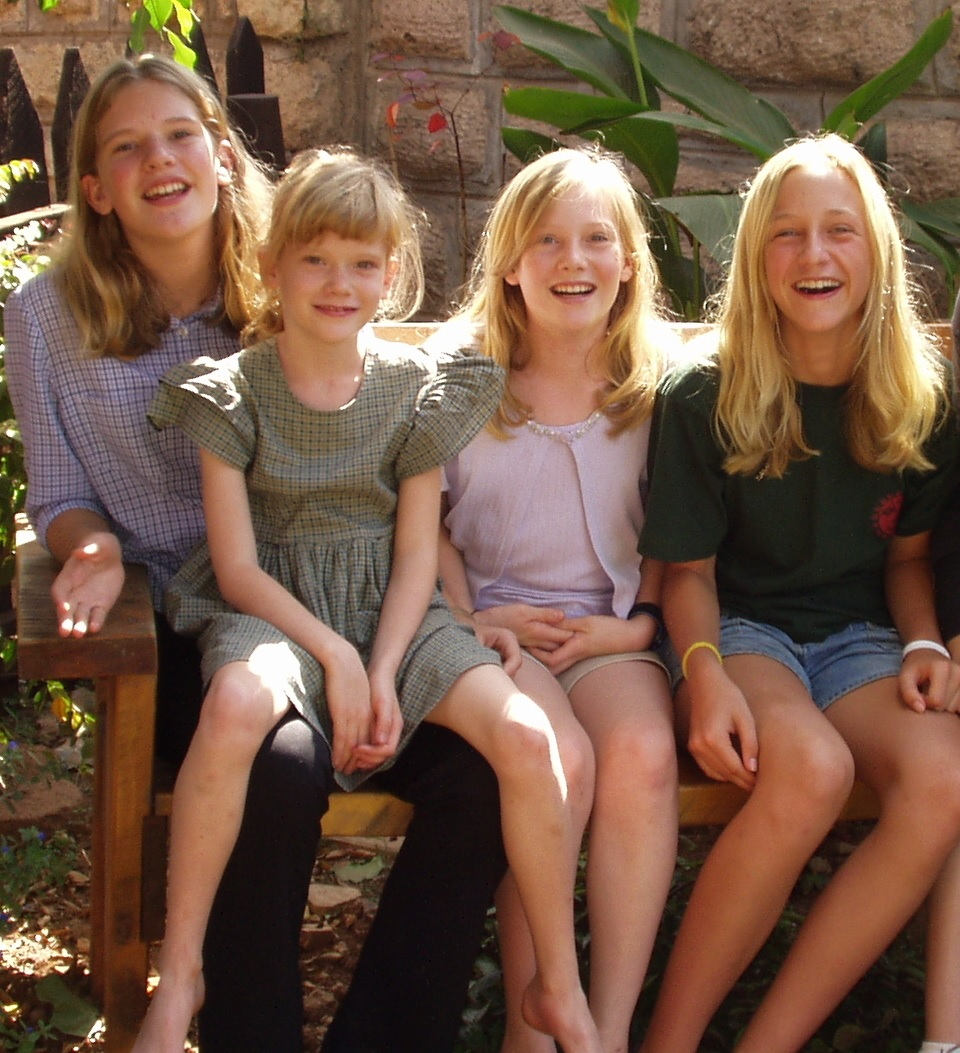
\includegraphics[width=0.75\linewidth]{Girls.jpg}}

%----------------------------------------------------------------------------------------
%	BOOK PART
%----------------------------------------------------------------------------------------

\part{Main}

\chapter{Appetizers}

\begin{minipage}{\linewidth}\rtitle{CHICKEN TARTS} \index{CHICKEN TARTS}
\step{\nicefrac{1}{2} cup butter, softened\\ 
4 oz cream cheese\\ 
1 cup flour\\ 
\nicefrac{1}{2} cup finely chopped chicken \\ 
\nicefrac{1}{2} cup grated Swiss or medium cheddar cheese \\ 
1 large egg \\ 
\nicefrac{1}{2} cup milk\\ 
\nicefrac{1}{4} tsp salt	\\ 
\nicefrac{1}{8} tsp thyme\\ 
\nicefrac{1}{4} tsp onion powder}
{Mix first 3 ingredients for cheese pastry. Shape into long roll. Cut into 24 pieces. Press into tart tins to form shells. Place 1 tsp of chicken in each shell. Process last 6 ingredients in blender until smooth or beat in bowl. Pour into shells. Bake on bottom shelf at 350$^\circ$F for 20 minutes.}

\end{minipage}\par\begin{minipage}{\linewidth}\rtitle{BRIE AND CHERRY PASTRY CUPS} \index{BRIE AND CHERRY PASTRY CUPS}
\step{1 sheet frozen puff pastry	\\ 
\nicefrac{1}{3} to \nicefrac{1}{2} cup red cherry preserves \\ 
2 Tbsp chopped fresh chives	\\ 
\nicefrac{1}{4} cup chopped pecans \\ 
4 oz Brie cheese, cut into $\nicefrac{1}{2} \times \nicefrac{1}{2}$" pcs
}{Heat oven to 375$^\circ$F. Spray 36 miniature muffin cups with cooking spray. Cut pastry into 36 squares. Slightly press each square into muffin cup. Press center with finger. Bake 10 minutes. Press center of each with handle of wooden spoon. Bake 6 to 8 minutes longer or until golden brown. Immediately press again in center. Fill each with about \nicefrac{1}{2} tsp preserves. Top with cheese piece, pecans and chives. Bake 3-5 minutes or until cheese is melted. Serve warm.}

\end{minipage}\par\begin{minipage}{\linewidth}\rtitle{POTATO SKINS (GF)} \index{POTATO SKINS (GF)} \index{Gluten Free!appetizers}
\step{12 new potatoes	\\
2 Tbsp butter, melted \\
1 tsp Dijon mustard	\\
coarse salt \\
\nicefrac{3}{4} cup cheese, grated	\\
8 slices bacon, cooked crisp and crumbled \\
Garnish:  sour cream, sliced onion greens}
{Cut potatoes crosswise into thirds. Use the 2 ends for potato skins and save the middle slices in water for future use. Preheat oven to 425$^\circ$F. Whisk together butter and mustard. Halve each potato piece and hollow out, leave \nicefrac{1}{4} inch shells. Immediately toss the halves in the mustard mixture. Roast, cut side down, on a lightly oiled baking sheet, until nicely browned, 20-30 minutes. Sprinkle with coarse salt. Turn the potatoes upright and cover with grated cheese. Sprinkle with bacon. At this point, potatoes can be held at room temp for up to 2 hours before serving. Return potatoes to oven and bake until hot, about 5 minutes. Garnish with sour cream and onion greens.}

%\end{minipage}\par\begin{minipage}{\linewidth}\rtitle{GORGONZOLA AND HAZELNUT STUFFED MUSHROOMS} \index{GORGONZOLA AND HAZELNUT STUFFED MUSHROOMS}
%\step{1 lb fresh whole mushrooms	\\
			%\nicefrac{1}{3} cup gorgonzola cheese, crumbled \\
			%\nicefrac{1}{4} cup fine bread crumbs	\\
			%\nicefrac{1}{4} cup hazelnuts, chopped \\
			%\nicefrac{1}{4} cup red bell pepper, finely chopped	\\
			%4 med green onions, chopped\\
			%\nicefrac{1}{2} tsp salt}
%{Heat oven to 350$^\circ$F. Remove stems from mushroom caps. Reserve caps. Finely chop enough stems to measure \nicefrac{1}{2} cup. Discard remaining stems. Mix chopped mushroom stems and remaining ingredients in small bowl until well blended. Spoon into mushroom caps, mounding slightly. Place in ungreased pan. Bake 15--20 minutes or until thoroughly heated. Serve warm.}

\end{minipage}\par\begin{minipage}{\linewidth}\rtitle{GINGER CHICKEN AND BACON BITES (GF)} \index{GINGER CHICKEN AND BACON BITES (GF)} \index{Gluten Free!appetizers}
\step{8 oz can whole water chestnuts	\\
\nicefrac{1}{4} cup orange marmalade \\
2 Tbsp soy sauce	\\
\nicefrac{1}{2} tsp ground ginger \\
\nicefrac{1}{8} tsp garlic powder	\\
12 slices bacon \\
12 oz skinless, boneless chicken breasts}
{Cut chicken into 24 bite size pieces. For marinade, combine orange marmalade, soy sauce, ginger and garlic powder in med mixing bowl. Add chicken pieces, tossing to coat. Cover and chill for 30 minutes, stirring occasionally. Meanwhile, arrange bacon slices on unheated rack of broiler pan. Broil 4-5 inches from heat for 1-2 minutes or until partially cooked but not crisp. Drain off fat. Cool bacon and halve slices crosswise. Cut water chestnuts in half crosswise. Drain chicken pieces, discarding marinade. Wrap a piece of bacon around chicken piece and water chestnut half. Secure with wooden toothpick. Place on unheated rack of broiler pan. Broil 4-5" from heat for 3-5 minutes or until check is tender and no longer pink, turning once. Makes 24.}

%\end{minipage}\par\begin{minipage}{\linewidth}\rtitle{CHRISTMAS TREE APPETIZERS} \index{CHRISTMAS TREE APPETIZERS}
%\step{1 pkg cream cheese, softened	\\
	%\nicefrac{1}{2} cup roasted red bell peppers, chopped 	\\
	%\nicefrac{1}{4} cup ripe olives, chopped 	\\
	%\nicefrac{1}{4} cup fresh basil leaves, chopped	\\
	%\nicefrac{1}{4} cup parmesan cheese, shredded		\\
	%4 spinach flavour flour tortillas (8-10-inch)	\\
	%Ripe olive pieces}
%{Mix all ingredients except tortillas and olive pieces. Divide mixture among tortillas, spreading to edges. Roll up tightly. Press each tortilla roll into triangle shape, using fingers. Wrap in plastic wrap. Refrigerate at least 2 hours but no longer than 24 hours.
%To serve, cut rolls into \nicefrac{1}{2}-inch slices. Place olive piece at bottom of each triangle to look like tree trunk. Secure with toothpick.}

\end{minipage}\par\begin{minipage}{\linewidth}\rtitle{BEEF AND SPINACH ROLL-UPS} \index{BEEF AND SPINACH ROLL-UPS}
\step{\nicefrac{1}{4} cup mayonnaise	\\
	\nicefrac{1}{2} tsp garlic powder \\
	2 spinach flavoured tortillas	\\
	1 cup fresh spinach \\
	\nicefrac{1}{4} lb thinly sliced cooked roast beef	\\
	\nicefrac{3}{4} cup shredded cheddar cheese \\
	1 med tomato, chopped}
{Mix mayonnaise and garlic powder in small bowl. Spread mixture evenly over tortillas. Top tortillas with layers of spinach, beef, cheese and tomato. Roll up tightly. Trim ends from rolls. Cut each roll into 12 slices. Secure with toothpicks. Serve immediately or refrigerate until serving.}

\end{minipage}\par\begin{minipage}{\linewidth}\rtitle{MUSHROOM TRIANGLES} \index{MUSHROOM TRIANGLES}
\step{1 \nicefrac{1}{2} cups sliced fresh mushrooms	\\
\nicefrac{1}{4} cup chopped onion\\
1 Tbsp butter	\\
125 g cream cheese, cut up	\\
\nicefrac{1}{4} tsp Worcestershire sauce\\
\nicefrac{1}{4} tsp salt	pepper sprinkle\\
Garlic powder sprinkle
}{Saut\'e until onion is soft and clear. Add remaining ingredients. Stir to melt cheese. Spread on buttered, crustless bread. Fold to make triangles. Press edges. Brush with melted butter. Toast triangles at 400$^\circ$F for about 10--15 minutes.}


%\end{minipage}\par\begin{minipage}{\linewidth}\rtitle{POACHED SALMON APPETIZER (LC*,GF*)} \index{POACHED SALMON APPETIZER (LC*,GF*)} \index{Gluten Free!appetizers} \index{Low Carb!appetizers}
%\step{
%1 lb salmon fillet\\
%4 cups water	\\
%3 or 4 slices lemon, cut in half\\
%3 or 4 slices onion, cut in half\\
%\nicefrac{1}{4} cup small springs parsley\\
%\nicefrac{1}{2} tsp salt \\
%\nicefrac{1}{4} tsp coarsely ground pepper}
%{In 10 or 12" skillet, heat water, lemon and onion slices, parsley, salt and pepper, to boiling. Boil 3 minutes. Reduce heat to med-low. Add salmon, skin side down. Cover and cook 5--6 minutes or until salmon flakes easily with fork. Remove salmon from liquid in skillet. Cool completely. Cover and refrigerate at least 2 hours but no longer than 24 hours. Discard liquid in skillet.}
%
%\step{Sauce:\\
%2 Tbsp lemon juice	\\
%1 Tbsp honey\\
%1 Tbsp Dijon mustard	\\
%1 Tbsp olive or vegetable oil\\
%\nicefrac{1}{4} cup chopped fresh parsley	\\
%2 Tbsp finely chopped red onion\\
%2 tsp capers	\\
%1 tsp grated lemon peel\\
%\nicefrac{1}{4} tsp salt	\\
%cocktail bread slices or crackers, if desired}
%{In small bowl, mix lemon juice, honey, mustard and oil until well blended. In another small bowl, mix chopped parsley, red onion, capers and lemon peel. To serve, carefully remove skin from salmon. Place salmon on serving plate. Sprinkle with \nicefrac{1}{4} tsp salt. Drizzle honey-mustard sauce over salmon; sprinkle with parsley mixture. Serve with bread slices.}


\end{minipage}\par\begin{minipage}{\linewidth}\rtitle{COCKTAIL MEATBALLS} \index{COCKTAIL MEATBALLS}
\step{1 lbs lean ground beef
\\ 1 egg
\\ 2 Tbsp water
\\ \nicefrac{1}{2} cup bread crumbs
\\ 3 Tbsp minced onion
\\ 1 8-oz can jellied cranberry sauce
\\ \nicefrac{3}{4} cup chili sauce
\\ 1 Tbsp brown sugar
\\ 1 \nicefrac{1}{2} tsp lemon juice}{Preheat oven to 350${}^\circ$F. In large bowl, mix beef, egg, water, bread crumbs and onion. Roll into small meatballs. Bake in oven for 20--25 minutes, turning once. In a slow cooker or large saucepan over low heat, blend cranberry sauce, chili sauce, brown sugar and lemon juice. Add meatballs and simmer for 1 hour before serving.}


\end{minipage}\par\begin{minipage}{\linewidth}\rtitle{DEVILS ON HORSEBACK} \index{DEVILS ON HORSEBACK}
\name{The first time I tried these was at the British High Commission in Nairobi.  Daddy and I were part of a 5 voice ensemble that performed a debut work together with a white Kenyan actor and playwright. I don't remember her name but if I remember right the debut work was in celebration of her decades of contributions to the theatre scene in Nairobi. The performance was a farcical look at British history through music and acting. It was all very ``colonial.'' I have a vivid image of the Egyptian ambassador sitting in front of me, sleeping through most of it. The evening must have been a fund-raiser for something medical because our family doctor, Dr. Safwat, was there to give a speech. These traditional British appetizers were served at the reception.} \\
\step{30 pitted prunes \\
10 strips smoked bacon, cut in thirds \\
30 toothpicks}{
Place prune on one end of bacon strip. Roll and secure with toothpick. Place on baking sheet. Bake at 375${}^{\circ}$F until bacon is cooked and crispy, approximately 15--20 min. Flip the appetizers half way through. Serve hot.}

\end{minipage}\par\begin{minipage}{\linewidth}\rtitle{BACON WRAPPED SMOKIES} \index{BACON WRAPPED SMOKIES} 
\name{(Kelly Penner)}\\
\step{1 lb bacon, sliced in thirds \\
14 oz pkg beef cocktail weiners \\
\nicefrac{3}{4} cup brown sugar (or more if needed)}{
Sprinkle sugar on bacon strips. Wrap cocktail wiener in strip of bacon. Place wrapped wieners on foil-lined baking sheet. Sprinkle with sugar. Bake at 325${}^{\circ}$F for 25 min. Raise temperature to 350${}^{\circ}$F for last 15 min of baking. }


%\end{minipage}\par\begin{minipage}{\linewidth}\rtitle{WINGS PARMESAN} \index{WINGS PARMESAN}
%\name{(Company's Coming)} \\
	%\step{\nicefrac{3}{4} cup Grated parmesan cheese	 \\
	 %\nicefrac{1}{4} cup fine dry bread crumbs \\
	 %1 tsp paprika \\	
	 %1 tsp salt \\
	 %\nicefrac{1}{4} tsp pepper	 \\
	 %\nicefrac{1}{4} tsp oregano \\
	 %\nicefrac{1}{4} tsp thyme	 \\
	 %\nicefrac{1}{2} cup melted butter \\
	 %900 g chicken wings}{Mix first 7 ingredients together. Cut off chicken wing tips and discard. Dip wings into melted butter then coat with dry mixture. Arrange on greased, foil lined baking sheet. Bake in 350$^\circ$F oven for 30--45 minutes until tender.}

\end{minipage}\par\begin{minipage}{\linewidth}\rtitle{BARBECUE SAUCED WINGS (GF)} \index{BARBECUE SAUCED WINGS (GF)} \index{Gluten Free!appetizers} 
\step{1 kg chicken wings	\\
\nicefrac{1}{4} cup ketchup\\
\nicefrac{1}{4} cup water	\\
\nicefrac{1}{4} cup brown sugar, packed	\\
\nicefrac{1}{4} cup vinegar	\\
2 Tbsp Worcestershire sauce	\\
2 Tbsp cooking oil	\\
1 tsp prepared mustard\\	
1 tsp paprika	\\
1 tsp salt	\\
\nicefrac{1}{4} tsp pepper	\\
1 Tbsp dry onion flakes\\
}
{}

\end{minipage}\par\begin{minipage}{\linewidth}\rtitle{TERIYAKI CHICKEN WINGS (LC*,GF*)} \index{TERIYAKI CHICKEN WINGS (LC*,GF*)} \index{Gluten Free!appetizers}
\step{1.35 kg chicken wings\\
\nicefrac{1}{2} cup soy sauce	\\
\nicefrac{1}{2} cup sake (or apple juice)\\
3 Tbsp sugar	\\
1 garlic clove minced\\
\nicefrac{1}{4} tsp ginger	\\
\nicefrac{1}{2} tsp paprika \\
\nicefrac{1}{2} tsp chili powder}
{Remove chicken wing tips and discard. Arrange in greased pan large enough to hold in single layer. Mix remaining 7 ingredients together. Spoon over chicken. Bake uncovered in 350$^\circ$F oven for 30-45 minutes until tender.}

\end{minipage}\par\begin{minipage}{\linewidth}\rtitle{BOURBON CIDER BONELESS WINGS} \index{BOURBON CIDER BONELESS WINGS}
\step{SAUCE: \\
12 oz apple cider or apple juice concentrate, thawed \\
1 cup bourbon \\
\nicefrac{1}{2} cup soy sauce \\
\nicefrac{1}{4} cup apple cider vinegar \\
\nicefrac{1}{4} cup brown sugar \\
5 cloves garlic, grated finely \\
1 Tbsp maple syrup \\
1 tsp salt \\
\nicefrac{1}{4} tsp red pepper flakes \\
\nicefrac{1}{4} tsp cayenne pepper}{Add all ingredients to saucepan and bring to a boil over high heat. Reduce to low and simmer for 35 minutes, until sauce has reduced and chickened. Set aside to cool.}

\step{2 lbs chicken breasts, diced into \nicefrac{1}{2}--1" pieces \\
2 cups buttermilk \\
Salt and pepper \\
1 tsp dried thyme \\
2 cups flour \\
\nicefrac{1}{3} cup panko breadcrumbs \\
\nicefrac{2}{3} Tbsp buttermilk \\
Oil for frying}{Sprinkle diced chicken with salt, pepper and thyme. Cover with buttermilk and stir until chicken is well-coated. Cover and refrigerate for 30 minutes. Heat oil in large pot. Add flour, panko, salt and pepper to a large ziplock bag. Shake to combine. Add in 2--3 Tbsp buttermilk and stir until breading mixture is clumpy. Use slotted spoon to transfer chicken into plastic bag. Seal bag and toss to coat chicken. Add chicken, about 8 pieces at a time, to hot oil and fry 4--5 minutes, flipping halfway through. Cool chicken on wire cooling rack. Toss fried chicken with sauce.  Optional: Place glazed chicken on a parchment paper lined baking sheet and broil 2--3 minutes until extra sticky.}


\end{minipage}\par\begin{minipage}{\linewidth}\rtitle{QUESADILLAS} \index{QUESADILLAS}
	\step
	{125 g cream cheese, softened	 \\
	 \nicefrac{1}{3} cup salsa, medium \\
	 \nicefrac{1}{3} cup chopped green pepper \\	
	 1 large tomato, seeded and diced \\
	 3 green onions, chopped	 \\
	 6 flour tortillas \\
	 114 ml canned chopped green chillies, drained \\
	 375 ml (1 \nicefrac{1}{2} cups) grated Monterey Jack cheese \\
 Guacamole, salsa and sour cream for dipping}{Mash cream cheese and salsa together with fork. Set aside. Toss next 4 ingredients in bowl. Spread \nicefrac{1}{2} of each tortilla with cream cheese mixture to \nicefrac{1}{2} inches from edge. Sprinkle green pepper mixture over cream cheese mixture. Sprinkle each with grated cheese. Fold uncovered half over filling. Press edges lightly with your hand. Arrange on ungreased baking sheet. Bake in 425$^\circ$F oven for 10--15 minutes or toast under broiler. Cut into 4 wedges each. Serve with dipping sauces.}

\end{minipage}\par\begin{minipage}{\linewidth}\rtitle{JAMAICAN ROTI} \index{JAMAICAN ROTI}
\name{(Yvonne Hiebert)} \\
  \step{PASTRY: \\
	 2 cup flour	\\
	 1\nicefrac{1}{2} tsp baking powder	\\
	 1 tsp curry		\\
	 \nicefrac{1}{2} tsp salt	\\
	 \nicefrac{2}{3} cup shortening		\\
	 \nicefrac{1}{4} cup butter	\\
	 \nicefrac{1}{3}--\nicefrac{1}{2} cup water	
	\stepspace  MEAT FILLING: \\
	 1 small onion \\
	 3 green onions \\
	 2 cloves garlic \\
	 2 tsp oil. \\
   1 lb ground beef, browned	 \\
	 pinch cayenne pepper \\
	 1 tsp thyme	 \\
	 \nicefrac{1}{2} tsp salt and pepper \\
	 \nicefrac{2}{3} cup water \\
	 1 cup fresh bread crumbs}{Mix pastry ingredients as for pie dough. Roll out and cut rounds with a cup. Fill with meat filling and fold over. Brush edges with water to help stick together. Press edges together with a fork and pierce top twice. Bake 20 minutes at 375$^\circ$F. For meat filling, saute onions and garlic in toil. Add beef and brown. Add spices and water and bring to boil. Add bread crumbs. Let cool.}

\end{minipage}\par\begin{minipage}{\linewidth}\rtitle{MEAT PRIZHKY} \index{MEAT PYROHY} \index{MEAT PRIZHKY}
\name{(Loraine Hiebert)} \\
\step{1 pkg. yeast	
	\\ 1 tsp sugar
	\\ \nicefrac{1}{2} cup water
	\\ 1 cup milk, scalded
	\\ 1 tsp sugar	
	\\ \nicefrac{1}{2} cup warm water
	\\ \nicefrac{1}{3} cup oil	
	\\ 2 eggs, beaten
	\\ 1 TBSP salt	
	\\ 2 \nicefrac{1}{2} cups flour
	\\ 2 \nicefrac{1}{2} cups flour}{
Dissolve yeast and sugar in water. Let stand 10 minutes and add yeast to rest of ingredients, except final flour.
Beat thoroughly and gradually add final 2 \nicefrac{1}{2} cups more of flour. Knead well. Cover. Let stand in warm place to rise until double in bulk. (1 hour or so). Roll out. Place filling on dough. I use cookie cutter to make my pyrohy. Let rise. Bake at 350$^\circ$F for 25 minutes. Makes 4-5 doz. Serve with sour cream.}

\step{FILLING:
	\\ 1 med. onion, chopping fine	
	\\ 4 Tbsp butter
	\\ 1 lb. ground beef or half pork/half beef
	\\ 1 tsp salt 
	\\ pepper	
	\\ 1 Tbsp flour
	\\ \nicefrac{1}{2} cup soup stock of water	
	\\ 1 tsp chopped parsley
	\\ 2 hard cooked eggs, chopped}{
Cook onions in half the butter until tender. Add remaining butter (Mom doesn't) and meat. Brown meat lightly. Season with salt and pepper. Cover and cook over low heat until done. Remove meat. Stir flour into drippings. Add soup stock then cook, stirring until sauce comes to boil. Combine with meat. Cool. Mix in parsley and chopped eggs.}

\end{minipage}\par\begin{minipage}{\linewidth}\rtitle{OLIVE CHEESE BALLS} \index{OLIVE CHEESE BALLS}
\name{(Jeanie Little)} \\
\step
	{2 cup sharp cheddar cheese, grated \\
 1 cup flour \\
 \nicefrac{1}{2} cup butter \\
 1--2 tsp chili powder \\
 48 stuffed olives}{Blend cheese with butter. Add dry ingredients. Mix well. Wrap about 1 tsp of this mixture around olive, covering completely. (This is the tricky bit and can take a bit of patience! I flatten the dough in the palm of my hand and then wrap it. It also helps if the olives are drained well.) Bake at 400$^\circ$F for 15 minutes on a cookie sheet.}


%\end{minipage}\par\begin{minipage}{\linewidth}\rtitle{JALAPENO BACON DEVILED EGGS (GF)} \index{JALAPENO BACON DEVILED EGGS (GF)} \index{Gluten Free!appetizers}
	%\step
	%{12 large eggs, hard-boiled and peeled\\
	 %paprika\\
	 %1.5 tsp rice vinegar	\\
	 %\nicefrac{3}{4} tsp ground mustard \\
	 %2 jalapenos, seeded and chopped	\\
	 %6 pieces bacon, cooked, crumbled
		%}{}
		
\end{minipage}\par\begin{minipage}{\linewidth}\rtitle{CRAB PURSES} \index{CRAB PURSES}
\name{A little fussy but very elegant looking. Can be steamed up to an hour ahead then resteamed to heat them just before serving.} \\
	\step
	{24 green onion tops, cut into 3-inch julienne pieces	 \\
	 6 oz lump crabmeat	 \\
	 1  4-oz block cream cheese \\	
	 \nicefrac{1}{4} cup minced green onions	 \\
	 2 tsp fresh lemon juice \\
	 \nicefrac{1}{2} tsp hot sauce	 \\
	 \nicefrac{1}{4} tsp salt \\
	 \nicefrac{1}{8} tsp pepper	 \\
	 24 won ton wrappers \\
	 1 egg white, lightly beaten	 \\
	 2 Tbsp soy sauce \\
	 1 Tbsp water	 \\
	 1 Tbsp fresh lemon juice	
		}{
Drop green onion strips in boiling water and cook 10 sec or until limp. Drain and set aside. Combine crabmeat and next 6 ingredients in a medium bowl and stir well. Working with 1 won ton wrapper at a time, cover remaining wrappers with a damp towel, spoon 2 tsp mixture into center of wrapper. Moisten edges of wrapper with egg white. Gather 4 corners of wrapper and crimp to seal, forming a purse. Tie 1 green onion strip around crimped top of purse (like a child's drawstring purse). Repeat with remaining won tons wrappers. Arrange half of won ton purses in a single layer in a vegetable steamer coated with cooking spray. Steam purses, covered, 8 minutes or until tender. Carefully remove purses from steamer; set aside and keep warm. Repeat with remaining purses. Combine soy sauce, water and 1 Tbsp lemon juice in a small bowl. Stir well. Serve with purses.}

\end{minipage}\par\begin{minipage}{\linewidth}\rtitle{CRAB SALAD (GF)} \index{CRAB SALAD (GF)} \index{Gluten Free!appetizers}
\name{Ideal as salad or as filling for Pita sandwiches.}\\
\step{8--10 oz. sea legs (fake crab)
\\	\nicefrac{1}{2} cup mayonnaise	
\\	\nicefrac{1}{4} cup sour cream
\\	\nicefrac{1}{4} cup chopped green onion	
\\	\nicefrac{1}{4} cup chopped cucumber or celery
\\	1 hard cooked egg, chopped	
\\	1 Tbsp lemon juice
\\	2 tsp chopped fresh or dried dill weed	
\\	\nicefrac{1}{8} tsp pepper}{Pull sea legs apart into small pieces. Remove seeds from cucumbers. Assemble.}

\end{minipage}\par\begin{minipage}{\linewidth}\rtitle{MANGOS WITH SPICY PRAWNS (GF)} \index{MANGOS WITH SPICY PRAWNS (GF)} \index{Gluten Free!appetizers}
\step{3 cups uncooked prawns \\
2 whole mangoes\\
juice of 1 lemon\\
2 Tbsp ketchup	\\
3 cups whipped cream\\
\nicefrac{1}{2} cup chopped apple	\\
1 Tbsp horseradish\\
parsley and lemon for garnish\\
}
{Cut the mangoes into halves and remove stone. Drop prawns into boiling salted water with juice of one lemon and boil for five minutes. Remove the prawns, cool and peel. Mix the prawns with the cocktail sauce (ketchup, whipped cream, apple, and horseradish) and place them in the center of each mango half. Garnish with parsley and lemon wedges. Serves 4.}

\end{minipage}\par\begin{minipage}{\linewidth}\rtitle{HERBED BRUSCHETTA} \index{HERBED BRUSCHETTA}
Yield: 32 slices \\
	\step
	{8 fresh ripe plum tomatoes, very finely diced \\
	 2 Tbsp finely minced garlic	\\
	 \nicefrac{1}{2} cup coarsely chopped fresh basil\\
	 Pinch crushed red pepper flakes	\\
	 salt and pepper\\
	 32 \nicefrac{1}{4}-inch thick slices French baguette	\\
	 6 garlic cloves, cut in half
		}{
Combine tomato, minced garlic, basil, parsley, lemon juice, red pepper, salt and pepper. Toss and set aside for at least 3 hours. Just before serving, toast the bread and rub on one side with cut sides of garlic cloves. Place a small bowl in center of serving platter. Fill bowl with tomato mixture and arrange toast around the bowl. }

\end{minipage}\par\begin{minipage}{\linewidth}\rtitle{SURPRISE SPREAD (LC,GF)} \index{SURPRISE SPREAD (LC,GF)} \index{Gluten Free!appetizers}
	\step
	{8 oz. cream cheese	\\
	 \nicefrac{1}{2} cup sour cream\\
	 \nicefrac{1}{4} cup mayonnaise	\\
	 1 or 2 cans small or broken shrimp\\
	 1 cup seafood cocktail sauce (or \nicefrac{1}{2} cup ketchup \& \nicefrac{1}{2} cup horseradish) \\
	 2 cups shredded mozzarella cheese	\\
	 1 green pepper\\
	 3 green onions	\\
	 1 tomato, diced}{Mix first 3 ingredients. Spread in pizza pan and layer next 6 ingredients in order given. Cover and chill. Serve with crackers.}

\end{minipage}\par\begin{minipage}{\linewidth}\rtitle{CRAB CHEESE DIP (GF)} \index{CRAB CHEESE DIP (GF)} \index{Gluten Free!appetizers}
	\step
	{\nicefrac{1}{2} cup mayonnaise	\\
	 1 8-oz pkg cream cheese\\
	 2 Tbsp milk	\\
	 4 scallions, sliced\\
	 1 Tbsp lemon juice	\\
	 1 tsp red pepper sauce\\
	 1 tsp Worcestershire sauce	\\
	 \nicefrac{1}{2} tsp garlic salt\\
	 \nicefrac{1}{2} cup grated parmesan cheese	\\
	 1 lb lump crab meat\\
	 \nicefrac{1}{4} cup parsley, chopped\\
		}{
Spray 6 cup shallow baking dish (quiche dish). Combine first 8 ingredients plus \nicefrac{1}{4} cup parmesan cheese. Gently stir in crab meat. Sprinkle remaining \nicefrac{1}{4} cup cheese over top. Bake 30 minutes at 350${}^\circ$F. Sprinkle with parsley. Serve warm with tortilla chips.}

\end{minipage}\par\begin{minipage}{\linewidth}\rtitle{BAKED SPINACH DIP} \index{BAKED SPINACH DIP}
\name{(Priscilla Koehler)}\\
\step{8 oz cream cheese, softened
\\ \nicefrac{1}{2} cup mayonnaise
\\ 2 cloves garlic, minced or pressed
\\ \nicefrac{1}{2} cup freshly grated parmigiano reggiano (parmesan cheese)
\\ \nicefrac{1}{2} cup shredded asiago cheese
\\ 1 tsp onion powder
\\ \nicefrac{1}{4} tsp salt
\\ \nicefrac{1}{4} tsp black pepper
\\ 1 10-oz. pack of chopped frozen spinach (thawed and drained)}{Preheat oven to 350${}^\circ$F. Combine all ingredients, except the spinach, and mix until well blended. Add spinach. Pour mixture into a small casserole dish. Sprinkle some shredded asiago cheese on top. Bake for 30 minutes.}

\end{minipage}\par\begin{minipage}{\linewidth}\rtitle{SPINACH DIP IN PUMPERNICKEL BREAD} \index{SPINACH DIP IN PUMPERNICKEL BREAD}
	\step
	{1 pkg. frozen chopped spinach (thaw and drain well, wring out moisture)\\
	 1 pkg. vegetable soup mix\\	
	 1 onion green, chopped\\
	 1 cup sour cream	\\
	 1 cup mayonnaise \\
	 1 8-oz. can water chestnuts	\\
	 1 loaf pumpernickel bread \\
	opt:\\
	rosemary sprigs\\
	fresh spinach leaves\\
	cherry tomatoes
		}{
Combine ingredients. Cut and hollow out 3-inch wide rim on top of bread to within \nicefrac{1}{2}-inch of bottom, leave center of loaf intact. Reserve scooped out bread. Spoon spinach dip into hollowed out ring. Tear reserved bread into bite size pieces. Use bread for dipping. Garnish tip:  Make a wreath of rosemary sprigs and fresh spinach leaves around the base of the bread bowl. Add cherry tomatoes to represent berries in the wreath.}

\end{minipage}\par\begin{minipage}{\linewidth}\rtitle{CAMEMBERT AND PUMPERNICKEL BREAD} \index{CAMEMBERT AND PUMPERNICKEL BREAD}
I got this idea from Sabine, my German neighbour in Matumbatu Estates \#25. We shared equal passions for cooking and gardening. Sometimes Sabine would give me a jar of her homemade tree tomato jam, which went along perfectly with this dish.
Hollow out a pumpernickel bread (or other round bread). Reserve bread for dipping. Place a round of camembert into the bread round. Place bread round on cookie sheet and heat in oven (350$^\circ$F) until cheese is soft.

\end{minipage}\par\begin{minipage}{\linewidth}\rtitle{SNOWBALL DIP WITH FRENCH BREAD} \index{SNOWBALL DIP WITH FRENCH BREAD}
\name{(Robert Derosiers	from Southern Health)}\\
\step{2 pkgs cream cheese
\\ 1 cup mayonnaise
\\ \nicefrac{1}{2} cup green onions, chopped
\\ 1 cup old cheddar cheese, grated
\\ \nicefrac{1}{2} cup bacon bits
\\ 1 tsp dill
\\ Garlic salt to taste
\\ 3 generous dashes Worcestershire
\\ 3 dashes of tabasco
\\ 1 heaping tsp Dijon mustard
\\ 2 loaves of French bread (not baguettes)}{Cut top of one loaf of bread and hollow it out.  Use the pieces of bread for dipping. Cut up the other loaf for dipping as well. Combine dip ingredients.  Fill hollowed out loaf. Wrap in foil. Put in oven at 350${}^\circ$F for 45--60 minutes.}

\end{minipage}\par\begin{minipage}{\linewidth}\rtitle{MEXICAN FIESTA DIP (GF)} \index{MEXICAN FIESTA DIP (GF)} \index{Gluten Free!appetizers}
	\step
	{8 oz container sour cream		\\
	 1 envelope taco seasoning mix	\\
	 16 oz can refried beans		\\
	 \nicefrac{1}{2} cup pickled jalapeno peppers, sliced	\\
	 4 oz (1 cup) cheddar cheese, shredded		\\
	 1 \nicefrac{1}{2} cups lettuce, shredded	\\
	 1 large tomato, chopped}
	{Combine sour cream and taco seasoning mix. Spread refried beans onto a 9-inch round serving plate; spoon sour cream mixture evenly over beans. Layer with jalapeno peppers and the next 4 ingredients. Serve with tortilla chips.
}

\end{minipage}\par\begin{minipage}{\linewidth}\rtitle{CILANTRO BLACK BEAN DIP (GF)} \index{CILANTRO BLACK BEAN DIP (GF)} \index{Gluten Free!appetizers}
	\step
	{1 540 mL can of black beans, drained \& rinsed \\
	 \nicefrac{2}{3} cup packed, chopped cilantro (leaves \& stems)	\\
	 3 cloves garlic, crushed		\\
	 2 Tbsp lime juice	\\
	 1 Tbsp tomato paste		\\
	 1 Tbsp olive oil	\\
	 1 tsp sea salt		\\
	 \nicefrac{1}{2} tsp cayenne pepper or chipotle chili powder \\
   \nicefrac{1}{2} tsp ground coriander \\
   \nicefrac{1}{2} tsp cumin \\
   \nicefrac{1}{4} cup water to thin dip as desired}{Blend in food processor or blender.}

\end{minipage}\par\begin{minipage}{\linewidth}\rtitle{CHILI DIP (GF*)} \index{CHILI DIP (GF*)} \index{Gluten Free!appetizers} 
\name{(Erma Penner)}\\
	\step{250 g cream cheese		\\
	 1 cup sour cream	\\
	 1 28 oz can mild chilli or use homemade chilli	\\
	 1 cup salsa	\\
	 shredded cheddar cheese
		}{Mix cream cheese and sour cream together. Spoon chilli on top of this. Pour salsa on top. Bake at 400$^\circ$F for 20 minutes. Cover with shredded cheese and bake 5 more minutes. Serve hot with taco chips.}
		
\end{minipage}\par\begin{minipage}{\linewidth}\rtitle{GUACAMOLE (GF)} \index{GUACAMOLE (GF)} \index{Gluten Free!appetizers} 
\step{4 avocados
\\ 1 tomato
\\ \nicefrac{1}{2} onion
\\ 1 jalape\~no
\\ small bunch of cilantro
\\ 1-2 garlic cloves
\\ fresh juice of 1--2 limes
\\ salt to taste}{Mash avocados. Finely chop tomato, onion, and jalape\~no. Add all ingredients.}

\end{minipage}\par\begin{minipage}{\linewidth}\rtitle{VEGETABLE DIP (GF)} \index{VEGETABLE DIP (GF)} \index{Gluten Free!appetizers}
\step{1 cup mayonnaise	\\
\nicefrac{1}{2} cup sour cream \\
1 Tbsp onion	\\
\nicefrac{1}{4} tsp paprika \\
1 Tbsp chives	 \\
\nicefrac{1}{8} tsp curry powder \\
1 tsp garlic salt	\\
\nicefrac{1}{2} tsp Worcestershire sauce}
{}

\end{minipage}\par\begin{minipage}{\linewidth}\rtitle{TACO DIP (GF)} \index{TACO DIP (GF)} \index{Gluten Free!appetizers} 
\name{Makes a nice change from salsa with taco chips.}\\
\step{1 cup mayonnaise \\
1 cup sour cream \\
1 pkg. taco spices}{}

\end{minipage}

\chapter{Main Meals}

\section{Beef}

\begin{minipage}{\linewidth}\rtitle{SWISS "STINK" STEAK} \index{SWISS "STINK" STEAK}
\textit{(Moira Neufeld)}\\
\step{steak (round or chuck), cut into 2--3" pieces \\
onions, slices\\
carrots, chopped\\
parsnips, chopped\\
celery and leaves, chopped\\
1 can tomato soup	\\
2 Tbsp Worcestershire sauce\\
1 Tbsp brown sugar	\\
\nicefrac{2}{3} tsp dry mustard\\
1 clove garlic	\\
oregano\\
1 bay leaf\\
Salt and pepper \\
strong cheddar, grated}{Brown steak well in oil in heavy skillet. Salt and pepper while browning. Place in baking dish and cover with onions, carrots, parsnips, and celery. Mix remaining ingredients except cheese and add to vegetables and steak. Cover with tin foil. Bake in 400$^\circ$F oven for 2--3 hours. Optional: last 5 minutes, remove cover and sprinkle with grated strong cheddar.}

\end{minipage}\par\begin{minipage}{\linewidth}\rtitle{ROUND STEAK SAUERBRATEN} \index{ROUND STEAK SAUERBRATEN}
\step{1\nicefrac{1}{2} lb. round steak	\\
1 envelope brown gravy mix (or 2 	bouillon cubes and 2 Tbsp cornstarch) \\
1 Tbsp minced onion	\\
1 Tbsp brown sugar\\
2 Tbsp wine sugar	\\
1 tsp Worcestershire sauce\\
\nicefrac{1}{4} tsp ginger	\\
1 bay leaf
}{Cut meat in 1" squares. Brown in 1 Tbsp shortening. Remove from skillet. Add gravy mix, 2 cups water. Bring to boil. Stir in next six ingredients plus \nicefrac{1}{2} tsp salt and pepper. Add meat. Turn into casserole. Cover. Bake 350$^\circ$F for 1\nicefrac{1}{2} hours. Serve on hot buttered noodles.}

\end{minipage}\par\begin{minipage}{\linewidth}\rtitle{HUNGARIAN GOULASH} \index{HUNGARIAN GOULASH}
\step{3 lbs chuck steak
\\ 2 Tbsp butter
\\ 1 \nicefrac{1}{2} litres water or stock
\\ 1 large onion, chopped
\\ 1 bay leaf
\\ 1 tsp salt
\\ Dash of cayenne pepper
\\ 6 med potatoes
\\ 1 tsp paprika
\\ 3 Tbsp flour
\\ 3 Tbsp butter}{Cut meat in cubes, brown quickly in butter, then add the onion and brown slightly. Add stock or water, bay leaf, cayenne, paprika and salt. Simmer 2 \nicefrac{1}{2} hrs. Add potatoes and cook about \nicefrac{1}{2} hr, reducing liquid to approx. 3 cups. Thicken with butter and flour.}

\end{minipage}\par\begin{minipage}{\linewidth}\rtitle{BEEF STROGANOFF} \index{BEEF STROGANOFF}
\step{2 lbs beef chuck roast
\\ \nicefrac{1}{2} tsp salt
\\ 1 tsp prepared mustard
\\ \nicefrac{1}{2} tsp black pepper
\\ 4 oz butter
\\ 4 green onions, white parts only (sliced)
\\ 4 Tbsp flour
\\ 1 10.5 oz can condensed beef broth
\\ 1 cup sliced mushrooms
\\ \nicefrac{1}{3} cup sour cream
\\ \nicefrac{1}{3} cup white wine}{Remove any fat and gristle from the roast and cut into strips \nicefrac{1}{2}" long. Season with \nicefrac{1}{2} tsp salt and \nicefrac{1}{2} tsp pepper. In a large skillet, over med heat, melt butter and brown beef strips quickly. Push beef off to one side. Add onions and mushrooms and cook slowly for 3-5 min, then push to the side with the beef strips. Stir flour into the juice. Pour in beef broth and bring to a boil, stirring constantly. Lower the heat and stir in mustard. Cover and simmer for 1 hr or until meat is tender. Five minutes before serving, stir in the sour cream and white wine. Heat briefly then salt and pepper to taste.  Serve over noodles or rice.}

\end{minipage}\par\begin{minipage}{\linewidth}\rtitle{BEEF BOURGUIGNON} \index{BEEF BOURGUIGNON}
\textit{(Company's Coming)}\\
\step{
	2 lbs boneless lean beef	\\
	2 Tbsp butter\\
	2 Tbsp cooking oil	\\
	225 grams small fresh mushrooms\\
	\nicefrac{1}{4} cup flour	\\
	\nicefrac{1}{2} tsp salt\\
	\nicefrac{1}{2} tsp pepper\\	
	2 cups Burgundy (or alcohol free red wine)\\
	1 clove garlic, minced	\\
	1 bay leaf\\
	1 Tbsp ketchup	\\
	1 tsp parsley flakes\\
	\nicefrac{1}{2} tsp thyme	\\
	3 beef bouillon cubes\\
	1 cup boiling water	\\
	398 ml canned small onions, drained}{
Cut beef into 1 inch cubes. Brown in butter and cooking oil. Transfer to large saucepan when browned. Saut\'e mushrooms for 3-4 minutes. Add to meat in saucepan. Put flour, salt and pepper into frying pan. Add enough butter to moisten flour if needed. Stir in burgundy, garlic, bay leaf, ketchup, parsley and thyme until it boils and thickens. Dissolve beef cubes in boiling water. Add to wine mixture. Stir. Pour over meat. Cover. Simmer for 1 hour. Add onions. Simmer, covered for about 30 minutes more until tender. Discard bay leaf.
Note: 1 \nicefrac{1}{2} cups cooked whole pearl onions or cut up onions, cooked may be substituted for canned onions.}

\end{minipage}\par\begin{minipage}{\linewidth}\rtitle{MARINATED ROAST BEEF} \index{MARINATED ROAST BEEF}
\textit{(Ruth Stalder)}\\
\step{dry mustard	\\
soy sauce \\
	lots of garlic	\\
	herbes de province \\
	red wine
}{Marinate beef for 2 days. Cook in an open roaster for 45 minutes. Baste frequently with the marinade sauce.}

\end{minipage}\par\begin{minipage}{\linewidth}\rtitle{UMAMI ROAST BEEF} \index{UMAMI ROAST BEEF}
\textit{Great pressure cooker recipe}\\
\step{1-3 lb roast
\\ 1 Tbsp olive oil
\\ 2 small onions, sliced
\\ 4 cloves of garlic
\\ 8 white mushrooms
\\ 2 Tbsp of wine or balsamic vinegar
\\ 1 cup chicken stock
\\ 1 Tbsp soy sauce
\\ 1 Tbsp fish sauce
\\ pinch of rosemary
\\ pinch of thyme
\\ 2 bay leaves
\\ 2 carrots, chopped
\\ 2-4 potatoes, quartered
\\ 1.5 Tbsp cornstarch
\\ 2 Tbsp water}{Heat pressure cooker on high with Saute button. Pat roast dry, season generously with salt and pepper, and brown roast for 10 minutes on each side. Remove roast. Add oil and saute onions. Add garlic. Add mushrooms. Add wine or balsamic vinegar to deglaze. Add chicken stock, soy sauce, fish sauce, rosemary, thyme, and bay leaves. Place roast back into pot, close lid, and pressure cook on high pressure for 45 minutes. Turn off heat and let it naturally release for 25 minutes. Remove roast and cover with aluminum foil. Add vegetables to pot and cook at high pressure for 4 minutes. Release pressure. Adjust seasonings and mix cornstarch with water and mix with sauce to make a gravy.}

\end{minipage}\par\begin{minipage}{\linewidth}\rtitle{HOMESTYLE STEW} \index{HOMESTYLE STEW}
\textit{(Company's Coming)}\\
\step{
	1 kg stew meat, cut up	\\
	3 Tbsp cooking oil\\
	4 cups water	\\
	2 med onions, cut up\\
	1 Tbsp Worcestershire sauce	\\
	\nicefrac{1}{2} cup ketchup\\
	1 tsp salt	\\
	1 tsp basil\\
	2 cups sliced carrots	\\
	3 cups potatoes, cup up\\
	1 cup frozen peas}{
Brown meat in cooking oil. Add remaining ingredients, except vegetables. Cover and simmer about 1 \nicefrac{1}{2} hours. Add vegetables. Boil until tender. If desired, gravy may be thickened. Mix 1 Tbsp flour with 2 Tbsp water for each cup of juice.}

\end{minipage}\par\begin{minipage}{\linewidth}\rtitle{WIENER SCHNITZEL} \index{WIENER SCHNITZEL}
\textit{(Company's Coming)}\\
\step{
	1 \nicefrac{1}{2} lbs veal cutlets\\
	\nicefrac{1}{4} cup flour	\\
	1 tsp salt\\
	\nicefrac{1}{4} tsp pepper	\\
	2 eggs\\
	1 Tbsp water	\\
	1 cup fine dry bread crumbs\\
	2 Tbsp margarine	\\
	2 Tbsp cooking oil}{
Place cutlets between sheets of waxed paper. Pound thin. Repeat. Mix flour with salt and pepper. Beat eggs with water to make a wash. Dip cutlets into flour mixture, then into egg wash, then into crumb mixture to coat well. These may be chilled at this point until ready to cook. Heat margarine and cooking oil in frying pan. Cook cutlets browning on both sides turning with puncturing. Add more margarine and cooking oil if needed. Serves 4.}

\end{minipage}\par\begin{minipage}{\linewidth}\rtitle{BEEF PARMIGIANA} \index{BEEF PARMIGIANA}
\textit{(Company's Coming)}\\
\step{
	1 \nicefrac{1}{2} lbs thinly cut round steak\\
	\nicefrac{1}{3} cup fine dry bread crumbs	\\
	\nicefrac{1}{3} cup grated parmesan cheese\\
	1 egg, fork beaten	\\
	\nicefrac{1}{3} cup cooking oil\\
	1 cup chopped onion	\\
	156 ml tomato paste\\
	2 cups water\\	
	1 tsp salt\\
	\nicefrac{1}{4} tsp pepper	\\
	\nicefrac{1}{2} tsp oregano\\
	1 tsp sugar	\\
	225 g mozzarella cheese slices}{
Cut steak into serving size pieces. Place each piece between waxed paper on bread board. Pound with meat mallet to \nicefrac{1}{4} in. thickness. Mix crumbs and cheese together. Dip meat into egg then into crumb mixture. Fry in cooking oil to brown both sides. Transfer to greased $9\times13$" baking pan. Saut\'e onion in pan until soft. Add more oil if necessary. Add tomato paste, water, salt, pepper, oregano and sugar. Stir. Pour over meat. Layer cheese over top. Cover. Bake in 350$^\circ$F oven until tender, about 1 \nicefrac{1}{4} to 1 \nicefrac{1}{2} hours. Serves 4.}

\end{minipage}\par\begin{minipage}{\linewidth}\rtitle{PERFECT GRILLED HAMBURGERS} \index{PERFECT GRILLED HAMBURGERS}
\step{1 lb ground beef (reg ground beef is just fine)
\\ 2 cloves garlic
\\ 1 tsp black pepper
\\ 1 \nicefrac{1}{2} tsp salt
\\ \nicefrac{1}{2} tsp basil
\\ 2 Tbsp olive oil}{Combine all ingredients.  Shape mixture into 4 patties. Grill on BBQ set at high heat for a few minutes on each side.}

\end{minipage}\par\begin{minipage}{\linewidth}\rtitle{BEEF TACO CASSEROLE} \index{BEEF TACO CASSEROLE}
\textit{(Merle Fingas)\\
Loren's favourite childhood casserole.}\\
\step{1 lb. ground beef	
	\\ 2 tsp chilli powder
	\\ 1 med. onion, chopped	
	\\ \nicefrac{1}{2} tsp garlic salt
	\\ 1 can kidney beans	
	\\ 1 cup tortilla chips (broken)
	\\ 1 can tomato sauce	
	\\ 1 cup shredded cheddar cheese
		}{Cook hamburger and onion. Add beans, tomato sauce, chilli powder and garlic salt. Heat to boiling. Pour half meat mixture into casserole. Pat in tortillas, then rest of meat. Cover. Bake 25-30 min at 350$^\circ$F.}

\end{minipage}\par\begin{minipage}{\linewidth}\rtitle{SIMPLE BEEF PATTY CASSEROLE} \index{SIMPLE BEEF PATTY CASSEROLE}
\step{2 lbs ground beef	\\
	1 cup dry bread crumbs\\
	1 cup water	\\
	2 tsp salt\\
	\nicefrac{1}{2} tsp pepper	\\
	2 Tbsp onion flakes\\
	6 Tbsp flour	\\
	4-6 Tbsp butter\\
	1 tsp salt	\\
	4 cups milk\\
	1 cup water}{Mix first 6 ingredients and form into patties. Brown on both sides. Remove and put in casserole dish. Make sauce with remaining ingredients and meat drippings. Pour gravy over patties. Cover and bake for 1 hour at 350$^\circ$F.}

\end{minipage}\par\begin{minipage}{\linewidth}\rtitle{SEVEN LAYER CASSEROLE} \index{SEVEN LAYER CASSEROLE}
\step{
	\nicefrac{1}{2}" layer of potatoes, thinly sliced \\
onions, thinly sliced \\
4-5 carrots, thinly sliced \\
\nicefrac{1}{4} cup rice \\
1 can of peas with liquid \\
1 lb. of pork sausages or hamburger\\
Salt and pepper}
{Layer potatoes, onions, carrots in 9" greased casserole dish. Sprinkle rice over these 3 layers. Add peas, pork sausage, salt and pepper. Pour tomato sauce with water overall. Season and bake, covered in oven for 1 hour. Turn sausages and leave casserole uncovered for 1 more hour of baking.}

\end{minipage}\par\begin{minipage}{\linewidth}\rtitle{GOODTIME CASSEROLE} \index{GOODTIME CASSEROLE}
\step{4 cups cooked noodles\\
2 lbs ground beef\\
850 ml tomato sauce \\
1 tsp salt	\\
\nicefrac{1}{4} tsp pepper \\
\nicefrac{1}{4} tsp garlic salt	\\
2 tsp sugar\\
8 oz cream cheese\\	
2 cups sour cream\\
5 green onions \\
2 cups cheddar cheese, grated
}{Spread noodles in the bottom of a 4 quart casserole dish. Fry and drain meat. Add tomato sauce, salt, pepper, garlic salt, and sugar. Mix together last three ingredients and spread on top of casserole. Sprinkle cheese on top. Bake at 350$^\circ$F for 35 minutes.}

\end{minipage}\par\begin{minipage}{\linewidth}\rtitle{REUBEN CASSEROLE} \index{REUBEN CASSEROLE}
\step{28 oz can sauerkraut, drained\\
2 Tbsp butter\\
\nicefrac{1}{2} cup onion, chopped \\
12 oz can corned beef\\
\nicefrac{1}{4} cup Russian dressing\\
4 slices Swiss cheese}{Put sauerkraut in 3L casserole dish. Saut\'e onions in butter. Add beef and dressing. Spoon mixture over sauerkraut. Place cheese on top of casserole and bake 30 minutes. Serve with rye bread.}

\end{minipage}\par\begin{minipage}{\linewidth}\rtitle{STUFFED PEPPERS} \index{STUFFED PEPPERS}
\textit{(Loraine Hiebert)}\\
\step{\nicefrac{1}{2} lb. hamburger	\\
2 Tbsp raw rice\\
	onion as desired\\	
	salt\\
	2 green peppers
}
{Cook rice. Add to hamburger, onion browned in a little fat. Add salt. Fill 4 halves of peppers. Place in casserole and cover with tomato juice. Bake at 350$^\circ$F about 1 \nicefrac{1}{2} hours.}

\end{minipage}\par\begin{minipage}{\linewidth}\rtitle{SWEDISH MEATBALLS} \index{SWEDISH MEATBALLS}
\step{	\nicefrac{3}{4} lb. lean ground beef	\\
\nicefrac{1}{2} lb. ground veal\\
\nicefrac{3}{4} lb. ground pork	\\
1 \nicefrac{1}{2} cups soft bread crumbs\\
1 cup light cream	\\
\nicefrac{1}{2} cup chopped onion\\
3 Tbsp butter	\\
1 egg\\
\nicefrac{1}{4} cup parsley	\\
1 \nicefrac{1}{4} tsp salt\\
dash pepper	\\
dash ground nutmeg\\
dash ground ginger\\	
}{Grind meats together twice. Soak bread in cream about 5 minutes. Cook onion in 1 Tbsp of butter until tender. Mix meat, crumb mixture, onion, egg, parsley and seasonings. Beat 5 minutes at medium speed with electric miser or mix by hand until well combined. Chill. Shape into 1 \nicefrac{1}{2} inch balls; brown in remaining butter. Remove from skillet. Make gravy. Add meat. Cover. Cook 30 minutes, basting occasionally with gravy.}

\step{Gravy:\\
Drippings\\
2 Tbsp butter\\
2 Tbsp flour\\
1 beef bouillon cube
1 \nicefrac{1}{4} cup boiling water
\nicefrac{1}{4} instant coffee powder
}{In skillet, melt butter with drippings. Stir in flour. Dissolve bouillon cube in boiling water. Add to flour mixture along with coffee powder. Cook, stirring constantly, until gravy is thickened and bubbly.}

\end{minipage}\par\begin{minipage}{\linewidth}\rtitle{SLOPPY JOES} \index{SLOPPY JOES}
\step{1 kilo ground beef\\
	2 med onions, chopped	\\
	10 oz tinned tomato soup\\
	2 soup cans water	\\
	1 Tbsp sugar\\
	3 Tbsp flour	\\
	1 tsp salt\\
	\nicefrac{1}{2} tsp black pepper}{Brown beef. Add remaining ingredients. Simmer and serve over hot rolls.}
	
\end{minipage}\par\begin{minipage}{\linewidth}\rtitle{ROAST MEAT LOAF} \index{ROAST MEAT LOAF}
\step{2 lbs lean ground beef	\\
\nicefrac{1}{2} cup onion, chopped\\
1 large egg	\\
\nicefrac{1}{2} cup oats\\
\nicefrac{1}{2} cup milk	\\
1 \nicefrac{1}{2} tsp salt\\
\nicefrac{1}{2} tsp savoury or thyme	\\
\nicefrac{1}{4} tsp pepper\\
1 Tbsp parsley, snipped\\
\nicefrac{1}{2} cup ketchup or chili sauce\\
	2 Tbsp brown sugar}{Combine all ingredients except the ketchup and brown sugar and put into loaf pan. Combine ketchup and brown sugar and pour over meatloaf. Bake at 350$^\circ$F for 1 \nicefrac{1}{4} hours. Let stand for 10 minutes before slicing.}

\end{minipage}\par\begin{minipage}{\linewidth}\rtitle{SICILIAN MEAT ROLL} \index{SICILIAN MEAT ROLL}
	\step{2 beaten eggs	\\
	\nicefrac{1}{2} cup tomato juice\\
	\nicefrac{3}{4} cup bread crumbs (soft)	\\
	2 Tbsp parsley\\
	\nicefrac{1}{2} tsp oregano	\\
	\nicefrac{1}{4} tsp each salt and pepper\\
	\nicefrac{1}{2} tsp garlic	\\
	2 lb. ground beef\\
	thinly sliced ham	\\
	mozzarella cheese}{Mix all ingredients except cheese and ham. Pat meat to an 8 x 10" rectangle (on waxed paper). Arrange ham and cheese on meat. roll meat, using paper to lift. Seal edges and end. Place seam side down. Bake at 350$^\circ$F for 1 \nicefrac{1}{4} hours.}

\end{minipage}

\section{Pork}

\begin{minipage}{\linewidth}\rtitle{GRILLED RIBS} \index{GRILLED RIBS}
\textit{Bake these ribs ahead of time and leave to marinate overnight.}\\
\step{4 lbs pork spareribs
\\ 1 cup brown sugar
\\ \nicefrac{1}{4} cup ketchup
\\ \nicefrac{1}{4} cup soy sauce
\\ \nicefrac{1}{4} cup Worcestershire sauce
\\ \nicefrac{1}{4} cup rum
\\ \nicefrac{1}{2} cup chili sauce
\\ 2 cloves garlic, crushed
\\ 1 tsp dry mustard
\\ Dash ground black pepper}{Preheat oven to 350${}^\circ$F. Cut spareribs into serving size portions. Wrap in double thickness of foil and bake for 1 \nicefrac{1}{2} hrs. Unwrap and drain drippings. Place ribs in a large roasting pan. In a bowl, mix together remaining ingredients. Coat ribs with sauce and marinate at room temp for 1 hr or refrigerate overnight. Preheat grill for med heat. Brush grill grate with oil. Place ribs on grill and cook for 30 minutes, basting with marinade.}

\end{minipage}\par\begin{minipage}{\linewidth}\rtitle{PORK TENDERLOIN WITH MUSHROOMS AND OLIVES} \index{PORK TENDERLOIN WITH MUSHROOMS AND OLIVES}
\step{1 lb or more pork tenderloin \\
Seasoned flour\\
2 Tbsp butter\\
onion, sliced\\
\nicefrac{1}{2} cup dry white wine \\
\nicefrac{1}{2} lb mushrooms, sliced\\
\nicefrac{1}{8} tsp fresh rosemary \\
6 green olives, stuffed with almonds and sliced\\
2 Tbsp lemon juice \\
2 Tbsp parsley, garnish}{Cut pork tenderloin into 1" crosswise slices and pound. Roll in seasoned flour. Saut\'e pork and onions in butter until golden. Bring wine just to the boiling point, pour over the meat, and add mushrooms and rosemary. Simmer until done, about 45 minutes. Add olives and lemon juice. Garnish with chopped parsley.}

\end{minipage}\par\begin{minipage}{\linewidth}\rtitle{PORK SCHNITZEL WITH DILL SAUCE} \index{PORK SCHNITZEL WITH DILL SAUCE} 
\textit{(Company's Coming)}\\
\step{6 boneless pork loin cutlets\\
	1 egg	\\
	2 Tbsp milk\\
	\nicefrac{1}{2} cup fine dry bread crumbs	\\
	1 tsp salt\\
	\nicefrac{1}{4} tsp pepper\\	
	1 tsp paprika\\
	\nicefrac{1}{4} cup margarine}{
If not already tenderized, place meat between sheets of waxed paper and pound to a \nicefrac{1}{4} in thickness. Snip edges to prevent curling. Fork beat egg and milk. Mix crumbs and spices. Dip meat into egg mixture then into crumbs. Fry, browning both sides until no pink remains. Spoon Dill Sauce over top or serve on the side.}

\step{Dill Sauce:\\
2 Tbsp flour\\
2 Tbsp butter\\
\nicefrac{1}{2} tsp dill weed	\\
2 chicken bouillon cubes\\
1 \nicefrac{1}{2} cups boiling water	\\
1 cup sour cream}{Add flour, butter and dill weed to frying pan in which meat was cooked. Mix together. Dissolve bouillon cubes in water. Add and stir until sauce boils and thickens. Add sour cream. Stir and heat through.}

\end{minipage}\par\begin{minipage}{\linewidth}\rtitle{PORK STEAKS WITH MANGO \& GINGER SAUCE} \index{PORK STEAKS WITH MANGO \& GINGER SAUCE}
\step{500 g pork leg steaks\\
	1 large ripe mango	\\
	1 piece fresh ginger root\\
	1 red onion, finely sliced	\\
	1 bunch spring onions\\
	3 sticks celery, finely sliced	\\
	200 mL chicken stock\\
	olive oil	butter\\
	1 tsp green peppercorns (opt)	\\
	freshly ground black pepper\\
	salt to taste}{
Remove all flesh from mango and mash to a fine pulp. Peel woody skin from ginger and chop or grate finely. Gently fry celery, red onion and ginger in olive oil with a knob of butter. When the ginger is soft, add spring onions for one minute. Add mango pulp and chicken stock and simmer gently. Whisk the sauce to combine the ingredients and allow to reduce slightly, season to taste. Meanwhile heat more oil in frying pan, add a knob of butter. Fry pork leg steaks, 4 minutes on each side or until juices run clear. Add peppercorns to sauce. Pour mango sauce over.}


\end{minipage}\par\begin{minipage}{\linewidth}\rtitle{PORK AND PINEAPPLE KEBABS WITH PEANUT SAUCE} \index{PORK AND PINEAPPLE KEBABS WITH PEANUT SAUCE}
\step{1 Tbsp thinly sliced green onions	\\
	2 Tbsp peanut butter\\
	2 Tbsp lemon juice	\\
	1 Tbsp soy sauce\\
	1 Tbsp water	\\
	\nicefrac{1}{4} tsp hot sauce\\
	\nicefrac{3}{4} tsp curry powder\\	
	\nicefrac{1}{2} lb lean pork loin, cubed\\
	\nicefrac{1}{2} cup fresh or canned pineapple chunks	\\
	1 small red bell pepper, cut into 1" pieces}{
Combine first 6 ingredients. Reserve \nicefrac{1}{4} cup peanut butter mixture. Cover and Chill. Add curry powder and pork to remaining mixture in bowl. Cover and marinate 1-8 hours. Let reserved \nicefrac{1}{4} cup peanut butter mixture stand at room temp for 30 minutes. Thread pork, pineapple and bell pepper alternately onto skewers. Grill 4 minutes on each side or until done. Serve with reserved sauce and rice.}

\end{minipage}\par\begin{minipage}{\linewidth}\rtitle{ROAST PORK WITH APPLE AND RAISIN SAUCE} \index{ROAST PORK WITH APPLE AND RAISIN SAUCE}
\step{3 lb. pork loin roast	\\
little melted shortening or oil\\
seasoning	\\
1 \nicefrac{1}{4} cups cider\\
1 lb. small onions or shallots}{
Score the fat and brush with shortening or oil and sprinkle very lightly with salt. Weigh and allow 45-50 minutes per lb. and 50 minutes over. Stand on wire rack in the roasting pan and pour the cider into the pan. boil the onions for 25 minutes in well salted pure water, drain, and add to meat pan 30 minutes before end of cooking time. Peel, core and slice the apples and simmer with the other ingredients needed for the sauce. Roast at 300-325$^\circ$F. Serve the roast with onions and sauce, together with a green vegetable and boiled potatoes.}

\step{Sauce:\\
1 lb. cooking apples	\\
1 Tbsp sugar\\
\nicefrac{1}{3} cup seedless raisins	\\
juice of \nicefrac{1}{2} lemon\\
\nicefrac{1}{2} tsp ground ginger}{}

\end{minipage}\par\begin{minipage}{\linewidth}\rtitle{ROAST PORK WITH FIGS} \index{ROAST PORK WITH FIGS}
\textit{(Yvonne Hiebert)}\\
\step{ROAST:
\\ 1 Tbsp hot red pepper flakes
\\ 1 Tbsp salt
\\ 1 Tbsp minced garlic
\\ 4 bay leaves, crumbled
\\ \nicefrac{1}{3} cup olive oil
\\ 3 lb boneless loin of pork, rolled and tied for roasting
\\ \nicefrac{1}{2} cup butter
\\ 1 cup dry white wine}{In a small bowl combine the seasonings and olive oil. Place the meat, fat side up, in a roasting pan and rub the marinade over it. Cut the butter into pats and lay along the top of the roast. Pour the wine into the pan. Roast at 350${}^\circ$F for 1 \nicefrac{1}{2} hrs or until juices run golden clear and the internal temp is 170. Spoon wine and meat juices over the roast every 15 min. Add more wine to the pan if needed.}

\step{Sauce and garnish:
\\ 3 oranges
\\ 16 moist dried figs
\\ 2 Tbsp brandy
\\ 1 Tbsp honey
\\ \nicefrac{1}{2} cup orange juice
\\ Salt and pepper to taste}{Peel and slice 2 oranges. Remove the stems from 8 figs. Place them with the orange slices, brandy and honey into a blender and blend until fairly smooth. Set aside.
Remove the stems from the other 8 figs and place them in a small covered saucepan with the orange juice. Simmer for 10 min and set aside.
Ten minutes before the roast is done, remove it from the oven. Arrange the whole figs along the top and pour the orange juice over the meat. Return the meat to the oven for 10 minutes to complete its roasting time. When the meat is finished, carefully cut and remove the strings. Place it on its serving platter and keep warm. Pour the pan juices into a small saucepan, scraping the pan to include all the flavorful brown bits, and add the pureed orange and fig mixture. Bring to a boil and simmer for 5 minutes. Add more white wine if needed. Strain the sauce carefully and add salt and pepper to taste.  (opt:  don't strain and use as a thick chutney)  Slice the last orange into half round slices to garnish the roast on its platter.  Pass the sauce separately.}


\end{minipage}\par\begin{minipage}{\linewidth}\rtitle{MAPLE-GLAZED PORK ROAST} \index{MAPLE-GLAZED PORK ROAST}
\step{1 lb. boneless lean pork shoulder butt, trimmed\\
	1 Tbsp dark rum or orange juice\\
	2 cloves garlic, sliced thin	\\
	1 \nicefrac{1}{2} Tbsp maple syrup\\
	2 tsp lime juice	\\
	\nicefrac{1}{8} tsp cayenne pepper}{
With a paring knife, pierce the pork all over, insert the garlic slices in the gashes, then rub lime juice into the pork. Combine the rum, maple syrup and cayenne pepper. Add the pork, turning to coat well. Cover and refrigerate at least 8 hours. Turn the pork occasionally in the marinade. Preheat the over to 425$^\circ$F. Lift the pork from the marinade and placed on a rack in a shallow roasting pan. Roast uncovered, brushing often with the marinade, for 20 minutes. Lower the heat to 350$^\circ$F and roast another 20 minutes, brushing often with the remaining marinade. Let the roast stand for 10 minutes at room temperature before slicing.}

\end{minipage}\par\begin{minipage}{\linewidth}\rtitle{SPARE RIBS} \index{SPARE RIBS}
\textit{(Loraine Hiebert)}\\
\step{2 lb. spare ribs\\	
	\nicefrac{1}{2} cup brown sugar\\
	\nicefrac{1}{4} cup vinegar	\\
	2 Tbsp cornstarch\\
	\nicefrac{3}{4} cup ketchup	\\
	1 cup water\\
	1 Tbsp chilli sauce	\\
	3 Tbsp Worcestershire sauce\\
	2 Tbsp soya sauce	\\
	2 Tbsp HP sauce	\\
	1 tsp dry mustard	\\
	1 medium onion}{
Put ribs, salt, pepper and chopped onion in over at 350${}^\circ$F. Baked until tender and browned. Drain. Add remaining ingredients. Return to oven for one and a half hours.}

\end{minipage}\par\begin{minipage}{\linewidth}\rtitle{BBQ (PULLED) PORK} \index{BBQ (PULLED) PORK}
\step{1 40 oz can beef broth\\
	3 lbs pork roast (can use a cheap cut)\\
	1 18 oz bottle BBQ sauce}{
Pour broth into slow cooker. Add pork. Cook on high for 4 hours or until meat shreds easily. Remove meat and pull apart with 2 forks. At first it will be difficult but keep at it. It gets easier. Preheat oven to 350$^\circ$F. Transfer meat to a Dutch oven. Stir in the BB! Sauce. Bake 30 minutes. DON'T BE TEMPTED TO SKIP THE OVEN STEP.}

\end{minipage}\par\begin{minipage}{\linewidth}\rtitle{FRUITED PORK} \index{FRUITED PORK}
\step{1 kg lean pork, cubed	\\
	1 Tbsp Worcestershire sauce\\
	\nicefrac{1}{4} cup flour	\\
	3 Tbsp brown sugar\\
	3 Tbsp oil	\\
	1 tsp salt\\
	1 cup orange juice	\\
	\nicefrac{1}{4} tsp pepper\\
	2 Tbsp lemon juice	\\
	1 Tbsp cornstarch\\
	\nicefrac{1}{4} cup water	\\
	\nicefrac{1}{3} cup raisins\\
	284 ml canned orange sections, drained}{
Coat meat with flour. Heat cooking oil in frying pan. Brown meal on all sides. Transfer to 2 qt casserole. Discard fat in frying pan. Pour orange and lemon juice into pan. Add Worcestershire sauce, sugar, salt and pepper. Stir cornstarch into water. Pour into juice, stirring as you bring to a boil. Pour over meat. Add raisins \& orange sections. Stir lightly. Cover. Bake at 350$^\circ$F for 1 \nicefrac{1}{2} to 2 hours until cooked through and very tender. Serves 6.}

\end{minipage}\par\begin{minipage}{\linewidth}\rtitle{CASSEROLE OF PORK AND RED CABBAGE} \index{CASSEROLE OF PORK AND RED CABBAGE}
\step{\nicefrac{3}{4} lb. boneless lean pork butt cut into 1 inch cubes \\
	1 small red cabbage, cored and coarsely shredded (about 2 \nicefrac{1}{2} cups)\\
	2 Tbsp flour	\\
	3 Tbsp red wine vinegar\\
	1 med. size yellow onion, sliced thin	\\
	\nicefrac{1}{2} cup chicken broth\\
	1 med-size carrot, sliced	\\
	2 bay leaves\\
	3 cloves garlic, minced	\\
	\nicefrac{1}{2} tsp allspice\\
	1 large apple, peeled, quartered, sliced thin	\\
	\nicefrac{1}{4} tsp dried sage, crumbled}{
Coat the pork cubes with flour, shaking off any excess. Lightly coat a heavy Dutch oven with cooking spray, set over moderate heat for 20 sec and add the pork. Brown the pork, uncovered, on all sides, about 10 minutes. Transfer to a bowl and set aside. Preheat the oven to 350$^\circ$F. Add the onion, carrot, and garlic to the Dutch oven and cook, uncovered, over moderate heat until soft, about 5 minutes. Add the apple and cabbage, cover and cook 15 minutes longer or just until the cabbage is wilted. Stir in the remaining ingredients and the reserved pork. Cover and bake for 1 hour. Remove bay leaves.}

\end{minipage}\par\begin{minipage}{\linewidth}\rtitle{BAKED OMELETTE} \index{BAKED OMELETTE}
\textit{Warning:  prepare the night before. Make 24 hours before.}\\
\step{3 cups bread cubes \\
3 cups ham cubes\\
3 cups shredded cheese\\
1 Tbsp flour\\
1 tsp dry mustard\\
3 cups milk\\
2 Tbsp melted butter\\
6 eggs}{Combine bread cubes, ham, and cheese. Place in $9	imes13$" pan. Mix flour and mustard and spread over crumbs. Mix milk, butter, and eggs and pour over pan. Bake at 350$^\circ$F for 1 hour.}

\end{minipage}\par\begin{minipage}{\linewidth}\rtitle{HAM STEAKS CANADIENNE} \index{HAM STEAKS CANADIENNE}
\step{2 \nicefrac{1}{2} inch ham steaks	\\
2 tsp dry mustard\\
	12 whole cloves	\\
	3 Tbsp vinegar\\
	\nicefrac{3}{4} cup brown sugar	\\
	\nicefrac{1}{2} cup apple juice\\
	2 Tbsp flour	\\
	3 cored peeled apples\\
	Tart red jelly}{
Press cloves into fat side of each stead and snip fat between cloves. Mix dry ingredients; blend in vinegar and apple juice. Cut 6 apple rings \nicefrac{1}{4}" thick to garnish top, slice remaining apples thinly. Place one steak in greased baking dish, cover with sliced apples and pour \nicefrac{1}{4} cup apple juice mixture over them. Place second steak over apples and garnish top with apple rings. Cover and bake 30 minutes at 325$^\circ$F. Remove cover and pour remaining apple juice mixture over steaks. Continue baking, uncovered about 30 minutes, basting occasionally. Place a tsp of red jelly in center of each apple ring before serving. Serves 6}

\end{minipage}\par\begin{minipage}{\linewidth}\rtitle{TOURTIERE} \index{TOURTIERE}
\step{1 lb ground pork	\\
	\nicefrac{1}{2} tsp allspice\\
	2 lbs ground beef	pinch of cloves\\
	1 med onion, finely chopped	\\
	2 tsp salt\\
	\nicefrac{1}{2} tsp pepper	\\
	\nicefrac{1}{2} tsp garlic powder\\
	1 \nicefrac{1}{2} cup water\\
	2 med potatoes, cooked and mashed \\
	pastry}{Bring ingredients (except potato and pastry) to a boil. Simmer for 20 minutes. Add potatoes. Cool the mixture. Line two 9" pie pans with pastry. Spoon meat into pie crust. Cover with top crust and bake 1 hour at 375$^\circ$F. Makes 2 pies.}

\end{minipage}\par\begin{minipage}{\linewidth}\rtitle{DINNER BARLEY PILAFF} \index{DINNER BARLEY PILAFF}
\step{2 Tbsp butter	\\
	2 Tbsp oil\\
	\nicefrac{1}{4} cup chopped onion	\\
	1 can drained mushrooms (save liquid)\\
	\nicefrac{3}{4} cup pot barley	\\
	1 cup broth\\
	\nicefrac{1}{4} cup ham or other leftover meat	\\
	\nicefrac{1}{3} cup mushroom liquid\\
	1-2 Tbsp parsley	\\
	any desired vegetables}{Saut\'e onion and mushrooms. Brown pot barley. Combine all ingredients in casserole and make 45 minutes or until barley is tender.}
\end{minipage}

\section{Chicken}

\begin{minipage}{\linewidth}\rtitle{CHICKEN POTPIE} \index{CHICKEN POTPIE}
\textit{(Melinda Moffitt)}\\
\step{\nicefrac{1}{4} cup margarine	\\
	\nicefrac{1}{2} tsp salt\\
	3 \nicefrac{1}{2} cups chopped chicken	\\
	4 med cooked potatoes, cubed\\
	2 \nicefrac{3}{4} cup chicken broth	\\
	\nicefrac{1}{3} cup flour\\
	\nicefrac{1}{4} tsp pepper	\\
	3 hard boiled eggs, chopped\\
	3 cooked carrots, sliced}{
Melt margarine in a heavy saucepan over low heat; add flour, stirring until smooth. Cook 1 minutes, stirring constantly. Gradually add chicken broth. Cook over medium heat. Stir until thickened. Stir in salt, pepper, chicken, potatoes, carrots and eggs. Spoon into lightly greased 9x13" pan.}

\step{Topping: \\
  1 cup flour	\\
	1 tsp salt\\
	\nicefrac{1}{2} cup melted margarine	\\
	\nicefrac{1}{2} tsp pepper\\
	2 tsp baking powder	\\
	1 cup milk}{Mix dry ingredients with milk and margarine. Pour over chicken mixture. Bake at 425 until brown (about 35-40 minutes).}

\end{minipage}\par\begin{minipage}{\linewidth}\rtitle{COCONUT CHICKEN} \index{COCONUT CHICKEN}
\step{1 can coconut milk
\\ 4 chicken breasts, cut in 1-2" cubes.
\\ 3 cloves garlic, minced
\\ \nicefrac{1}{2} onion grated or chopped fine
\\ \nicefrac{1}{2} tsp dried ground chili pepper
\\ 3 Tbsp peanut butter
\\ 1 tsp sugar
\\ 1 Tbsp soy sauce
\\ 2 tsp curry powder
\\ 1 chicken boullion cube}{Simmer chicken in coconut milk for 30 min. Add remaining ingredients and continue to simmer for another 15 mins. Serve with rice.}


\end{minipage}\par\begin{minipage}{\linewidth}\rtitle{BRAISED BALSAMIC CHICKEN} \index{BRAISED BALSAMIC CHICKEN}
\textit{I like to make this dish in summer and replace the dried herbs with fresh herbs from my garden.}\\
\step{6 skinless, boneless chicken breast halves
\\ Black pepper to taste
\\ 1 tsp garlic salt
\\ 2 Tbsp olive oil
\\ 1 onion, thinly sliced
\\ \nicefrac{1}{2} cup balsamic vinegar
\\ 1 14.5-oz can diced tomatoes (or fresh tomatoes)
\\ 1 tsp dried basil
\\ 1 tsp dried oregano
\\ 1 tsp dried rosemary
\\ \nicefrac{1}{2} tsp dried thyme}{Season chicken breasts with pepper and garlic salt. Heat olive oil in a med skillet. Brown the onion and seasoned chicken breasts. Pour tomatoes and vinegar over the chicken. Season with herbs. Simmer about 15 min. or until the chicken is no longer pink and the juices run clear.}

\end{minipage}\par\begin{minipage}{\linewidth}\rtitle{ZESTY SEARED CHICKEN} \index{ZESTY SEARED CHICKEN}
\step{\nicefrac{1}{4} cup firmly packed brown sugar	\\
	2 garlic cloves, minced\\
	1 \nicefrac{1}{2} tsp ground cumin	\\
	1 \nicefrac{1}{2} tsp ground coriander\\
	\nicefrac{1}{2} tsp salt	\\
	\nicefrac{1}{2} tsp pepper\\
	\nicefrac{1}{4} tsp dried crushed red pepper	\\
	1 tsp grated fresh ginger\\
	\nicefrac{1}{4} cup lemon juice	\\
	\nicefrac{1}{4} cup soy sauce\\
	4 skinned and boned chicken breast halves\\
	2 Tbsp vegetable oil	\\
	hot cooked couscous}{Combine first 10 ingredients in shallow dish or large zip lock bag. Add chicken and chill 30 minutes, turning chicken occasionally. Remove chicken from marinade. Discard marinade. Cook chicken in hot oil in large skillet over high heat for 4 minutes. Reduce heat to med-low. Turn and cook 10 minutes or until done. Serve with hot cooked couscous.}

\end{minipage}\par\begin{minipage}{\linewidth}\rtitle{SWEET-AND-SOUR APRICOT CHICKEN} \index{SWEET-AND-SOUR APRICOT CHICKEN}
\step{2 Tbsp lemon juice	\\
	\nicefrac{3}{4} cup orange juice\\
	2 tsp olive oil	\\
	1 tsp brown sugar\\
	2 cloves garlic, minced	\\
	1 Tbsp cider vinegar\\
	1 chicken cut into serving pieces	\\
	2 tsp minced fresh ginger\\
	\nicefrac{1}{4} tsp black pepper	\\
	1 tsp Dijon or spicy brown mustard\\
	8 med. size dried apricots}{Preheat oven to 425$^\circ$F. In a small bowl, combine lemon juice, oil and half the garlic. Rub the chicken with the mixture and sprinkle with pepper. Arrange the chicken in a single layer on a greased rack in a shallow roasting pan. Place in the oven and roast, uncovered for 30 minutes. Meanwhile, in small saucepan, simmer the apricots in orange juice, uncovered for 10 minutes or until apricots are tender. Stir in sugar, vinegar, ginger, mustard and remaining garlic. Simmer 2 minutes longer. Whirl the mixture in a blender for 15 sec. Coat one side of the chicken with the glaze and roast for 10 more minutes. Turn and coat the other side and roast 10 minutes longer or until the chick if fork-tender. Raise the oven temperature to broil.
Transfer the chicken to the broiler and broil about 5 inches from the heat for 1 to 2 minutes or until tipped with brown. Arrange on a heated platter and serve with a green vegetable.}

\end{minipage}\par\begin{minipage}{\linewidth}\rtitle{CHICKEN WITH DUMPLINGS} \index{CHICKEN WITH DUMPLINGS}
\textit{(Loraine Hiebert)}\\
\step{3 \nicefrac{1}{2} lb. stewing chicken, cut up	\\
	3 cups boiling water\\
	2 tsp salt	\\
	1 cup sliced celery\\
	1 cup sliced carrots	\\
	3 onion slices\\
	\nicefrac{1}{8} tsp pepper	\\
	\nicefrac{1}{4} cup sifted, all purpose flour\\
	1 cup cold water}{Rinse chicken. Pat dry. Place in large cooking utensil. Add boiling water and salt. Bring to boil. Reduce heat to simmer. For 2 hours. Add vegetables and pepper. Cook 30 minutes longer. Remove chicken and add flour and water to chicken broth. Stir constantly until thickened. Return chicken pieces to kettle.}

\step{Dumplings:\\
\nicefrac{3}{4} cup sifted flour	\\
	1 tsp salt\\
	2 tsp baking powder	\\
	\nicefrac{1}{2} cup cornmeal\\
	\nicefrac{1}{2} cup milk	\\
	1 egg}{Add beaten egg and milk to sifted dry ingredients. Moisten spoon in hot liquid and drop batter from Tbsp onto hot chicken base. Cover. Cook 20 minutes. Serves 6.}

\end{minipage}\par\begin{minipage}{\linewidth}\rtitle{CHICKEN CREPES} \index{CHICKEN CREPES}
\step{3 Tbsp butter	\\
	\nicefrac{1}{2} tsp salt\\
	3 Tbsp flour	\\
	1 \nicefrac{1}{4} cups milk\\
	2 Tbsp butter	\\
	1 cup diced cooked chicken\\
	2 Tbsp chopped onion	\\
	2 Tbsp chopped pimento (opt)\\
	salt and pepper	\\
	2--3 cups sliced mushrooms\\
	\nicefrac{1}{2} cup mayonnaise	\\
	\nicefrac{1}{4} cup whipping cream, whipped\\
	sauce	grated parmesan cheese}{Melt butter in saucepan. Add flour and salt and stir until blended. Gradually stir in milk. Cook over medium heat, stirring constantly, until thickened. Remove from heat. Set aside. Saut\'e onion and mushrooms in butter until onion is tender. Add chicken and pimento and Saut\'e 1 minute longer. Add \nicefrac{1}{2} cup white sauce and stir until just blended. Remove from heat and add salt and pepper to taste. Refrigerate until ready to use. Combine remaining sauce with mayonnaise. Mix well. Fold in cream.\\
Crepes: I use \hyperlink{crepelink}{Company's Coming recipe}. Make them about 4". Place 1 Tbsp filling on each and roll. Arrange crepes in buttered $9	imes13$" baking dish. Cover with foil and bake at 350$^\circ$F for 20-25 minutes until heated through. Spoon topping over crepes and sprinkle with parmesan cheese. Broil 4-6" from heat until nicely browned (watch carefully).}

\end{minipage}\par\begin{minipage}{\linewidth}\rtitle{CHICKEN ALMONDZINI} \index{CHICKEN ALMONDZINI}
\step{\nicefrac{3}{4} cup mayonnaise	\\
	6 oz. spaghetti, cooked\\
	\nicefrac{1}{3} cup flour	\\
	2 cups cooked chicken, cubed\\
	\nicefrac{1}{4} cup minced onion	\\
	1 cup cooked broccoli, chopped\\
	1 tsp garlic salt	\\
	4 oz. canned, sliced mushrooms\\
	3 cups milk	\\
	2 Tbsp chopped pimento\\
	1 cup shredded Swiss cheese	slivered or sliced almonds}{
In med. saucepan combine mayonnaise, flour, onion and garlic salt. Gradually add milk; cook over low heat, stirring constantly until thickened. Add cheese and stir until melted. In large bowl combine spaghetti, chicken,, mushrooms, broccoli, pimento and cheese sauce. Toss and put in 12 x 7 baking dish. Top with almonds. Bake at 350$^\circ$F for 30--40 minutes until heated. Serve with parmesan cheese. Serves 5 or 6.}

\end{minipage}\par\begin{minipage}{\linewidth}\rtitle{CHICKEN BROCOLI} \index{CHICKEN BROCOLI}
\step{3 lb. frying chicken, cooked	\\
	1- 10 oz. can mushroom soup\\
	broccoli	\\
	1--10 oz. can cream of chicken soup\\
	1 can of fresh mushrooms	\\
	\nicefrac{1}{2} tsp salt\\
	dash of pepper\\	
	1 \nicefrac{1}{2} cup cooked rice\\
	\nicefrac{1}{4} tsp paprika	\\
	1 small onion, shredded\\
	\nicefrac{3}{4} cup shredded cheddar cheese	\\
	sliced almonds for garnish}{Bone chicken and cut into bite size pieces. Combine soups, salt and pepper, rice and paprika. Set aside. In a greased $9	imes13$" casserole, arrange chicken and mushrooms on bottom. Cover with broccoli pieces. Top with soup mixture. Sprinkle with cheese and almonds. Bake 20--25 minutes at 375$^\circ$F.}

\end{minipage}\par\begin{minipage}{\linewidth}\rtitle{MEDITERANNEAN CHICKEN} \index{MEDITERANNEAN CHICKEN}
\textit{(Moira Neufeld)}\\
\step{2 \nicefrac{1}{2} to 3 lb. chicken, cut up	\\
	\nicefrac{1}{3} cup flour\\
	\nicefrac{1}{2} tsp paprika\\	
	1 tsp salt\\
	\nicefrac{1}{8} tsp pepper\\
	3 Tbsp cooking oil	\\
	1 clove garlic, crushed\\
	2 green peppers, cut in thin strips	\\
	1 cup orange juice\\
	1 cup water	\\
	\nicefrac{2}{3} tsp crushed chilli pepper\\
	\nicefrac{2}{3} cup seedless raisins}{Dry chicken pieces well with paper towel. Combine flour, paprika, salt, and pepper. Roll chicken pieces in flour mixture to coat all sides. Save any leftover flour. Heat oil in large heavy skillet. Add chicken pieces and brown well on all sides. Push chicken to one side of skillet or remove to another pan. Add garlic and green peppers to drippings. Cook gently, stirring, 5 minutes. Sprinkle in leftover flour and stir to blend. Stir in orange juice and water gradually. Bring to a boil, stirring constantly. Sprinkle in chilli peppers and raisins. Cover pan and simmer until chicken is tender, 30 to 40 minutes, turning chicken pieces occasionally. You may find that you have to add more liquid.}

\end{minipage}\par\begin{minipage}{\linewidth}\rtitle{SWISS CHICKEN CUTLETS} \index{SWISS CHICKEN CUTLETS}
\step{2 thin slices Swiss cheese	\\
	4 chicken cutlets\\
	2 Tbsp flour	\\
	\nicefrac{1}{2} tsp pepper\\
	1 Tbsp butter	\\
	\nicefrac{1}{2} cup chicken broth\\
	\nicefrac{1}{4} cup white wine or chicken broth	\\
	\nicefrac{1}{4} tsp dried oregano\\
	chopped fresh parsley and fresh oregano sprigs for garnish}{
Cut each cheese slice in half. Place 1 half on top of each cutlet. Starting with a short end, tightly roll up cutlets, jelly roll style. Tie securely with string. On waxed paper, combine flour and pepper. Mix well. Coat cutlets. In a large skillet, melt butter. Add cutlets. Cook, turning frequently, until golden, about 3 minutes. Add broth, wine and dried oregano to skillet. Increase heat. Bring to a boil. Reduce heat to medium low. Simmer until chicken is cooked through and sauce is slightly thickened, about 10 to 12 minutes. Place on a service plate. Remove string. Garnish.}

\end{minipage}\par\begin{minipage}{\linewidth}\rtitle{CHICKEN IN GRAVY} \index{CHICKEN IN GRAVY}
\step{\nicefrac{1}{3} cup flour
\\ 1 tsp salt
\\ \nicefrac{1}{4} tsp pepper
\\ 1 tsp paprika
\\ 3 lbs chicken cut up, or chicken parts
\\ 4 Tbsp butter or margarine}{Put flour and spices in bag. Shake to mix. Put damp chicken pieces in bag. Shake to coat. Brown chicken in butter. Transfer to casserole or small roaster. Pour gravy over chicken. Cover. Bake at 350F for 1 hr.}

\step{Gravy:\\
5 tbsp flour
\\ 1-4 Tbsp butter or margarine
\\ 4 cup water
\\ 1 tsp salt
\\ \nicefrac{1}{4} tsp pepper}{Melt butter in pan used to fry chicken. Add flour. Add water and sti until boiling. It should be fairly thin. It will thicken in roaster.}

\end{minipage}\par\begin{minipage}{\linewidth}\rtitle{CHICKEN KIEV} \index{CHICKEN KIEV}
\textit{(Company's Coming)}\\
\step{4 large boneless chicken breasts, halved, skin removed \\
	\nicefrac{1}{2} cup butter	\\
	2 Tbsp chopped parsley\\
	1 Tbsp chopped chives	\\
	2 eggs, beaten\\
	2 Tbsp milk	\\
	1 cup fine dry bread crumbs}{
Pound meat with mallet to \nicefrac{1}{8} in thickness. Cover with waxed paper before pounding. Mix butter, parsley and chives. Chill. Shape into 8 balls. Keep chilled. Beat eggs and milk together. Lay butter ball on meat. Fold meat over butter, pressing butter to fit, tucking in ends to cover well. Secure with wooden picks. Dip into egg then crumbs. Deep fry in hot fat for about 15-20 minutes until golden. Remove picks to serve. Serves 8.}

\end{minipage}\par\begin{minipage}{\linewidth}\rtitle{CHICKEN FLORENTINE SANDWICH} \index{CHICKEN FLORENTINE SANDWICH}
\textit{(Company's Coming)}\\
\step{6 small chicken breasts, halved, skin removed, boned \\
	\nicefrac{1}{2} cup grated parmesan cheese\\
	300 g spinach, cooked and drained\\	
	1 egg\\
	1 tsp flour	\\
	\nicefrac{3}{4} tsp salt\\
	\nicefrac{1}{4} tsp pepper\\	
	\nicefrac{1}{4} tsp nutmeg\\
	6 cooked ham, thin slices\\
	1 egg	\\
	2 Tbsp water\\
	1 cup fine dry bread crumbs	\nicefrac{1}{3} cup}
{Pound chicken flat with meat mallet. Lay all 12 pieces on counter. Sprinkle cheese on 6 pieces. Combine spinach, first egg, flour, salt, pepper and nutmeg in blender. Puree. Put spoonful on each of the 6 pieces over cheese. Cut ham to fit and place over spinach mixture. Lay remaining 6 chicken pieces over all. Pinch edges together. Beat second egg and water with fork to make egg wash. Dip chicken sandwiches into egg wash then coat with crumbs. Arrange in well greased baking pan large enough to hold in single layer. Drizzle with melted butter. Bake in 400$^\circ$F oven for about 30-40 minutes until browned and cooked. Turn at half time for more even browning. Serves 6.}

\end{minipage}\par\begin{minipage}{\linewidth}\rtitle{CHICKEN BREASTS DIANE} \index{CHICKEN BREASTS DIANE}
\step{4 large boneless chicken breast halves or 8 small halves \\
	\nicefrac{1}{2} tsp salt	\\
	\nicefrac{1}{4} tsp black pepper\\
	2 Tbsp olive oil	\\
	2 Tbsp butter\\
	3 Tbsp chopped chives	\\
	juice of \nicefrac{1}{2} lemon\\
	2 Tbsp brandy, (opt)\\	
	3 Tbsp chopped parsley\\	
	2 tsp Dijon style mustard	\\
	\nicefrac{1}{4} cup chicken broth}{Place chicken breast halves between sheets of waxed paper or plastic wrap. Pound slightly with mallet. Sprinkle with salt and pepper. Heat 1 Tbsp each of oil and butter in skillet. Cook chicken over high heat for 4 minutes on each side. Do not cook longer or they will be overcooked and dry. Transfer to warm serving platter. Add chives, lemon juice and brandy. parsley and mustard to pan. Cook 15 sec, whisking constantly. Whisk in broth. Stir until sauce is smooth. Whisk in remaining butter and oil. Pour sauce over chicken. Serve immediately.}

\end{minipage}\par\begin{minipage}{\linewidth}\rtitle{PINEAPPLE AND CHICKEN WESTERN STYLE} \index{PINEAPPLE AND CHICKEN WESTERN STYLE}
\step{4 chicken breasts	\\
	\nicefrac{3}{4} cup uncooked long grain rice\\
	1 cup diced celery	\\
	one 10 oz. can pineapple tidbits`\\
	1 Tbsp soya sauce	\\
	1 \nicefrac{1}{2} cups chicken stock\\
	2 tsp salt	\\
	\nicefrac{1}{4} tsp poultry seasoning}{Brown chicken breasts. In casserole combine rice, pineapple juice, salt, seasoning, soya sauce and chicken stock. Place browned meat on top of casserole. Bake 350$^\circ$F for 1 \nicefrac{1}{2} hours. Uncover last 15 minutes of baking. Add pineapple and celery.}

\end{minipage}\par\begin{minipage}{\linewidth}\rtitle{BBQ CHICKEN} \index{BBQ CHICKEN}
\textit{(Steinbach Bible College)}\\
\step{\nicefrac{1}{8} cup vinegar	\\
	\nicefrac{1}{2} cup water\\
	\nicefrac{1}{2} cup brown sugar	\\
	\nicefrac{1}{4} cup chopped onion\\
	\nicefrac{1}{2} cup chopped celery	\\
	\nicefrac{1}{2} tsp mustard\\
	\nicefrac{1}{2} tsp salt	\\
	\nicefrac{1}{2} tsp pepper\\
	\nicefrac{1}{2} tsp chilli powder	\\
	\nicefrac{1}{4} cup soya sauce\\
	\nicefrac{1}{2} cup ketchup	\\
	12 pieces chicken}{Fry onions and celery a bit. Mix all ingredients. Pour over chicken and bake.}

\end{minipage}\par\begin{minipage}{\linewidth}\rtitle{POULET DE NORMANDIE} \index{POULET DE NORMANDIE}
\step{1 pkg seasoned bread stuffing	
\\ 	\nicefrac{1}{4} cup margarine or butter
\\ 1 cup water
\\ 2 \nicefrac{1}{2} cups cooked, diced chicken	
\\ \nicefrac{1}{2} cup chopped celery
\\ \nicefrac{1}{2} cup diced onion	
\\ \nicefrac{1}{2} cup mayonnaise
\\ \nicefrac{1}{4} cup chives or green onions	
\\ \nicefrac{3}{4} Tbsp salt
\\ 2 beaten eggs	
\\ 1 \nicefrac{1}{2} cups milk
\\ 1 can condensed cream of mushroom soup}
{Mix bread stuffing, butter, or water lightly. Put one half in 12 x 8" buttered dish. Mix chicken, celery, onion, mayonnaise, chives, and salt. Put on top of bread mixture. Then put rest of bread mixture over the meat. Combine eggs and milk and pour over the chicken and stuffing. Cover and refrigerate overnight. Take out 1 hour before baking. Top with mushroom soup. Bake uncovered 40 minutes at 325$^\circ$F.}

\end{minipage}\par\begin{minipage}{\linewidth}\rtitle{TURKEY DRESSING} \index{TURKEY DRESSING} \index{Gluten Free!dressing}
\textit{(Loraine Hiebert)\\
I have successfully made this GF.  Increase the quantities x5 to serve 20 people.}\\
\step{4 cups bread crumbs
\\ 1 tsp salt
\\ 4 Tbsp butter
\\ 2 Tbsp parsley
\\ 1 onion, finely chopped
\\ 1 \nicefrac{1}{2} tsp poultry seasoning
\\ \nicefrac{1}{4} tsp pepper
\\ Turkey neck and giblets or chicken carcass}{Melt butter.  Add all ingredients except the Turkey neck and giblets. Combine thoroughly. Place in greased slow cooker.  Place Turkey neck and giblets or chicken carcass on top of the dressing.  Cook in slow cooker for 1 hr on high heat. Reduce to low heat and cook another 4 hrs.}

\step{Poultry Seasoning: 
\\ 1 cup dried parsley
\\ \nicefrac{1}{2} cup rubbed sage
\\ \nicefrac{1}{4} cup dried rosemary
\\ \nicefrac{1}{4} cup dried marjoram
\\ 1 Tbsp salt
\\ 1 Tbsp black pepper
\\ 1 tsp onion powder
\\ \nicefrac{1}{2} tsp ground sage}{Makes 2 cups.}


\end{minipage}

\section{Pasta, Rice, and Cereals}

\begin{minipage}{\linewidth}\rtitle{SPAGHETTI AND MEATBALLS} \index{SPAGHETTI AND MEATBALLS}
\name{(Loraine Hiebert)} \\
\step{2 eggs	\\
	1 cup dry bread crumbs\\
	\nicefrac{1}{2} cup onion, finely chopped\\
	2 tsp salt\\
	\nicefrac{1}{2} tsp pepper\\	
	1 \nicefrac{1}{2} lbs beef mince \\
	\nicefrac{1}{2} lb pork mince
	\stepspace SAUCE:\\
2 tsp cornstarch \\
	\nicefrac{1}{2} cup water \\
	1 cup ketchup	\\
	1 cup brown sugar\\
	1 cup tomato sauce	\\
	\nicefrac{1}{2} cup water\\
	2 tsp Worcestershire sauce	\\
	2 tsp HP sauce\\
	2 tsp chilli powder	\\
	1 clove garlic
	}{Mix and shape into meatballs. Fry until browned. Put into casserole. Pour following sauce over meatballs and bake for 1--2 hours.\par
	SAUCE: Mix cornstarch and water. Add remaining ingredients.}

\end{minipage}\par\begin{minipage}{\linewidth}\rtitle{PASTA WITH SPINACH SAUCE} \index{PASTA WITH SPINACH SAUCE}
\step{8 oz. spaghetti or linguine	\\
	1 Tbsp olive oil\\
	1 small yellow onion, chopped fine	\\
	2 cloves garlic, minced\\
	1 lb. fresh spinach, trimmed and chopped	\\
	\nicefrac{1}{2} cup milk\\
	\nicefrac{1}{2} cup chicken broth	\\
	\nicefrac{1}{4} cup grated Parmesan cheese\\
	\nicefrac{1}{4} tsp pepper}{Cook spaghetti. While cooking, heat olive oil over moderate heat for 1 minute. Add onion and garlic and cook until onion is soft. Add spinach, milk, chicken broth, cheese and pepper. Bring mixture to a boil. Reduce heat and simmer, uncovered for 3 minutes. Pour sauce in blender and swirl until mixture is pureed. Pour the sauce back into the saucepan and reheat over moderate heat until mixture starts to simmer. Drain spaghetti and return to kettle. Add spinach mixture and toss well with two forks to mix.}

\end{minipage}\par\begin{minipage}{\linewidth}\rtitle{SPAGHETTI WITH NO-COOK TOMATO SAUCE} \index{SPAGHETTI WITH NO-COOK TOMATO SAUCE}
\name{Make in the summer with fresh herbs and tomatoes from the garden}\\
\step{350 g spaghetti	\\
	salt\\
	500 g cherry tomatoes	\\
	fresh basil\\
	\nicefrac{1}{4} tsp sugar	\\
	2 garlic cloves, pressed\\
	4 Tbsp olive oil	\\
	freshly ground pepper}{Cook the spaghetti until al dente. Drain. Finely chop the tomatoes and add them to a large bowl with remaining ingredients. Toss in cooked pasta and season with salt and pepper. Serve immediately.}

\end{minipage}\par\begin{minipage}{\linewidth}\rtitle{TOMATO MACARONI BAKE} \index{TOMATO MACARONI BAKE}
\step{\nicefrac{1}{4} cup chopped onion	\\
	2 Tbsp butter\\
	1 can tomato soup\\	
	\nicefrac{1}{2} cup water\\
	1 cup grated cheese	\\
	2 cups cooked macaroni\\
	2 Tbsp buttered bread crumbs}{Brown onion in butter. Stir in soup, water and \nicefrac{3}{4} cup cheese. Heat until cheese melts. Mix in macaroni. Pour into greased casserole. Sprinkle remaining \nicefrac{1}{4} cup cheese and bread crumbs on top. Bake at 350$^\circ$F for 30 minutes.}

\end{minipage}\par\begin{minipage}{\linewidth}\rtitle{TUNA CASSEROLE} \index{TUNA CASSEROLE}
\step{\nicefrac{1}{3} lb. noodles, cooked	\\
	1 cup canned tuna, flaked\\
	1 10\nicefrac{1}{2}-oz. can mushroom soup\\	
	\nicefrac{1}{4} cup buttered crumbs}{
Mix noodles, tuna and mushroom soup. Turn into baking dish and sprinkle with crumbs. Bake at 350$^\circ$F for 40 minutes.}

\end{minipage}\par\begin{minipage}{\linewidth}\rtitle{PASTA CARBONARA I} \index{PASTA CARBONARA I}
\step{\nicefrac{1}{4} lb pancetta, diced	\\
	\nicefrac{3}{4} cup coarsely chopped onion\\
	\nicefrac{1}{4} cup dry white wine	\\
	1 lb linguine, cooked\\
	1 egg, lightly beaten	\\
	1 cup finely grated parmesan\\
	\nicefrac{1}{2} cup finely chopped parsley\\	
	salt and pepper to taste}{Cook pancetta slowly until it begins to crisp. Drain off fat. Add onion, increase heat to med and cook until onion is translucent. Quickly pour hot bacon-wine mixture over pasta. Add egg and toss to combine. Add \nicefrac{3}{4} cup of Parmesan and toss. Season with salt and pepper. To serve, divide pasta among 4 heated plates. Sprinkle with remaining cheese and garnish with parsley.}
	
\end{minipage}\par\begin{minipage}{\linewidth}\rtitle{PASTA CARBONARA II} \index{PASTA CARBONARA II}
\step{450 g fettuccine	\\
	250 g bacon, diced\\
	1 Tbsp garlic	\\
	\nicefrac{3}{4} cup onion, finely diced\\
	1 \nicefrac{1}{4} cups whipping cream	\\
	\nicefrac{1}{4} cup parmesan grated cheese\\
	\nicefrac{1}{4} cup parsley, chopped}{
Cook fettuccine. Fry bacon for 1 minutes. Add onion and garlic. Saut\'e for 8 to 10 minutes. Add cream and cheese. Simmer for 2 minutes or until cream thickens. In large bowl, toss pasta with sauce. Top with chopped parsley. For a twist on this recipe, saut\'e a chopped tomato with onion and garlic. Add fresh, peeled shrimp when cream is added.}
 
%\end{minipage}\par\begin{minipage}{\linewidth}\rtitle{FUSILLI WITH PARSLEY-MUSHROOM SAUCE} \index{FUSILLI WITH PARSLEY-MUSHROOM SAUCE}
%\step{\nicefrac{1}{2} cup plain yoghurt	\\
	%1 Tbsp olive oil\\
	%\nicefrac{1}{4} cup grated parmesan cheese	\\
	%6 oz. mushrooms, sliced thin\\
	%\nicefrac{1}{4} cup minced parsley	\\
	%1 med. size yellow onion, chopped\\
	%2 Tbsp sour cream	\\
	%2 cloves garlic, minced\\
	%\nicefrac{1}{8} tsp pepper	\\
	%\nicefrac{1}{4} cup dry white wine\\
	%8 oz. fusilli, rotelle or spaghetti}{Combine yoghurt, cheese, parsley, sour cream and pepper. Cover and refrigerate.
%Cook fusilli according the directions. Heat olive oil. Add mushrooms, onion and garlic and cook, stirring occasionally, for 5 to 7 minutes. Add wine to mushroom mixture and cook for 1 to 2 minutes or until most of liquid is absorbed. Add yoghurt-cheese mixture and heat through. Do not boil! Drain fusilli and return to kettle. Add mushroom mixture and toss well.}

\end{minipage}\par\begin{minipage}{\linewidth}\rtitle{MACARONI AND CHEESE} \index{MACARONI AND CHEESE}
\name{(Loraine Hiebert)}\\
\step{2 Tbsp butter	\\
	2 \nicefrac{1}{2} cups milk\\
	2 Tbsp flour	\\
	1 \nicefrac{1}{2} cup grated cheese\\
	\nicefrac{1}{2} tsp salt	\\
	\nicefrac{1}{2} cup buttered bread crumbs\\
	\nicefrac{1}{2} tsp pepper	\\
	2 cups macaroni, cooked\\
	\nicefrac{1}{4} tsp paprika}{
Melt butter, blend in flour and seasonings, add milk and cook, stirring constantly until thickened. Add 1 cup cheese, stir until cheese melts. Combine cooked macaroni and sauce in casserole. Top with remaining cheese and crumbs. Bake uncovered at 375$^\circ$F for 25 minutes.}

%\end{minipage}\par\begin{minipage}{\linewidth}\rtitle{MANICOTTI} \index{MANICOTTI}
%\step{1 lb lean ground beef	\\
	%\nicefrac{1}{4} cup onion, chopped\\
	%3 slices bread, torn up small	\\
	%1 \nicefrac{1}{2} cups mozzarella cheese, shredded\\
	%1 egg	\\
	%\nicefrac{1}{2} cup milk\\
	%1 tsp salt	\\
	%\nicefrac{1}{4} tsp pepper}{Fill uncooked shells with meat. Place in ungreased baking dish. Pour cooked sauce over shells. Bake until shells are tender. Sprinkle with \nicefrac{1}{3} cup parmesan cheese. Cool 5-10 minutes before serving.
%}
%Sauce:\\
%\step{
	%4 oz mushroom stems and pieces, undrained	\\
	%15 oz tomato sauce\\
	%12 oz tomato paste	\\
	%\nicefrac{1}{4} cup onion, chopped\\
	%1 clove garlic	\\
	%4 cups water\\
	%\nicefrac{1}{2} tsp sugar	\\
	%\nicefrac{1}{2} tsp salt\\
	%\nicefrac{1}{8} tsp pepper\\	
	%1 Tbsp parsley\\
	%1 Tbsp Italian seasoning}{}

\end{minipage}\par\begin{minipage}{\linewidth}\rtitle{SAUSAGE PASTA} \index{SAUSAGE PASTA}
\name{(Jeanie Little)}\\
\step{Smoked sausage (1 lb.) or a package of those precooked sausages, sliced thin
	\\ 1 pkg. (16 oz) rotini pasta	
	\\ 1 onion, sliced
	\\ 3 cloves garlic, minced	
	\\ 1 green pepper, in half slices
	\\ olives, sliced 	
	\\ 2 Tbsp olive oil
	\\ 1 can (28 oz) crushed tomatoes	
	\\ 1 cup chicken broth
	\\ 3 heaping tsp Italian seasoning		
	\\ \nicefrac{1}{4} tsp salt
	\\ Parmesan cheese to shake on top or grated cheese}{
Cook pasta. Meanwhile, in a large skillet, Saut\'e the sausage in the oil until lightly browned. (drain off some of the fat/oil, leave a bit). Add the onion, garlic and green pepper and Saut\'e a bit. Stir in the tomatoes, broth, Italian seasoning and salt. Bring to a boil over medium heat; cook and stir for 4-5 minutes until heated through. Drain pasta; toss with sausage mixture. Serve with Parmesan or grated cheese.}

\end{minipage}\par\begin{minipage}{\linewidth}\rtitle{HOME-MADE NOODLES} \index{HOME-MADE NOODLES}
\step{1 egg	
	\\ garlic powder, if desired
	\\ 1 tsp oil	
	\\ \nicefrac{1}{2} tsp salt
	\\ 2 Tbsp milk	
	\\ 1 cup flour}{
Stir and knead until you have a stiff, non-sticky dough. It should form a ball and come clean from your hands. Cover dough and let rest if desired, then roll out on cornstarch, until very thin. Dry 15--30 minutes. For noodles, stop the drying before it becomes brittle. Roll it up loosely like a scroll. Then cut strips at an angle, very narrow: \nicefrac{1}{8}-\nicefrac{1}{4}". They will absorb water and become wider when they cook. Cut lasagne about the size of your baking dish, or in 1\nicefrac{1}{2}" strips.}

\end{minipage}\par\begin{minipage}{\linewidth}\rtitle{LASAGNA} \index{LASAGNA}
\name{(Erma Penner)\\
Erma brought this lasagna to a Life Group gathering. Everyone of the women there said they were going to replace their current lasagna recipe with this one. I changed mine and haven't been tempted by any other lasagna recipes thus far.}\\
\step{2 Tbsp olive oil
\\ 1 med onion, chopped
\\ 1 clove garlic, minced
\\ 1 lb hamburger
\\ Sliced mushrooms (opt)
\\ 7 \nicefrac{1}{2} oz can tomato sauce
\\ 5 \nicefrac{1}{2} oz can tomato paste
\\ 1 tsp salt
\\ 1 tsp oregano
\\ 1 cup water
\\ 1 egg
\\ 2 cups creamed cottage cheese
\\ \nicefrac{1}{3} cup parmesan cheese
\\ 1 lb mozzarella cheese, sliced thick
\\ Oven ready lasagna noodles}{Saut\'e onions and garlic in oil. Add hamburger and brown. Add mushrooms and fry a little longer. Add tomato sauce and paste, salt, oregano and water. Simmer for 15 minutes. Mix egg, cottage cheese and parmesan cheese. Put enough meat sauce in a $9 \times 13$" pan to cover the bottom. Cover with a layer of noodles. Pour half of the meat sauce on top. Spread cottage cheese mixture over meat sauce. Add another layer of noodles.  Add the rest of the meat sauce. Place mozzarella slices on top. Cover tightly with greased foil. Bake at 350${}^\circ$F for 45-55 minutes. Uncover for the last 10 minutes.}

%\end{minipage}\par\begin{minipage}{\linewidth}\rtitle{LASAGNA} \index{LASAGNA}
%\name{(Joelle Van Otterloo)\\
%I (Katrina) frequently make this low carb by replacing the noodles with zuchini strips, salted, and drained}\\
%\step{1 lb ground beef	
	%\\ \nicefrac{3}{4} lb pork sausage
	%\\ 24 oz tomato sauce	
	%\\ 12 oz tomato paste
	%\\ 2 garlic cloves	
	%\\ 2 tsp sugar
	%\\ 1 tsp Italian seasonings	
	%\\ 1 tsp salt
	%\\ \nicefrac{1}{2} tsp pepper	
	%\\ 3 eggs
	%\\ 3 Tbsp minced fresh parsley 	
	%\\ 3 cups cottage cheese
	%\\ 8 oz ricotta cheese 	
	%\\ \nicefrac{1}{2} cup grated parmesan
	%\\ 9 lasagna noodles	
	%\\ 6 slices provolone
	%\\ 3 cups shredded mozzarella}{Cook beef and pork over medium heat. Drain. Add tomato sauce, paste, garlic, sugar, seasoning, salt and pepper. Bring to boil. Reduce heat, simmer uncovered for 1 hour. In a separate bowl, combine eggs and parsley. Add cottage cheese, ricotta, and parmesan. Spread 1 cup of meat in 13 $\times$ 9" pan. Layer with 3 noodles, provolone, 2 cups of cheese mix, and 1 cup of mozzarella, 3 noodles, 2 cups of meat sauce, remaining cottage cheese mix, 1 cup mozzarella. Top with remaining noodles, meat sauce, and mozzarella. Cover. Bake at 375$^\circ$F for 50 minutes. Uncover. Bake at 20 minute. Let stand 15 minutes before cutting.}

\end{minipage}\par\begin{minipage}{\linewidth}\rtitle{GOODTIME CASSEROLE} \index{GOODTIME CASSEROLE}
\step{4 cups cooked noodles\\
2 lbs ground beef\\
850 ml tomato sauce \\
1 tsp salt	\\
\nicefrac{1}{4} tsp pepper \\
\nicefrac{1}{4} tsp garlic salt	\\
2 tsp sugar\\
8 oz cream cheese\\	
2 cups sour cream\\
5 green onions \\
2 cups cheddar cheese, grated
}{Spread noodles in the bottom of a 4 quart casserole dish. Fry and drain meat. Add tomato sauce, salt, pepper, garlic salt, and sugar. Pour mixture over noodles. Mix together last three ingredients and spread on top of casserole. Sprinkle cheese on top. Bake at 350$^\circ$F for 35 minutes.}

\end{minipage}\par\begin{minipage}{\linewidth}\rtitle{WARENEKI} \index{WARENEKI}
\step{2 cups of flour
	\\ \nicefrac{1}{4} cup milk	
	\\ \nicefrac{1}{4} cup sweet cream
	\\ 2 egg whites	
	\\ pinch of salt
	\\ 1 lb cottage cheese
	\\ 2 egg yolks
	\\ cream}{
Sift 2 cups of flour with the salt, make well in flour, and add milk, cream, and egg. Add enough flour until you have a nice soft dough. Roll out, fairly thin, cut in rounds. Fill with cottage cheese. To cottage cheese, add egg yolks, a little cream and salt to taste. Mix well with hands, put 1 rounded tsp on each circle. Fold over in half and pinch together. Cook in salted boiling water for 5 minutes. Serve with cream gravy. Cream Gravy: Melt 2 or 3 Tbsp butter in frying pan, allow to cook until slightly browned, add 1 cup sweet cream. Bring to a boil.}

\end{minipage}\par\begin{minipage}{\linewidth}\rtitle{WARENIKI (GF)} \index{WARENIKI (GF)} \index{Gluten Free!wareniki}
\name{This dough can be used to make noodles as well.}\\
\step{\nicefrac{1}{2} cup cream style cottage cheese
\\ 1 egg
\\ \nicefrac{1}{4} cup milk
\\ 1 Tbsp oil
\\ \nicefrac{1}{2} cup brown rice flour
\\ \nicefrac{1}{4} cup potato starch
\\ \nicefrac{1}{4} cup tapioca starch
\\ \nicefrac{1}{4} cup cornstarch
\\ 1 tsp xanthan gum
\\ \nicefrac{1}{2} tsp salt}{Blend first 4 ingredients until totally smooth.  Add the dry ingredients and mix thoroughly. Knead until smooth and dough is non-sticky.  Use either sweet rice flour or tapioca flour for rolling.
Tip:  Always freeze your wareniki before cooking.  They keep the seal better.  Boil for about 5 minutes.}

\end{minipage}\par\begin{minipage}{\linewidth}\rtitle{PEROGIES} \index{PEROGIES}
\step{4 cups flour	
	\\ 1 tsp butter or lard
	\\ 1 \nicefrac{1}{2} cup warm water	
	\\ 1 tsp salt 
	\stepspace FILLING:
	\\8 med. Potatoes	
	\\ 1 cup cottage cheese or \nicefrac{1}{2} cup cheese whiz
	\\ salt and pepper	
	\\ fried onions done up with butter}{
Mix ingredients to a soft dough. Let stand for awhile. Roll out dough; cut in circles about the size of an orange. Place 1 tsp of filling on each round. Fold and pinch edges together. Be sure they are sealed. Place on floured tea towel. Do not let perogies touch as they will stick. Drop in boiling salted water for 8--10 minutes. They will rise to the top when they are cooked. Pour melted butter over cooked perogies, so they will not stick. A good hint also is to add some lard to your boiling water to prevent sticking.}

%\end{minipage}\par\begin{minipage}{\linewidth}\rtitle{EVERYDAY RED WINE RISOTTO} \index{EVERYDAY RED WINE RISOTTO}
%\step{1 tsp olive oil	\\
	%1 cup finely minced onion\\
	%2 Tbsp finely minced garlic\\	
	%3 fresh rosemary sprigs\\
	%1 bay leaf	\\
	%4 cups beef broth, additional as needed\\
	%2 cups Arborio rice	\\
	%2 cups dry red wine\\
	%1 cup freshly grated parmesan	\\
	%salt and pepper\\
	%\nicefrac{1}{2} cup chopped parsley}{
%In large Dutch oven over med heat, combine oil, onion, garlic, rosemary, and bay leaf. Turn heat to low, cover and simmer until onion is soft and trans, about 15  minutes. Do not brown.
%In med saucepan, heat beef broth.
%Uncover onion and increase heat to med. Add rice and stir to coat. Saut\'e, stirring with a wooden spoon, for 2--3 minutes, or until rice begins to turn golden.
%Stir in 1 cup of red wine; continue to stir until wine is absorbed. Add the remaining wine and stir until absorbed.
%Stir in broth, 1 cup at a time, until absorbed. Rice should be creamy but still a little crunchy. Add additional broth \nicefrac{1}{4} cup at a time, to reach desired consistency.
%Remove bay leaf and rosemary. Stir in cheese and parsley. Season with salt and pepper.}

\end{minipage}\par\begin{minipage}{\linewidth}\rtitle{HERBED LENTILS \& RICE} \index{HERBED LENTILS \& RICE}
\name{(Moira Neufeld)}\\
\step{5 \nicefrac{1}{3} cups chicken broth
\\ 1 \nicefrac{1}{2} cups green lentils
\\ 1 cup brown basmati rice
\\ 2 med onions, diced
\\ 6-8 mushrooms, sliced
\\ \nicefrac{1}{2} cup cooking sherry
\\ 1 tsp basil
\\ \nicefrac{1}{2} tsp oregano
\\ \nicefrac{1}{2} tsp thyme
\\ \nicefrac{1}{4} tsp garlic powder
\\ \nicefrac{1}{4} tsp pepper
\\ 200 g Swiss cheese, grated
\\ Swiss cheese slices, enough to cover top of casserole}{Combine all ingredients except the cheese slices in order given.  Pour mixture into an ungreased $9 \times 13$" pan. With a slotted egg lifter, submerge the grated cheese so it won't stick to the tinfoil cover. Cover tightly with foil. Bake at 350${}^\circ$F for 1 hour 20 minutes. Uncover and top with cheese slices. Bake 2--3 minutes more, uncovered, to melt cheese.\par
Note:  If, after baking, you think the casserole is a bit dry, boil 1 cup chicken broth. Pour it slowly over casserole and down the edges.  The moisture will be absorbed.}

\end{minipage}\par\begin{minipage}{\linewidth}\rtitle{APPLE AND HAZELNUT WILD RICE} \index{APPLE AND HAZELNUT WILD RICE}
\name{(Can also be served as a cold side dish)}\\
\step{1 cup wild rice, rinsed and drained	\\
	\nicefrac{1}{4} cup coarsely chopped hazelnuts\\
	1 tsp canola oil	\\
	2 scallions, finely sliced\\
	1 rib celery, finely sliced	\\
	\nicefrac{1}{2} med green pepper, seeded and diced\\
	\nicefrac{1}{2} cup coarsely chopped mushrooms	\\
	1 apple, cored and diced\\
	\nicefrac{1}{4} cup finely minced sage\\	
	2 Tbsp chopped fresh thyme\\
	Salt and pepper	\\
	\nicefrac{1}{2} cup chicken broth}{Preheat oven to 325. Cook wild rice in 3 cups water. Bring to a boil. Reduce heat and simmer for 40 minutes or until rice is tender but has not burst. Toast hazelnuts in oven for about 8 minutes, until lightly golden.
Heat oil in large pan. Add scallion, celery, green pepper, mushrooms, apple, sage, thyme and salt and pepper. Saut\'e for 6--8 minutes. Add cooked wild rice and chicken broth and heat through until chicken broth is absorbed. Remove from heat and garnish with chopped hazelnuts.}

%\end{minipage}\par\begin{minipage}{\linewidth}\rtitle{DINNER BARLEY PILAFF} \index{DINNER BARLEY PILAFF}
%\step{2 Tbsp butter	\\
	%2 Tbsp oil\\
	%\nicefrac{1}{4} cup chopped onion	\\
	%1 can drained mushrooms (save liquid)\\
	%\nicefrac{3}{4} cup pot barley	\\
	%1 cup broth\\
	%\nicefrac{1}{4} cup ham or other leftover meat	\\
	%\nicefrac{1}{3} cup mushroom liquid\\
	%1-2 Tbsp parsley	\\
	%any desired vegetables}{Saut\'e onion and mushrooms. Brown pot barley. Combine all ingredients in casserole and make 45 minutes or until barley is tender.}
\end{minipage}



\section{Fish}

\begin{minipage}{\linewidth}\rtitle{FRIED FISH THE IRISH WAY} \index{FRIED FISH THE IRISH WAY}
\textit{(Loraine Hiebert)}\\
\step{4 Tbsp flour
\\ \nicefrac{1}{2} tsp baking powder
\\ Salt \& pepper
\\ \nicefrac{1}{4} cup cold water
\\ 4 small filets
\\ Hot oil for frying}{Mix the flour, baking powder and seasonings with the cold water until you have the consistency of thick cream.  Dip the filets in the mixture then drop them one at a time into the pan of smoking hot oil. The batter will puff up and become very crisp while the fish remains moist and succulent inside.}


\end{minipage}\par\begin{minipage}{\linewidth}\rtitle{SESAME SOLE} \index{SESAME SOLE}
\step{\nicefrac{1}{4} cup buttermilk	\\
	\nicefrac{1}{2} tsp dried tarragon, crumbled\\
	4 sole or other white fish fillets	\\
	2 Tbsp flour\\
	2 tsp Dijon or spice brown mustard	\\
	3 \nicefrac{1}{2} Tbsp sesame seeds\\
	2 tsp tomato paste	\\
	4 tsp oil\\
	lemon slides, optional}{
Pour buttermilk in a shallow dish and dip sole fillets in it, coating well all over. Lay fillets on a platter. Combine mustard, tomato paste and tarragon and spread on both sides of fillets.
Combine flour and sesame seeds in a pie pan and press fillets into mixture to coat all over. Place fillets on a rack and refrigerate, uncovered for 30 minutes to make coating stick.
In heavy skillet, heat oil over mod high heat. Add sole and cook until golden, about 1 \nicefrac{1}{2} minutes on each side. If the sesame seeds brown too quickly, lower the heat. Serve with lemon slices.}

\end{minipage}\par\begin{minipage}{\linewidth}\rtitle{BAKED FISH} \index{BAKED FISH}
\step{1 \nicefrac{1}{2} lbs fish fillets, cut in serving pieces. \\
	\nicefrac{1}{4} tsp salt	\\
	dash of pepper\\
	1 Tbsp lemon juice\\
	2 tsp dry mustard.}
{Place fish fillets in shallow, greased baking dish. Sprinkle with salt, pepper, and lemon juice. Add 2 tsp dry mustard. Pour over fish. Sprinkle with \nicefrac{1}{3} cup buttered bread crumbs and 1 Tbsp minced parsley. Bake 35 minutes at 350$^\circ$F.}

\end{minipage}\par\begin{minipage}{\linewidth}\rtitle{BROILED SALMON PATTIES} \index{BROILED SALMON PATTIES}
\step{2 eggs, beaten	\\
	1 tsp salt\\
	\nicefrac{1}{8} tsp pepper	\\
	1 tsp Worcestershire sauce\\
	1 Tbsp lemon juice	\\
	\nicefrac{1}{2} cup cracker or dry bread crumbs\\
	1 \nicefrac{1}{2} cups flaked salmon, fresh or canned}{
Beat eggs, add seasonings, crumbs and lemon juice. Mix well. Add salmon. Form into 5 or 6 flat patties. Place on cold broiler rack. Brush with melted fat or wrap with bacon strips. Broil approx. 7 minutes on each side.}

\end{minipage}\par\begin{minipage}{\linewidth}\rtitle{ROLLED FISH FILLETS} \index{ROLLED FISH FILLETS}
\step{454 g sole fillets (or other)	\\
	113 g broken shrimp, drained\\
	2 Tbsp grated carrot	\\
	2 Tbsp chopped green onion\\
	sprinkle salt	\\
	sprinkle pepper\\
	2 Tbsp butter, melted	\\
	grated cheddar cheese for garnish}{
Lay fillets on working surface. Mash shrimp lightly. Divide and spread among fillets. Sprinkle with carrot, onion, salt and pepper. Roll. Place seam side down in greased baking pan. Gently brush with melted butter. Bake uncovered in 425$^\circ$F oven for about 15-20 minutes until fish flakes easily. Transfer to warmed platter. Spoon lemon sauce over top.}

\step{Lemon Sauce:\\
2 Tbsp butter	\\
	2 Tbsp flour\\
	\nicefrac{1}{2} tsp salt	\\
	sprinkle white pepper\\
	\nicefrac{1}{8} tsp onion powder	\\
	1 cup milk\\
	2 Tbsp lemon juice	\\
	2 Tbsp butter (opt)\\
	1 egg (opt)}{
Make as for white sauce. Put sauce into blender. Add second amount of butter and egg. Blend until smooth. Return to saucepan. Heat and whisk until it starts to boil.}

\end{minipage}\par\begin{minipage}{\linewidth}\rtitle{STUFFED FISH FILLETS WITH NUTMEG SAUCE} \index{STUFFED FISH FILLETS WITH NUTMEG SAUCE}
\step{2 Tbsp margarine	\\
	4 small flounder, sole or other white fish fillets\\
	1 green onion, chopped	\\
	4 tsp flour\\
	\nicefrac{1}{2} cup cooked brown rice	\\
	\nicefrac{3}{4} cup chicken broth\\
	1 tsp grated lemon rind\\	
	\nicefrac{1}{8} tsp pepper\\
	1 tsp lemon juice\\	
	\nicefrac{1}{4} cup dry white wine or chicken broth\\
	\nicefrac{1}{2} tsp ground nutmeg	\\
	1 Tbsp minced parsley\\
	\nicefrac{1}{8} tsp salt	\\
	lemon wedges}{
Preheat oven to 350$^\circ$F. In heavy skillet, melt half the margarine over mod heat. Add green onion and carrot and cook until just tender. Stir in rice and half of lemon rind, lemon juice, nutmeg and pepper. Add salt. Sprinkle fillets with remaining \nicefrac{1}{8} tsp pepper. Place \nicefrac{1}{4} of rice mixture on half of each fillet and gently pack to compress, leaving about a \nicefrac{1}{4} inch margin on 3 edges. Fold the other half of fillet over filling and carefully pink two ends together with a toothpick. Bake fish in a lightly greased pan for 25 to 30 minutes. Meanwhile, prepare the sauce. Melt the remaining margarine in a small heavy saucepan. Blend in flour and cook 3 to 5 minutes. Add chicken broth and remaining lemon rind, lemon juice and nutmeg and pepper. Cook until thickened and smooth. Stir in wine and parsley. Transfer fish to a warm platter and garnish with lemon wedges.}

\end{minipage}\par\begin{minipage}{\linewidth}\rtitle{FILLET OF FISH WITH CASHEWNUTS} \index{FILLET OF FISH WITH CASHEWNUTS}
\step{1 whole fish (1 \nicefrac{1}{2} kg)	\\
	\nicefrac{3}{4} cup crushed cashew nuts\\
	egg yolk	\\
	butter or oil for basting\\
	juice of 1 lemon	\\
	1 Tbsp melted butter\\
	1 Tbsp sherry	\\
	2 Tbsp butter for frying}{
Season the fish with salt and pepper. Grill, basting well with lemon juice, butter or oil. Mix crushed nuts with egg yolk and melted butter to form a paste. Fry the paste in butter until golden brown. Deglaze the pan with sherry to loosen the nuts. Spread the nuts over the fish and serve very hot with wedges of lemon and sprigs of fresh parsley. Serves 3-4.}

\end{minipage}\par\begin{minipage}{\linewidth}\rtitle{BAKED TUNA WITH NOODLES} \index{BAKED TUNA WITH NOODLES}
\step{\nicefrac{1}{3} lb. noodles, cooked	\\
	1 cup canned tuna, flaked\\
	1-10 \nicefrac{1}{2} oz. can mushroom soup\\	
	\nicefrac{1}{4} cup buttered crumbs}{
Mix noodles, tuna and mushroom soup. Turn into baking dish and sprinkle with crumbs. Bake at 350$^\circ$F for 40 minutes.}

\end{minipage}\par\begin{minipage}{\linewidth}\rtitle{BAKED SALMON AND LEEKS} \index{BAKED SALMON AND LEEKS}
\step{1 whole salmon fillet, about 1 \nicefrac{1}{2} pounds
	\\ 2 medium leeks, chopped	
	\\ 1 Tbsp olive oil
	\\ 1 Tbsp butter	
	\\ Salt \& pepper
	\\ 1 lemon, zested \& juiced	
	\\ 1 Tablespoon soy sauce
	\\ 1 Tablespoon olive oil	
	\\ 1 clove garlic	
		}{
Saut\'e leeks in butter and oil until very soft, about 20 min. Season with salt. Let cool to lukewarm. Cut a slit on the side of the fillet. Place salmon on a baking sheet with parchment paper. Preheat oven to 350$^\circ$F. Combine remaining ingredients and spoon over fillet. Spread leek mixture inside fish. Spoon remaining marinade over salmon. Bake 15-18 min.}
\end{minipage}

\section{Vegetables}

\begin{minipage}{\linewidth}\rtitle{VEGETARIAN CASSEROLE} \index{VEGETARIAN CASSEROLE}
\step{thinly sliced cauliflower	\\
	thinly sliced onion \\
	sliced mushrooms	\\
	light sprinkle of salt, pepper, basil and oregano\\
	sliced cheddar cheese (not processed)	\\
	sliced tomatoes\\
	sliced zucchini	\\
	light sprinkle of salt, pepper, basil and oregano\\
	sliced apple (peeled and cored)	whole pecans\\
	sliced mozzarella}{In a large square casserole, place the ingredients in even layers. Set oven at 300$^\circ$F and bake until the cheese is melted and inside is hot. Approximately 1 \nicefrac{1}{2} hours. If cheese begins to brown too much cover with aluminum foil. If casserole is to be cut into portions, let stand at room temperature 15--20 minutes before cutting.}

\end{minipage}\par\begin{minipage}{\linewidth}\rtitle{SWEET POTATO CASSEROLE} \index{SWEET POTATO CASSEROLE}
\step{3 cups mashed sweet potatoes
\\ 1 cup sugar
\\ 2 eggs
\\ \nicefrac{1}{2} cup milk
\\ 3 Tbsp melted butter
\\ 1 tsp vanilla
\\\\TOPPING:
\\ 1 cup brown sugar
\\ \nicefrac{1}{3} cup flour
\\ \nicefrac{1}{4} cup melted butter
\\ \nicefrac{1}{2} cup chopped pecans}{Mix thoroughly and put in greased casserole. Spread topping over potato mixture and bake at 350${}^\circ$F for 30 min.}

\end{minipage}\par\begin{minipage}{\linewidth}\rtitle{BUTTERNUT SQUASH COUSCOUS} \index{BUTTERNUT SQUASH COUSCOUS}
\textit{The couscous can be replaced with quinoa.}\\
\step{\nicefrac{1}{4} cups sliced almonds
\\ 2 Tbsp olive oil
\\ 2 onions, chopped
\\ 2 cloves garlic, minced
\\ \nicefrac{1}{4} tsp cayenne
\\ \nicefrac{1}{8} tsp grated nutmeg
\\ \nicefrac{1}{8} tsp cinnamon
\\ 1 cup canned diced tomatoes with juice
\\ 1 butternut squash, peeled and cut into \nicefrac{3}{4}" cubes
\\ \nicefrac{1}{4} cup raisins
\\ 3 cups chicken broth
\\ 1 \nicefrac{1}{4} tsp salt
\\ 2 cups drained and rinsed canned chickpeas
\\ \nicefrac{3}{4} cup chopped fresh parsley
\\ 1 \nicefrac{1}{2} cups water
\\ 1 \nicefrac{1}{2} cups couscous}{In a small pan toast the almonds over moderately low heat until golden brown or toast in a 350${}^\circ$F oven. In a dutch oven, heat oil. Add onions and cook until translucent. Add garlic and spices, stirring until fragrant. Stir in tomatoes, squash, raisins, broth and 1 tsp salt. Bring to a simmer. Add chickpeas and cook, covered for 10 min. Uncover and continue cooking until squash is tender.  Add parsley.  Meanwhile, bring water with \nicefrac{1}{2} tsp salt to a boil. Stir in the couscous. Remove from heat, cover the pan and let sit for 5 minutes.  Serve couscous with the stew and toasted almonds on top.}


\end{minipage}\par\begin{minipage}{\linewidth}\rtitle{HERB-ROASTED POTATOES} \index{HERB-ROASTED POTATOES}
\step{Russet new potatoes (about 2 lbs), quartered or left whole \\
	2 Tbsp  olive oil	\\
	2 cloves garlic, peeled \& whole\\
	1 tsp salt and pepper	\\
	2 cups minced mixed fresh herbs (such as parsley, basil, sage, chives, oregano, mint)}{
Combine potatoes, oil, garlic and \nicefrac{1}{2} cup herbs in shallow baking dish. Place in oven and roast at 350$^\circ$F until golden brown, stirring, occasionally, 45 minutes to 1 hr. 
Remove from oven and toss with remaining herbs. Taste and season with salt and pepper. Serve warm.}

\end{minipage}\par\begin{minipage}{\linewidth}\rtitle{HASH BROWN CASSEROLE} \index{HASH BROWN CASSEROLE}
\step{1 kg bag frozen hashbrowns	
	\\ 2 tin cream of chicken or mushroom soup
	\\ \nicefrac{1}{2} cup melted margarine	
	\\ \nicefrac{1}{2} cup sour cream
	\\ 2 cup shredded cheddar cheese	
	\\ salt and pepper}{Mix all together and put in greased casserole dish, uncovered. Bake 45 min at 375$^\circ$F.}

\end{minipage}\par\begin{minipage}{\linewidth}\rtitle{BAKED BEANS} \index{BAKED BEANS}
\textit{(Loraine Hiebert)}\\
\step{4 cups beans	\\
	1 tsp soda\\
	1 tsp mustard	\\
	1 can tomato soup\\ 
	1 cup water\\
	\nicefrac{1}{4} lb. butter\\	
	2 tsp molasses}{Soak beans overnight. In morning boil until skins break when you blow on them. Put into bean pot with butter, molasses, mustard, salt and pepper. Bake 3 to 4 hours at 300$^\circ$F. Add 1 cup hot water before putting crock in oven. Boil tomato soup and water together for 5 minutes. When beans are done, add tomato mixture.}

\end{minipage}\par\begin{minipage}{\linewidth}\rtitle{SPINACH AND CHEESE CREPES} \index{SPINACH AND CHEESE CREPES}
\step{2 eggs	\\
	1 \nicefrac{1}{4} cups milk\\
	1 cup flour\\
	2 Tbsp oil	\\
	\nicefrac{1}{2} tsp salt\\
	spinach\\
	3 Tbsp butter	\\
	3 Tbsp flour\\
	\nicefrac{1}{2} tsp salt	\\
	1 tsp nutmeg\\
	1 \nicefrac{1}{2} cups milk\\	
	1 \nicefrac{1}{2} cups grated cheese\\
	paprika or parmesan cheese}{
Beat eggs until frothy. Add milk, flour, oil, and salt. Chill before using. Make 12 crepes. Cook and drain spinach. Melt the butter, add flour, salt and nutmeg. Add \nicefrac{1}{2} cup of milk at a time, boiling and stirring between additions and after the last boil, add cheese. Mix one third of the cheese sauce with the spinach, spread spinach mixture over the crepe and roll it up. Place the filled crepe in a well-oiled oven dish, then pour the remaining sauce over the crepes and sprinkle with paprika. Bake at 200$^\circ$C until bubbly.}

\end{minipage}\par\begin{minipage}{\linewidth}\rtitle{QUICHE LORRAINE} \index{QUICHE LORRAINE}
\step{1 9" unbaked pie shell
\\ \nicefrac{1}{4} lb bacon
\\ \nicefrac{1}{2} cup diced swiss cheese
\\ 2 cups milk or cream
\\ 3 eggs
\\ \nicefrac{1}{4} tsp salt
\\ \nicefrac{1}{8} tsp white pepper
\\ Fresh grating of nutmeg
\\ 1 tsp chopped chives}{Fry bacon. Don't allow it to become crisp. Break up the bacon and sprinkle in the bottom of the pie shell. Put the diced cheese and chopped chives in the pie shell.  Scald the milk or cream. Remove from heat. Whisk in 3 eggs and the seasonings. Pour the custard mixture into the pie shell.  Bake at 350${}^\circ$F for 35-40 min. or until the top is golden and the custard has set.  Allow quiche to rest 5 minutes before serving.}

\end{minipage}\par\begin{minipage}{\linewidth}\rtitle{FRITATTA} \index{FRITATTA}
\textit{(Jackie Buhler)}\\
\step{2 tsp oil	\\
	1 chopped onion\\
	10 oz chopped spinach 	\\
	6 oz grated cheddar cheese\\
	\nicefrac{1}{3} cup cottage or feta cheese	\\
	3--4 eggs\\
	\nicefrac{1}{4} tsp cayenne pepper	\\
	salt\\
	\nicefrac{1}{8} tsp nutmeg}{
Preheat oven to 375. Grease 9" pie plate. Cook onion in oil 5 minutes. Add spinach and stir until cooked and water evaporates. Sprinkle cheeses into pie plate. Top with spinach mixture. Beat remaining ingredients and pour over spinach and cheese. Bake 30-40 minutes until set. Let stand 5 minutes before cutting. Variation:  spinach can be omitted and meat or cooked vegetables added.}

\end{minipage}\par\begin{minipage}{\linewidth}\rtitle{SPICY BAKED BEETS} \index{SPICY BAKED BEETS}
\step{5 med. beets	\\
	1 small onion\\
	1 small potato	\\
	2 Tbsp vegetable oil\\
	2 Tbsp white vinegar	\\
	2 Tbsp brown sugar\\
	1 Tbsp water	\\
	\nicefrac{1}{2} tsp salt\\
	\nicefrac{1}{4} tsp freshly ground black pepper\\
	\nicefrac{1}{4} tsp celery seed\\
	\nicefrac{1}{4} tsp ground cloves}{
Peel beets and shred coarsely. You should have about 3 cups. Place in a greased 1 quart casserole. Peel and grate onion and potato and stir into beets. In a cup or small bowl, stir together oil, vinegar, sugar, water, salt, pepper, celery seed and cloves. Stir into vegetable mixture, cover tightly and bake in a 350$^\circ$F oven for 30 minutes. Stir once or twice.}

\end{minipage}\par\begin{minipage}{\linewidth}\rtitle{ROASTED VEGETABLES} \index{ROASTED VEGETABLES}
\step{1 small butternut squash, cubed
\\ 2 red bell peppers, seeded and diced
\\ 1 sweet potato, peeled and cubed
\\ 3 Yukon Gold potatoes, cubed
\\ 1 red onion, quartered
\\ 1 Tbsp chopped fresh thyme
\\ 2 Tbsp chopped fresh rosemary
\\ \nicefrac{1}{4} cup olive oil
\\ 2 Tbsp balsamic vinegar
Salt and pepper}{Mix together herbs, oil, vinegar, salt and pepper.  Add vegetables. Toss until they are coated. Spread evenly on a large roasting pan. Roast 35-40 min at 475${}^\circ$F, stirring every 10 min. Vegetables should be cooked through and browned.}

\end{minipage}\par\begin{minipage}{\linewidth}\rtitle{ROASTED BRUSSELS SPROUTS} \index{ROASTED BRUSSELS SPROUTS}
\step{1 \nicefrac{1}{2} lbs brussels sprouts, ends trimmed
\\ 2 Tbsp olive oil
\\ 1 tsp salt
\\ \nicefrac{1}{2} tsp ground black pepper}{Preheat oven to 400${}^\circ$F. Place Brussels sprouts, olive oil, salt and pepper in a large ziplock bag.  Seal tightly and shake to coat. Pour onto a baking sheet and roast 30-45 minutes, shaking the pan every 5-7 min for even browning. Reduce heat when necessary to prevent burning. Brussels sprouts should be dark brown, almost black, when done. Serve immediately.}

\end{minipage}\par\begin{minipage}{\linewidth}\rtitle{MAPLE-ROASTED BRUSSELS SPROUTS WITH HAZELNUTS} \index{MAPLE-ROASTED BRUSSELS SPROUTS WITH HAZELNUTS}
\step{\nicefrac{1}{2} cup hazelnuts (toasted with skins rubbed off)\\
	6 cups Brussels sprouts (trimmed and halved)\\
	1 small red onion, cut into \nicefrac{1}{2}" wedges	\\
	2 Tbsp olive oil	\\
	\nicefrac{1}{2} tsp salt\\
	\nicefrac{1}{4} tsp pepper\\	
	\nicefrac{1}{4} cup maple syrup\\
	2 tsp cider vinegar}{Coarsely chop nuts. Toss together with sprouts, onion, oil, salt and pepper. Roast in pan at 425$^\circ$F, stirring occasionally, until tender and edges are browned (30 minutes) Add nuts, syrup and vinegar. Roast another 5 minutes.}

\end{minipage}\par\begin{minipage}{\linewidth}\rtitle{GARLIC AND BASIL MASHED POTATOES} \index{GARLIC AND BASIL MASHED POTATOES}
\step{10 cloves garlic, unpeeled	\\
	3 Tbsp olive oil\\
	9 med potatoes	\\
	1 8 ounce carton sour cream\\
	\nicefrac{1}{4} cup grated parmesan 	\\
	\nicefrac{1}{4} tsp salt\\
	about \nicefrac{1}{4} cup milk	\\
	\nicefrac{1}{4} cup packed fresh basil leaves, snipped\\
	2 Tbsp grated parmesan cheese	}{Place garlic in ramekin. Drizzle oil over garlic. Bake at 350$^\circ$F for 20 minutes or until garlic is very soft. Cool. Peel garlic, discarding skins and reserving oil.
Boil potatoes. Drain. Beat potatoes on low speed. Add all ingredients except milk and basil. Gradually beat in enough milk to make fluffy. Fold in basil. Spoon into greased 2 quart casserole. Cover and chill up to 24 hrs.
Bake, covered, at 325$^\circ$F for 45 minutes. Stir sprinkle with 3 Tbsp parmesan cheese. Bake 30-45 minutes more or until heated through.}

\end{minipage}\par\begin{minipage}{\linewidth}\rtitle{POTATO PANCAKES} \index{POTATO PANCAKES}
\step{2 \nicefrac{1}{2} cups grated raw potato	\\
	\nicefrac{3}{4} tsp salt\\
	1 egg	\\
	2 Tbsp chopped onion\\
	\nicefrac{1}{4} cup flour	\\
	\nicefrac{1}{4} cup lard}{Combine egg, onion, flour and salt. Drain grated potatoes and add to first mixture. Melt lard in skillet. Add spoonfuls of potato mixture. Spread lightly and fry until underside is crisp and brown. Turn and brown other side. Serve hot.}

\end{minipage}\par\begin{minipage}{\linewidth}\rtitle{EGGPLANT PARMIGIANA} \index{EGGPLANT PARMIGIANA}
\step{1 large eggplant\\
	salt and pepper\\
	fine, dry breadcrumbs\\
	egg\\
	oil\\
	2 onions\\
	2 green peppers\\
	1 \nicefrac{1}{2} cups tomato puree or thinned tomato paste\\
	1 tsp mixed oregano\\
	1 tsp basil \\
	1 tsp thyme\\
	8 oz grated cheese}{Slice eggplant, salt, and pepper. Dip into breadcrumbs, then egg, then crumbs again. Fry until tender in oil. Put in baking dish. Chop onions and green peppers and Saut\'e. Add to eggplants. Puree tomato puree with spices and pour over eggplant. Sprinkle with cheese and bake 20-30 minutes.}

\end{minipage}\par\begin{minipage}{\linewidth}\rtitle{APRICOT-GLAZED CARROTS} \index{APRICOT-GLAZED CARROTS}
\step{2 lbs carrots, sliced	\\
	1 \nicefrac{1}{4} tsp salt\\
	3 Tbsp butter	\\
	\nicefrac{1}{3} cup apricot preserves\\
	\nicefrac{1}{4} tsp ground nutmeg	\\
	1 tsp grated orange rind\\
	2 Tbsp fresh orange juice	\\
	garnish of fresh parsley}{
Cook carrots and 1 tsp salt in boiling water until tender. Drain. Melt butter in saucepan. Stir in apricot preserves until blended. Stir in remaining ingredients. Add carrot and toss to coat.}

\end{minipage}\par\begin{minipage}{\linewidth}\rtitle{GARLIC FRIED GREENS} \index{GARLIC FRIED GREENS}
\step{\nicefrac{1}{2} cup golden raisins	\\
	2 Tbsp sherry\\
	1 tsp olive oil\\	
	10 garlic cloves, slivered\\
	3 lbs tender young greens (such as arugula, spinach, young turnip tops, etc)\\
	Freshly ground pepper	\\
	\nicefrac{1}{4} cup toasted pine nuts or slivered almonds}{
Heat raisins in sherry and plump for 30 minutes.
In large skillet, heat oil over med heat. Add garlic and Saut\'e for 1 minutes. Turn heat to med high. Add greens and cover. Cook 30-40 seconds. Remove lid, toss greens with a fork, replace lid and cook for 1 minutes, tossing several times. Some greens may take longer to cook. Pour raisins and sherry over greens. Season generously with pepper. Add pine nuts and toss. Serve immediately.}

\end{minipage}\par\begin{minipage}{\linewidth}\rtitle{CABBAGE BRAISED WITH CARROTS AND ONIONS} \index{CABBAGE BRAISED WITH CARROTS AND ONIONS}
\step{\nicefrac{1}{2} cabbage	\\
	3 carrots\\
	2 onions	\\
	\nicefrac{1}{4} cup butter\\
	\nicefrac{1}{2} cup parsley	\\
	1 tsp salt\\
	\nicefrac{1}{4} tsp pepper\\	
	1 cup water}{Chop or shred cabbage coarsely. Shred carrots coarsely and chop onions. In large skillet, melt butter. Add onions and cook over medium heat until soft, about 3 minutes. Then add cabbage, carrots and finely chopped parsley and mix until well coated with butter. Stir in salt, pepper and water. Cover, bring to a boil, reduce heat to low and cook for 10 to 15 minutes or until vegetables are tender-crisp and still quite bright in colour.}

\end{minipage}\par\begin{minipage}{\linewidth}\rtitle{TOMATO CHUTNEY} \index{TOMATO CHUTNEY}
\step{2 cups chopped tomatoes	\\
	1 medium onion\\
	3 Tbsp lemon juice\\	
	2 Tbsp vinegar\\
	1 Tbsp sugar	\\
	salt and pepper\\
	fresh coriander}{}

\end{minipage}\par\begin{minipage}{\linewidth}\rtitle{ONIONS IN RAISIN SAUCE} \index{ONIONS IN RAISIN SAUCE}
\step{1 \nicefrac{1}{2} tsp oil\\	
	\nicefrac{3}{4} lb. small white onions, peeled\\
	2 cloves garlic, minced	\\
	\nicefrac{1}{3} cup dry white wine\\
	1 cup beef broth	\\
	2 Tbsp tomato paste\\
	2 Tbsp raisins	\\
	\nicefrac{1}{2} tsp grated orange rind\\
	\nicefrac{1}{4} tsp dried basil \\
	\nicefrac{1}{4} tsp dried thyme	\\
	\nicefrac{1}{8} tsp black pepper}{
Heat oil. Add onion and cook, uncovered, stirring frequently, until they are golden. About 7 minutes. Add garlic, wine, broth, tomato paste, raisins, orange rind, and spices. Simmer. Cook, uncovered for 20 minutes. Raise heat to high and cook, stirring, until sauce is thick. About 3 minutes.}
\end{minipage}


\chapter{Marinades, Dry Rubs, and Sauces}

\begin{minipage}{\linewidth}\rtitle{SANTA MARIA TRI TIP DRY RUB} \index{SANTA MARIA TRI TIP DRY RUB}
\step{1 tri tip roast	
	\\ 1 Tbsp kosher salt
	\\ 1 Tbsp ground black pepper	
	\\ 1 Tbsp garlic powder
	\\ 1 Tbsp onion powder	
	\\ \nicefrac{1}{2} tsp cayenne
	\\ 1 Tbsp dried oregano	
	\\ 1 tsp dry rosemary
	\\ \nicefrac{1}{2} tsp dry sage	
		}{Mix dry rub and apply to meat. Let sit for 1 hour. Sear roast 3-4 min per side. Cover grill and cook until tri tip reaches 130$^\circ$F (20-40 min). Remove from grill and let it rest in foil for 10 min.}

\end{minipage}\par\begin{minipage}{\linewidth}\rtitle{STEAK MARINADE FOR GRILLING} \index{STEAK MARINADE FOR GRILLING}
\step{\nicefrac{1}{3} cup soy
\\ \nicefrac{1}{2} cup olive oil
\\ \nicefrac{1}{3} cup lemon juice
\\ \nicefrac{1}{4} cup Worcestershire 
\\ 1 \nicefrac{1}{2} Tbsp garlic powder
\\ 3 Tbsp dried basil
\\ 1 \nicefrac{1}{2} Tbsp parsley, dried
\\ 1 tsp white pepper}{Blend on high for 30 second. Marinate steak up to 8 hrs.}

\end{minipage}\par\begin{minipage}{\linewidth}\rtitle{CHICKEN MARINADE FOR GRILLING} \index{CHICKEN MARINADE FOR GRILLING}
\step{\nicefrac{3}{4} cup oil
\\ \nicefrac{1}{3} cup soy
\\ \nicefrac{1}{4} cup Worcestershire
\\ \nicefrac{1}{4} cup red wine vinegar
\\ 2\nicefrac{1}{2} Tbsp lemon juice
\\ 1 Tbsp dry mustard
\\ \nicefrac{1}{2} tsp salt
\\ \nicefrac{1}{2} Tbsp pepper
\\ \nicefrac{3}{4} tsp parlsey}{}

\end{minipage}\par\begin{minipage}{\linewidth}\rtitle{TERIYAKI MARINADE} \index{TERIYAKI MARINADE}
\step{\nicefrac{1}{2} cup oil	
	\\ 1 cup soy sauce
	\\ 3 Tbsp brown sugar	
	\\ 3 mashed cloves garlic
	\\ 1 Tbsp grated gingerroot	
	\\ 2 Tbsp sherry	
	\\ \nicefrac{1}{2} cup peanut butter (opt)
		}{Marinate meat 4-12 hours.}

\end{minipage}\par\begin{minipage}{\linewidth}\rtitle{BBQ SAUCE} \index{BBQ SAUCE}
\step{\nicefrac{1}{4} cup onion, chopped\\
1 Tbsp drippings\\
\nicefrac{1}{2} cup water	\\
1 cup chilli sauce\\
2 Tbsp vinegar	\\
\nicefrac{1}{2} tsp salt\\
1 Tbsp Worcestershire sauce	\\
\nicefrac{1}{4} tsp paprika\\
\nicefrac{1}{4} cup lemon juice\\	
\nicefrac{1}{4} tsp pepper\\
2 Tbsp brown sugar\\	
1 tsp mustard or curry}{Saute onion in drippings. Add remaining ingredients and simmer for 20 minutes.}

\end{minipage}\par\begin{minipage}{\linewidth}\rtitle{PREPARED MUSTARD} \index{PREPARED MUSTARD}
\step{2 Tbsp dry mustard \\
2 Tbsp flour\\
2 Tbsp sugar	\\
\nicefrac{1}{2} cup vinegar\\
\nicefrac{1}{2} cup water	\\
1 tsp salt\\
\nicefrac{1}{2} to 1 tsp turmeric}{Combine all ingredients in top of double boiler. Blend until smooth. Cook over boiling water until thickened.}

\end{minipage}\par\begin{minipage}{\linewidth}\rtitle{HOLLANDAISE SAUCE} \index{HOLLANDAISE SAUCE}
\step{4 egg yolks
\\ 1 Tbsp lemon juice
\\ \nicefrac{1}{2} cup unsalted butter, melted
\\ Pinch cayenne
\\ Pinch salt}{Vigorously whisk the egg yolks and lemon juice together in a stainless steel or glass bowl until the mixture is thickened and doubled in volume. Put mixture in a double boiler over barely simmering water. Continue to whisk rapidly. Be careful not to let the eggs get too hot or they will scramble. Slowly drizzle in the melted butter and continue to whisk until the sauce is thickened and doubled in volume. Remove from heat, whisk in cayenne and salt. Cover and place in a warm spot until ready to use.
Note:  If the sauce separates, add 1 Tbsp ice water and whisk until smooth.}

\end{minipage}\par\begin{minipage}{\linewidth}\rtitle{AIOLI} \index{AIOLI}
\textit{(Loraine Hiebert)}\\
\step{\nicefrac{1}{2} cloves garlic, chopped
\\ 2 egg yolks, room temp
\\ \nicefrac{1}{4} tsp salt
\\ \nicefrac{1}{4} tsp prepared mustard
\\ 1 \nicefrac{1}{4} cups olive oil
\\ 2 Tbsp white wine vinegar
\\ 1 red bell pepper roasted, peeled and seeded}{In blender whirl together garlic, yolks, salt and mustard. While blender is running gradually add oil. When all the oil is incorporated, add vinegar, then red pepper. Blend till smooth. Good with grilled seafood.}

\end{minipage}\par\begin{minipage}{\linewidth}\rtitle{TARTAR SAUCE} \index{TARTAR SAUCE}
\step{1 cup mayonnaise	\\
1 tsp French mustard\\
1 Tbsp finely chopped parsley	\\
1 tsp minced shallots\\
1 finely chopped egg	\\
1 Tbsp chopped capers\\
1 Tbsp chopped sweet pickle	season to taste}{}

\end{minipage}\par\begin{minipage}{\linewidth}\rtitle{TRADITIONAL COCKTAIL SAUCE} \index{TRADITIONAL COCKTAIL SAUCE}
\step{1 cup chili sauce or ketchup	\\
1 Tbsp instant minced onions\\
1 Tbsp horseradish\\	
1 Tbsp lemon juice\\
1 tsp Worcestershire sauce}
{Chill for several hours to allow flavours to blend.}


\end{minipage}\par\begin{minipage}{\linewidth}\rtitle{TACO SEASONING MIX} \index{TACO SEASONING MIX}
\step{\nicefrac{1}{2} cup onion flakes	\\
3 Tbsp ground cumin\\
\nicefrac{1}{2} tsp chilli powder\\	
\nicefrac{1}{2} tsp cayenne pepper\\
\nicefrac{1}{2} tsp garlic flakes}{Place in jar. Cover tightly and shake well. Allow 2 o 3 Tbsp mix and \nicefrac{1}{2} cup water for each pound of meat or beans. Store in cool, dark dry place for up to 2 months. Makes about \nicefrac{3}{4} cup.}

\end{minipage}\par\begin{minipage}{\linewidth}\rtitle{GARAM MASALA} \index{GARAM MASALA}
\step{1 Tbsp cumin, ground 
\\ 1 \nicefrac{1}{2} tsp coriander, ground 
\\ 1 \nicefrac{1}{2} tsp cardamom, ground 
\\ 1 \nicefrac{1}{2} tsp pepper, ground 
\\ 1 tsp cinnamon, ground 
\\ \nicefrac{1}{2} tsp cloves, ground 
\\ \nicefrac{1}{2} tsp nutmeg, ground }{Optionally toast before storing.}

\end{minipage}\par\begin{minipage}{\linewidth}\rtitle{PUMPKIN SPICE} \index{PUMPKIN SPICE}
\textit{Makes 1 tsp}\\
\step{\nicefrac{1}{2} tsp cinnamon
\\ \nicefrac{1}{4} tsp ginger, ground
\\ \nicefrac{1}{8} tsp allspice
\\ \nicefrac{1}{8} tsp nutmeg, ground}{}

\end{minipage}\par\begin{minipage}{\linewidth}\rtitle{ARBY'S COPYCAT CURLY FRIES BATTER} \index{ARBY'S COPYCAT CURLY FRIES BATTER}
\textit{\nicefrac{1}{2} cup all-purpose flour
\\ 2 tsps paprika 
\\ 1 tsp seasoned salt 
\\ \nicefrac{1}{2} tsp cayenne 
\\ Kosher salt and freshly ground black pepper
\\ 1 cup of water}{Marinate for 30 minutes before deep frying.}

\end{minipage}

\chapter{Soups, Salads, and Sandwiches}

\section{Soups and Chilis}

%\begin{minipage}{\linewidth}\rtitle{MUSHROOM SOUP SUBSTITUTE} \index{MUSHROOM SOUP SUBSTITUTE}
%For cream sauces, fry onions in oil. Add 1 can evaporated milk, and 2 Tbsp flour mixed with a bit of water. Add spices (paprika, celery salt, salt, pepper, parsley) and let it cook until thick. If you need more or it's too thick, add regular milk.
\begin{minipage}{\linewidth}\rtitle{CORN CHOWDER} \index{CORN CHOWDER}
\name{(Loraine Hiebert)}\\
\step{\nicefrac{1}{2} cup margarine	
\\\nicefrac{1}{2}--\nicefrac{3}{4} cup flour
\\6 strips bacon
\\\nicefrac{1}{2} onion
\\2 potatoes	
\\1 can cream corn
\\1 liter milk	
\\celery salt
\\pepper}{}

\end{minipage}\par\begin{minipage}{\linewidth}\rtitle{TUNA CHEESE CHOWDER} \index{TUNA CHEESE CHOWDER}
\name{(Andy Nix)}\\
\step{4 Tbsp butter	
\\ \nicefrac{1}{4} cup chopped celery
	\\ 1 cup chopped onion	
	\\ 1 cup diced potatoes
	\\ 1 \nicefrac{1}{4} tsp salt	
	\\ \nicefrac{1}{4} tsp pepper
	\\ \nicefrac{1}{2} tsp thyme	
	\\ \nicefrac{1}{4} tsp dill weed
	\\ 2 Tbsp flour	
	\\ 1 8-oz. can stewed tomatoes
	\\ 3 cups milk	
	\\ 1 can tuna, drained
	\\ 2 Tbsp parsley	
	\\ 1 cup grated cheddar cheese}{Melt butter in large sauce pan. cook celery, onions and potatoes in butter over heat. Stir until vegetables are tender (15--20 minutes). Stir in seasonings and flour. Slowly add milk and tomatoes, stirring constantly. Add tuna. Makes 5-6 1 cup servings.}

%\end{minipage}\par\begin{minipage}{\linewidth}\rtitle{MUSHROOM, LEEK AND SEAFOOD CHOWDER} \index{MUSHROOM, LEEK AND SEAFOOD CHOWDER}
%\step{2 slices bacon, chopped	
%\\ 3 cups sliced fresh mushrooms
%\\3 leeks, thinly sliced, white only	
%\\2 cloves garlic, minced
%\\3 med potatoes, chopped	
%\\2 14 \nicefrac{1}{2} oz cans chicken broth
%\\8 oz fresh or frozen peeled shrimp
%\\8 oz fresh or frozen bay scallops	
%\\1 large carrot, shredded	
%\\3 Tbsp margarine, melted
%\\3 Tbsp flour	
%\\2 cups light cream}{Cook bacon in Dutch oven until browned. Remove with slotted spoon, reserving drippings. Add mushrooms, leeks and garlic. Cook until vegetables are tender. Carefully add potatoes, broth and \nicefrac{1}{4} tsp pepper. Bring to boil. Reduce heat and simmer, covered, 15 minutes or until potatoes are tender. Add shredded carrot to vegetable mixture. Bring to boil. Stir together melted margarine and flour. Add flour mixture and cream to pot. Cook and stir over med heat until bubbly. Add shrimp, scallops and bacon. Cook and stir 2--3 minutes more or until shrimp are pink and scallops are opaque. If desired, garnish with lemon slices and/or thyme.}

\end{minipage}\par\begin{minipage}{\linewidth}\rtitle{BROCCOLI CHEESE SOUP (GF*)} \index{BROCCOLI CHEESE SOUP (GF*)} \index{Gluten Free!soups}
\step{\nicefrac{1}{4} cup chopped onion	\\
1 Tbsp butter or margarine\\
2 \nicefrac{1}{2} cups milk	\\
1 Tbsp chicken bouillon powder\\
284 grams frozen broccoli, chopped\\
\nicefrac{1}{2} tsp salt	\\
\nicefrac{1}{8} tsp pepper\\
1 cup grated medium cheddar cheese \\
}{Put onion and butter in saucepan. Saut\'e until clear and soft. Add next 5 ingredients. Bring to boil. Cover and simmer until vegetables are cooked. Cool and bit then chop to desired coarseness in batches in blender. Return to saucepan. Add cheese. Stir to melt. Garnish with a piece of broccoli.}

\end{minipage}\par\begin{minipage}{\linewidth}\rtitle{HAMBURGER SOUP (GF*)} \index{HAMBURGER SOUP (GF*)} \index{Gluten Free!soups}
\step{1 lb. hamburger. \\
2 quarts water	\\
\nicefrac{1}{2} cup diced onion\\
1 cup diced potatoes	\\
1 cup diced carrots\\
1 cup diced cabbage	\\
\nicefrac{1}{4}--\nicefrac{1}{2} cup rice or macaroni\\
2 \nicefrac{1}{2} cups tomatoes \\
salt \\
pepper \\
bay leaf \\
parsley \\}{Brown meat. Add remaining ingredients.}

\end{minipage}\par\begin{minipage}{\linewidth}\rtitle{GENERAL CREAM SOUP} \index{GENERAL CREAM SOUP}
\name{A wide variety of cream soups can be made, based on the vegetable or meat flavour that you wish. In fact, almost any vegetable can be made into a cream soup.} \\
\step{\nicefrac{1}{3}  cup onion, chopped	\\
garlic (opt) \\
mushrooms (opt) \\
\nicefrac{1}{4} cup butter \\
\nicefrac{1}{4} cup flour	\\
2 cup water \\
2 bouillon cubes \\
3 cups milk \\
vegetables and/or cooked meat \\
salt and pepper \\
basil, curry, paprika, dill, parsley, etc. (opt) \\
cheese, grated}{saut\'e onions (garlic and mushrooms) in butter. Add flour. Add water and bouillon cubes. Whisk until smooth. Add milk. Add cooked or tinned vegetables and/or cooked meats. Simmer approximately 10 minutes until soup has thickened. Season with salt and pepper. Add other seasonings. Add cheese at the end of the cooking time.}
	
\end{minipage}\par\begin{minipage}{\linewidth}\rtitle{CREAM OF MUSHROOM} \index{CREAM OF MUSHROOM}
\step{\nicefrac{1}{4} cup butter	\\
\nicefrac{1}{2} cup chopped onion \\
1 lb. fresh mushrooms, sliced or chopped \\
\nicefrac{1}{4} cup flour	\\
\nicefrac{1}{4} tsp pepper\\
\nicefrac{1}{2} tsp salt	\\
1 clove garlic\\
1 cup beef stock\\	
1 cup chicken stock\\
1 cup milk\\
1 cup light or heavy cream\\
4 tsp white wine (opt)\\
}{saut\'e butter and mushrooms in butter until onion is soft and clear. Add flour, salt, pepper, and garlic. Stir in beef and chicken stock and milk until it boils and thickens. Stir in cream and wine.}

\end{minipage}\par\begin{minipage}{\linewidth}\rtitle{CREAM OF SPINACH SOUP} \index{CREAM OF SPINACH SOUP}
\step{\nicefrac{1}{4} cup butter	\\
2 cups chopped onion\\
6 Tbsp flour	\\
1 tsp salt\\
\nicefrac{1}{4} tsp pepper\\	
6 cups chicken stock\\
300 gram frozen chopped spinach, squeezed dry\\
OR 6 cups spinach, chopped \& firmly packed\\
1 cup light cream}{Saut\'e onion in butter until clear and soft. Mix in flour, salt and pepper. Stir in stock. Thicken. Add spinach. Simmer 5 minutes. to cook. Stir in cream. Heat without boiling and serve.}

\end{minipage}\par\begin{minipage}{\linewidth}\rtitle{CREAM OF CELERY SOUP} \index{CREAM OF CELERY SOUP}
\step{2 cups milk	\\
1 \nicefrac{1}{2} cups finely diced celery\\
\nicefrac{1}{4} cup chopped onion\\
2 Tbsp butter\\
3 Tbsp flour\\
1 tsp salt\\
\nicefrac{1}{4} tsp pepper\\
3 cups milk}{Bring milk, celery, onion, and butter to a boil and simmer until vegetables are tender. Stir in flour, salt, pepper, and milk until it boils and thickens.}

\end{minipage}\par\begin{minipage}{\linewidth}\rtitle{CREAM OF ASPARAGUS SOUP} \index{CREAM OF ASPARAGUS SOUP}
\step{1 Tbsp oil \\
1 Tbsp buttermilk\\
1 \nicefrac{1}{2} cups chopped leek (white and tender parts only)\\
2 cloves garlic	\\
1 Tbsp flour\\
\nicefrac{1}{4} cup dry white wine	\\
4 cups chicken broth	\\
1 \nicefrac{1}{2} cups chopped potato	\\
2 lbs asparagus, trimmed and chopped\\
salt and pepper	\\
1 cup whipping cream\\
}{Heat oil and margarine in large pot. Add leek and garlic. Cook about 10 minutes, until leek is tender. Add flour. Heat and stir for about 1 minutes until smooth. Add wine. Heat until thickened. Add broth and potato. Bring to boil. Reduce heat to med. Simmer, uncovered for about 10 minutes, until potato is tender. Add asparagus (except tips) and seasonings. Cook for 5-7 minutes, until asparagus is tender. Process in blender until smooth. Return to pot. Add reserved asparagus tips and whipping cream. Heat and stir on med-high heat for about 5 minutes, until asparagus tips are tender crisp.}

\end{minipage}\par\begin{minipage}{\linewidth}\rtitle{CREAM OF GREEN BEAN SOUP} \index{CREAM OF GREEN BEAN SOUP}
\step{\nicefrac{1}{2} cup butter	\\
6 cups green string beans, cut in short pieces\\
\nicefrac{1}{4} cup finely chopped onion\\
\nicefrac{1}{4} cup flour	\\
2 tsp salt\\
\nicefrac{1}{4} tsp pepper\\
3 \nicefrac{1}{2} cups milk	\\
3 cups water\\
1 cup chicken stock\\
12 oz. canned corned beef}{Saut\'e beans and onion in butter until onion is clear. Stir in flour, salt, and pepper and let thicken. Add milk, water, stock, and corned beef. Simmer until beans are cooked. Serve with a dollop of sour cream or grated cheddar cheese.}

\end{minipage}\par\begin{minipage}{\linewidth}\rtitle{CREAMY PEANUT SOUP} \index{CREAMY PEANUT SOUP}
\step{3 Tbsp butter	\\
2 celery stalks\\
1 small onion	\\
\nicefrac{1}{2} cup shredded carrot\\
2 Tbsp flour	\\
2 cups chicken stock\\
1 cup smooth peanut butter\\
2 \nicefrac{1}{2} cups cream or milk\\
\nicefrac{1}{4} tsp salt}{Saut\'e celery, onion, and carrot in butter. Stir in flour and chicken stalk until vegetables are tender. Add peanut butter. Add milk and salt.}

\end{minipage}\par\begin{minipage}{\linewidth}\rtitle{GREEN BEAN SOUP (SCHAUBELSUPP)} \index{GREEN BEAN SOUP (SCHAUBELSUPP)} 
\name{Summer evokes memories of Schaubelsupp and fresh buns at Grandma's table. This soup is best made with fresh produce from the garden. Summer savoury in the garden is a must.}\\
\step{\nicefrac{1}{2} link Farmer Sausage or smoked ham bone \\
3 quarts water \\
1 large onion \\
6 cups green beans, cut in 1" lengths \\
1 \nicefrac{1}{2} cups potatoes, diced \\
2--3 carrots, sliced \\
1 cup peas \\
salt \& pepper \\
Small bunch summer savoury and parsley}{Simmer farmer sausage and onion in water for 1 hour. Add vegetables, salt and pepper.  Add water if necessary.  Simmer until vegetables are well done. Add parsley and savory, tied in a bunch for easy removal before serving, for the last 10 minutes of cooking. If cooking with farmer sausage, remove the link and slice.  Return to the soup pot.}

\end{minipage}\par\begin{minipage}{\linewidth}\rtitle{POLISH DILL PICKLE SOUP (GF, DF)} \index{POLISH DILL PICKLE SOUP (GF, DF)} \index{Gluten Free!soups}
\step{2 Tbsp butter \\
1 large onion, chopped \\
1 \nicefrac{1}{4} cup chopped celery \\
1 \nicefrac{1}{4} cup chopped carrots \\
3 garlic cloves, minced \\
4 russet potatoes, peeled, quartered and thinly sliced \\
10 cups vegetable broth \\
1 cup grated dill pickle \\
1 bay leaf \\
2 egg yolks \\
1--2 Tbsp pickle juice \\
1 Tbsp fresh chopped dill \\}{
Melt butter.  Add onions and saute for 2--3 minutes. Stir in celery, carrots and garlic. Saute another 5--8 minutes. Add potatoes, broth, grated pickle and bay leaf. Bring to a boil and simmer for 20 minutes. Remove bay leaf and use an immersion blender to puree the soup a little. Do not fully puree.  (Alternatively, blend 2 cups of the soup in a standard blender, then add to soup pot.) Remove 1 cup of soup from pot. Stir to cool, then quickly whisk in the egg yolks to give a smooth base. Whisk the egg mixture back into the pot. Simmer 5 more minutes. Stir in 1 Tbsp dill pickle juice and fresh dill. Taste, then add more pickle juice if desired. Salt and pepper to taste.}

\end{minipage}\par\begin{minipage}{\linewidth}\rtitle{SUMMER BORSCHT} \index{SUMMER BORSCHT}
 \step{3 quarts water \\
1 link farmer sausage \\
2 cups beet greens, finely chopped \\
\nicefrac{1}{2} cup sorrel leaves, finely chopped \\
\nicefrac{1}{2} cup onion greens, chopped \\
\nicefrac{1}{3} cup dill \\
3--4 medium potatoes, diced \\
Salt and pepper to taste \\
\nicefrac{1}{2} cup sweet cream}{Make stock by boiling farmer sausage for 1 hour. Add vegetables, salt and pepper and continue to cook until vegetables are done. Add cream and serve.  Note:  1 cup of thick sour milk may be added to the soup before serving.}

\end{minipage}\par\begin{minipage}{\linewidth}\rtitle{BEET BORSCHT} \index{BEET BORSCHT}
\step{\nicefrac{1}{2} cup pared carrots	
	\\ 1 cup skinned onions
	\\ 2 cups pared beets
	\\ 1 Tbsp butter	
	\\ 2 cups beef stock
	\\ 1 cup very finely shredded cabbage	
	\\ 1 Tbsp vinegar}{
Chop carrot, onions, and beets very finely. Barely cover these ingredients with boiling water. Simmer gently, covered, about 20 minutes. Add final ingredients and simmer 15 more minutes. Season to taste. Place the soup in bowls. Add to each serving: 1 Tbsp cultured sour cream.}

\end{minipage}\par\begin{minipage}{\linewidth}\rtitle{BEET BORSCHT II} \index{BEET BORSCHT II}
\step{4 cups soup stock with beef bone \\
2 cups raw beets, shredded \\
\nicefrac{1}{2} cup diced carrots \\
1 cup shredded cabbage (not too fine) \\
\nicefrac{1}{2} cup diced potatoes \\
\nicefrac{1}{2} cup peas \\
1 cup tomato juice \\
1 medium onion cut very fine \\
Salt and pepper to taste \\
1 bay leaf \\
1 sprig dill \\
1 sprig parsley
}{Simmer all ingredients except herbs until vegetables are nearly done.  Add dill, bay leaf and parsley and cook another 20 minutes. Before serving add sweet or sour cream.}

\end{minipage}\par\begin{minipage}{\linewidth}\rtitle{BEEF BARLEY SOUP} \index{BEEF BARLEY SOUP}
\step{6 cups water \\
6 beef bouillon cubes\\
796 ml canned tomatoes, mashed	\\
284 ml condensed tomato soup\\
2 cups shredded carrots	\\
2 cups shredded potato\\
1 \nicefrac{1}{2} cups chopped onion\\	
1 cup chopped celery\\
\nicefrac{1}{2} cup pearl or pot barley	\\
6 cups water\\
1 Tbsp parsley flakes	\\
1 tsp sugar\\
1 tsp salt	\\
\nicefrac{1}{4} tsp pepper\\
\nicefrac{1}{4} tsp thyme\\
3 cups cooked roast beef, chopped}{}

\end{minipage}\par\begin{minipage}{\linewidth}\rtitle{ZUPPA TOSCANA (GF*)} \index{ZUPPA TOSCANA (GF*)} \index{Gluten Free!soups} 
\step{1 lb of hot Italian sausage, 
\\ 6 medium to large potatoes 
\\ 1 large onion
\\ 4 strips of thick sliced bacon
\\ 4 cloves of garlic
\\ 3 cups of kale (sliced in ribbons) 
\\ 32 oz of chicken broth 
\\ 2.5 cups of water or broth
\\ 1 \nicefrac{1}{4} cups of half \& half}{
Remove the casings from the sausage and brown in a skillet, then put aside in a stockpot. In skillet, cook bacon and onions and put in the stockpot after chopping bacon. Add sliced potatoes, chicken broth, minced garlic, and water and let boil for about 30 minutes, until the potatoes are tender. Add kale and half \& half and let simmer another 15 minutes until the kale is tender.}

\end{minipage}\par\begin{minipage}{\linewidth}\rtitle{TOMATO BISQUE} \index{TOMATO BISQUE}  
\step{2 Tbsp of butter
\\ 1 large onion, quartered \& sliced
\\ 2 Tbsp dried dill weed
\\ \nicefrac{1}{2} tsp sugar
\\ 1 tsp salt or to taste
\\ pepper to taste
\\ 1 qt whole tomatoes (2-14 \nicefrac{1}{2} oz cans)
\\ \nicefrac{1}{4} cup flour
\\ 3 \nicefrac{1}{3} cup chicken broth
\\ 1-12 oz can evaporated milk (skim is okay if you want)}{
Add butter, onion, dill, salt, pepper \& sugar to pot.  Cook until onions are soft. Add tomatoes.  Bring to a boil, break down tomatoes with a wooden spoon into smaller pieces.  Cover and simmer for 15 minutes. Add broth, reserving about \nicefrac{1}{2} cup.  Add flour to the reserved liquid and slowly add flour mixture to bisque, stirring constantly.  Simmer 5 minutes.  Add evaporated milk, continue to stir bringing bisque up to serving temperature.}

\end{minipage}\par\begin{minipage}{\linewidth}\rtitle{TOMATO SOUP JUST LIKE CAMPBELL'S} \index{TOMATO SOUP JUST LIKE CAMPBELL'S} 
\step{398 ml canned tomatoes \\
2 cups milk\\
1 Tbsp flour	\\
\nicefrac{1}{2} tsp salt\\
\nicefrac{1}{8} tsp pepper\\	
\nicefrac{1}{2} tsp sugar\\
\nicefrac{1}{4} cup milk	\\
\nicefrac{1}{4} tsp baking soda}{Heat tomatoes in small saucepan. Mash or put through blender before heating. Heat first amount of milk in another saucepan. Mix flour, salt, pepper, sugar and second amount of milk together in small dish until no lumps remain. Stir into simmering milk until it boils and thickens. Stir baking soda into hot tomatoes. Stir hot tomatoes slowly into hot milk.}


%\end{minipage}\par\begin{minipage}{\linewidth}\rtitle{MULLIGATAWNY SOUP (GF*)} \index{MULLIGATAWNY SOUP (GF*)} \index{Gluten Free!soups} 
%\name{(Rebekah Yates)\\ 
%The original recipe calls for chicken (2 boneless, skinless chicken breasts cut into small pieces), which you add at the same time as the apple. We like it better with cauliflower, but it's good with chicken, too. This soup is also really good with naan, of course.} \\
%\step{1 cup onion, chopped	
	%\\ 2 carrots, chopped
	%\\ 1 red bell pepper, chopped	
	%\\ 2 Tbsp butter
	%\\ 3 Tbsp flour	
	%\\ 1 Tbsp curry powder
	%\\ 8 cups chicken broth	
	%\\ \nicefrac{1}{2}-1 large head of cauliflower, broken/cut into small pieces
	%\\ 1 apple, chopped	
	%\\ \nicefrac{1}{2} cup rice (uncooked) or 1 cup cooked rice
	%\\ salt to taste	ground black pepper to taste
	%\\ a few shakes of dried thyme	
	%\\ half \& half to pour on top}{
%Brown onions, pepper, and carrots in the butter. Add flour and curry powder, and cook until it looks like it's getting too dry. Add chicken broth a bit at a time to get to 5 minutes, mix well, and bring to a boil. Add the cauliflower and simmer about \nicefrac{1}{2} hour.  Add apple, salt, pepper, thyme, and rice if you're using uncooked rice. Simmer 15--20 minutes (until the uncooked rice is done), or 10--15 minutes if you're going to use pre-cooked rice (we always use pre-cooked since we eat brown rice and it takes an hour at least). If you're using pre-cooked rice, add it now and keep simmering until the rice is heated. Serve with a bit of half-and-half poured on top.}

\end{minipage}\par\begin{minipage}{\linewidth}\rtitle{TORTILLA SOUP (GF*)} \index{TORTILLA SOUP (GF*)} \index{Gluten Free!soups} 
\step{2 4-oz chicken breasts, cubed	
	\\ 2 cups whole kernel corn
	\\ 1 large onion, chopped	
	\\ 2 cloves garlic, pressed
	\\ 3 \nicefrac{1}{2} cups chicken broth	
	\\ 10 \nicefrac{3}{4} oz can tomato puree
	\\ 10 \nicefrac{3}{4} oz can diced tomatoes with green chillies
	\\ 1 tsp salt	
	\\ 2 tsp ground cumin
	\\ 1 tsp chilli powder	
	\\ \nicefrac{1}{8} tsp ground red pepper
	\\ \nicefrac{1}{8} tsp ground black pepper	
	\\ 1 bay leaf
	\\ taco chips for garnish
	\\ salsa (opt)}{}

\end{minipage}\par\begin{minipage}{\linewidth}\rtitle{TEXAS CHILI (GF*)} \index{TEXAS CHILI (GF*)} \index{Gluten Free!soups} \index{CHILI}
\step{2 lbs coarse ground beef
\\ 1 Tbsp cooking oil
\\ 1 Tbsp granulated onion
\\ 1 8-oz can tomato sauce
\\ 4 cups beef broth
\\ 5 Tbsp chili powder*
\\ 1 tsp garlic powder
\\ 1 Tbsp ground cumin
\\ \nicefrac{1}{2} tsp black pepper
\\ 1 tsp paprika
\\ \nicefrac{1}{2} tsp cayenne pepper
\\ \nicefrac{1}{2} tsp salt
\\ 1 chicken bouillion cube
}{Lightly brown meat. Add ingredients Leave covered and simmer for at least 1 hour or until desired consistency.  This is a very spicy chili.  Leave off the cayenne pepper if you don't like your chili too spicy.\\
*I like to combine several types of chili powder, such as Mexican green chili, Mexican red chili, and American chili spice.}
		

%\end{minipage}\par\begin{minipage}{\linewidth}\rtitle{ITALIAN CHILI} \index{ITALIAN CHILI} 
%\name{(Rebekah Yates)\\
%Adapted from Pampered Chef Lazy Lasagna Chili} \\
%\step{1 cup zucchini, chopped (opt.)	
	%\\ 1 bell pepper, chopped
	%\\ 1 large onion, chopped	
	%\\ 1-2 links sweet Italian sausage
	%\\ 3 garlic cloves, chopped or pressed	
	%\\ 1 tsp oregano	
	%\\ 1 tsp basil	
	%\\ 1-2 tsp sugar
	%\\ 1 jar spaghetti sauce	
	%\\ 4 cups beef broth
	%\\ 1 cup water	
	%\\ 1 cup pasta (I usually use shells)}{
%Remove casings from sausage and brown the sausage, onions, pepper, and garlic. Drain any excess fat. Add spaghetti sauce, broth, sugar, oregano, basil, and water, and bring to a boil. Stir in pasta. Reduce heat, and simmer uncovered for about 7 minutes. Add the zucchini and simmer for 3-5 minutes or until zucchini is desired tenderness (I sometimes also add fresh/frozen spinach sometime in here). Top with parmesan.}

\end{minipage}\par\begin{minipage}{\linewidth}\rtitle{WHITE CHICKEN CHILI (GF*)} \index{WHITE CHICKEN CHILI (GF*)} \index{Gluten Free!soups}
\name{(Laura Haines)} \\
\step{1 lb chicken breast (3-4) diced in cubes
\\ 1 med onion diced	
\\ 2 cloves of garlic
\\ 1 Tbs oil	
\\ 1 large (40 oz) can Great Northern beans
\\ 1 can Chicken broth	
\\ 1 tsp salt
\\ 1 tsp cumin	
\\ 1 tsp oregano
\\ \nicefrac{1}{2} tsp pepper	
\\ \nicefrac{1}{4} tsp cayenne pepper
	\\ 1 cup sour cream	
	\\ \nicefrac{1}{2} cup whipping cream}{
Brown chicken in pan. Saut\'e onions and garlic in oil. Add all ingredients except sour cream and whipping cream to the crockpot. Simmer. Add sour cream and whipping cream before serving.}


%\end{minipage}\par\begin{minipage}{\linewidth}\rtitle{BLACK BEAN SOUP (GF*)}  \index{BLACK BEAN SOUP (GF*)} \index{Gluten Free!soups} 
%\name{(Rebekah Yates)\\
%adapted from Betty Crocker} \\
%\step{1 large onion, chopped	
%\\ 3 cloves of garlic, minced
%\\ 2 \nicefrac{2}{3} cups dried black beans (1 pound)	
%\\ 3 cups beef broth
%\\ 3 cups water	
	%\\ \nicefrac{1}{4} cup dark rum or apple cider (juice works, like grapefruit or cranberry)
	%\\ 1 \nicefrac{1}{2} tsps ground cumin	
	%\\ 1 \nicefrac{1}{2} tsps dried oregano
	%\\ 1 bell pepper, chopped	
	%\\ 1 large tomato, chopped}{
%Brown the onion and garlic together. Stir in remaining ingredients; heat to boiling. Boil 2 min; reduce heat. Cover and simmer about 2 hours or until beans are tender (it can take a lot longer than two hours, depending on your beans--one way to make it faster is to add the tomatoes after 1 \nicefrac{1}{2} hours or so instead of right away). Serve with lime, cheese, and sour cream. 
%If you're making it in a crockpot, decrease the water to 2 cups and just thourow everything in right away. Cook on high for 6-10 hours.}

\end{minipage}\par\begin{minipage}{\linewidth}\rtitle{LENTIL SOUP (GF*)} \index{LENTIL SOUP (GF*)} \index{Gluten Free!soups}
\step{8 cups chicken stock	\\
2 cups lentils, red or brown\\
2 med onions, chopped	\\
2 med carrots, cut up\\
1 med potato, cut up	\\
\nicefrac{1}{4} tsp garlic powder or 1 clove minced\\
\nicefrac{1}{2} tsp salt	\\
\nicefrac{1}{4} tsp pepper}
{Combine all ingredients. Cover and simmer for about 45 minutes. (Variation:  can be made with ham stock.)}

\end{minipage}\par\begin{minipage}{\linewidth}\rtitle{PUMPKIN SOUP (GF*)} \index{PUMPKIN SOUP (GF*)} \index{Gluten Free!soups}
\name{(Company's Coming)} \\
\step{2 Tbsp butter	
	\\ \nicefrac{1}{2} cup chopped onion
	\\ 2 cups chicken broth
	\\ 1 good size potato
	\\ \nicefrac{1}{2} tsp salt
	\\ \nicefrac{1}{4} tsp pepper
	\\ \nicefrac{1}{8} tsp thyme
	\\ 14 oz. cooked, mashed pumpkin	
	\\ 2 cups milk}{
Saut\'e onions in butter. Do NOT brown. Add remaining ingredients except pumpkin and milk. Bring to boil. Simmer until potato is tender. Run through blender. Stir in pumpkin and milk.}

\end{minipage}\par\begin{minipage}{\linewidth}\rtitle{CURRIED PUMPKIN SOUP} \index{CURRIED PUMPKIN SOUP}
\step{2 Tb butter	
	\\ 1.5 cups half-and-half cream
	\\ 3 Tbsp flour	
	\\ 2 Tbsp soy sauce
	\\ 2 Tbsp curry powder	
	\\ 1 Tbsp sugar
	\\ 4 cups vegetable broth	
	\\ salt and pepper to taste
	\\ 1 (29 oz) can of pumpkin}{
Melt butter in a large pot over medium heat. Stir in flour and curry powder until smooth. Cook, stirring, until mixture begins to bubble. Gradually whisk in broth, and cook until thickened. Stir in pumpkin and half-and-half. Season with soy sauce, sugar, salt, and pepper. Bring just to a boil, then remove from heat.}

\end{minipage}

\section{Salads}

\begin{minipage}{\linewidth}\rtitle{GERMAN HOT POTATO SALAD}  \index{GERMAN HOT POTATO SALAD}
\name{(Elke Muller, Nebobongo doctor's wife)} \\
\step{1 \nicefrac{1}{2} lb potatoes, sliced
	\\ 6 strips bacon, chopped
	\\ 1 med onion, chopped
	\\ \nicefrac{1}{3} cup vinegar	
	\\ \nicefrac{1}{2} cup water
	\\ \nicefrac{1}{2} cup chopped parsley	
	\\ 2 tsp flour
	\\ 3 tsp sugar	
	\\ 1 \nicefrac{1}{2} tsp salt
	\\ \nicefrac{1}{4} tsp pepper}{Boil potatoes. Cook bacon. Cook onions in some of the bacon grease. Add remaining ingredients. Cook slightly until thick. Add potatoes and blend well. Serve warm.}

\end{minipage}\par\begin{minipage}{\linewidth}\rtitle{RED SKINNED POTATO SALAD}  \index{RED SKINNED POTATO SALAD}
\step{2 lbs new red potatoes
\\ 6 eggs
\\ 1 lb bacon
\\ 1 onion, finely chopped
\\ 1 stalk celery, finely chopped
\\ 2 cups mayonnaise
\\ Salt and pepper to taste}{Boil potatoes until tender but still firm, about 15 minutes. Drain and refrigerate to cool. Boil eggs. Peel and chop. Cook bacon in skillet until evenly brown. Drain, crumble and set aside. Chop the cooled potatoes, leaving skin on. Combine all ingredients. Chill for an hour before serving.}

\end{minipage}\par\begin{minipage}{\linewidth}\rtitle{JAPANESE POTATO SALAD}  \index{JAPANESE POTATO SALAD}
\step{4 medium Yukon Gold potatoes
\\ \nicefrac{1}{3} cup Kewpie mayonnaise
\\ \nicefrac{1}{2} cucumber
\\ \nicefrac{1}{4} cup onion
\\ 1 carrot
\\ 1 tsp dijon
\\ 1 tsp sugar
\\ 1 Tbsp rice vinegar
\\ Salt and pepper to taste}
{Boil potatoes and carrots in salt water until soft. Slice onion and cucumber thinly, salt, and set aside for 10 minutes. Remove ALL water. Mash potatoes and combine all ingredients. Chill for an hour before serving.}

\end{minipage}\par\begin{minipage}{\linewidth}\rtitle{TACO SALAD} \index{TACO SALAD}
\name{(Brenda Koop)} \\
\step{\nicefrac{1}{2} large bottle French dressing	
	\\ \nicefrac{1}{2} large bottle thousand island dressing
	\\ 1 envelope taco seasoning	
	\\ 1 lb. ground beef, browned with onions
	\\ 1 tin kidney beans	
	\\ shredded cheddar cheese
	\\ 2 tomatoes	
	\\ lettuce (less than a head.)
\\ Tortilla chips}{}

\end{minipage}\par\begin{minipage}{\linewidth}\rtitle{BOILED COLESLAW} \index{BOILED COLESLAW}
\name{(Shirley Lysack)} \\
\step{1 fair sized head of cabbage	
	\\ \nicefrac{1}{4} green pepper (opt)
	\\ \nicefrac{3}{4} chopped onion	
	\\ 2 carrots, shredded
	\stepspace DRESSING:
	\\1 cup vinegar	
	\\ 1 cup sugar
	\\ 2 tsp salt	
	\\ \nicefrac{3}{4} cup salad oil
	\\ 1 clove garlic.}{Boil dressing ingredients. Pour dressing over vegetables and mix well. Should marinate for a while before serving. Celery seeds give a nice change, also. This recipe will keep for a month in the fridge.}

%\end{minipage}\par\begin{minipage}{\linewidth}\rtitle{CUCUMBER SALAD} \index{CUCUMBER SALAD}
%\name{(Grandma Fingas)}\\
%\step{8 large cucumbers, sliced	\\
%1 cup sliced onion\\
%1 cup diced celery	\\
%1 green pepper, diced\\
%1 red pepper, diced	\\
%1 \nicefrac{1}{2} Tbsp pickling salt\\
%\\Dressing:\\
%2 cups sugar\\
%1 cup vinegar\\
%1 tsp celery seed	\\
%1 tsp mustard seed}{Mix all together and let stand \nicefrac{1}{2} hour. In meantime, mix together:
%Stir until sugar is dissolved and pour over drained cucumber mixture. Put into large jars and refrigerate. It is ready to use anytime. Keeps up to thouree months in fridge.}

\end{minipage}\par\begin{minipage}{\linewidth}\rtitle{BEAN SALAD} \index{BEAN SALAD}
\step{1 tin cut green beans, 14 oz.	
	\\ 1 14 oz. tin but wax beans
	\\ 1 14 oz. tin red kidney beans	
	\\ 1 14 oz. tin lima beans
	\\ 1 cup celery	
	\\ \nicefrac{1}{2} cup onion rings or chunks
	\\ \nicefrac{1}{4} cup green pepper
	\stepspace  DRESSING:\\
	\nicefrac{1}{2} cup white vinegar	
\\ \nicefrac{1}{2} cup sugar
\\ 	1 tsp dry mustard	
\\ \nicefrac{1}{2} tsp basil
\\ \nicefrac{1}{2} cup salad oil	
\\ 1 tsp thyme
\\ \nicefrac{1}{4} tsp pepper	
\\ \nicefrac{1}{2} tsp salt
\\ garlic}{Pour dressing over vegetables. Seal in a container and let stand for one day in refrigerator before serving. Turn upside down occasionally to make sure bean mix is well marinated.}

\end{minipage}\par\begin{minipage}{\linewidth}\rtitle{QUINOA SALAD WITH BLACK BEANS} \index{QUINOA SALAD WITH BLACK BEANS}
\name{(Laura Jackson)} \\
\step{1 cup dry quinoa, rinsed	
	\\ 1 Tbsp olive oil or coconut oil
	\\ 1 \nicefrac{3}{4} cup water	
	\\ 1 can black beans, drained and rinsed
	\\ 1 avocado, chopped into chunks	
	\\ handful cherry tomatoes, quartered 
	\\ \nicefrac{1}{4} red onion, diced	
	\\ 1 small clove garlic, minced
	\\ 1 red bell pepper, chopped
	\\ handful cilantro, diced
	\\ 1 limes, juiced	
	\\ \nicefrac{1}{2} tsp  cumin
	\\ \nicefrac{1}{2} Tbsp olive oil 	
	\\ salt, to taste}{
Warm the olive/coconut oil in a medium saucepan over medium heat. Once it's hot add the rinsed quinoa and toast for about 2--3 minutes until it starts smelling nutty. Add water, stir once, cover, and simmer with a lid on for 20 minutes.  Combine the lime juice, oil, cumin, and salt. When the quinoa has finished cooking, remove it from heat and fluff with a fork. Add black beans and toss to warm them through. Let the quinoa cool for about five minutes and then add all the remaining ingredients, including the dressing, and mix.}

\end{minipage}\par\begin{minipage}{\linewidth}\rtitle{BUTTERNUT SQUASH QUINOA SALAD} \index{BUTTERNUT SQUASH QUINOA SALAD}
\step{\nicefrac{1}{4} cup red onion, diced \\
3 \nicefrac{1}{2} cup butternut squash, cut in \nicefrac{3}{4}"' chunks \\
2 tsp olive oil \\
\nicefrac{1}{2} tsp maple syrup \\
1 tsp salt \\
\nicefrac{1}{2} tsp black pepper \\
1 \nicefrac{1}{2} cup chicken stock \\
\nicefrac{3}{4} cup quinoa, uncooked \\
\nicefrac{1}{2} cup dried cranberries \\
\nicefrac{1}{2} cup pumpkin seeds, toasted \\
2 Tbsp chopped fresh thyme or \nicefrac{1}{4} cup chopped parsley \\
1 bunch kale, chopped and massaged with 2 tsp olive oil and \nicefrac{1}{2} tsp salt (opt) \\
\stepspace DRESSING: \\
3 Tbsp olive oil
1 \nicefrac{1}{2} tsp apple cider vinegar \\
2 tsp dijon mustard \\
1 tsp maple syrup \\
\nicefrac{1}{2} tsp salt \\
\nicefrac{1}{4} tsp pepper
}{Put chopped onion in cold water until ready to add. Put squash on cookie sheet. Drizzle with oil and syrup. Season with salt and pepper. Toss to coat evenly. Bake 15--20 minutes at 400${}^{\circ}$F. Cook quinoa in brother and \nicefrac{1}{4} tsp salt for 15 minutes. Let stand 5 minutes. Fluff. Combine all ingredients and pour dressing over. Serve warm or cold.}
	
\end{minipage}\par\begin{minipage}{\linewidth}\rtitle{SPINACH AND ORZO SALAD} \index{SPINACH AND ORZO SALAD}
\step{16 oz uncooked orzo pasta \\
10 oz baby spinach leaves, finely chopped \\
\nicefrac{1}{2} lb crumbled feta cheese \\
\nicefrac{1}{2} red onion, finely chopped \\
\nicefrac{3}{4} cup pine nuts \\
\nicefrac{1}{2} tsp dried basil \\
\nicefrac{1}{4} tsp white pepper \\
\nicefrac{1}{2} cup olive oil \\
\nicefrac{1}{2} cup balsamic vinegar}{
Cook orzo until al dente. Drain and rinse with cold water. Transfer to large bowl and add next 6 ingredients. Toss with olive oil and balsamic vinegar. Refrigerate and serve cold.}

\end{minipage}\par\begin{minipage}{\linewidth}\rtitle{NICOISE SALAD} \index{NICOISE SALAD}
\step{1 head lettuce, torn	
\\ 1 Romaine Lettuce, torn
\\ 	2-184 gram cans tuna	
\\ 1 red onion, thinly sliced
\\ 	\nicefrac{1}{2} cup black olives, sliced	
\\ 1 cup celery, sliced thinly
\\ 	4 med cooked potatoes, sliced
	\\ 398 ml julienne green beans, drained
	\\ \nicefrac{1}{2} oil	
	\\ 3 Tbsp red wine vinegar
	\\ \nicefrac{1}{4} cup chopped parsley	
	\\ 1 Tbsp lemon juice
	\\ \nicefrac{1}{2} tsp salt	
	\\ \nicefrac{1}{4} tsp pepper
	\\ 1-2 cloves garlic	
	\\ 2 tomatoes, cut in wedges
	\\ 3 hard boiled eggs, quartered
}{Line large platter or salad bowl with lettuce.
Layer tuna, onion, olives, celery, potatoes and beans over top.
Mix oil, vinegar, parsley, lemon juice, salt, pepper and garlic together. Drizzle over salad. Arrange tomato and egg wedges over or around salad.}

\end{minipage}\par\begin{minipage}{\linewidth}\rtitle{WALDORF SALAD} \index{WALDORF SALAD}
\name{(Louise Anderson)}\\
\step{4 cups red apples with skin, sliced	
\\ \nicefrac{1}{2} cup thinly sliced celery
\\ \nicefrac{1}{2} cup raisins	walnuts, chopped
\\ approx \nicefrac{1}{2} cup mayonnaise}{}
	
\end{minipage}\par\begin{minipage}{\linewidth}\rtitle{FRESH SPINACH AND CHEESE SALAD} \index{FRESH SPINACH AND CHEESE SALAD}
\step{500 g fresh spinach	
\\ 200 g sliced mushrooms
\\ 200 g cheddar cheese	
\\ 1 red onion, sliced
\\ \nicefrac{2}{3} cup olive oil	
\\ \nicefrac{1}{3} cup red wine vinegar
\\ oregano to taste	
\\ salt and ground black pepper}{}

\end{minipage}\par\begin{minipage}{\linewidth}\rtitle{BRIE AND APPLE SALAD} \index{BRIE AND APPLE SALAD}
\step{1 red apple (not Delicious) with peel, thinly sliced \\
4 oz Brie cheese, thinly sliced \\
4 cups mixed salad greens 
\stepspace MUSTARD DRESSING: \\
\nicefrac{1}{4} cup whipping cream\\
1 Tbsp lemon juice\\
1 Tbsp grainy mustard\\	
1 Tbsp maple syrup \\
\nicefrac{1}{4} tsp salt}{Arrange salad greens on 4 individual salad plates. Top with apple and cheese. Drizzle dressing over salad.}

\end{minipage}\par\begin{minipage}{\linewidth}\rtitle{MULTI-LAYERED SALAD} \index{MULTI-LAYERED SALAD}
\name{Layered salads with a mayonnaise-based dressing can be refrigerated up to 8 hours. Multi-layered salad should be refrigerated 24 hours.}\\
\step{1 med head lettuce with some spinach or romaine mixed in \\
	1 cup sliced celery	\\
	6 hard boiled eggs, chopped\\
	10 oz frozen peas, thawed	\\
	8 green onions, sliced\\
	170 ml tin water chestnuts, sliced thin	\\
	8 bacon slices, cooked and crumbled\\
	1 cup mayonnaise	\\
	1 cup sour cream\\
	2 Tbsp sugar\\
	1 cup cheddar cheese, grated	\\
	4 bacon slices, cooked and crumbled}{Cut or break lettuce into small pieces. Layer in bottom of 9 x 13" pan or glass bowl. Scatter each layer in order given. Mix mayonnaise, sour cream and sugar. Spread over  top, being careful to seal right to edge of pan. Scatter grated cheese and bacon over top. Store in refrigerator for at least 24 hours before serving.}

\end{minipage}\par\begin{minipage}{\linewidth}\rtitle{MIXED GREEN SALAD} \index{MIXED GREEN SALAD}
\step{6 cups mixed salad greens \\
	\nicefrac{3}{4} cup thinly sliced red onion\\
	\nicefrac{1}{2} cup toasted macadamia nuts\\
	sliced kiwi
	\stepspace DRESSING: \\
3 Tbsp sesame oil	\\
2 Tbsp red wine vinegar\\
1 Tbsp Dijon mustard	\\
1 Tbsp peanut butter\\
\nicefrac{1}{4} tsp dried thyme	\\
1 garlic clove, minced\\
\nicefrac{1}{4} tsp salt}{}

\end{minipage}\par\begin{minipage}{\linewidth}\rtitle{RUBY CHARD AND RASPBERRY SALAD} \index{RUBY CHARD AND RASPBERRY SALAD}
\step{6 cups cut or torn ruby chard
\\ 1 cup fresh raspberries
\\ \nicefrac{1}{3} cup thinly sliced red onion
\\ \nicefrac{1}{3} cup coarsely crumbled goat cheese
\\ \nicefrac{1}{3} cup pine nuts, toasted}{}

\step{VINAIGRETTE:
\\ \nicefrac{1}{4} cup fresh raspberries
\\ 3 Tbsp peanut or cooking oil
\\ 1 Tbsp liquid honey
\\ 1 Tbsp raspberry vinegar
\\ \nicefrac{1}{4} tsp finely grated orange zest
\\ \nicefrac{1}{8} tsp salt
\\ \nicefrac{1}{8} tsp coarsely ground pepper}{Process vinaigrette ingredients in blender until smooth.}

\end{minipage}\par\begin{minipage}{\linewidth}\rtitle{CRANBERRY AND PEAR SALAD} \index{CRANBERRY AND PEAR SALAD}
\name{(Yvonne Hiebert)}\\
\step{1 Tbsp olive oil
\\ \nicefrac{1}{4} tsp cumin
\\ \nicefrac{1}{4} tsp cinnamon
\\ \nicefrac{1}{4} tsp chili powder
\\ \nicefrac{1}{8} tsp cayenne
\\ 1 cup walnuts or pecans 
\stepspace VINAIGRETTE:
\\ 3 Tbsp balsamic vinegar
\\ 1 Tbsp Dijon mustard
\\ 1 Tbsp packed brown sugar
\\ \nicefrac{1}{4} tsp salt
\\ \nicefrac{1}{4} cup olive oil 
\stepspace SALAD:
\\ 8 cups salad greens
\\ 2 large pears
\\ \nicefrac{1}{2} cup cranberries
\\ 1 cup nuts}{Combine oil and spices in small bowl.  Add nuts and stir until they are well coated. Toast in oven.}

\end{minipage}\par\begin{minipage}{\linewidth}\rtitle{HABA\~NERO BLACK BEAN MANGO SALAD} \index{HABA\~NERO BLACK BEAN MANGO SALAD}
\name{(Loraine Hiebert)}\\
\\ \step{1 540 ml can black beans, rinsed and drained
\\ 1 can corn
\\ \nicefrac{1}{2} yellow pepper, diced
\\ 3 green onions, chopped
\\ 1 mango, diced
\\ \nicefrac{1}{4} cup chopped coriander
\\ \nicefrac{1}{2} cup Haba\~{n}ero BBQ sauce
\\ 1 lime, juice of}{Combine all ingredients and serve on lettuce.}

\end{minipage}\par\begin{minipage}{\linewidth}\rtitle{RICE SALAD} \index{RICE SALAD}
\name{(Janie Ziprick)}\\
\step{2 cups cooked minute rice	\\
3 Tbsp vinegar\\
1 cup chopped celery\\	
\nicefrac{1}{2} tsp sugar\\
\nicefrac{1}{4} cup chopped onion\\	
\nicefrac{1}{2} tsp accent\\
1 cup drained shrimp	\\
2 Tbsp curry powder\\
green pepper, chopped\\	
\nicefrac{1}{2} tsp celery salt\\
\nicefrac{1}{2} cup salad oil	\\
2 Tbsp soya sauce \\
\nicefrac{1}{2} tsp salt}{Combine and chill.}

\end{minipage}\par\begin{minipage}{\linewidth}\rtitle{SEVEN-UP SALAD} \index{SEVEN-UP SALAD}
\name{(Alberta Knott)}\\
\step{1 lemon or lime jelly powder \\
1 cup hot water\\
1 cup 7Up	\\
1 cup crushed pineapple, drained\\
\nicefrac{1}{2} cup miniature marshmallows	\\
1 banana, cubed
\stepspace SAUCE:\\
\nicefrac{1}{2} cup pineapple juice	\\
\nicefrac{1}{4} cup sugar\\
1 Tbsp flour	\\
1 Tbsp butter\\
1 egg, slightly beaten}
{Dissolve jelly powder in hot water. Add 7 Up. When it starts to set, add pineapple, marshmallows and banana. Let set then cover with sauce.\par
SAUCE: Cook sauce. Let cool and add \nicefrac{1}{2} cup whipped cream and spread on jellied salad. Sprinkle with yellow powdered cheese.}

\end{minipage}\par\begin{minipage}{\linewidth}\rtitle{PINEAPPLE AND CHEESE SALAD} \index{PINEAPPLE AND CHEESE SALAD}
\name{(Dorine Milner)}\\
\step{1 can crushed pineapple\\
\nicefrac{2}{3} cup sugar \\
1 3-ox pkg lemon Jello\\
1 cup whipping cream\\
1 cup milk\\
shredded cheddar cheese}{Heat pineapple and sugar. Add and dissolve Jell-O. Cool, then whip and add whipping cream. Fold milk and shredded cheddar cheese. Allow to set in fridge.}

\end{minipage}\par\begin{minipage}{\linewidth}\rtitle{LEMONY APPLE SALAD} \index{LEMONY APPLE SALAD}
\step{\nicefrac{1}{4} cup mayonnaise\\
2 Tbsp lemon juice\\
2 Tbsp honey	\\
\nicefrac{1}{2} tsp grated lemon rind\\
\nicefrac{1}{4} tsp salt	\\
2 red delicious apples, cored and chopped\\
1 Granny Smith apple, cored and chopped\\
\nicefrac{1}{4} cup diced celery\\	
\nicefrac{1}{4} cup raisins\\
cubed cheddar cheese	\\
GARNISH:  \nicefrac{1}{4} cup chopped pecans, toasted}{}

\end{minipage}\par\begin{minipage}{\linewidth}\rtitle{CRANBERRY SALAD} \index{CRANBERRY SALAD}
\name{(Auntie Marie Neufeld)}\\
\step{1 lb. cranberries	\\
1 small orange\\
1 cup sugar	\\
2 pkgs. cherry Jell-O\\
2 cups boiling water	\\
1 tall tin crushed pineapple \\
OR 2 cups diced apples}{In food chopper, grind up cranberries and orange. Add sugar. Dissolve Jell-O in hot water and let stand 1 hour. Combine both mixtures and add pineapple. Let stand in refrigerator.}

\end{minipage}\par\begin{minipage}{\linewidth}\rtitle{12 HOUR SALAD} \index{12 HOUR SALAD}
\step{3 eggs, beaten \\
2 cups pineapple tidbits\\
5 Tbsp lemon juice	\\
4 cups miniature marshmallow\\
5 Tbsp white sugar	\\
1 cup whipping cream\\
2 Tbsp butter	\\
1 large tin fruit cocktail}{Put eggs in double boiler. Add sugar and lemon juice. Heat, beating constantly until thick and smooth. Remove from heat. Add butter and marshmallows and stir while hot. Cool in fridge. When cold (\nicefrac{1}{2}--1 hour) fold in cream and cocktail. Salad should be made 12 hours in advance and stored in fridge. Salad may be unmoulded.}

\end{minipage}\par\begin{minipage}{\linewidth}\rtitle{BROCCOLI SALAD} \index{BROCCOLI SALAD}
\step{1 head broccoli\\
1 cup raisins (opt)\\
1 cup sunflower seeds	\\
1 cup diced red onion \\
7--9 strips bacon, cooked and crumbled
\stepspace DRESSING:\\
1 cup mayonnaise\\
3-4 Tbsp sugar \\
1 Tbsp vinegar}{}

\end{minipage}\par\begin{minipage}{\linewidth}\rtitle{CABBAGE AND NOODLE SALAD} \index{CABBAGE AND NOODLE SALAD}
\step{\nicefrac{1}{2} head cabbage, finely cut \\
2 green onions, chopped\\
\nicefrac{1}{2} green pepper, chopped (opt)\\	
\nicefrac{1}{2} cup slivered almonds\\
2 Tbsp sesame seeds	\\
2 Tbsp sunflower seeds\\
1 pkg. ichiban chicken noodles, uncooked and separated \\
12 oz. bean sprouts	mushrooms (opt)
\stepspace  DRESSING: \\
\nicefrac{1}{2} cup salad oil\\
1 Tbsp sugar\\
3 Tbsp vinegar\\	
\nicefrac{1}{2} tsp pepper\\
2--4 Tbsp soy sauce\\
seasonings from noodle pkg.}{Toss together cabbage, green onions and green pepper and set aside. Toast the almonds, sesame seeds and sunflower seeds on a cookie sheet in oven until golden brown. Add to vegetables along with the noodles and mix well. Mix together dressing ingredients, pour over salad and toss.}

\end{minipage}\par\begin{minipage}{\linewidth}\rtitle{ROMAINE MANDARIN SALAD} \index{ROMAINE MANDARIN SALAD}
\step{1 head romaine lettuce	\\
3 green onions, chopped\\
1 cup chopped celery	\\
1 can mandarin oranges, drained (reserve liquid)\\
\nicefrac{1}{2} cup sliced almonds
\stepspace DRESSING:\\
\nicefrac{1}{3} cup salad oil\\
\nicefrac{1}{4} cup vinegar\\
\nicefrac{1}{4} cup sugar	\\
2 Tbsp liquid drained from oranges\\
1 tsp salt	\\
\nicefrac{1}{2} tsp pepper}{Toss salad with dressing. Garnish with orange segments and almonds.
*To add flavour, almonds may be cooked with 2--4 Tbsp sugar in small saucepan over low heat. Cook, stirring constantly, until sugar is melted and almonds are coated.}


\end{minipage}\par\begin{minipage}{\linewidth}\rtitle{CONFETTI SALAD} \index{CONFETTI SALAD}
\step{3 cups cantaloupe cubes\\
3 cups watermelon cubes\\
2 cups honeydew cubes	\\
1 cup halved strawberries\\
Leaf lettuce}{Combine fruits and place on lettuce leaves. Spoon a little of the poppy seed dressing over each plate of salad. Serve immediately.}

\end{minipage}\par\begin{minipage}{\linewidth}\rtitle{POPPY SEED DRESSING} \index{POPPY SEED DRESSING}
\step{1 cup salad oil	\\
\nicefrac{1}{3} cup orange juice\\
\nicefrac{1}{4} cup liquid honey	\\
1 tsp salt\\
\nicefrac{1}{2} tsp dry mustard	\\
\nicefrac{1}{2} tsp paprika\\
1 Tbsp poppy seeds}{}

\end{minipage}\par\begin{minipage}{\linewidth}\rtitle{KALE SALAD} \index{KALE SALAD}
\name{(Yvonne Hiebert)}\\
\step{3 cups kale, chopped fine
\\ 1-2 tsp olive oil
\\ \nicefrac{1}{8} tsp salt
\\ 2 cups broccoli, chopped
\\ \nicefrac{1}{3} cup carrot, shredded
\\ \nicefrac{1}{4} cup red onion, chopped fine
\\ \nicefrac{1}{4} cup dried cranberries
\\ \nicefrac{1}{4} cup sunflower seeds
\\ \nicefrac{1}{2} cup slivered almonds, toasted
\\ \nicefrac{1}{2} cup feta, opt.
\stepspace DRESSING:
\\ \nicefrac{1}{4} cup olive oil
\\ 2 Tbsp lemon juice
\\ 2 Tbsp red wine vinegar
\\ 1 Tbsp dijon mustard
\\ 1 clove garlic
\\ 1 tsp honey or sugar
\\ \nicefrac{1}{2} tsp oregano
\\ \nicefrac{1}{4} tsp salt
\\ \nicefrac{1}{8} tsp pepper}{Massage kale with oil and salt until it darkens and is tender, not bitter. Combine with remaining ingredients.}

\end{minipage}\par\begin{minipage}{\linewidth}\rtitle{SPINACH BACON SALAD} \index{SPINACH BACON SALAD}
\step{6 oz spinach	
	\\ \nicefrac{1}{2} cup shaved parmesan
	\\ 3 hard-boiled eggs, coarsely chopped	
	\\ 6 bacon slices, crumbled
	\\ Mushourooms, sliced	
	\\ onion greens, chopped
	\stepspace DRESSING:
  \\ \nicefrac{1}{2} cup spinach	
	\\ 1 \nicefrac{1}{2} tsp dried parsley
	\\ 2 bacon slices, crumbled	
	\\ 1 Tbsp Dijon mustard
	\\ \nicefrac{1}{3} cup yogurt	
	\\ 1 garlic clove
	\\ \nicefrac{1}{4} cup oil	
	\\ \nicefrac{1}{4} tsp pepper
	\\ 2 Tbsp white wine vinegar	
	\\ 2 tsp sugar}{}
	
\end{minipage}\par\begin{minipage}{\linewidth}\rtitle{APPLEBEE'S GRILLED SHRIMP 'N' SPINACH SALAD} \index{APPLEBEE'S GRILLED SHRIMP 'N' SPINACH SALAD}
\step{BACON VINAIGRETTE:
\\ \nicefrac{1}{2} cup light olive oil
\\ \nicefrac{1}{4} cup finely minced cooked bacon (3-4 slices)
\\ \nicefrac{1}{4} cup red wine vinegar
\\ \nicefrac{1}{2} tsp cornstarch
\\ 1 \nicefrac{1}{2} tsp Grey Poupon Dijon mustard
\\ \nicefrac{1}{4} tsp salt
\\ \nicefrac{1}{4} tsp black pepper
\\ \nicefrac{1}{4} tsp hickory flavoured liquid smoke
\stepspace  SHRIMP SEASONING:
\\ 1 tsp black pepper
\\ \nicefrac{1}{2} tsp salt
\\ \nicefrac{1}{2} tsp garlic powder
\\ \nicefrac{1}{4} tsp onion powder
\\ \nicefrac{1}{4} tsp paprika
\\ \nicefrac{1}{4} tsp ground sage
\\ \nicefrac{1}{4} tsp granulated sugar
\stepspace  SALAD:
\\ 20--24 med shrimp, peeled and deveined
\\ 2 Tbsp butter, melted
\\ \nicefrac{1}{4} cup sliced almonds
\\ 16 cups fresh spinach
\\ \nicefrac{1}{2} cup diced tomato
\\ \nicefrac{1}{2} cup sliced red onion
\\ \nicefrac{1}{4} cup sliced roasted red bell pepper
}{Combine bacon with \nicefrac{1}{4} cup of oil in small saucepan. Place pan over med heat. Simmer for 1 minutes. remove from heat and let it cool 3-4 minutes. Dissolve cornstarch in vinegar and whisk mixture into the oil and bacon, along with the sugar, mustard, salt, pepper and liquid smoke. Drizzle the remaining \nicefrac{1}{4} cup oil into the saucepan while whisking. Stir into the vinegar mixture. Cover and chill. Roast bell pepper in oven at 425${}^\circ$F until skin blisters. Use ice water bath to remove the skin. Preheat BBQ grill to high. Pierce 6 shrimp on each skewer. Brush with melted butter and sprinkle a little of the seasoning blend on both sides. Grill skewered shrimp for a couple minutes on each side.
Toast the sliced almonds in a med pan over med heat until golden brown.
Build each salad separately, by tossing 4 cups spinach with \nicefrac{1}{4} of the salad ingredients and 2 Tbsp vinaigrette. Arrange the tossed salad on a serving plate, remove grilled shrimp from skewers and place on top.}
	
\end{minipage}\par\begin{minipage}{\linewidth}\rtitle{CAESAR SALAD DRESSING} \index{CAESAR SALAD DRESSING}
\name{(Loraine Hiebert)} \\
\step{\nicefrac{1}{2} cup olive oil	
	\\ \nicefrac{3}{4} tsp salt
	\\ \nicefrac{1}{4} tsp pepper	
	\\ \nicefrac{1}{4} tsp dry mustard
	\\ 1 \nicefrac{1}{2} tsp Worcestershire	
	\\ 1 egg
	\\ 2 Tbsp grated parmesan cheese	
	\\ 2 Tbsp lemon juice
	\\ garlic to taste}{}
		
%\end{minipage}\par\begin{minipage}{\linewidth}\rtitle{CILANTRO TACO DRESSING} \index{CILANTRO TACO DRESSING}
%\step{1 cup loosely packed cilantro	
	%\\ \nicefrac{1}{2} cup yogurt
	%\\ 2 cloves of garlic	
	%\\ 1 lime
	%\\ \nicefrac{1}{4} cup olive oil	
	%\\ 2 Tbsp apple cider vinegar
	%\\ salt}{}

\end{minipage}\par\begin{minipage}{\linewidth}\rtitle{ITALIAN DRESSING} \index{ITALIAN DRESSING}
\name{Great for marinating vegetables as well as for greens}\\
\step{1 cup salad oil	\\
\nicefrac{1}{4} cup lemon juice\\
\nicefrac{1}{4} cup vinegar	\\
2 tsp sugar\\
1 tsp salt	\\
\nicefrac{1}{2} tsp dry mustard\\
\nicefrac{1}{2} tsp onion salt	\\
\nicefrac{1}{2} tsp paprika\\
\nicefrac{1}{2} tsp oregano	\\
\nicefrac{1}{2} garlic salt or 1 clove crushed\\
\nicefrac{1}{8} tsp thyme\\
}{Measure all ingredients into jar. Cover. Shake well. Chill two hours before using.}

\end{minipage}\par\begin{minipage}{\linewidth}\rtitle{BALSAMIC VINAIGRETTE} \index{BALSAMIC VINAIGRETTE}
\step{\nicefrac{1}{4} cup balsamic vinegar
\\ 2 tsp brown sugar (opt)
\\ 1 Tbsp garlic, minced
\\ \nicefrac{1}{2} tsp salt
\\ \nicefrac{1}{2} tsp pepper
\\ \nicefrac{3}{4} cup oil}{}

%\end{minipage}\par\begin{minipage}{\linewidth}\rtitle{THOUSAND ISLAND DRESSING} \index{THOUSAND ISLAND DRESSING}
%\step{\nicefrac{1}{2} cup salad oil	
%\\	\nicefrac{1}{2} cup evaporated milk
%\\	\nicefrac{1}{4} cup vinegar	
%\\	\nicefrac{1}{4} cup ketchup
%\\	\nicefrac{1}{2} tsp salt	
%\\	1 tsp Worcestershire sauce
%\\	\nicefrac{1}{4} tsp paprika
%\\	2 Tbsp minced onion	
%\\	2 Tbsp minced sweet pepper
%\\	2 minced cloves garlic	
%\\	2 chopped, hard-cooked eggs}{Blend oil, milk, vinegar, ketchup, salt, worcestershire sauce, and paprika. Add remaining ingredients and chill.}

\end{minipage}\par\begin{minipage}{\linewidth}\rtitle{SNAPPY FRENCH DRESSING} \index{SNAPPY FRENCH DRESSING}
\step{1 cup salad oil	
\\	1 tsp salt
\\	\nicefrac{2}{3} cup ketchup	
\\	1 tsp dry mustard
\\	\nicefrac{1}{2} tsp cider vinegar	
\\	1 tsp paprika
\\	\nicefrac{1}{2} tsp sugar	
\\	\nicefrac{1}{4} tsp garlic powder
\\	\nicefrac{1}{2} small onion	dash pepper
\\	1 Tbsp lemon juice}{}

\end{minipage}\par\begin{minipage}{\linewidth}\rtitle{MUSTARD DRESSING} \index{MUSTARD DRESSING}
\step{3 Tbsp oil (peanut or cooking)\\
2 Tbsp white wine vinegar\\
1 tsp dry mustard \\
2 Tbsp honey \\
\nicefrac{1}{4} tsp salt\\
pepper, sprinkle}{}

\end{minipage}\par\begin{minipage}{\linewidth}\rtitle{HARE KRISHNA SALAD DRESSING} \index{HARE KRISHNA SALAD DRESSING}
\name{(Fiore Carpino)} \\
\step{1-\nicefrac{1}{2} cups almonds	
\\ 1-\nicefrac{1}{2} cups nutritional yeast
\\ 2 cups water	
\\ 1-\nicefrac{1}{2} cups sunflower oil
\\ \nicefrac{1}{2} cup Bragg's amino acids (or soy sauce)
\\ 1 tsp hing/asafetida}{}

\end{minipage}

\section{Sandwiches}
\begin{minipage}{\linewidth}\rtitle{ZIPPY TUNA SPREAD} \index{ZIPPY TUNA SPREAD}
\step{184 g canned tuna, drained	\\
\nicefrac{1}{4} cup mayonnaise\\
2 tsp prepared horseradish	\\
1 tsp lemon juice\\
\nicefrac{1}{2} tsp salt	\\
1/8 tsp pepper}{}

\end{minipage}\par\begin{minipage}{\linewidth}\rtitle{EGG SALAD SPREAD} \index{EGG SALAD SPREAD}
\step{6 hard boiled eggs, chopped	\\
1 cup diced cucumber, peeled and seeded\\
1 cup diced celery	\\
3 Tbsp chopped green onion\\
2 Tbsp chopped pimiento	\\
1 tsp salt\\
\nicefrac{1}{2} cup mayonnaise}{}

\end{minipage}\par\begin{minipage}{\linewidth}\rtitle{CORNED BEEF SPREAD} \index{CORNED BEEF SPREAD}
\step{340 g canned corned beef, mashed	\\
2 hard-boiled eggs, chopped\\
\nicefrac{1}{2} cup mayonnaise	\\
2 tsp onion flakes\\
2 tsp water	\\
1 tsp Worcestershire sauce}{}

\end{minipage}\par\begin{minipage}{\linewidth}\rtitle{CUCUMBER SANDWICHES} \index{CUCUMBER SANDWICHES}
\step{200 grams cream cheese
\\ \nicefrac{1}{4} cup fresh mint, whirled in food processor
\\ Chives, minced}{Mix these ingredients. Spread on soft bread. Top with slices of cucumber.  These can be open-faced or not.}

\end{minipage}\par\begin{minipage}{\linewidth}\rtitle{MUSHROOM TRIANGLES} \index{MUSHROOM TRIANGLES}
\step{1 \nicefrac{1}{2} cups sliced fresh mushrooms	\\
\nicefrac{1}{4} cup chopped onion\\
1 Tbsp butter	\\
125 g cream cheese, cut up	\\
\nicefrac{1}{4} tsp Worcestershire sauce\\
\nicefrac{1}{4} tsp salt	pepper sprinkle\\
Garlic powder sprinkle
}{Saut\'e until onion is soft and clear. Add remaining ingredients. Stir to melt cheese. Spread on buttered, crustless bread. Fold to make triangles. Press edges. Brush with melted butter. Toast triangles at 400$^\circ$F for about 10-15 minutes.}

\end{minipage}\par\begin{minipage}{\linewidth}\rtitle{CURRIED CHICKEN SANDWICH FILLING} \index{CURRIED CHICKEN SANDWICH FILLING}
\step{2 cups cubed, cooked chicken
\\ 1 unpeeled red apple, chopped
\\ \nicefrac{3}{4} cup dried cranberries
\\ \nicefrac{1}{2} cup thinly sliced celery
\\ \nicefrac{1}{4} cup chopped pecans
\\ 2 Tbsp thinly sliced green onions
\\ \nicefrac{3}{4} cup mayonnaise
\\ 3 tsp lime juice
\\ \nicefrac{1}{2} tsp curry powder}{}

\end{minipage}\par\begin{minipage}{\linewidth}\rtitle{REUBEN SANDWICH} \index{REUBEN SANDWICH}
\step{2 rye bread slices	\\
2-4 thick slices, corned beef\\
2 Tbsp sauerkraut, drained	\\
1 mozzarella cheese slice}{Layer ingredients on bread. Cover with second slice of bread. Butter outside of bread and grill.}

\end{minipage}\par\begin{minipage}{\linewidth}\rtitle{MONTE CRISTO} \index{MONTE CRISTO}
\step{3 slices white bread, buttered	\\
2 mozzarella cheese slices\\
1 cooked ham slice	\\
1 slice turkey or chicken\\
1 egg, lightly beaten	\\
2 Tbsp water}{Layer first bread slice with slice of cheese and ham. Top with bread slice. Put turkey and remaining cheese on top. Cover with Bread slice. Mix egg with water. Dip sandwich into egg  mixture. Grill in well greased frying pan, browning both sides. Cut diagonally into 4. Makes 1 large serving.}

\end{minipage}



\chapter{Breads and Muffins}

\begin{minipage}{\linewidth}\rtitle{GLUTEN FREE ALL PURPOSE FLOUR} \index{GLUTEN FREE ALL PURPOSE FLOUR} \index{Gluten Free!flour}
\textit{I use this flour in several recipes listed in this section.  I also use it for the Sacher torte and French sponge cake recipes in the gluten Cake section of this book.  The high ratio of eggs to flour makes it possible to do this.  This flour is great for thickening gravies and flouring pan-fry fish.}\\
\step{4 cups superfine brown rice flour
\\ 1 \nicefrac{1}{3} cups potato starch
\\ \nicefrac{2}{3} cup tapioca starch}{}

\end{minipage}\par\begin{minipage}{\linewidth}\rtitle{FEATHERLIGHT FLOUR MIX (GF)} \index{FEATHERLIGHT FLOUR MIX (GF)} \index{Gluten Free!flour}
\textit{Excellent for scones.}\\
\step{1 part rice flour
\\ 1 part cornstarch
\\ 1 part tapioca flour
\\ 1 Tbsp potato flour per cup of the other ingredients}{}

\end{minipage}\par\begin{minipage}{\linewidth}\rtitle{WHITE BREAD} \index{WHITE BREAD}
\textit{(Food that Schmecks)\\
Excellent basic recipe. Can be varied for raisin bread, cheese bread, herb bread, hotdog and hamburger buns (roll \nicefrac{1}{2}" thick).}\\
\step{1 tsp white sugar	
\\ 2 Tbsp yeast
\\ 1 cup lukewarm water
\\ 2 cups lukewarm water	
\\ \nicefrac{1}{2} cup white sugar
\\ 1 heaping tsp salt	
\\ \nicefrac{1}{2} cup melted shortening}{Dissolve sugar and yeast in water. Let stand for 10 minutes. Add remaining water, sugar, salt, and shortening. Beat, then stir in 1 cup at a time, about 9 cups flour. Knead on well floured surface until smooth and elastic. Let rise until double. Punch down. Shape 3 loaves. Let rise. Bake at 400${}^\circ$F for 20 minutes. Remove from pans to cool. Freezes well.}


\end{minipage}\par\begin{minipage}{\linewidth}\rtitle{BROWN BREAD} \index{BROWN BREAD}
\textit{(Lorraine Hiebert)}\\
\step{1 pkg. dry yeast	
\\ 1 cup lukewarm water
	\\ 1 Tbsp sugar	
	\\ 2 cups lukewarm water
	\\ 1 tsp salt	
	\\ 3 cups whole wheat flour
	\\ 3 cups flour}{Sprinkle yeast over lukewarm water in which 1 Tbsp sugar has been dissolved. Let stand for 10 min. Make sponge by adding 2 cups water, salt and whole wheat flour. Let stand for about \nicefrac{3}{4} hour, then mix in flour and knead until smooth. Cover and let rise until double in bulk. Divide in 2 loaves and let rise again to about double in bulk. Then put in cool oven and turn on heat to 325 or 350$^\circ$F and bake 1 hour.}

\end{minipage}\par\begin{minipage}{\linewidth}\rtitle{RYE BREAD} \index{RYE BREAD}
\textit{(Lorraine Hiebert)}\\
\step{\nicefrac{1}{2} cup warm water	
\\ 1 tsp honey
\\ 1 Tbsp yeast
\\ 2 Tbsp honey	
\\ \nicefrac{1}{4} cup oil
\\ 1 Tbsp salt	
\\ 1 Tbsp caraway seeds
\\ 1 \nicefrac{3}{4} cups warm water	
\\ 1 Tbsp lemon juice
\\ 3 cups dark rye flour	
\\ 2 \nicefrac{1}{2} -- 3 \nicefrac{1}{2} cups white flour}{Dissolve honey and yeast in warm water and let stand for 10 minutes. In a large bowl, measure honey, oil, salt, caraway seeds, warm water and lemon juice. Add yeast mixture and mix well. Add rye flour and beat vigorously by hand or at low speed with electric mixer for 2 minutes. Stir in sufficient white flour to make a workable dough. Turn dough out on lightly floured surface. Knead 5 minutes until dough is smooth and elastic. Form dough into a ball and place in greased bowl, turning once. Grease the top. Cover. Let rise in a warm place until doubled in bulk (about 1 hour). Punch dough down; form into two smooth balls. Cover and let rest 20 minutes. Roll each ball to form a long, rounded loaf and place on greased baking sheet, sprinkled with cornmeal. Using a sharp knife, make 3 or 4 shallow diagonal slashes across the top of each loaf. Let rise until almost double in bulk, about \nicefrac{1}{2} hour. Bake in 375${}^\circ$F oven for about 40-50 minutes or until done. Remove from pans and cool on wire rack. Makes two loaves.}


\end{minipage}\par\begin{minipage}{\linewidth}\rtitle{MOM'S BUNS} \index{MOM'S BUNS}
\step{6--7 cups water	
\\ 2 Tbsp yeast (add sugar)
	\\ 1 cup lard (little less, maybe)	
	\\ 1 cup oil
	\\ 2 Tbsp salt	
	\\ 13--16 cups flour}{(approx 13 cups flour if using hard flour (found in Canada),	approx 16 cups flour when using soft flour, such as that found in Kenya.) Make sponge first with 3--4 cups of flour, yeast, sugar and water. Beat smooth with electric beater. Add oil and melted lard and salt. Mix with spoon. Then knead in rest of flour.}

\end{minipage}\par\begin{minipage}{\linewidth}\rtitle{YEAST PIZZA CRUST} \index{YEAST PIZZA CRUST}
\step{1 Tbsp yeast 
\\ 1 \nicefrac{1}{3} cups warm water
\\ 4 cups flour
\\ 2 Tbsp olive oil	
\\ 1 tsp salt}{Dissolve yeast in warm water. Add remaining ingredients. Knead for 10 minutes. Roll out immediately into two oiled pizza pans. Bake at 400${}^\circ$F until lightly browned. Crusts are ready for sauce and toppings. With a pre-baked crust the pizza itself should only need at 15-20 minutes of baking.}


\end{minipage}\par\begin{minipage}{\linewidth}\rtitle{PIZZA BUNS} \index{PIZZA BUNS}
\textit{(Brenda Koop)}\\
\step{2 \nicefrac{1}{2} cups flour	
\\ \nicefrac{1}{2} tsp salt
\\ 1 pkg yeast	
\\ 1 cup hot water 
\\ 3 Tbsp oil}{Mix all ingredients together and let dough rest on counter for 10-15 min. Divide dough in two sections. Roll out into thin rectangle (width of tall plastic cup).  Spread light layer of salsa or pizza sauce. Add pizza toppings (shredded cheese; 120 g salami, chopped; 120 g pepperoni, chopped). Roll up tightly. Cut 1 \nicefrac{1}{2}" pieces. Bake on greased cookie sheet, not touching, for approx 15 min. at 350${}^\circ$. Yield: 30 buns.}

\end{minipage}\par\begin{minipage}{\linewidth}\rtitle{BAGELS} \index{BAGELS}
\step{1 Tbsp yeast	
\\ 1 cup warm water
	\\ 2 Tbsp sugar	
	\\ 2\nicefrac{1}{2} tsp salt
	\\ 2\nicefrac{1}{4} cup flour}{Knead 10 min. Let rise 15 min. Punch down. Divide dough into 8 parts. Roll each part 6" long, moisten ends and join. Let rise 20 min. Heat 2 litres of water to boiling and reduce heat. Simmer bagels 3 or 4 at a time in the water for about 7 min, turning once. Drain on towel. Bake on greased cookie sheet at 375$^\circ$F for 30--35 min.}

\end{minipage}\par\begin{minipage}{\linewidth}\rtitle{BEIGNETS} \index{BEIGNETS}
\step{1 envelope active dry yeast	
\\ 3 Tbsp warm water
\\ \nicefrac{3}{4} cup milk	
\\ \nicefrac{1}{4} cup sugar
\\ \nicefrac{1}{4} cup shortening	
\\ 1 tsp salt
\\ 1 large egg, lightly beaten	
\\ 3 cups flour
\\ Oil for deep frying	
\\ powdered sugar}{Combine yeast and warm water. Let stand for 5 minutes. Heat milk. Stir in sugar, shortening and salt. Cool to lukewarm. Add milk mixture, egg and 2 cups flour to yeast mixture. Gradually stir in enough remaining flour to make a soft dough.
Turn dough out onto floured surface and knead 8-10 minutes or until dough is smooth and elastic. Let rise for 1 hr or until doubled.
Punch dough down. Roll in 12 x 10 rectangle. Cut into 2" squares. Place on floured surface, cover and let rise 30 minutes or until doubled. Fry beignets in 2-3 inches hot oil. Drain and sprinkle with powdered sugar while hot. Yield:  30.
Note:  dough can be made the night before and refrigerated.}

\end{minipage}\par\begin{minipage}{\linewidth}\rtitle{TWISTERS} \index{TWISTERS}
\textit{(Loraine Hiebert)}\\
\step{8 cups flour	
\\ 4 eggs, beaten
\\ 1 lb shortening or lard	
\\ 2 cups sour cream
\\ 1 tsp salt	
\\ 2 tsp vanilla
\\ 1 tsp sugar	
\\ 2 pkg yeast}{Make crumbs from lard and flour. Measure \nicefrac{1}{2} cup lukewarm water and 1 tsp sugar in bowl. Sprinkle yeast over the top and let stand for 10 minutes. Make a well in the lard and flour mixture and add all the other ingredients. Mix well. Refrigerate for 2 hours. Take about \nicefrac{1}{4} of the dough and roll out on board. Sprinkle liberally with sugar. Coat both sides of dough. Then fold the dough and roll out again. The third time, fold the dough and roll out on a mixture of cinnamon and sugar. Cut into strips about 1" wide and about 3" long. Twist and bake on cookie sheet, 15 minutes. 350-375${}^\circ$F.}

\end{minipage}\par\begin{minipage}{\linewidth}\rtitle{ENGLISH MUFFINS} \index{ENGLISH MUFFINS}
\textit{(Sarah Reed)}\\
	\step{\nicefrac{1}{2} cup shortening	
	\\ 2 cups boiling water
	\\ 4 tsp salt	
	\\ 2 Tbsp yeast
	\\ 2 tsp sugar	
	\\ 5 cups flour}{
Mix shortening, salt and sugar in large bowl. Pour boiling water over ingredients and stir until shortening melts. Cool to lukewarm. Sprinkle yeast over this. Stir to dissolve. Let stand until bubbles begin. Add flour and beat.
Roll out on floured board to 3/8" thickness. Cut with round cutter (empty tuna can). Sprinkle cookie sheets with cornmeal. Set muffins on these. Let rise until double in bulk. Set griddle to 350$^\circ$F. Sprinkle with cornmeal. Put muffins rounded side down on griddle. Bake 7 min on each side. They will freeze nicely if split with fork before freezing.}

\end{minipage}\par\begin{minipage}{\linewidth}\rtitle{ENGLISH MUFFIN CHEESE LOAF} \index{ENGLISH MUFFIN CHEESE LOAF}
\textit{This cheese-flavoured bread has a pleasantly coarse texture that makes it perfect for toasting.}\\
\step{1 tsp sugar	
\\ \nicefrac{1}{4} cup lukewarm water
\\ 1 pkg. yeast	
\\ 1 cup milk
\\ 1 tsp salt	
\\ 2 \nicefrac{1}{2} cups flour
\\ 1 tsp dry mustard	 
\\ \nicefrac{1}{4} tsp baking soda
\\ \nicefrac{3}{4} cup grated cheddar cheese	
\\ 2 Tbsp cornmeal}{Dissolve sugar in water. Sprinkle yeast over and let stand for 10 minutes. In saucepan, combine milk and salt. Scald and let cool to lukewarm. Add to dissolved yeast. Add 1 cup flour, mustard, baking soda and cheese. Mix until smooth. Stir in remaining flour. Grease 8 x 4 inch loaf pan; dust with some of the cornmeal. Place dough in pan and sprinkle more cornmeal on top. Cover. Let rise in warm place about 45 minutes or until center of loaf is about 1 \nicefrac{1}{2} inch above edge of pan. Bake in 400${}^\circ$F oven for 25 minutes or until loaf sounds hollow when tapped on bottom. Remove from pan. Let cool.}


\end{minipage}\par\begin{minipage}{\linewidth}\rtitle{\hypertarget{sweetdoughlink}{SWEET DOUGH}} \index{SWEET DOUGH}
\textit{Mom got this recipe from George Pongoski and uses it for all her sweet dough recipes.}\\
	\step{4 \nicefrac{3}{4} cups lukewarm water*	
	\\ 1 cup sugar
	\\ 2 Tbsp yeast	
	\\ \nicefrac{1}{2} cup milk powder
	\\ 13-16 cups flour	
	\\ 6 eggs
	\\ 1 cup shortening	
	\\ 1 Tbsp salt
	\\ \nicefrac{1}{2} oz. soft cell (optional)}{(Instead of using milk powder, you can do half water, half milk.)\\
Place half of the lukewarm water in a bowl. Add yeast and sugar. Ferment. Place flour, milk powder, soft cell, eggs, shortening and salt in mixing bowl. Add yeast mixture. Mix 1 minute. Add remaining water. Mix 10 min.
NB:  approx 13 cups flour if using hard flour (found in Canada). approx 16 cups flour when using soft flour, such as that found in Kenya.}

\end{minipage}\par\begin{minipage}{\linewidth}\rtitle{LEMON ROLLS} \index{LEMON ROLLS}
Use \hyperlink{sweetdoughlink}{Sweet Dough} recipe. Let rise once. Roll out and cut with doughnut cutter. Twist into figure 8. Fill with cooked lemon pie filling. Let rise. Bake.

\end{minipage}\par\begin{minipage}{\linewidth}\rtitle{CINNAMON ROLLS} \index{CINNAMON ROLLS}
Use \hyperlink{sweetdoughlink}{Sweet Dough} recipe. Let rise. Roll out dough. Brush with melted margarine. Combine 1 cup brown sugar and 2 tsp cinnamon. Sprinkle over dough. Sprinkle raisins on dough. Roll like a jelly roll. Slice. Place on prepared pan.
To prepare pan:  spread a thick layer of unmelted butter on pan. Sprinkle approx 1 cup brown sugar (for 9x13" pan) on bottom of pan. Add \nicefrac{1}{2} cup cream. Stir together to mix.
Place cinnamon rolls closely together on the pan to ensure that the bottom stays soft when baking.

\end{minipage}\par\begin{minipage}{\linewidth}\rtitle{CINNAMON ROLLS (GF)} \index{CINNAMON ROLLS (GF)} \index{Gluten Free!desserts}
\step{Topping:
\\ 4 Tbsp butter
\\ \nicefrac{1}{2} cup brown sugar
\\ 2 Tbsp corn syrup
\\ 1 tsp vanilla
\\ 2 Tbsp heavy whipping cream
\\ Pinch of salt}{Over low heat, combine butter, sugar and syrup, stirring until sugar dissolves. Add vanilla, whipping cream and salt. Stir. Remove from heat and pour into the bottom of a greased 9x13" pan with high sides.}

\step{Filling:
\\ 2 Tbsp butter, very soft
\\ \nicefrac{1}{2} cup firmly packed brown sugar
\\ 1-2 Tbsp cinnamon
\\ raisins or pecans (opt)}{}

\step{Dough:
\\ 1 \nicefrac{2}{3} cup brown rice flour
\\ \nicefrac{1}{2} cup potato starch
\\ \nicefrac{1}{3} cup + \nicefrac{1}{2} cup tapioca starch
\\ 1 Tbsp xanthan gum
\\ 1 Tbsp rapid rise yeast
\\ 3 Tbsp sugar
\\ \nicefrac{1}{2} tsp salt
\\ \nicefrac{1}{4} cup instant vanilla pudding mix OR dry milk powder
\\ 1 tsp baking powder
\\ 4 Tbsp margarine or butter
\\ \nicefrac{1}{2} cup water
\\ 1 large egg
\\ \nicefrac{3}{4} cup milk
\\ 1 tsp cider vinegar
\\ 2 Tbsp oil
\\ 1 tsp vanilla}{Mix all dry ingredients until combined. Set aside. Put water and margarine in a glass measuring cup and microwave just until the margarine has melted. Add milk. Stir. Add other wet ingredients and whisk to combine.
With the stand mixer running (use paddle attachment), pour the wet ingredients into the dry ingredients. Allow to mix on med speed for 3 min. Take a piece of plastic wrap and lay it out on a slightly damp counter to, so it covers an area bigger than 8x16". Sprinkle 2 Tbsp of sugar on the wrap. Lay ball of dough on top of that. Gently lay another piece of plastic wrap over the dough. Pat the dough into a rectangular shape. Life and reposition the top plastic wrap whenever you need to. Roll the dough out wo approx. 8x16". 
Remove plastic wrap. Spread filling evenly across dough's surface, leaving 1 \nicefrac{1}{2}" along one long end bare. This is where your cinnamon rolls will be sealed.
Starting along the long end, use the bottom sheet of plastic wrap to lift the edge of the dough and roll it up. Using a long piece of dark thread, cut the long log into 8 pieces, about 1 \nicefrac{1}{2}". Place rolls in prepared pan, with cut side up. Push the rolls down to about 1" high.
Allow the rolls to rise in a warm, draft free place for about 30 min, or until nearly double in size. Bake at 350${}^\circ$F for 20-25 min. Allow to cool for about 5 min before inverting on a serving tray.}


\end{minipage}\par\begin{minipage}{\linewidth}\rtitle{JIFFY CINNAMON ROLLS} \index{JIFFY CINNAMON ROLLS}
Prepare MJ's Tea Biscuit Dough. Turn dough out on lightly floured surface. Knead 8-10 times. Roll into rectangle about \nicefrac{1}{3}" thick and 12" long. Cream butter, brown sugar and cinnamon together well. Drop 1 measuring tsp into each of 12 greased muffin tins. Spread the remaining cinnamon mixture over dough rectangle. Sprinkle raisins over top. Roll up as for jelly roll. Cut into 12 slices. Place cut side down in muffin pan. Bake at 400$^\circ$F for 20-25 min.

\end{minipage}\par\begin{minipage}{\linewidth}\rtitle{MJ'S TEA BISCUITS} \index{MJ'S TEA BISCUITS}
\textit{(from MJ'S Restaurant, Steinbach's fantastic Mennonite restaurant)} \\
	\step{3 cups flour	
	\\ 4 tsp baking powder
	\\ \nicefrac{1}{2} tsp salt	
  \\ 1 \nicefrac{1}{2} cups cream	
  \\ \nicefrac{1}{4} cup lard
	\\ \nicefrac{1}{4} cup margarine}{Mix dry ingredients. Add remaining ingredients. Knead lightly. Dough should not be sticky. Rest 15 min. Roll thin. Then roll as jelly roll and cut. Brush with cream and bake. 350$^\circ$F, 20-30 min.}

\end{minipage}\par\begin{minipage}{\linewidth}\rtitle{FEATHERLIGHT BISCUITS (GF)} \index{FEATHERLIGHT BISCUITS (GF)} \index{Gluten Free!breads}
\textit{(Jackie Buhler)}\\
\step{1 cup featherlight mix
\\ \nicefrac{1}{2} tsp xanthan gum
\\ \nicefrac{1}{2} tsp baking powder
\\ \nicefrac{1}{2} tsp baking soda
\\ 1 tsp sugar
\\ \nicefrac{1}{2} tsp salt
\\ \nicefrac{1}{4} cup shortening or butter
\\ \nicefrac{1}{2} cup yoghurt}{Combine dry ingredients. Cut in shortening. Stir in yoghurt. Work gently till it forms a ball.  Pat or lightly roll out to \nicefrac{3}{4}" thickness and cut into biscuits. Bake 10-12 min at 450${}^\circ$F.}


\end{minipage}\par\begin{minipage}{\linewidth}\rtitle{BROWN SUGAR SCONES} \index{BROWN SUGAR SCONES}
\step{3 cups flour	
\\ 2 tsp baking powder
\\ 1 cup golden brown sugar	
\\ 1 cup butter
\\ 1 cup raisins	
\\ 1 cup milk}{Stir flour, baking powder and sugar together. Cut in butter until mixture is like coarse meal. Mix in raisins. Add milk and stir until sticky dough forms. On floured surface, roll dough into a long rectangle about \nicefrac{3}{4}" thick. With sharp knife, but dough into triangles. Place on ungreased cookie sheet and bake at 375${}^\circ$F until golden brown.}

\end{minipage}\par\begin{minipage}{\linewidth}\rtitle{SAVORY SAUSAGE BISCUITS} \index{SAVORY SAUSAGE BISCUITS}
	\step{250 g sausage meat
	\\ 2 cups flour	
	\\ 2 tsp baking powder
	\\ \nicefrac{1}{2} tsp baking soda	
	\\ 1 tsp salt
	\\ \nicefrac{1}{4} cup butter	
	\\ 1 cup buttermilk}{
Brown sausage meat. Drain very well. Crumble. Set aside. Put flour, baking powder, soda and salt in large bowl. Cut in butter until crumbly. Stir in sausage meat. Make a well in center. Pour buttermilk into well. Stir quickly to form soft dough. Turn out on floured surface. Knead 8-10 times. Pat or roll \nicefrac{3}{4}" thick. Cut into rounds. Place on ungreased baking sheet. Bake at 450$^\circ$F for 12-15 min.}

\end{minipage}\par\begin{minipage}{\linewidth}\rtitle{BANANA BREAD} \index{BANANA BREAD}
\textit{(Moira Neufeld)}\\
	\step{\nicefrac{1}{2} cup butter	
	\\ 1 cup sugar
	\\ 3 large ripe bananas	
	\\ 1 egg
	\\ 1 cup flour	
	\\ 1 tsp baking soda
	\\ \nicefrac{1}{8} tsp salt	
	\\ \nicefrac{1}{2} cup wheat bran
	\\ \nicefrac{1}{2} cup oat bran
	\\ 1 cup chocolate chips (opt)}{Cream butter and sugar. Add egg. Mash banana and add. Sift in dry ingredients. Makes 1 loaf. 350$^\circ$F for 50--55 min.}

\end{minipage}\par\begin{minipage}{\linewidth}\rtitle{CHOCOLATE CHIP BANANA MUFFINS (GF)} \index{CHOCOLATE CHIP BANANA MUFFINS (GF)} \index{Gluten Free!breads}
\step{1 cup sorghum flour
\\ \nicefrac{1}{2} cup oat flour
\\ \nicefrac{1}{4} cup tapioca starch
\\ 1 tsp xanthan gum
\\ \nicefrac{1}{2} cup brown sugar
\\ 2 tsp baking powder
\\ 1 tsp baking soda
\\ \nicefrac{1}{2} tsp salt
\\ 2 large eggs
\\ \nicefrac{1}{3} cup oil
\\ \nicefrac{1}{2} cup yoghurt or sour cream
\\ 1 tsp vanilla
\\ 1 cup ripe bananas, mashed
\\ \nicefrac{3}{4} cup chocolate chips}{Combine the dry ingredients. In another bowl, whisk together the remaining ingredients, except the chocolate chips.  Combine the wet and dry ingredients. Fold in the choc chips. Bake 20-22 min at 350${}^\circ$F.}

\end{minipage}\par\begin{minipage}{\linewidth}\rtitle{DOUBLE CHOCOLATE SURPRISE MUFFINS} \index{DOUBLE CHOCOLATE SURPRISE MUFFINS}
\step{1 \nicefrac{3}{4} cups flour	
\\ 4 tsp baking powder
\\ \nicefrac{1}{4} cup cocoa	
\\ \nicefrac{1}{2} cup sugar
\\ \nicefrac{1}{2} cup chocolate chips	
\\ 75 g butter
\\ 2 large eggs	
\\ \nicefrac{3}{4} cup milk
\\ \nicefrac{3}{4}-1 cup raspberry jam	
\\ extra chocolate chips}{Sift dry ingredients together. Add sugar and chocolate chips. Melt the butter then add the eggs and milk. Pour liquids into dry ingredients and fold together. Stop as soon as there are no pockets of flour left. Grease muffin pans. Half fill each pan with a Tbsp of the mixture. Using a damp tsp make a small hollow in each muffin and fill it with a tsp of jam. Divide the remaining mixture between the muffins, ensuring that the jam is completely covered. Sprinkle the muffins with extra chocolate chips and bake at 200${}^\circ$C for about 10 minutes.}


\end{minipage}\par\begin{minipage}{\linewidth}\rtitle{SPECIAL CARROT BREAD} \index{SPECIAL CARROT BREAD}
\textit{(Brenda Koop)}\\
\step{\nicefrac{1}{2} cup oil	
\\ 1 cup white sugar
\\ 2 eggs, beaten	
\\ \nicefrac{1}{2} cup milk
\\ 1 tsp. Vanilla	
\\ 1 \nicefrac{1}{2} cups flour (\nicefrac{1}{2} whole wheat, \nicefrac{1}{2} white)
\\ 1 tsp baking powder	
\\ 1 tsp baking soda
\\ \nicefrac{1}{4} tsp salt	
\\ 1 tsp cinnamon
\\ \nicefrac{1}{2} cup chopped walnuts	
\\ \nicefrac{1}{2} cup raisins
\\ \nicefrac{1}{2} cup glazed cherries}{Mix sugar and oil. Add beaten eggs. Stir in carrots, milk, and vanilla. Sift flour, baking powder, baking soda, salt, and cinnamon. Add to liquid mixture, stirring just enough to blend. Add walnuts, raisins, and cherries.
Bake at 350 in 2 greased loaf pan (22.2 cm x 11.7 cm x 5.7 cm) for 40 minutes. Toothpick should come out clean. Mix sugar and oil. Add beaten eggs. Stir in carrots, milk, and vanilla. Sift flour, baking powder, baking soda, salt, and cinnamon. Add to liquid mixture, stirring just enough to blend. Add walnuts, raisins, and cherries.}

\end{minipage}\par\begin{minipage}{\linewidth}\rtitle{CARROT MUFFINS} \index{CARROT MUFFINS}
\step{1 cup sugar	
\\ \nicefrac{3}{4} cup cooking oil
\\ 1 \nicefrac{1}{2} cups flour	
\\ \nicefrac{1}{2} cup chopped raisins
\\ 1 tsp baking soda	
\\ 1 cup grated carrots
\\ 1 tsp baking powder	
\\ pinch of salt
\\ 1 tsp cinnamon	
\\ 2 eggs, well beaten
\\ 1 tsp vanilla}{Cover \nicefrac{1}{2} cup raisins with hot water, let cool, drain, chop and flour. Grate carrots to make one cup. Mix all ingredients together, adding the eggs last. Bake at 375${}^\circ$F for 15-20 minutes.}


\end{minipage}\par\begin{minipage}{\linewidth}\rtitle{PUMPKIN BREAD} \index{PUMPKIN BREAD}
\textit{(Janet Felten)}\\
	\step{2 eggs	
	\\ 1 tsp baking soda
	\\ \nicefrac{1}{2} cup canola oil	
	\\ \nicefrac{3}{4} tsp cinnamon
	\\ 3 Tbsp water	
	\\ \nicefrac{1}{4} tsp ginger
	\\ 1 cup pumpkin (15 oz)	
	\\ \nicefrac{1}{2} tsp nutmeg
	\\ 2 cup flour	
	\\ \nicefrac{3}{4} tsp salt
	\\ 1 cup sugar 	
	\\ 2 cup chocolate chips (1 pkg)}{
Spray pan and flour it. Mix wet ingredients in a bowl. Mix dry ingredients in another bowl. Mix together. Add chocolate chips. Pour into pan. 350$^\circ$F for 55--70 min.}

\end{minipage}\par\begin{minipage}{\linewidth}\rtitle{PUMPKIN CHOCOLATE CHIP MUFFINS (GF)} \index{PUMPKIN CHOCOLATE CHIP MUFFINS (GF)} \index{Gluten Free!breads}
\step{\nicefrac{2}{3} cup tapioca flour
\\ \nicefrac{1}{3} cup brown rice flour
\\ \nicefrac{1}{3} cup sorghum flour
\\ \nicefrac{1}{3} cup millet or GF oat flour
\\ \nicefrac{1}{2} tsp xanthan gum
\\ \nicefrac{3}{4} cup sugar
\\ 2 tsp cinnamon
\\ \nicefrac{1}{2} tsp ground cloves
\\ \nicefrac{1}{2} tsp ginger
\\ \nicefrac{1}{2} tsp baking soda
\\ 1 tsp baking powder
\\ \nicefrac{1}{4} tsp salt
\\ 2 large eggs
\\ 1 cup plain pumpkin puree
\\ \nicefrac{1}{4} cup oil
\\ \nicefrac{1}{4} cup applesauce or plain yoghurt
\\ \nicefrac{3}{4} cup chocolate chips}{Whisk together all dry ingredients. In another bowl mix together the wet ingredients. Fold wet ingredients into the dry until mixture is thoroughly moistened. Fold in chocolate chips. Bake at 350${}^\circ$F for 20-25 min.  Yield 12 large muffins.}

\end{minipage}\par\begin{minipage}{\linewidth}\rtitle{PUMPKIN CREAM CHEESE MUFFINS} \index{PUMPKIN CREAM CHEESE MUFFINS}
\step{2 cups flour	
\\ \nicefrac{1}{2} cup sugar
\\ \nicefrac{1}{4} tsp ginger	
\\ pinch nutmeg
\\ \nicefrac{1}{4} tsp cinnamon	
\\ \nicefrac{1}{4} tsp cloves
\\ \nicefrac{1}{4} tsp allspice	
\\ 1 Tbsp baking powder
\\ \nicefrac{1}{2} tsp salt	
\\ 2 eggs, slightly beaten
\\ \nicefrac{3}{4} cup cooked or canned pumpkin
\\ \nicefrac{1}{2} cup butter, melted	
\\ \nicefrac{1}{4} cup sour cream
\\ 1 125 gram pkg. cream cheese, cut in cubes}{Mix flour, sugar, spices, baking powder and salt. In a small bowl, mix egg, pumpkin, butter and sour cream. Add to flour mixture and stir just until blended. Fill greased muffin cups \nicefrac{1}{3} full. Place a cream cheese cube in center of each. Add more batter to fill cups \nicefrac{2}{3} full. Bake at 400${}^\circ$F for 15 to 25 minutes.}

\end{minipage}\par\begin{minipage}{\linewidth}\rtitle{APPLE MUFFINS} \index{APPLE MUFFINS}
\step{1 \nicefrac{3}{4} cups flour	
\\ 1 egg
\\ \nicefrac{3}{4} tsp salt	
\\ 1 cup milk
\\ 4 tsp baking powder	
\\ \nicefrac{1}{3} cup melted shortening
\\ \nicefrac{1}{4} cup sugar	
\\ 1 tsp lemon rind
\\ \nicefrac{1}{4} tsp nutmeg	
\\ \nicefrac{3}{4} cup apples, peeled and chopped.}{350${}^\circ$F for 25 minutes.}

\end{minipage}\par\begin{minipage}{\linewidth}\rtitle{BRAN MUFFINS} \index{BRAN MUFFINS}
	\step{1 cup flour	
	\\ 1 tsp baking powder
	\\ 1 tsp baking soda	
	\\ \nicefrac{1}{2} tsp salt
	\\ \nicefrac{3}{4} cup raisins	
	\\ 1 cup buttermilk or sour milk
	\\ 1 cup natural bran	
	\\ \nicefrac{1}{3} cup cooking oil
	\\ \nicefrac{1}{4} cup molasses 
	\\ 1 egg
	\\ \nicefrac{1}{4} cup packed brown sugar	
	\\ \nicefrac{1}{2} tsp vanilla}{
Combine flour, baking powder, soda, salt and raisins. Stir together well. Make well in center. In another bowl, combine buttermilk and bran. Let stand 5 min. Add remaining ingredients to bran mixture in order given. Beat with spoon until mixed. Pour into well. Stir just to moisten. Batter will be lumpy. Fill greased muffin tins \nicefrac{3}{4} full. Bake at 375$^\circ$F for 20-25 min.}

\end{minipage}\par\begin{minipage}{\linewidth}\rtitle{RAISIN BRAN MUFFINS (GF)} \index{RAISIN BRAN MUFFINS (GF)} \index{Gluten Free!breads}
\step{\nicefrac{1}{2} cup ground flax seed
\\ \nicefrac{1}{2} cup oat bran
\\ 1 cup yoghurt
\\ \nicefrac{1}{3} cup oil
\\ 1 large egg
\\ \nicefrac{2}{3} cup brown sugar
\\ \nicefrac{1}{2} tsp vanilla
\\ \nicefrac{1}{3} cup oat flour
\\ \nicefrac{1}{3} cup brown rice flour
\\ \nicefrac{1}{3} cup tapioca starch
\\ 1 tsp xanthan gum
\\ 1 tsp baking soda
\\ 1 tsp baking powder
\\ \nicefrac{1}{2} tsp cinnamon
\\ \nicefrac{1}{2} tsp salt
\\ \nicefrac{1}{2} cup rehydrated raisins}{Mix together the flax seed, oat bran and yoghurt. Let sit for 10 min. In a large mixing bowl, combine the flours, xanthan gum, baking soda, baking powder, cinnamon and salt. In a medium bowl beat together the oil, egg, sugar and vanilla.  Add the yoghurt mixture. Stir this into the dry ingredients, just until blended. Fold in the raisins.  Bake 15-20 min at 375${}^\circ$F.}

\end{minipage}\par\begin{minipage}{\linewidth}\rtitle{LEMON POPPY SEED BREAD} \index{LEMON POPPY SEED BREAD}
\textit{Makes 2 large loaves.}\\
\step{3 cups flour	
\\ 1 egg
\\ 4 egg whites	
\\ 1 \nicefrac{1}{2} cups skim milk
\\ 2 \nicefrac{1}{4} cups sugar	
\\ \nicefrac{1}{2} tsp salt
\\ 1 \nicefrac{1}{2} tsp baking powder	
\\ \nicefrac{1}{2} cup oil
\\ \nicefrac{1}{2} cup applesauce	
\\ 2 Tbsp poppy seeds
\\ 1 tsp vanilla extract	
\\ 4 Tbsp chopped lemon zest
\\ 1 Tbsp fresh lemon juice}{Mix until well blended. Divide dough between two 10x5" pans and bake for 40 minutes at 350. Whisk glaze ingredients together. Spoon mixture over loaves while they are still warm and in the pan. Cool and loosen sides with a knife.}
\step{Glaze:
\\ \nicefrac{1}{3} cup icing sugar	
\\ 2 tsp lemon juice
\\ \nicefrac{1}{2} tsp milk	
\\ 2 tsp chopped lemon zest}{}

\end{minipage}\par\begin{minipage}{\linewidth}\rtitle{LEMON POPPY SEED MUFFINS (GF)} \index{LEMON POPPY SEED MUFFINS (GF)} \index{Gluten Free!breads}
\step{1 \nicefrac{1}{3} cups all purpose GF flour
\\ 2 Tbsp poppy seed
\\ 1 \nicefrac{1}{2} tsp baking powder
\\ 1 tsp baking soda
\\ \nicefrac{3}{4} tsp xanthan gum
\\ \nicefrac{1}{2} tsp salt
\\ \nicefrac{2}{3} cup sugar
\\ \nicefrac{1}{2} cup butter, softened
\\ 2 eggs
\\ \nicefrac{2}{3} cup sour cream
\\ 2 Tbsp grated lemon peel
\\ 2 Tbsp fresh lemon juice
\\\\GLAZE:
\\ \nicefrac{1}{2} cup powdered sugar
\\ 1-2 Tbsp fresh lemon juice}{Combine first 6 ingredients. Beat sugar and softened butter until light and fluffy. Add eggs, one at a time, beating 1 min after each addition. Beat in sour cream, lemon peel and 2 Tbsp lemon juice until smooth. Gradually beat or stir in dry mixture. Dough will be thick. Makes 12 muffins. Bake 20-24 min at 375${}^\circ$F. Cool 5 minutes in pan. Remove from pan to cooling rack. Drizzle glaze over muffins.}


\end{minipage}\par\begin{minipage}{\linewidth}\rtitle{CORNBREAD} \index{CORNBREAD}
	\step{1 cup cornmeal	
	\\ 1 cup flour
	\\ 4 tsp baking powder	
	\\ \nicefrac{1}{2} tsp salt
	\\ 2 Tbsp sugar	
	\\ \nicefrac{1}{2} cup dry milk
	\\ 1--2 eggs	
	\\ 1 cup water
	\\ \nicefrac{1}{4} cup oil}{
Mix dry ingredients. Add wet ingredients. Bake 25 min in 400$^\circ$F oven.
NOTE: for a crunchy crust, put a bit of oil in a caste iron skillet and heat it in the oven while you're mixing the batter. Then pour the batter in the sizzling oil and bake.}

\end{minipage}\par\begin{minipage}{\linewidth}\rtitle{BUTTERMILK CORNBREAD MUFFINS (GF)} \index{BUTTERMILK CORNBREAD MUFFINS (GF)} \index{Gluten Free!breads}
\step{\nicefrac{1}{2} cup butter or margarine
\\ \nicefrac{2}{3} cup sugar (or less)
\\ 2 large eggs
\\ 1 cup buttermilk
\\ \nicefrac{1}{2} tsp baking soda
\\ 1 cup cornmeal
\\ 1 cup GF flour 
\\ \nicefrac{1}{2} tsp xanthan gum
\\ \nicefrac{1}{2} tsp salt}{Melt butter. Stir in sugar. Add eggs and stir to combine. Stir in buttermilk. Add dry ingredients. Bake for 20 min at 350${}^\circ$F.  Yield 12.}

\end{minipage}\par\begin{minipage}{\linewidth}\rtitle{FRENCH TOAST} \index{FRENCH TOAST}
\step{3 eggs	
\\ 1 tsp sugar
\\ \nicefrac{1}{2} tsp salt	
\\ \nicefrac{3}{4} cup milk
\\ 8-10 slices bread}{}

\end{minipage}\par\begin{minipage}{\linewidth}\rtitle{\hypertarget{wafflelink}{WAFFLES}} \index{WAFFLES}
\textit{(quick version)}\\
	\step{1 \nicefrac{1}{2} cups flour	
	\\ 2 Tbsp sugar
	\\ 1 Tbsp baking powder	
	\\ \nicefrac{1}{2} tsp salt
	\\ 2 eggs, beaten	
	\\ 1 \nicefrac{1}{2} cups milk
	\\ \nicefrac{1}{4} cup melted butter}{
Put flour, sugar, baking powder and salt into mixing bowl. Stir very well. Make a well in center. Beat eggs well until frothy in separate bowl. Stir in milk and butter. Pour into well. Beat only until smooth. Fill hot waffle iron according to its instructions.}

\end{minipage}\par\begin{minipage}{\linewidth}\rtitle{CRISPY WAFFLES} \index{CRISPY WAFFLES}
\textit{(Joy of Cooking)}\\
\textit{Although a little more work than the quick version \hyperlink{wafflelink}{waffle} recipe, the resulting texture is more tender, with a crisp exterior. If used with savoury food, omit the sugar.}\\
	\step{1 \nicefrac{3}{4} cups cake flour	
	\\ 2 tsp baking powder
	\\ \nicefrac{1}{2} tsp salt	
	\\ 1 Tbsp sugar
  \\ 3 egg yolks, beaten
  \\ 2-7 Tbsp melted butter
	\\ 1 \nicefrac{1}{2} cups milk
	\\ 3 egg whites, beaten}{
Make a hole in center of dry ingredients. Pour in liquid ingredients and combine with a few swift strokes. Batter should be pebbled, similar to muffin batter. Beat 3 egg whites until stiff but not dry.
Fold whites into batter until they are barely blended. Bake in a waffle iron.}

\end{minipage}\par\begin{minipage}{\linewidth}\rtitle{PANCAKES} \index{PANCAKES}
\textit{(Company's Coming)}\\
	\step{1 \nicefrac{1}{2} cups flour	
	\\ 1 Tbsp granulated sugar
	\\ 1 Tbsp baking powder	
	\\ \nicefrac{1}{2} tsp salt
	\\ 1 egg, beaten	
	\\ 2 Tbsp oil
	\\ 1 \nicefrac{1}{2} cups milk}{}

\end{minipage}\par\begin{minipage}{\linewidth}\rtitle{PALEO PANCAKES (LC,GF)} \index{PALEO PANCAKES (LC,GF)} \index{Gluten Free!breads} \index{Low Carb!breads}
\textit{(Perfect Meal Plans)}\\
	\step{2 eggs 	
	\\ 1 Tbsp almond milk
	\\ \nicefrac{1}{4} tsp baking soda	
	\\ \nicefrac{1}{2} tsp vanilla extract
	\\ \nicefrac{1}{4} cup almond flour	
	\\ \nicefrac{1}{4} tsp cider vinegar
	\\ \nicefrac{1}{4} tsp salt}{}

\end{minipage}\par\begin{minipage}{\linewidth}\rtitle{\hypertarget{crepelink}{CREPES}} \index{CREPES}
\textit{(Company's Coming)}\\
	\step{4 eggs	
	\\ 1 cup milk
	\\ 1 cup water	
	\\ 2 cups flour
	\\ 4 Tbsp cooking oil	
	\\ 1 tsp sugar
	\\ \nicefrac{1}{4} tsp salt}{
Beat eggs in large bowl until frothy. Add rest of ingredients. Beat smooth. Cover and store in refrigerator overnight or at least a few hours. Add milk before cooking if too thick. Pour 2 Tbsp in greased hot crepe pan. Tip pan to swirl batter all over pan bottom. Remove when underside is lightly browned. Stack with waxed paper between each crepe. Secure in plastic bag to store in freezer. Use as needed. Makes 24 crepes.
Chocolate Sauced Crepes: Cut vanilla ice cream about 1x1x4 inches long and lay on edge of unbrowned side of crepe. Roll. Allow 2 crepes per serving. Spoon hot chocolate sauce over top.
Strawberry cream crepes: spread with: 250 g cream cheese, \nicefrac{1}{4} cup sugar and 1 cup sour cream. Roll. Combine slices strawberries and sugar and spoon over crepes.}

\end{minipage}\par\begin{minipage}{\linewidth}\rtitle{BAKED OATMEAL} \index{BAKED OATMEAL}
\textit{(LaDonna Mann)}\\
	\step{\nicefrac{2}{3} cup oil	
	\\ \nicefrac{2}{3} cup brown sugar
	\\ 3 eggs, beaten	
	\\ 3 \nicefrac{2}{3} cup oatmeal
	\\ 3 tsp baking powder	
	\\ \nicefrac{2}{3} tsp salt
	\\ 1 \nicefrac{1}{4} cup milk}{
Mix well and pour into greased pan. Bake at 350$^\circ$F about 30 min or until center is set. Serve with warm milk, cinnamon, bananas, etc. This keeps well in the refrigerator.}

\end{minipage}\par\begin{minipage}{\linewidth}\rtitle{GRANOLA (GF)} \index{GRANOLA (GF)} \index{Gluten Free!granola}
\step{3 \nicefrac{1}{2} cups GF rolled oats
\\ \nicefrac{1}{2} cup sorghum flour
\\ \nicefrac{1}{2} cup gf oat flour
\\ 2 Tbsp ground flax seed
\\ 2 Tbsp sesame seeds
\\ \nicefrac{1}{2} cup coconut chips (large flakes)
\\ \nicefrac{1}{2} tsp cinnamon
\\ \nicefrac{1}{4}-\nicefrac{1}{2} cup brown sugar, packed
\\ \nicefrac{1}{4} tsp salt
\\ \nicefrac{3}{4} cup unsalted nuts (such as sliced almonds or chopped pecans)
\\ \nicefrac{1}{4} cup raw sunflower seeds
\\ \nicefrac{1}{4} cup oil
\\ \nicefrac{1}{4} cup honey
\\ 1-2 Tbsp peanut butter
\\ 2 Tbsp vanilla
\\ \nicefrac{1}{2} cup warm water
\\ 1 cup dried fruit}{Preheat oven to 275${}^\circ$F. Line a large baking sheet with parchment paper. In a large bowl, stir together all the dry ingredients (minus the fruit). In a large measuring cup, whisk together all wet ingredients. Pour the wet ingredients over the dry and stir until evenly moistened. Spread in an even layer on the baking sheet. Bake for 15 min. stir. Return granola to oven and continue to bake, stirring every 10 min, until the granola is golden and dry, about 50 min. total baking time. Remove the granola from the oven and immediately sprinkle with the dried fruit. Stir. Allow to cool completely before storing in an air-tight container.}

\end{minipage}\par\begin{minipage}{\linewidth}\rtitle{PANELLE} \index{PANELLE}
\step{3 cups water
\\ 2 cups chick pea flour
\\ 1 tsp coarse salt (or kosher salt)
\\ 2 Tbsp olive oil
\\ \nicefrac{1}{4} cup chopped flat leaf parsley}{Line loaf pan with parchment. Whisk together all ingredients until smooth. Cook over moderate heat, constantly stirring, until mixture pulls away from pan (approx. 20-25 min). Transfer the dough to the loaf pan, smoothing the top. Cool uncovered. Then chill at least 3 hrs.
Lift chick pea block from the pan. Gently flip over. Discard the parchment and pat dry. Cut into \nicefrac{1}{4}" slices. Heat \nicefrac{1}{3}-\nicefrac{1}{2}" of olive oil in a deep skillet. Fry the slices, turning occasionally, until golden and puffed (3-5 min. per batch).  Although it's best served fresh, it can be fried up to 4 hrs ahead of time.  Keep uncovered at room temp. Reheat at 350 for 10-15 mins.
Suggested additions:  cheese, rosemary, parsley}

\end{minipage}\par\begin{minipage}{\linewidth}\rtitle{LEFSA} \index{LEFSA}
\textit{(Saskatoon Folkfest Norwegian booth)}\\
\step{5 lbs white potatoes
\\ \nicefrac{1}{2} cup melted Crisco 
\\ 3 beaten eggs
\\ 1 tsp salt
\\ 1 tsp bkg powder
\\ 1 \nicefrac{1}{2} cups flour}{Boil and rice the potatoes.  Add Crisco and rice again.  Do NOT add salt. Cool overnight in a glass or metal bowl. Cover with a towel. The following day add remaining ingredients. Knead.  Add up to \nicefrac{1}{2} cup additional flour if the dough is sticky. Make into 4 logs. Each log makes 6--8 lefsa. Keep logs in fridge covered with towel and take out one at a time. Roll and bake in a frying pan, similar to how tortillas are made.}

\end{minipage}\par\begin{minipage}{\linewidth}\rtitle{PANNEKUCHEN} \index{PANNEKUCHEN}
\textit{(Kyle Kroening)}\\
	\step{8 eggs	
	\\ 1 \nicefrac{1}{3} cups milk
	\\ 1 \nicefrac{1}{3} cups flour	
	\\ 1 tsp salt
	\\ 6 Tbsp butter}{Combine ingredients except butter. Pour mixture into pan. Dot surface with butter. Bake at 450${}^\circ$F for 15 minutes. Lower temperature to 350${}^\circ$F. Bake for additional 10 minutes. Serve with jam or syrup.}

\end{minipage}\par\begin{minipage}{\linewidth}\rtitle{YORKSHIRE PUDDING} \index{YORKSHIRE PUDDING}
	\step{4 eggs	
	\\ 1\nicefrac{1}{2} cups milk
	\\ 1 \nicefrac{1}{2} cups flour	
	\\ 1 tsp salt}{
Beat eggs. Mix in milk. Beat in flour and salt until bubbly. Pour \nicefrac{1}{4} cup hot droppings from roast into 8 x 8 inch pan. Pour in batter. Bake uncovered in 425$^\circ$F oven until risen and browned, about 30 min. Cut into squares to serve.}

\end{minipage}\par\begin{minipage}{\linewidth}\rtitle{POPOVERS} \index{POPOVERS}
\step{}{Make as for Yorkshire pudding, adding 1 Tbsp melted butter to the batter. Pour into well greased muffin tins about \nicefrac{1}{2} full. Place in cold oven. Turn temp to 400${}^\circ$F. Bake for about 40 minutes until puffed and well browned. Makes 12.}

\end{minipage}\par\begin{minipage}{\linewidth}\rtitle{HUSH PUPPIES} \index{HUSH PUPPIES}
\textit{(LaDonna Mann)\\
These brought on my labour with Victoria!}\\
	\step{2 cups maize (cornmeal)	
	\\ 1 large onion, chopped fine
	\\ 2 Tbsp flour	
	\\ 1 egg
	\\ 2\nicefrac{1}{2} tsp 
	\\ baking powder	
	\\ 1 tsp salt}
{Mix and add enough milk to make stiff batter. Drop by teaspoonfuls into deep pan with hot fat. Cook until lightly browned. Makes about 24.}

\end{minipage}\par\begin{minipage}{\linewidth}\rtitle{DUMPLINGS} \index{DUMPLINGS}
\step{1 cup flour	
\\ 2 tsp baking powder
\\ 1 tsp sugar	
\\ \nicefrac{1}{2} tsp salt
\\ 1 Tbsp butter	
\\ \nicefrac{1}{2} cup milk}{Stir dry ingredients together. Cut in butter until crumbly. Stir in milk to make soft dough. Drop by spoonfuls onto boiling stew. Cover and simmer 15 minutes without lifting lid. Makes 6 dumplings.}

\end{minipage}\par\begin{minipage}{\linewidth}\rtitle{FLOUR TORTILLAS} \index{FLOUR TORTILLAS}
\step{2 cups unsifted flour	
\\ 1 tsp salt
\\ \nicefrac{1}{4} cup oil	
\\ \nicefrac{1}{2} cup lukewarm water}{Combine flour, salt, oil, and water. Knead the dough a bit. Divide into 8 or 11 balls. Roll them out (round). Cook them on an ungreased griddle, about 20 seconds per side. They should get little brown flecks in them when cooked. Use for Mexican dishes. OPT: to make tortilla shells for taco salad, take a flour tortilla. Find a metal bowl that's about the size you want your shell to be. Put the tortilla on the outside of the bowl and plunge it into deep, hot oil and hold it there. Don't let the bowl fill with oil. Let it fry until crisp.}

\end{minipage}\par\begin{minipage}{\linewidth}\rtitle{CORN TORTILLAS} \index{CORN TORTILLAS}
\step{1 cup sifted flour	
\\ \nicefrac{1}{2} cup cornmeal
\\ \nicefrac{1}{2} tsp salt
\\ 1 small egg	
\\ 1 \nicefrac{1}{2} cup cold water}{Stir flour, cornmeal, and salt together. Add and beat 1 small egg and cold water. Warm a lightly oiled smooth surfaced frying pan. Place 2 Tbsp batter on the pan and spread with the back of a spoon, quickly, to as large a circle as possible, 8" or so. Keep over a low fire, The edges will curl, so you can pick up the edge and peel it off the pan. If it resists peeling, wait a moment, turn down the fire if it's getting too brown. Turn it over, cook about 30 seconds on the second side and set on a rack to cool. Use these for enchiladas or burritos. Deep fry for tostadas or tacos. Makes 12.
OPT: cut into triangles and deep fry for corn chips.}

\end{minipage}

\chapter{Desserts}

\section{Cakes}

\begin{minipage}{\linewidth}\rtitle{CHOCOLATE CAKE FOR A BLACK FOREST TORTE} \index{CHOCOLATE CAKE FOR A BLACK FOREST TORTE}
\name{(Karen Schwab)}\\
\step{1 \nicefrac{1}{2} cups sugar	
	\\ 2 extra large eggs
	\\ 1 cup oil	
	\\ 1 -- 19 oz. can beets, drained and pur\'eed
	\\ 6 Tbsp cocoa	
	\\ 1 \nicefrac{3}{4} cup unsifted flour
	\\ 1 \nicefrac{1}{2} tsp baking soda	
	\\ \nicefrac{1}{4} tsp salt
	\\ 1 tsp vanilla}{Combine sugar and eggs. Add oil and beets. Mix. Stir in cocoa, flour, baking soda, salt and vanilla. Beat for 2 minutes on medium speed. Either grease and flour 3 round cake pans or line with wax. Bake cake at 350${}^\circ$F.
To assemble for Black Forest Torte:
Spread bottom layer with Black currant jam, place black cherries soaked in kirsch on top of the jam. Add whipped cream. Continue same for second layer. On third layer, spread entire torte with whipped cream. Garnish with kirsch-soaked cherries and shaved chocolate. Each cake layer can also be sprinkled with kirsch before assembling.}

\end{minipage}\par\begin{minipage}{\linewidth}\rtitle{GERMAN CHOCOLATE CAKE} \index{GERMAN CHOCOLATE CAKE}
\step{One baked chocolate cake (either $9 \times 13$" or 2 round layers)
\stepspace  FROSTING:
\\ 1 cup evaporated milk
\\ 1 cup brown sugar
\\ 3 egg yolks
\\ \nicefrac{1}{2} cup butter
\\ 1 tsp vanilla extract
\\ 1 cup chopped pecans
\\ 1 \nicefrac{1}{3} cups flaked coconut}{In a large saucepan combine all the ingredients except pecans and coconut. Cook over low heat, stirring constantly until thick. Remove from heat. Stir in nuts and coconut. Let cool to room temp before spreading on cake. Note: The chocolate cake recipe in the GF section works well with this frosting.}

\end{minipage}\par\begin{minipage}{\linewidth}\rtitle{CHOCOLATE FUDGE CAKE} \index{CHOCOLATE FUDGE CAKE}
\step{\nicefrac{1}{2} cup melted butter	
\\ \nicefrac{1}{2} cup flour
	\\ 1 cup brown sugar	
	\\ 1 tsp vanilla
	\\ 2 Tbsp cocoa	
	\\ 1 egg
	\\ \nicefrac{3}{4} cup walnuts
	\stepspace   ICING:\\
1\nicefrac{1}{2} cups icing sugar \\
	2 Tbsp butter\\
	3 Tbsp cocoa\\
	cream or milk to moisten}{Melt butter, add sugar, egg and vanilla. Beat well, then add dry ingredients. Bake at 350$^\circ$F for 20 to 25 minutes and ice with chocolate butter frosting while cake is still warm.}
	
\end{minipage}\par\begin{minipage}{\linewidth}\rtitle{TRIPLE CHOCOLATE CAKE} \index{TRIPLE CHOCOLATE CAKE}
\step{2 \nicefrac{1}{2} cups cake flour	
	\\ \nicefrac{1}{3} cup unsweetened cocoa
	\\ 1 tsp baking soda	
	\\ \nicefrac{1}{2} tsp salt
	\\ 1 cup butter	
	\\ 2 cups sugar
	\\ 3 eggs	
	\\ 1 tsp vanilla
	\\ 1 \nicefrac{1}{3} cups water
	\stepspace  GLAZE:\\
1 cup sugar	
	\\ \nicefrac{1}{2} cup unsweetened cocoa
	\\ \nicefrac{1}{4} cup heavy cream	
	\\ \nicefrac{1}{4} cup water}{Bake at 350${}^\circ$F in 2 9" pans for 30-35 minutes. When cool, cut each layer horizontally to give 4 layers. Spread each layer with apricot jam (10 oz jar needed) and chocolate butter cream (use Whipped Butter Cream Icing in icing section).\par
	GLAZE:Cook over low heat, stirring until smooth. Bring to boil. Boil for 1 minute. Cool slightly. Pour glaze over cake. Refrigerate. Garnish with whipped cream.}
	
\end{minipage}\par\begin{minipage}{\linewidth}\rtitle{CHOCOLATE CAKE WITH SEMI-SWEET CHOCOLATE ICING (GF)} \index{CHOCOLATE CAKE WITH SEMI-SWEET CHOCOLATE ICING (GF)} \index{Gluten Free!cakes}
\step{\nicefrac{1}{2} cup sorghum flour
\\ \nicefrac{1}{2} cup tapioca flour
\\ \nicefrac{1}{2} cup rice flour
\\ 1 cup cocoa powder
\\ 1 \nicefrac{1}{2} tsp xanthan gum
\\ 2 \nicefrac{1}{2} tsps. Baking powder
\\ 1 tsp baking soda
\\ \nicefrac{3}{4} cup butter, room temp
\\ \nicefrac{3}{4} cup dark brown sugar
\\ 1 cup white sugar
\\ 3 eggs
\\ 2 egg yolks
\\ 2 tsp vanilla extract
\\ 1 \nicefrac{1}{2} cups buttermilk or yoghurt
\\ 5 oz chocolate chips
\\ \nicefrac{1}{2} cups sour cream
\\ \nicefrac{1}{2} tsp vanilla extract
\\ 1 Tbsp heavy cream}{Preheat oven to 350${}^\circ$F. Grease a $9 \times 13$" inch pan.
In a medium bowl sift together the flours, cocoa powder, xanthan gum, baking powder and baking soda. In a large mixer bowl cream the butter until light and fluffy. Slowly beat in the brown and white sugars; whip until fluffy. Beat in the eggs and egg yolks one at a time. Add the vanilla. On low speed, alternately combine the buttermilk with the flour mixture. Pour batter into prepared pan. Bake for 30-35 minutes.
To make the icing, melt the chocolate chips in the microwave. Cool until warm. Stir in the sour cream and vanilla. Add the cream. Stir in additional cream for desired consistency.}

\end{minipage}\par\begin{minipage}{\linewidth}\rtitle{WACKY CAKE} \index{WACKY CAKE}
	\step{3 cups flour	
	\\ 2 cups sugar
	\\ 1 tsp salt	
	\\ 6 Tbsp cocoa
	\\ 2 tsp soda	
	\\ \nicefrac{1}{2} cup oil + 2 Tbsp
	\\ 2 Tbsp vinegar	
	\\ 2 tsp vanilla
	\\ 2 cups water}
{Bake at 350$^\circ$F.}

\end{minipage}\par\begin{minipage}{\linewidth}\rtitle{ITALIAN SPONGE CAKE} \index{ITALIAN SPONGE CAKE} \index{SPONGE CAKE}
\step{\nicefrac{1}{2} cup + 1 \nicefrac{1}{2} Tbsp sugar \\
4 extra large eggs, room temperature \\
Pinch of salt \\
1 tsp grated lemon zest or vanilla extract, optional \\
1 cup + 1 Tbsp flour, sifted}{Butter and flour an 8" round pan. Beat eggs, sugar, salt and lemon zest until very fluffy and pale yellow, about 15--20 minutes.  To test, let small amount of batter fall into the bowl. If it remains ``sitting'' on top, it's ready. Sift flour on top of egg mixture, a little at a time, and fold in gently with a wooden spoon. Pour batter into prepared pan. Don't smooth the top or bang the pan on the counter. Leave it as is! Bake for 40 minutes or until a toothpick inserted in the center comes out clean. Do not open the oven for the first 30 minutes. Turn off the oven but leave cake inside for 5 to 10 minutes. Keep door slightly open using a wooden spoon. Remove sponge cake from oven. Let cool for 10 more minutes, then loosen around the edges with a knife and flip it onto a wire rack upside down (without the pan) to cool completely. 
Note:  For Chocolate Sponge omit flavouring.  Decrease flour by 2 Tbsp and add 3 Tbsp cocoa.}

\end{minipage}\par\begin{minipage}{\linewidth}\rtitle{GENOISE FRENCH SPONGE LAYERS FOR TORTES} \index{GENOISE FRENCH SPONGE LAYERS FOR TORTES}
\name{This is a perfect base for many cake desserts, plain or fancy. Use it and your imagination to make extraordinary sweets.}\\
\step{1 cup sugar	
\\ \nicefrac{1}{4} butter
\\ 6 eggs
\\ 1 cup flour}{Put unbroken eggs in a bowl and cover with hot tap water. Let stand until water is lukewarm. Drain and repeat once again. Don't use boiling water---you are just warming the eggs, not cooking them. Grease two $9$" layer cake pans and line bottoms with waxed paper. Heat oven to 350${}^\circ$F. Warm large mixer bowl with hot tap water. Dry bowl, then break warm eggs into bowl. Add sugar and beat at high speed until mixture stands in peaks, about 20 minutes. Melt butter and cool. to lukewarm. Sprinkle 2 Tbsp flour over egg mixture and fold in gently but quickly with a rubber scraper. Repeat until all flour is added. Sprinkle butter, 1 tsp at a time, over the batter, folding gently but quickly after each addition. Speed is important here. Turn the batter into prepared pans and bake 25 to 30 minutes or until tops spring back when touched in the middle. Cool 10 minutes, then loosen cakes carefully around the sides and turn out on rack to finish cooling. Peel off paper carefully while cake is still warm.}

\end{minipage}\par\begin{minipage}{\linewidth}\rtitle{BANANA TORTE} \index{BANANA TORTE}
\step{2 French Sponge layer cakes
\\ \nicefrac{1}{3} cup sugar	
\\ 1 \nicefrac{1}{2} Tbsp cornstarch
\\ pinch salt	
\\ 2 eggs
\\ 1 \nicefrac{1}{2} cups milk	
\\ 2 tsp grated lemon rind
\\ \nicefrac{1}{4} tsp vanilla extract	
\\ 2 \nicefrac{1}{2} med. bananas
\\ 1 Tbsp lemon juice
\stepspace BANANA BUTTER ICING:
\\ 3 cups icing sugar	
\\ \nicefrac{1}{3} cup soft butter
\\ \nicefrac{1}{2} banana, mashed
\\ \nicefrac{1}{2} tsp vanilla
\\ light cream}{Mix sugar, cornstarch and salt in med. saucepan. Add eggs and beat well. Stir in milk. Set over high heat and cook, stirring constantly, until thick and smooth, reducing heat to med. as mixture begins to thicken. turn heat to low and continue stirring 3 minutes. Remove from heat, stir in lemon rind and vanilla. Cover tightly and chill well. Peel and slice bananas and sprinkle the slices with lemon juice. Split each cake layer into 2 thin layers. Put lemon filling and some of the banana slices between the layers, saving a few banana slices for garnish. Ice the whole outside of the cake with Banana Butter Icing and garnish with remaining banana slices or an edible flower.}

\end{minipage}\par\begin{minipage}{\linewidth}\rtitle{ORANGE RUM TORTE} \index{ORANGE RUM TORTE}
\step{uncooked batter for French Sponge Layers (see above recipe)
\\ 1 Tbsp grated orange rind	
\\ 6 Tbsp light rum
\\ 2 tsp unflavoured gelatin	
\\ 2 Tbsp cold water
\\ 2 cups whipping cream	
\\ \nicefrac{1}{2} cup icing sugar
\\ \nicefrac{1}{4} cup light rum
\stepspace  ORANGE BUTTER ICING:
\\ 3 cups icing sugar	
\\ 1 cup soft butter
\\ 2 Tbsp grated orange rind	
\\ 2 Tbsp orange juice (approx.)}{Make French Sponge batter, folding in grated orange rind along with the butter. Bake and cool as directed in recipe. Split each layer into 2 thin layers and sprinkle each layer with 1 \nicefrac{1}{2} Tbsp rum. Soak gelatin in cold water 5 minutes, then set dish in simmer water and heat until gelatin is dissolved. Cool slightly. Whip cream and icing sugar in a well chilled bowl until beginning to thicken and continue beating while adding \nicefrac{1}{4} cup rum and gelatin mixture. Beat until stiff. Spread this mixture between the layers. Chill for a few minutes. Spread whole outside of torte with Orange butter icing and garnish top edge with more grated orange rind or orange sections, if desired. Chill.}

\end{minipage}\par\begin{minipage}{\linewidth}\rtitle{PERSIAN ORANGE TORTE WITH CREAM CHEESE FROSTING (GF)} \index{PERSIAN ORANGE TORTE WITH CREAM CHEESE FROSTING (GF)} \index{Gluten Free!cakes}
\step{2 large navel oranges
\\ 250 g. slices almonds
\\ 250 g sugar
\\ 1 tsp baking powder
\\ Pinch of salt
\\ 6 large eggs
\stepspace FROSTING:
\\ 180 g cream cheese, divided and softened
\\ 90 g unsalted butter, softened
\\ 90 g icing sugar
\\ 1 tsp lemon juice
\stepspace  GARNISH:
\\ 4 dried orange slices, snap in half
\\ 2 black mission figs, quartered
\\ Handful of cubed quince paste
\\ 2 Tbsp chopped pistachios
\\ 2 Tbsp dried rose petals}{Place oranges in med saucepan.  Cover with water. Bring to boil, then simmer for 2 hours until soft. Cool to room temp. You can do this ahead of time and store the boiled oranges covered with cooking liquid in the fridge. Preheat oven to 375${}^\circ$F. Line a 7" round cake pan with parchment. You can also use an 8" spring form cake pan and wrap the exterior with foil to prevent leakage during baking. Place almond, sugar, baking powder and salt in food processor. Pulse until nuts turn floury. Empty to a large bowl and set aside. Lightly squeeze boiled oranges free of excess water and blend until smooth. Add beaten eggs and almond meal mixture to food processor. Blend until homogenous. Pour batter into cake pan. Set on top of a baking sheet and bake at least an hour, until cake tester comes out with only a few moist crumbs. (recipe notes say it could take up to 105 min).\\
Place 90 g cream cheese and butter in bowl and beat at med speed until smooth. Beat in icing sugar and lemon juice. Add remaining cream cheese and beat until fluffy. Spread a thick layer of cream cheese frosting on top of cake. Smooth to even thickness and make attractive swirls.}

\end{minipage}\par\begin{minipage}{\linewidth}\rtitle{WALNUT OR HAZELNUT TORTE} \index{WALNUT OR HAZELNUT TORTE}
\step{3 cups ground walnuts or skinned, toasted hazel nuts, lightly packed (about 350 grams)
\\ 1 \nicefrac{1}{4} cups sugar	
\\ 6 eggs
\\ \nicefrac{1}{4} cup fine dry bread crumbs	
\\ 1 tsp baking powder
\\ 2 tsp grated lemon rind	
\\ pinch salt
\\ 2 tsp unflavoured gelatin	
\\ 2 Tbsp cold water
\\ 2 cups whipping cream	
\\ \nicefrac{1}{2} cup icing sugar
\\ \nicefrac{1}{2} tsp almond extract	
\\ \nicefrac{1}{2} tsp vanilla extract
\\ \nicefrac{1}{3} cup cherry jam	walnut halves}{Grease three 8" cake pans and line bottoms with waxed paper. Separate eggs. Beat egg whites until soft peaks form, then beat in \nicefrac{1}{2} cup of the sugar gradually. Beat until stiff. Beat egg yolks, beating in remaining sugar gradually and continue beating at high speed until thick and light coloured. Stir in the 1 \nicefrac{1}{2} cup nuts, bread crumbs, baking powder, lemon rind, salt and about \nicefrac{1}{4} of the egg white mixture. Fold this mixture gently but quickly back into the remaining egg whites. Turn into pans and bake at 350${}^{\circ}$F about 20 minutes or until tops spring back when lightly touched. Cool slightly in pans, then turn out on racks. Combine gelatin and cold water in a small dish and let stand 5 minutes. Set in a pan of simmering water and heat until gelatin dissolves. Cool slightly. Whip cream and icing sugar until soft peaks form. Beat in almond extract and vanilla and drizzle in the gelatin, beating until stiff. Put about half of the whipped cream into another bowl and fold in \nicefrac{3}{4} cup ground nuts. Spread this mixture between the cake layers. Ice the sides and 1" rim on top with the remaining plain whipped cream. Spread the cherry jam in the centre of the top of the torte and decorate whipped cream border with nut halves. Press remaining \nicefrac{3}{4} cup ground nuts lightly into the cream on the sides of the cake. Chill several hours.}

\end{minipage}\par\begin{minipage}{\linewidth}\rtitle{HAZELNUT TORTE} \index{HAZELNUT TORTE}
\step{5 eggs, separate	
\\ \nicefrac{3}{4} cup sugar
\\ \nicefrac{1}{2} cup hazelnuts	
\\ \nicefrac{1}{4} cup butter
\\ \nicefrac{1}{2} cup icing sugar	
\\ 1 sq. unsweetened chocolate, melted
\\ 2 cups icing sugar	
\\ 4 sq. unsweetened chocolate, melted
\\ 1 Tbsp hazelnut chocolate spread}{Grease two 7" layer cake tins and line the bottoms with waxed paper. Beat egg yolks and sugar until thick and creamy. Beat egg whites until they form stiff peaks. Fold the ground hazelnuts and egg whites into egg yolk mixture. divide between the two prepared pans and bake at 350${}^\circ$F for 30 minutes. Leave for 10 minutes before removing to racks to cool. Cream butter and icing sugar. Add 1 sq. of melted chocolate. Spread this over one of the take layers and place the other layer on top. Mix remaining icing sugar, melted chocolate and hazelnut chocolate spread. Add enough water to make it of spreading consistency. Ice top and sides of layered cake. This recipe freezes well when iced. It takes 1 hour at room temperature to defrost.}

\end{minipage}\par\begin{minipage}{\linewidth}\rtitle{SACHER TORTE} \index{SACHER TORTE}
\name{(Note:  Ruth Stalder's Swiss cookbook has 8 egg yolks and 10 egg whites)\\
(Company's Coming)}\\
\step{\nicefrac{1}{2} cup butter	
\\ \nicefrac{3}{4} cup sugar
\\ 1 cup semisweet choc chips, melted	
\\ 1 tsp vanilla
\\ 6 egg yolks	
\\ \nicefrac{3}{4} cup flour
\\ 7 egg whites, room temperature
\stepspace TOPPING:
\\ 4 Tbsp apricot jam, sieved	
\\ \nicefrac{1}{2} cup semisweet chocolate chips
\\ 2 Tbsp evaporated milk}{Cream butter and sugar together. Slowly beat in melted chocolate and vanilla. Add egg yolks, one at a time, beating after each addition. Stir in flour. Beat egg whites until stiff. Fold into batter. Spoon into a greased 9" round layer pan. Bake at 350${}^\circ$F for about 35 minutes. Cool 10 minutes. turn cake out on rack. Cool. Place on flat plate, round side up. Glaze with apricot jam and icing. Cake may be sliced into 2 layers. In that case, increase jam to 6 Tbsp and spread between layers, on top layer and sides. Glaze with chocolate. Spread jam over top of cake. Melt chips and milk in saucepan over medium heat. Cool to lukewarm. Spread over top and sides of cake.}

\end{minipage}\par\begin{minipage}{\linewidth}\rtitle{SCHMOO TORTE} \index{SCHMOO TORTE}
\name{A scrumptious dessert from the Jewish community of Winnipeg.}\\
\step{CAKE: \\
12 large egg whites, room temperature \\
Pinch of salt \\
1 tsp cream of tartar \\
1 \nicefrac{1}{3} cups white sugar \\
1 tsp vanilla extract \\
1 cup flour \\
1 cup pecan flour, sifted at least twice \\
1 tsp baking powder 
\stepspace FROSTING: \\
2 cups heavy whipping cream, chilled \\
3 Tbsp icing sugar \\
1 tsp vanilla extract
\stepspace CARAMEL SAUCE: \\
\nicefrac{1}{2} cup butter \\
1 \nicefrac{1}{2} cups brown sugar \\
\nicefrac{1}{2} cup whipping cream \\
1 tsp vanilla extract \\
24--36 pecans for garnish}{Whip egg whites, salt and cream of tartar on low speed until stiff peaks form. Turn mixer to medium speed and add vanilla and sugar, adding half the sugar at a time, just until combined. In a separate bowl, sift together pecan flour, flour and baking powder to remove any large pieces of pecans. Fold in the pecan mixture in two or three additions. Scrape batter into an Angel Food Cake pan and bake at 350${}^{\circ}$F for 35--40 minutes or until toothpick inserted in center comes out clean. Cool upside-down until completely cool and slice into three layers with a serrated knife. \par
FROSTING: Whip all three ingredients on high speed until stiff peaks form. \par
CARAMEL SAUCE: Melt butter over medium heat. Add sugar and whipping cream, whisking until smooth and mixture reaches a boil. Boil 2 minutes. Add vanilla and remove from heat. Cool.\par
ASSEMBLY: Place bottom layer on cake plate. Fill hole with whipped cream. Pipe cream around outer edge. Pour \nicefrac{1}{4} cup sauce inside border. Repeat layers. Spread remaining cream over outside of cake. Top with pecans and drizzle caramel sauce over cake. Cake can be stored in fridge up to a few hours before serving.}


\end{minipage}\par\begin{minipage}{\linewidth}\rtitle{CHOCOLATE ALMOND TORTE (GF)} \index{CHOCOLATE ALMOND TORTE (GF)} \index{Gluten Free!cakes}
\name{(Jackie Buhler)} \\
\step{1 cup whole almonds, toasted 	\\
	2 Tbsp sugar\\
	2 Tbsp vegetable oil\\
	\nicefrac{3}{4} cup butter\\
	\nicefrac{1}{2} cup whipping cream\\	
	4 x 4 oz bittersweet or semisweet chocolate bars, finely chopped\\
	6 large eggs, separated	\\
	\nicefrac{1}{3} cup sugar\\
	1 cup whipping cream	\\
	2 Tbsp sugar\\
	3 Tbsp almond liqueur}{
Butter and flour a 9" springform pan. Line with wax paper, butter paper.
Process \nicefrac{1}{2} cup whole almonds and 2 Tbsp sugar in a food processor until ground. Spoon into a bowl. Set aside.
Process remaining \nicefrac{1}{2} cup whole almonds and oil in a food processor 3 minutes or until a thick paste forms, stopping often to scrape down sides. Bring butter and whipping cream to a boil in a heavy saucepan over med heat. Remove from heat and whisk in chocolate until smooth. Stir in almond mixtures. Cool slightly.
Beat egg whites at high speed until foamy. Add \nicefrac{1}{3} cup sugar, 1 Tbsp at a time, beating until stiff peaks form and sugar dissolves.
Beat egg  yolks until thick and pale. Gradually add chocolate mixture to yolks, beating until blended. Fold in one-third of egg whites. Gradually fold in remaining egg whites. Pour batter into pan.
Bake at 350${}^\circ$F for 35 minutes or until almost set. Cool on wire rack. Run a sharp knife around edges to loosen. Remove sides of pan. Cover and chill up to 3 days. Beat cream at medium speed until foamy. Gradually adding 2 Tbsp sugar, beat until soft peaks form. Stir in liqueur. Serve with torte.}

\end{minipage}\par\begin{minipage}{\linewidth}\rtitle{CHOCOLATE CHIP DATE CAKE} \index{CHOCOLATE CHIP DATE CAKE}
\name{(Mary Kennedy)} \\
\step{1 cup dates, cut up	
	\\ 1 cup boiling water
	\\ 1 tsp baking soda
	\\ 1 cup shortening	
	\\ 2 cups sifted flour
	\\ 1 cup sugar	
	\\ 2 Tbsp cocoa
	\\ \nicefrac{1}{2} tsp salt	
	\\ 2 eggs
	\\ 1 tsp vanilla	
	\\ 1 cup chocolate chips
	\\ \nicefrac{1}{2} cup chopped walnuts}{Pour boiling water over dates. Let cool. Add soda. Cream shortening. Add sugar., eggs and vanilla. Beat well. Add cooled date mixture, then flour mixture. Fold in chocolate chips and nuts. Bake in 350${}^\circ$F oven for 45 minutes. cool in pan 10--15 minutes then turn out on to a wire rack. Sprinkle with icing sugar or ice with a chocolate icing.}

\end{minipage}\par\begin{minipage}{\linewidth}\rtitle{RICH ALMOND CAKE} \index{RICH ALMOND CAKE}
\name{Excellent choice from Favourite Teatime Recipes, a book given to me by Maud Kells, WEC missionary from Northern Ireland, working in Mulita, DRC}\\
\step{4 oz butter	
	\\ 5 oz caster sugar
	\\ 3 eggs	
	\\ 3 oz ground almonds
	\\ 1 \nicefrac{1}{2} oz plain flour	
	\\ 2 drops almond essence}{Grease and line a 7" deep cake tin. Set oven to 350$^\circ$F. Soften butter and add sugar gradually, beating well. Add eggs one at a time with one third of the almonds with each. Fold in well sieved flour and essence. Bake 40-45 minutes. When cool, dust with caster sugar.}

\end{minipage}\par\begin{minipage}{\linewidth}\rtitle{MAPLE WALNUT CHIFFON CAKE} \index{MAPLE WALNUT CHIFFON CAKE}
\step{1 \nicefrac{2}{3} cups flour	
\\ \nicefrac{1}{2} cup oil
\\ 3 tsp baking powder	
\\ 5 egg yolks
\\ 1 tsp salt	
\\ \nicefrac{3}{4} cup water
\\ 1 cup finely chopped walnuts	
\\ 1 tsp vanilla
\\ \nicefrac{1}{2} tsp cream of tartar	
\\ \nicefrac{1}{4} tsp maple flavouring
\\ 1 cup egg whites	
\\ 1 \nicefrac{1}{2} cups sugar}{Sift dry ingredients into bowl and make a well in center. Add in this order without mixing:  oil, egg yolks, water, vanilla, maple, stir to mix and beat until smooth. Stir in walnuts. Measure into a large bowl 1 cup egg whites, sprinkle with cream of tartar and beat until very stiff. Add batter to egg whites, one quarter at a time, folding in gently. Bake at 350${}^\circ$F for one hour.}

\end{minipage}\par\begin{minipage}{\linewidth}\rtitle{POPPYSEED CAKE} \index{POPPYSEED CAKE}
\name{(Liz from Winnipeg Book Club)}\\
\step{\nicefrac{1}{2} cup poppy seeds
\\ 1 cup buttermilk OR almond milk plus 1 Tbsp lemon juice to equal 1 cup
\\ 1 cup margarine or butter, cut in chunks
\\ 1 \nicefrac{1}{2} cups sugar
\\ 4 eggs
\\ 2 tsp vanilla extract
\\ 2 \nicefrac{1}{2} cups flour
\\ 2 tsp baking powder
\\ 1 tsp baking soda}{Soak poppy seeds in buttermilk for at least \nicefrac{1}{2} hour. Combine margarine, sugar, eggs and vanilla extract for 2 minutes. Add poppy seed/milk mixture. Blend. Add remaining ingredients and beat. Pour batter into sprayed 12 cup fluted tube pan or bundt pan. Bake for 50-60 minutes at 350${}^\circ$F, until cake tests done. Cool for 15 minutes before removing from pan.}

\end{minipage}\par\begin{minipage}{\linewidth}\rtitle{MANGO UPSIDE-DOWN CAKE} \index{MANGO UPSIDE-DOWN CAKE}
\step{2 cups mangoes
\\ 2 Tbsp lemon juice
\\ 1 Tbsp butter
\\ \nicefrac{1}{3} cup brown sugar
\\ \nicefrac{1}{4} cup shortening	
\\ \nicefrac{3}{4} cup sugar
\\ 1 egg
\\ 1 \nicefrac{1}{4} cup flour	
\\ 2 tsp baking powder
\\ \nicefrac{1}{4} tsp salt
\\ \nicefrac{1}{2} cup milk}{Slice mangoes. Pour lemon juice over sliced mangoes and let stand for 15 minutes. Melt butter in an 8" pan and add brown sugar and mangoes. Cream shortening and sugar. Add egg and sift in dry ingredients. Add alternately with milk. Pour over the mangoes. Bake 50--60 minutes at 375${}^\circ$F. When cake is done, turn it upside down and serve while still warm with whipped cream.
OPT: Use fresh pineapple instead of mangoes and add \nicefrac{1}{2} tsp salt.}


\end{minipage}\par\begin{minipage}{\linewidth}\rtitle{LEMON CAKE} \index{LEMON CAKE} 
\step{1 pkg. yellow cake mix	
\\ 4 eggs
\\ 1 pkg. lemon instant pudding (jelly powder works too)
\\ \nicefrac{3}{4} cup water	
\\ \nicefrac{3}{4} cup oil}{Mix well and bake 45 minutes at 325${}^\circ$F. Prick with fork while hot and ice with 2 cups icing sugar and juice of 3 lemons.}

\end{minipage}\par\begin{minipage}{\linewidth}\rtitle{RASPBERRY LEMON CAKE (GF)} \index{RASPBERRY LEMON CAKE (GF)} \index{Gluten Free!cakes}
\name{(Jo Johnson)\\
Jo made this for us when we stayed with them in High Wycombe, England. I soon found out that its popularity was similar carrot cake in Canada. A popular variation was orange rather than lemon. See Persian Orange Torte.}\\
\step{150 ml olive oil
\\ Zest and juice of 1 lemon
\\ \nicefrac{1}{2} cup sugar
\\ 1 \nicefrac{2}{3} cup ground almonds
\\ \nicefrac{1}{2} cup polenta (cornmeal)
\\ \nicefrac{1}{2} tsp baking soda
\\ 1 tsp baking powder
\\ 3 large eggs
\\ 150 g frozen raspberries (do not thaw)}{Beat oil and lemon zest together. Add sugar. In a separate bowl, combine ground almonds, polenta, baking soda and baking powder. Add a spoonful of oil and sugar to mixture. Add 1 egg. Add \nicefrac{1}{3} of almond and polenta mixture. Continue this way until all has been incorporated. Fold in frozen raspberries. Bake in a square cake pan at 350${}^\circ$F for 40 minutes.  Remove cake from oven and pour or brush lemon juice on top. Serve the cake warm.}

\end{minipage}\par\begin{minipage}{\linewidth}\rtitle{RASPBERRY LEMON CREAM CAKE} \index{RASPBERRY LEMON CREAM CAKE}
\name{I made this for Priscilla's bridal shower.}\\
\step{SPONGE CAKE: \\
6 eggs \\
1 cup sugar \\
1 Tbsp grated lemon rind \\
1 tsp vanilla \\
1 cup flour \\
\nicefrac{1}{2} tsp baking powder \\
Pinch salt \\
\nicefrac{1}{3} cup melted butter 
\stepspace LEMON CREAM: \\
1 pkg gelatin \\
3 eggs \\
2 egg yolks \\
1 \nicefrac{1}{4} cup granulated sugar \\
1 Tbsp grated lemon rind \\
\nicefrac{2}{3} cups lemon juice \\
1 \nicefrac{1}{3} cup whipping cream \\
2 \nicefrac{1}{3} cups raspberries
\stepspace  TOPPING: \\
\nicefrac{2}{3} cup raspberries \\
1 Tbsp icing sugar}{Line 10" springform pan with parchment paper. Grease sides.
Set eggs in warm water for 5 minutes. Beat eggs until foamy. Gradually beat in sugar until pale yellow, about 10 minutes. Fold in lemon rind and vanilla. Sift together flour, baking powder and salt. Fold one-third into egg mixture.  Repeat twice. Fold in butter. Pour into pan. Bake at 325${}^{\circ}$F for 45--50 minutes. Remove sides of pan and cool.\par
LEMON CREAM: Sprinkle gelatin over 3 Tbsp water. In double boiler, whisk together next 5 ingredients. Cook, stirring frequently, until translucent and thick enough to softly mound on spoon, about 20 minutes. Strain into bowl. Stir in gelatin mixture until melted. Place plastic wrap directly on surface and refrigerate, stirring every 10 minutes, until cool and mixture mounds on spoon, about 1 hour. Beat cream. Fold one-third into lemon mixture. Fold in remaining cream. Fold in 2 \nicefrac{1}{3} cups raspberries.\par
TOPPING: Line bottom and side of same pan with waxed or parchment paper. Cut cake horizontally into thirds. Place top cake layer, cut side up, in pan. Spread with half of lemon cream. Top with middle cake layer, remaining lemon cream and remaining cake layer, cut side down. Refrigerate until set, about 4 hrs. Sprinkle top with icing sugar. Arrange remaining raspberries around top edge.}

\end{minipage}\par\begin{minipage}{\linewidth}\rtitle{ORANGE COCONUT CAKE} \index{ORANGE COCONUT CAKE}
\step{2 cups sugar	
\\ 3 eggs
\\ \nicefrac{1}{2} cup butter	
\\ 2 cups flour
\\ 2 tsp baking powder	
\\ 1 orange, pulp \& juice
\\ \nicefrac{1}{2} cup coconut, add milk to make 1 cup}{Cream sugar, butter and eggs. Add dry ingredients alternately with sweet milk and coconut mixture. Add orange and mix well. Bake at 350${}^\circ$F for 35 minutes.}

\end{minipage}\par\begin{minipage}{\linewidth}\rtitle{ZUCCHINI CAKE} \index{ZUCCHINI CAKE}
\step{\nicefrac{1}{2} cup margarine	
\\ \nicefrac{1}{2} cup oil
\\ 1 \nicefrac{1}{3} cup sugar	
\\ 2 eggs
\\ 1 tsp vanilla	
\\ \nicefrac{1}{2} cup sour milk (add 1 tsp lemon juice)
\\ 2 \nicefrac{1}{2} cup flour	
\\ 4 Tbsp cocoa
\\ \nicefrac{1}{2} tsp baking powder	
\\ 1 tsp soda
\\ \nicefrac{1}{2} tsp cinnamon	
\\ \nicefrac{1}{2} tsp cloves
\\ 2 cups zucchini	
\\ \nicefrac{1}{4} cup chocolate chips}{Cream margarine, oil and sugar. Add eggs, vanilla and sour milk. Mix together all dry ingredients and add to creamed mixture. Beat well. Stir in diced zucchini. Spoon batter into greased and floured 9 x 12 pan. Sprinkle top with chocolate chips. Bake at 325${}^\circ$F for 40-45 minutes.}

\end{minipage}\par\begin{minipage}{\linewidth}\rtitle{CARROT CINNAMON CAKE} \index{CARROT CINNAMON CAKE}
\step{2 cups flour (whole wheat can be used)	
\\ 1 \nicefrac{1}{2} tsp baking soda
\\ 2 \nicefrac{1}{2} tsp baking powder	
\\ 1 tsp salt
\\ 4 tsp cinnamon	
\\ 1 \nicefrac{1}{3} cups brown sugar
\\ 2 cups carrots, grated	
\\ 4 eggs
\\ \nicefrac{1}{2} tsp vanilla
\\ 1 \nicefrac{1}{2} cups crushed pineapple, drained	
\\ 1 cup vegetable oil
\\ 1 cup nuts	
\\ 1 cup raisins}{Mix all dry ingredients. In a separate bowl, beat eggs well. Add vegetable oil and beat again. Add pineapple, carrots. Add liquid mixture. Mix and add nuts and raisins. Pour in a greased tube pan. Optional: Replace pineapple with additional cup of carrots.}

\end{minipage}\par\begin{minipage}{\linewidth}\rtitle{CARROT CAKE AND CREAM CHEESE FROSTING} \index{CARROT CAKE AND CREAM CHEESE FROSTING}
\step{1 \nicefrac{1}{2} cups sugar	
\\ 1 tsp baking soda
\\ 1 cup oil	
\\ 1 tsp vanilla
\\ 3 eggs	
\\ \nicefrac{1}{2} tsp salt
\\ 2 cups flour	
\\ \nicefrac{1}{4} tsp nutmeg
\\ 1 \nicefrac{1}{2} tsp cinnamon	
\\ 3 cups grated carrots
\stepspace FROSTING:
\\ 500 g cream cheese	
\\ 1 Tbsp milk
\\ 1 tsp vanilla	
\\ 2 \nicefrac{1}{2} -- 3 cups icing sugar}{Cream together sugar, oil and eggs for 1 minute. Stir in remaining ingredients except for the carrots and beat for one more minute. Stir in carrots. Bake at 180${}^\circ$C for 35-45 minutes.}

\end{minipage}\par\begin{minipage}{\linewidth}\rtitle{SOUR CREAM COFFEE CAKE} \index{SOUR CREAM COFFEE CAKE}
\name{(Company's Coming)}\\
\step{\nicefrac{1}{2} cup butter or margarine	
\\ 1 cup sugar
\\ 2 eggs	
\\ 1 tsp baking soda
\\ 1 cup sour cream	
\\ 1 \nicefrac{1}{2} cups flour
\\ 1 \nicefrac{1}{2} tsp baking powder	
\\ \nicefrac{1}{4} tsp salt
\\ \nicefrac{1}{2} cup packed brown sugar	
\\ 1 tsp cinnamon
\\ \nicefrac{1}{2} cup finely chopped nuts}{Cream butter, sugar and 1 egg together. Beat in second egg. Add soda and sour cream.
Mix flour, baking powder and salt together. Add to batter. Stir to mix. Put one half batter in creased $9\times9$" pan. Mix brown sugar, cinnamon and nuts together. Sprinkle one half over batter. Spoon second half of batter here and there over top. Sprinkle second half of cinnamon mixture over all. Bake in 350${}^\circ$F oven for 45 minutes.}

\end{minipage}\par\begin{minipage}{\linewidth}\rtitle{CRANBERRY COFFEE CAKE} \index{CRANBERRY COFFEE CAKE}
\step{2 cups flour	
\\ \nicefrac{1}{2} cup sugar
\\ 3 tsp baking powder	
\\ \nicefrac{1}{2} tsp salt
\\ 2 eggs	
\\ \nicefrac{1}{4} cup oil
\\ \nicefrac{3}{4} cup milk	
\\ 1 cup cranberries, fresh or frozen
\stepspace  TOPPING:
\\ \nicefrac{1}{3} cup flour	
\\ \nicefrac{1}{3} cup brown sugar
\\ \nicefrac{1}{4} cup butter or margarine	
\\ 1 tsp cinnamon}{Mix flour, sugar, baking powder and salt together in mixing bowl. In another bowl, beat eggs until frothy. Mix in oil and milk. Pour into dry ingredients. Mix together. Fold in cranberries. Scrape into greased 9" tube pan.\par
TOPPING: Mix ingredients. Sprinkle over top of batter. Bake in 350${}^\circ$F oven for 50--60 minutes or until it begins to shrink away from sides of pan. Cool about 30 minutes before removing from pan. Turn right side up.}

\end{minipage}\par\begin{minipage}{\linewidth}\rtitle{APPLE COFFEE CAKE} \index{APPLE COFFEE CAKE}
\step{1 \nicefrac{1}{3} cups flour	
\\ \nicefrac{3}{4} cups sugar
\\ 3 tsp baking powder	
\\ \nicefrac{1}{4} tsp salt
\\ \nicefrac{1}{4} cup butter	
\\ 1 egg, beaten
\\ \nicefrac{3}{4} cup milk	
\\ 1 tsp vanilla
\\ 2 apples, peeled and sliced
\stepspace  TOPPING: 
\\ \nicefrac{1}{3} cup packed brown sugar
\\ \nicefrac{1}{2} tsp cinnamon}{Put flour, sugar, baking powder and salt in large bowl. Cut or rub in butter until crumbly. Make a well in the center. In another bowl beat egg until frothy. Mix in milk and vanilla. Pour into well. Stir just enough to moisten. Pour into greased $8 \times 8$" pan. Push apples well into batter close together. Sprinkle topping over batter. Bake at 350${}^\circ$F for 50--60 minutes.}

\end{minipage}\par\begin{minipage}{\linewidth}\rtitle{JELLY ROLL} \index{JELLY ROLL} 
\step{4 eggs, separated (room temp)
\\ 1 cup sugar
\\ 1 cup flour
\\ \nicefrac{1}{4} cup water
\\ 1 tsp vanilla
\\ \nicefrac{1}{4} tsp salt
\\ 2 tsp baking powder
\\ icing sugar}{Beat egg yolks until creamy yellow.  Slowly add sugar. Add vanilla and water. Set aside. Beat egg whites until soft peaks form. Fold egg whites into egg yolks. Sift together flour, baking powder and salt. Fold dry ingredients into eggs, \nicefrac{1}{4} cup at a time.  Line $10 \times 15$" pan with wax paper. Pour batter into pan. Bake at 400${}^{\circ}$F for 12 minutes. Sift icing sugar on damp towel. Turn cake out onto towel. Peel off wax paper. Roll cake tightly from narrow end with towel and cake together.  Cool.  Unroll, fill with favourite filling (e.g. lemon pie filling, chocolate filling, jelly).  Reroll and slice.}

\end{minipage}\par\begin{minipage}{\linewidth}\rtitle{SWISS ROLL} \index{SWISS ROLL}
\name{(Christine Stalder, Priscilla's Swiss friend)}\\
\step{Jelly Roll Recipe
\stepspace 	FILLING: 
\\ \nicefrac{1}{4} cup	soft butter 
\\ \nicefrac{2}{3} cup icing sugar
\\ 2 Tbsp coffee liquid (or less)}{}

\end{minipage}\par\begin{minipage}{\linewidth}\rtitle{SELF-FILLED CUPCAKES} \index{SELF-FILLED CUPCAKES}
\name{(Martha Kroeker)}\\
\step{Chocolate cake mix (or mix a chocolate cake from scratch)
\\ 1 pkg. (8 oz.) cream cheese	
\\ \nicefrac{1}{3} cup sugar
\\ salt	
\\ 1 egg
\\ chocolate chips (16 oz.)}{Combine ingredients for filling. Fill cupcake liners \nicefrac{1}{3} full with cake batter. Place 1 tsp filling on each cupcake. Add batter to cupcake to make it \nicefrac{2}{3} full. Bake.}

\end{minipage}\par\begin{minipage}{\linewidth}\rtitle{SPICE CAKE} \index{SPICE CAKE}
\step{1 cup sugar	
\\ 1 egg
\\ \nicefrac{1}{2} cup margarine	
\\ 1 cup sour milk
\\ 2 cups flour	
\\ a pinch of salt
\\ 1 tsp baking soda	
\\ 1 tsp baking powder
\\ 1 tsp cinnamon	
\\ \nicefrac{1}{2} tsp ground cloves
\\ \nicefrac{1}{2} tsp nutmeg}{Bake at 180${}^\circ$C for 20--25 minutes.}

\end{minipage}\par\begin{minipage}{\linewidth}\rtitle{CHRISTMAS CAKE} \index{CHRISTMAS CAKE}
\name{(Great Aunt Elizabeth Toews)}\\
\step{3 lb. raisins (1350 grams)	
\\ 2 cups flour
\\ 1 \nicefrac{1}{2} l lb. figs (650 grams)	
\\ 1 lb. butter
\\ 1 lb. mixed peel (450 grams)	
\\ 1 lb. brown sugar
\\ 1 lb. glazed cherries (450 g)	
\\ 10 eggs
\\ 1 lb. walnuts}{Soak fruit and nuts overnight in 10 oz brandy. Prepare and mix fruit; cover with about 1 cup flour. Prepare batter. Add fruit. Bake in very slow oven with a pan of water in the oven.}
\end{minipage}

\section{Cheesecakes}

\begin{minipage}{\linewidth}\rtitle{TIRAMISU CHEESECAKE} \index{TIRAMISU CHEESECAKE}
\name{(Yvonne Hiebert)}\\
\step{CRUST:
\\ 1 \nicefrac{3}{4} cups finely crushed chocolate wafers or ginger biscuits
\\ 3 Tbsp butter or margarine, melted
\stepspace FILLING:
\\ 2 tsp instant espresso coffee powder (regular instant coffee can be substituted)
\\ 2 Tbsp brandy or milk	
\\ 3  8 oz pkgs cream cheese
\\ 1 cup sugar	
\\ 1 Tbsp cornstarch
\\ 1 tsp vanilla	
\\ 3 eggs
\\ 1  8 oz carton dairy sour cream	
\\ 1 envelope vanilla sugar
\stepspace TOPPING:
\\ \nicefrac{1}{4} to 2 \nicefrac{1}{2} tsp unsweetened cocoa powder
\\ shaved semisweet chocolate}{CRUST:  combine crushed wafers and melted butter. Press evenly on bottom of 9" spring form pan and part way up the sides. \par
FILLING: Beat cream cheese until smooth. Gradually add sugar, beating on med to high speed until smooth. Beat in cornstarch and vanilla. Add eggs one at a time. Beat. Spread half the mixture in prepared pan. Set aside.
Stir coffee mixture into remaining cheese mixture; carefully spoon and spread over layer in pan. Place pan on a shallow baking pan on the oven rack. Bake in 350 oven for 45-50 minutes or until center appears nearly set when shaken. Remove from oven. Mix vanilla sugar with sour cream and spread over top of HOT cheesecake to within 1 inch of edge.
Remove springform pan from baking pan. Cool on rack for 15 minutes. Use narrow metal spatula to loosen crust from sides of pan. Cool 30 minutes. Remove sides of pan. Cool 1 hour; cover and chill at least 4 hours. \par
TOPPING: To serve, sift cocoa powder and sprinkle shaved chocolate over top.}

\end{minipage}\par\begin{minipage}{\linewidth}\rtitle{HOT BUTTERED RUM CHEESECAKE} \index{HOT BUTTERED RUM CHEESECAKE}
\step{1 cup finely crushed shortbread cookies	
\\ 3 Tbsp packed brown sugar
\\ 2 Tbsp butter, melted	
\\ 5 pkgs (8 oz each) cream cheese
\\ 1 \nicefrac{1}{4} cups sugar	
\\ \nicefrac{1}{3} cup whipping cream
\\ 2 Tbsp rum (or 2 tsp rum extract)	
\\ \nicefrac{1}{4} tsp ground cinnamon
\\ \nicefrac{1}{8} tsp ground cloves	
\\ \nicefrac{1}{8} tsp ground nutmeg
\\ 3 eggs
\stepspace SAUCE:
\\ \nicefrac{1}{2} cup backed brown sugar	
\\ \nicefrac{1}{2} cup butter
\\ \nicefrac{2}{3} cup whipping cream	
\\ \nicefrac{1}{4} cup rum (or 2 tsp rum extract + 3 Tbsp water)}{Heat oven to 350${}^\circ$F. Mix crushed cookies, sugar and butter. Press firmly in bottom of ungreased 9" springform pan. Bake 10 minutes. Cool completely. Reduce oven temp to 325${}^\circ$F.
While crust is cooling, beat cream cheese, sugar, \nicefrac{1}{3} cup whipping cream rum, and spices with electric mixer on med speed until smooth (about 1 minute). Beat in eggs on low speed until well blended. Pour into partially baked crust. Smooth top.
Bake 75-85 minutes, or until edge is set and center is still soft. Turn off oven and leave oven door open about 4 inches. Leave cheesecake in oven 30 minutes. Remove from oven and cool in pan on wire rack away from drafts 30 minutes.
Without releasing or removing side of pan, run metal spatula carefully along side of cheesecake to loosen. Refrigerate uncovered about 3 hours or until chilled. Cover and continue refrigerating at least 9 hours but no longer than 48 hours.
Mix all rum sauce ingredients in saucepan. Heat to boiling over medium heat, stirring constantly. Boil 3 to 4 minutes, stirring constantly, until slightly thickened. Serve warm, drizzled over slice of cheesecake.}

\end{minipage}\par\begin{minipage}{\linewidth}\rtitle{WHITE SILK RASPBERRY TART} \index{WHITE SILK RASPBERRY TART}
\name{An exceptional dessert. Received rave reviews Christmas 2006.}\\
\step{20 cr\`eme-filled chocolate sandwich cookies, crushed (2 cups)
\\ \nicefrac{1}{4} cup butter, melted	
\\ 6 oz white chocolate, chopped
\\ 2 cups whipping cream	
\\ 1 tsp vanilla
\\ 1 pkg cream cheese, softened	
\\ 1 pkg frozen raspberries in syrup, thawed
\\ 2 tsp cornstarch	
\\ 1 cup fresh raspberries}{Heat oven to 375${}^\circ$F. Mix crushed cookies and butter. Press in bottom and 1" up side of ungreased 9 or 10" springform pan. Bake 7-9 minutes or until set. Cool completely. Meanwhile, heat white baking bars and \nicefrac{1}{2} cup whipping cream in saucepan over low heat, stirring frequently until chocolate melts. Stir in vanilla. Cool to room temp, about 15 minutes.
Beat cream cheese with electric mixer until smooth. Add white chocolate mixture. Beat on med speed until creamy. Beat remaining 1 \nicefrac{1}{2} cups whipping cream until stiff peaks form. Fold half of whipped cream in cream cheese mixture until blended. Fold in remaining whipped cream. Spoon into crust. Refrigerate 3--4 hours or until set. Pour package of raspberries into small strainer set over saucepan. Press raspberries through strainer with back of spoon to remove seeds. Stir cornstarch into raspberry puree. Heat to boiling over medium heat. Cool completely, about 20 minutes. Spoon fresh raspberries around edge of dessert. Remove side of pan. Cut tart into wedges. Drizzle raspberry sauce over individual servings.}

\end{minipage}\par\begin{minipage}{\linewidth}\rtitle{PUMPKIN CHEESECAKE WITH GINGERSNAP CRUST} \index{PUMPKIN CHEESECAKE WITH GINGERSNAP CRUST}
\step{CRUST:  \\
1 \nicefrac{1}{2} cups finely ground gingersnap crumbs \\
\nicefrac{1}{4} cup sugar \\
5 Tbsp unsalted butter, melted
\stepspace FILLING: \\
15 oz pumpkin  \\
1 \nicefrac{1}{3} cups sugar \\
1 tsp cinnamon \\
\nicefrac{1}{2} tsp ginger \\
\nicefrac{1}{4} tsp nutmeg \\
\nicefrac{1}{4} tsp cloves \\
\nicefrac{1}{2} tsp salt \\
1 cup heavy cream \\
3 8 oz packages cream cheese, chunks \\
5 large eggs, room temperature
\stepspace CARAMEL SAUCE: \\
1 cup sugar \\
2 Tbsp corn syrup \\
2 Tbsp water \\
\nicefrac{1}{8} tsp lemon juice \\
\nicefrac{1}{2} cup heavy cream \\
1 Tbsp unsalted butter}{Set oven rack in lower middle position. Wrap a 10" springform pan with foil for hot water bath. Grease pan. Pulse crust ingredients. Press into pan. Bake at 325${}^{\circ}$F for 15 min. Cool. \par
FILLING: Combine pumpkin, sugar, spices, and salt. Bring mixture to a sputter. Reduce heat to medium-low. Cook 5 minutes. Beat mixture 1 minute. Continue beating while adding cold cream. Add cream cheese and beat for 30 seconds. Add eggs and beat 5 seconds. Pour batter over cooled crust. Place cake pan in boiling water bath. Bake until cake is just set, 1 \nicefrac{1}{2} to 1 \nicefrac{3}{4} hours. Remove roasting pan from oven. Run a knife around the edges to loosen the cake. Cool 45 minutes. Remove springform pan from water bath. When barely warm refrigerate until chilled.\par
CARAMEL SAUCE: Combine sugar, syrup, water and lemon juice. Microwave until caramel is just starting to turn pale yellow, approx. 4--8 minutes. Let the caramel sit for 5 minutes. It will turn dark.  If it's not dark enough after 5 minutes, microwave for 30 seconds. Once caramel reaches the right color, immediately stir in hot cream a few tablespoons at a time.  Incorporate butter. Add more cream if mixture is too thick. Drizzle over cheesecake. Top with whipped cream if desired.}

\end{minipage}

\section{Pies and Pastries}

\begin{minipage}{\linewidth}\rtitle{PUMPKIN PIE} \index{PUMPKIN PIE}
\step{\nicefrac{1}{8} tsp salt	
  \\ \nicefrac{2}{3} cup sugar
	\\ 1 tsp cinnamon	
	\\ \nicefrac{1}{4} tsp nutmeg
	\\ \nicefrac{1}{2} tsp ginger	
	\\ 3 eggs slightly beaten
	\\ 1 \nicefrac{2}{3} cup milk	
	\\ 1 \nicefrac{1}{2} cups mashed pumpkin}{Bake at 450$^\circ$F for first 10 min; 325$^\circ$F for 35 minutes more. Makes 1 large pie.}

\end{minipage}\par\begin{minipage}{\linewidth}\rtitle{RUM PECAN PUMPKIN PIE} \index{RUM PECAN PUMPKIN PIE}
\step{1 unbaked 9" pie shell	
\\ \nicefrac{1}{2} cup pecan halves
\\ 1 \nicefrac{1}{2} cups cooked pumpkin (if using home-cooked, add 1 Tbsp cornstarch)
\\ \nicefrac{2}{3} cup firmly packed brown sugar
\\ 1 \nicefrac{1}{4} tsp cinnamon	
\\ \nicefrac{1}{2} tsp ginger
\\ pinch nutmeg	
\\ \nicefrac{1}{4} tsp salt
\\ 1 cup milk	
\\ \nicefrac{1}{4} cup dark rum
\\ 3 eggs, lightly beaten}{Prepare 9" pie shell. Sprinkle shell with pecan halves. Mix pumpkin and sugar until sugar dissolves. Add remaining ingredients, stirring well to blend. Pour filling into pie shell. Bake in a preheated 450${}^\circ$F oven for 10 minutes. reduce heat to 350${}^\circ$F and bake 35 to 45 minutes longer, until inserted knife comes out clean. Serve warm or at room temperature. Garnish with whipped cream or ice cream.}

\end{minipage}\par\begin{minipage}{\linewidth}\rtitle{PECAN PIE} \index{PECAN PIE}
\step{\nicefrac{1}{2} cup butter, melted
\\ 1 cup sugar
\\ 1 cup pancake syrup, butter flav.
\\ \nicefrac{1}{4} tsp salt
\\ 1 tsp vanilla
\\ 3 eggs
\\ 1 cup chopped pecans
\\ 1 9" unbaked pie shell.}{Beat eggs until just frothy.  Don't overbeat them. Add salt, sugar, and syrup. Add melted butter a little at a time. Add vanilla. Arrange pecans in pie shell. Pour syrup over pecans. Bake at 350${}^\circ$F for 45-50 minutes, until filling is set. Chill until filling has solidified.}

\end{minipage}\par\begin{minipage}{\linewidth}\rtitle{BUTTER TARTS} \index{BUTTER TARTS}
\step{}{Make the syrup for the Pecan Pie recipe. Put raisins in bottom of tart shells. Fill shells with syrup until \nicefrac{2}{3} full. Bake at 350$^\circ$F for 15 minutes or until filling has set. Yield: 24 tarts.}

\end{minipage}\par\begin{minipage}{\linewidth}\rtitle{CHOCOLATE CREAM PIE} \index{CHOCOLATE CREAM PIE}
\step{2 sq. chocolate or 3 Tbsp cocoa	
\\ 3 Tbsp cornstarch or 4 Tbsp flour
\\ 2 cups milk	
\\ 2 eggs, separated
\\ 1 cup sugar	
\\ 1 tsp vanilla
\\ 1 Tbsp butter	
\\ \nicefrac{1}{4} tsp salt}{Melt chocolate in dbl. boiler. Add 1 \nicefrac{1}{2} cups milk and bring to boiling point. combine sugar, salt and cornstarch. Add remaining milk to make a smooth paste. Add paste to milk and cook until thickened. Add egg yolks. Pour small amount of hot mixture over egg yolks before adding them to milk. Cook 2 minutes. Remove from heat, add butter and vanilla. Cool and pour into pie shell. Cover with meringue or whipped cream.}

\end{minipage}\par\begin{minipage}{\linewidth}\rtitle{COCONUT CREAM PIE} \index{COCONUT CREAM PIE}
\step{1 cup sweetened flaked coconut \\
3 cups half-and-half \\
2 eggs, beaten \\
\nicefrac{3}{4} cup white sugar \\
\nicefrac{1}{2} cup flour \\
\nicefrac{1}{4} tsp salt \\
1 tsp vanilla extract \\
1 9" baked pie shell \\
1 cup frozen whipped topping, thawed}{Preheat oven to 350${}^{\circ}$F. spread coconut on baking sheet and bake it, stirring occasionally, until golden brown, about 5 minutes. In medium saucepan, combine sugar, flour and salt.  Add half-and-half and eggs. Mix well.  Bring to a boil over low heat, stirring constantly. Cook for 2 minutes. Remove from heat and stir in \nicefrac{3}{4} cup toasted coconut and vanilla. Pour filling into pie shell and chill until firm. Top with whipped topping and reserve coconut.}

\end{minipage}\par\begin{minipage}{\linewidth}\rtitle{MUD PIE} \index{MUD PIE}
\name{(Company's Coming)}\\
\step{CRUST:
\\ \nicefrac{1}{2} cup butter	
\\ 2 cups chocolate wafer crumbs
\stepspace FILLING: 
\\ 1 L coffee ice cream, softened
\stepspace  TOPPING:
\\ \nicefrac{1}{3} cup cocoa	
\\ 3 Tbsp butter
\\ \nicefrac{2}{3} cup sugar	
\\ \nicefrac{1}{3} cup heavy cream or evaporated milk
\\ 1 tsp vanilla
\stepspace  FINAL GARNISH:
\\ 1 cup whipping cream	
\\ 1 Tbsp sugar
\\ \nicefrac{1}{2} tsp vanilla
\\ 1-2 semisweet chocolate squares}{CRUST: Melt butter. Stir in crumbs. Press in bottom and sides of 9" pie plate. Bake at 350${}^\circ$F for 10 minutes. Cool. \par
FILLING: spoon ice cream into shell. Freeze until firm. \par
TOPPING: Put all 5 ingredients into saucepan. Heat and stir over medium heat until boiling. Remove from heat. Cool for about 10 minutes then smooth over ice cream filling. Return to freezer. To serve, whip cream, sugar and vanilla until stiff. Spread over top. Garnish with shaved chocolate and sliced almonds. Serve with hot chocolate sauce.}

\end{minipage}\par\begin{minipage}{\linewidth}\rtitle{CHOCOLATE CHIP PIE} \index{CHOCOLATE CHIP PIE}
\name{(Brackenhurst Conference Center)}\\
\step{4 eggs	
\\ 1 cup brown sugar
\\ 1 cup flour	
\\ 2 cups butter, melted and cooled
\\ 1 cup white sugar	
\\ 2 cups chocolate chips
\\ 2 cups chopped cashews	
\\ two 9" unbaked pie shells}{Beat eggs until foamy. Add flour and sugar. Blend in butter. Stir in chocolate chips and nuts. Pour into pie shells. Bake at 325${}^\circ$F for 1 hour.}

\end{minipage}\par\begin{minipage}{\linewidth}\rtitle{BANANA CREAM PIE} \index{BANANA CREAM PIE}
\step{9 inches pie shells, baked 
\\ 2 cups whole milk 	
\\ \nicefrac{3}{4} cup white sugar 
\\ \nicefrac{1}{3} cup all-purpose flour 	
\\ \nicefrac{1}{4} tsp salt 
\\ 3 egg yolks, slightly beaten 	
\\ 2 Tbsp butter 
\\ 1 tsp vanilla 	
\\ 4 bananas}{Have baked 9-inch pie shell ready.  In a large saucepan, scald the milk.  In another saucepan, combine the sugar, flour and salt; gradually stir in the scalded milk.  Over medium heat, stirring constantly, cook until thickened.  Cover and, stirring occasionally, cook for two minutes longer.  In a small bowl, have the 3 egg yolks, slightly beaten, ready; stir a small amount of the hot mixture into beaten yolks; when thoroughly combined, stir yolks into hot mixture.  Cook for one minute longer, stirring constantly.  Remove from heat and blend in the butter and vanilla.  Let sit until lukewarm.  When ready to pour, slice bananas and scatter in pie shell; pour warm mixture over bananas.  If desired, make a meringue (you'll have 3 leftover egg whites) to top the pie, or just let the pie cool until serving.}

\end{minipage}\par\begin{minipage}{\linewidth}\rtitle{LEMON MERINGUE PIE} \index{LEMON MERINGUE PIE}
\step{1 \nicefrac{1}{2} cups boiling water	
\\ 1 cup white sugar
\\ \nicefrac{1}{2} tsp salt	
\\ 6 Tbsp cornstarch
\\ 3 egg yolks	
\\ 5 Tbsp lemon juice
\\ 1 tsp lemon rind	
\\ 1 Tbsp butter
\stepspace MERINGUE:
\\ 3 egg whites	
\\ 3 Tbsp sugar
\\ \nicefrac{1}{4} tsp cream of tartar	
\\ 3 tsp cold water
\\ pinch of salt}{Mix together \nicefrac{1}{2} cup sugar with cornstarch and salt in double boiler. Slowly add boiling water. Cook until thick and clear. Add yolks beaten with \nicefrac{1}{2} cup sugar and cook 5 minutes. longer. Remove from heat. Stir in lemon juice and rind. Cool and pour into pie shell.\par
MERINGUE: Beat egg whites with cold water and salt until foamy. Add cream of tartar and beat until stiff. Gradually beat in sugar and continue to beat until glossy peaks are formed. Pile lightly on filling. Bake in slow oven until nicely browned.}

\end{minipage}\par\begin{minipage}{\linewidth}\rtitle{LEMON CHIFFON PIE} \index{LEMON CHIFFON PIE}
\step{One 7g unflavoured gelatine	
\\ \nicefrac{1}{4} cup lemon juice
\\ 1 cup water	
\\ \nicefrac{2}{3} cup sugar
\\ 1 grated rind of lemon
\\ 2 egg whites}{Sprinkle gelatin over juice. Let stand 1 minute. Heat until gelatin dissolves. Combine water, sugar, and lemon rind and bring to a boil. Stir in gelatin. Chill until it bounds with spoon. Beat 2 egg whites until stiff. Fold into mixture. Pile into graham cracker crust. Top with whipped cream}


\end{minipage}\par\begin{minipage}{\linewidth}\rtitle{PEACH PIE} \index{PEACH PIE}
\name{(Chuck McCullough)}\\
\step{Pastry for 2 crust pie
	\\ \nicefrac{3}{4} cup sugar	
	\\ \nicefrac{1}{4} cup cornstarch
	\\ Pinch salt	
	\\ 3 lb peaches (about 7 cups)
	\\ 1 Tbsp fresh lemon juice	
	\\ 1 Tbsp butter, cut into pieces
	\\ 2 Tbsp milk/sugar mixture}{Prepare pastry dough, chill. Preheat oven to 425$^\circ$F. In large bowl, combine sugar, cornstarch, and salt. Add peaches and lemon juice; gently toss to combine. Press pastry dough into 9-inch pie plate. Trim edge, leaving 1-inch overhang. Reserve trimmings for decorating the pie. Spoon peach filling into crust. Dot with butter. Roll remaining disk of dough into 12-inch round. Cut a \nicefrac{3}{4} inch circle out of the center and 1-inch slits to allow steam to escape during baking. Center dough over filling. Fold overhang under and crimp the edge. Use dough cuttings to decorate as desired. Brush the top with a combination of milk and sugar for a crispy finish to dough. Place pie on foil-lined cookie sheet to catch any overflow during baking. Gently place foil or aluminum pie circle around the edges to prevent burning. Bake 20 minutes. Bake at 375$^\circ$F until filling bubbles in the center (45-60 min). Remove edge protection for the last few minutes to brown edges. Cool for an hour before serving.}

\end{minipage}\par\begin{minipage}{\linewidth}\rtitle{APPLE PIE} \index{APPLE PIE}
\step{Enough pastry for a 9" double crust pie \\
5-6 cups pared, cored and thinly sliced apples \\
\nicefrac{1}{2} cup white or brown sugar \\
\nicefrac{1}{8} tsp salt \\
1-\nicefrac{1}{2} Tbsp cornstarch\\
\nicefrac{1}{4} tsp cinnamon\\
\nicefrac{1}{8} tsp nutmeg}{Combine dry ingredients and sift over the apples.  Increase sugar to \nicefrac{2}{3} cup if the apples are very tart. Use larger amount of cornstarch if the apples are extremely juicy.  Stir apples until well-coated. Place in the pie shell. Dot with 1 \nicefrac{1}{2} Tbsp butter. Cover with pie crust and pinch shut. Cut slits in top for steam to escape.  Brush top of crust with milk.
Preheat oven to 450${}^\circ$F. Bake pie for 10 minutes at this temp then reduce heat to 350${}^\circ$F. Bake another 35-45 minutes or until golden brown. 
If apples are bland, add 1 Tbsp lemon juice and \nicefrac{1}{2} tsp grated lemon rind.  If the apples are very dry, add 2 Tbsp water or cream.}

\end{minipage}\par\begin{minipage}{\linewidth}\rtitle{STRAWBERRY PIE} \index{STRAWBERRY PIE}
\name{(Dorine Milner)}\\
\step{CRUST:
\\ 1 cup flour
\\ 2 Tbsp icing sugar
\\ \nicefrac{1}{2} cup butter
\stepspace  FILLING:
\\ one 4 oz. pkg. cream cheese	
\\ \nicefrac{1}{2} cup icing sugar
\\ 	\nicefrac{1}{2} tsp vanilla	
\\ 1 cup whipping cream}{Mix crust ingredients until crumbly. Press into a pie plate. Prick with fork. Bake at 400$^\circ$F for 8-10 minutes. Cool. For filling, beat cheese, vanilla and sugar. Whip cream and add. Put fresh strawberries on top. Heat glaze and pour over top. You can add some water to spread better.}

\end{minipage}\par\begin{minipage}{\linewidth}\rtitle{STRAWBERRY RHUBARB PIE} \index{STRAWBERRY RHUBARB PIE}
\step{3 \nicefrac{1}{2} cups rhubard, trimmed, \nicefrac{1}{2}-inch-thick slices (1 \nicefrac{1}{2} pounds untrimmed)
\\ 1 16-oz container strawberries, hulled, halved (about 3 \nicefrac{1}{2} cups)
\\ \nicefrac{1}{2} cup (packed) golden brown sugar
\\ \nicefrac{1}{2} cup sugar	
\\ \nicefrac{1}{4} cup cornstarch
\\ 1 tsp ground cinnamon	
\\ \nicefrac{1}{4} tsp salt}{}

\end{minipage}\par\begin{minipage}{\linewidth}\rtitle{RHUBARB PIE} \index{RHUBARB PIE}
\step{4 cup unpeeled, diced young rhubarb stalks
\\ \nicefrac{1}{4} cup tapioca or cornstarch
\\ 1 \nicefrac{1}{4} -- 2 cup sugar
\\ 1 Tbsp butter
\\ Pastry for a 9" double crust pie.}{Bake in 450 F oven for 10 minutes. Reduce heat to 350 F and bake 35-40 minutes or until golden brown.}

\end{minipage}\par\begin{minipage}{\linewidth}\rtitle{CRUMBLE PIE TOPPING} \index{CRUMBLE PIE TOPPING}
\step{\nicefrac{3}{4} cup all-purpose flour
\\ \nicefrac{1}{2} cup packed brown sugar
\\ \nicefrac{1}{2} cup oats
\\ \nicefrac{1}{2} cup cold butter, cubed}{}

\end{minipage}\par\begin{minipage}{\linewidth}\rtitle{GRAHAM CRACKER CRUST} \index{GRAHAM CRACKER CRUST}
\step{\nicefrac{1}{3} cup butter	
\\ 1 \nicefrac{1}{4} cup graham cracker crumbs
\\ \nicefrac{1}{4} cup sugar}{Melt butter. Mix in crumbs and sugar. Press in pan and bake at 350$^\circ$F for 10 minutes.}

\end{minipage}\par\begin{minipage}{\linewidth}\rtitle{PIE CRUST} \index{PIE CRUST}
\name{(Loraine Hiebert)\\
Mom's stepmother owned a caf\'e and expected Mom to work there for no pay during her 3 years of Bible school.  Mom worked in the caf\'e every day except Sunday, often until well after midnight.  Mom didn't regard those years in the caf\'e with much fondness but she did learn how to make exceptional pies as a result. Although this is her "foolproof" pie crust recipe, her light touch with the pastry is a little harder to replicate.  The pastry is moister than most.  Don't be tempted to add extra flour. Whatever you do, DON'T ROLL THE PASTRY MORE THAN NECESSARY.}\\
\step{4 cups flour
\\ 2 cups lard 
\\ 1 cup cold water}{Cut lard into flour. Add water. Don't over-mix or the pastry will become leathery.  Makes 2 covered pies.}

\end{minipage}\par\begin{minipage}{\linewidth}\rtitle{PIE PASTRY (GF)} \index{PIE PASTRY (GF)} \index{Gluten Free!pastry}
\name{(Jackie Buhler)}\\
\step{\nicefrac{1}{2} cup tapioca flour
\\ \nicefrac{1}{2} cup corn starch
\\ \nicefrac{1}{4} cup potato starch
\\ 1 cup rice flour
\\ 1 tsp xanthan gum
\\ \nicefrac{1}{2} tsp salt
\\ \nicefrac{1}{2} cup butter or margarine
\\ \nicefrac{1}{2} cup shortening or lard
\\ 1 egg
\\ 1 Tbsp vinegar
\\ 4 Tbsp ice water}{Mix all ingredients up to and including shortening till crumbly.  Beat remaining ingredients together. Stir into pastry and mix well. Divide into 3-4 ball.  Chill for at least 1 hour. Moisten the counter. Cover with plastic wrap. Lightly dust with sweet rice flour. Roll dough with another piece of plastic wrap laid over the dough.}

\end{minipage}\par\begin{minipage}{\linewidth}\rtitle{PUFF PASTRY} \index{PUFF PASTRY}
\step{4 cups flour	
\\ 1 cup sour cream
\\ 1 lb. firm butter}{
Sift flour into bowl. Cut butter into bowl. Blend with flour and add sour cream. Stir with fork until just blended. Chill for 2 hours.}

\end{minipage}\par\begin{minipage}{\linewidth}\rtitle{RUM AND CURRANT FLAN} \index{RUM AND CURRANT FLAN}
\name{(Favourite Teatime Recipes)}\\
\step{8-9 oz shortcrust pastry
\\ 2 oz butter	
\\ 4 oz currants
\\ 4 oz Demerara sugar	
\\ 1 tsp vanilla
\\ 3 tsp rum	
\\ 1 small beaten egg}{Roll out pastry and line pie plate or flan dish. Melt butter in a pan. Add sugar and currants and stir. Remove from heat. Add vanilla and rum. Add enough beaten egg to give mixture a soft consistency. Pour into pastry shell and bake 20--25 minutes  until risen and pastry is golden brown. Allow to cool and cover with a very thin layer of white glace icing OR roll out left-over pastry into strips and make a lattice pattern on top of flan before baking.}

\end{minipage}

\section{Bars and Squares}

\begin{minipage}{\linewidth}\rtitle{CINNAMON COFFEE BARS} \index{CINNAMON COFFEE BARS}
\step{\nicefrac{1}{4} cup soft margarine	
\\ 1 cup brown sugar, packed
\\ 1 egg
\\ \nicefrac{1}{2} cup hot coffee
\\ 1 \nicefrac{1}{2} cups sifted flour	
\\ \nicefrac{1}{4} tsp soda
\\ 1 tsp baking powder	
\\ \nicefrac{1}{4} tsp salt
\\ \nicefrac{1}{2} tsp cinnamon
\\ \nicefrac{1}{2} cup seedless raisins	
\\ \nicefrac{1}{4} cup chopped nuts
\\\\Icing:
\\ 1 cup icing sugar	
\\ \nicefrac{1}{2} tsp vanilla or other flavouring	
\\ 1 \nicefrac{1}{2} Tbsp cream or 1 Tbsp coffee}{Cream margarine, brown sugar, and egg. Stir in coffee. Sift together and stir in flour, baking soda, baking powder, salt, and cinnamon. Blend in raisins and nuts. Spread in greased 13 x 90 pan. Bake at 350${}^\circ$F for 18-20 minutes. Cut into bars. Frost while warm with a thin coating of icing.}

\end{minipage}\par\begin{minipage}{\linewidth}\rtitle{GRANOLA BARS (GF)} \index{GRANOLA BARS (GF)} \index{Gluten Free!granola bars}
\step{2 cups GF rolled oats
\\ \nicefrac{3}{4} cup rice bran
\\ 1 cup of nuts, crushed
\\ \nicefrac{3}{4} cup seeds (sunflower, pumpkin, flax, sesame, etc)
\\ \nicefrac{2}{3} cup brown sugar
\\ \nicefrac{1}{2} cup honey
\\ \nicefrac{1}{4} cup butter
\\ 2 tsp vanilla
\\ \nicefrac{1}{2} tsp cinnamon
\\ \nicefrac{1}{2} tsp salt
\\ 1 cup chopped dried fruit}{Preheat oven to 400${}^\circ$F. Line a large rimmed baking sheet with foil. 
Mix together all dry ingredients on the baking sheet. Toast in oven for 10-12 minutes, stirring every few minutes. As soon as the ingredients are toasted, remove the pan from the oven. While the dry ingredients are toasting, line a 9x13" rimmed pan with waxed paper and spray it lightly with cooking oil. Next, cook brown sugar, honey, butter, cinnamon and salt over med-high heat. Bring mixture to a strong boil for 2 minutes, stirring constantly. Remove from heat and stir in vanilla. Combine toasted ingredients and dried fruit in large bowl. Pour the hot mixture into the bowl and stir aggressively until it is well combined.  Scrape the mixture into the baking sheet, pressing down to evenly spread out the mixture.  Let the bars cool for 203 hours until they are hardened. Once hard, remove them from the baking pan and turn out onto a cutting board. Remove the wax paper. Ironing with a heated skillet helps to release the wax paper if it is stubborn. Cut the granola into 26 bars.}

%\end{minipage}\par\begin{minipage}{\linewidth}\rtitle{FLAPJACK COPYCAT} \index{FLAPJACK COPYCAT}
%\textit{A soft granola bar}\\
%\step{1 stick of unsalted butter
%\\ \nicefrac{1}{4} cup of honey or golden syrup
%\\ \nicefrac{1}{2} cup brown sugar
%\\ \nicefrac{1}{2} tsp vanilla
%\\ \nicefrac{1}{2} Tbsp cinnamon
%\\ \nicefrac{1}{4} tsp allspice
%\\ \nicefrac{1}{2} tsp salt
%\\ 2\nicefrac{1}{2} cups quick cooking oats
%Dried fruit, coconut, nuts, chia seeds, mini chocolate chips (opt)}{Add the butter, honey, and brown sugar to a sauce pan and stir over medium-low heat until the mixture begins to bubble. Stir slowly for 2-3 minutes and remove from heat. Add vanilla, cinnamon, allspice, and salt. Whisk to combine. In a large bowl, add the oats and any additional items you might want in your bars. Add the caramel mixture to the oats and stir. Lightly spray an $8\times8$" pan with non-stick spray, or line with plastic wrap or parchment paper. Press into pan. Allow the bars to cool completely before slicing.
%Rolled oats can be used instead of quick-cooking oats. Just give them a pulse or two in the food processor or blender first. Oats can be toasted in a preheated 350${}^\circ$F oven for 1-2 minutes. For crispier bars: Press the mixture into an $8\times8$" pan and bake in a preheated 350${}^\circ$F oven for about 10 minutes. I've actually gotten sidetracked and left them in the oven for up to 15 minutes and they were fine. Allow to cool completely before slicing into bars.}

\end{minipage}\par\begin{minipage}{\linewidth}\rtitle{HONEY SPICE FIG BARS} \index{HONEY SPICE FIG BARS}
\textit{(Canadian Living)}\\
\step{1 egg	
\\ 1 cup liquid honey
\\ \nicefrac{1}{2} cup unsweetened applesauce	
\\ 1 tsp each grated lemon and orange rind
\\ 1 \nicefrac{3}{4} cups flour	
\\ 1 \nicefrac{1}{2} tsp cinnamon
\\ 1 tsp baking soda	
\\ \nicefrac{1}{2} tsp each ground ginger and allspice
\\ 1 \nicefrac{1}{2} cups finely chopped dried figs	
\\ \nicefrac{1}{2} cup slivered almonds}{Glaze: \nicefrac{1}{2} cup icing sugar; 4 tsp lemon juice
Whisk egg until frothy; whisk in honey, applesauce and lemon and orange rinds until smooth. In separate bowl, stir together flour, baking soda and spices. Stir into honey mixture. Stir in figs and almonds just until combined; spread in greased 13x9" cake pan. Bake at 350${}^\circ$F for 22-25 minutes or until cake tester inserted in center comes out clean. Let cool for 15 minutes. Brush glaze over top. Let cool completely. Makes 36 bars.}

\end{minipage}\par\begin{minipage}{\linewidth}\rtitle{CHOCOLATE AND PECAN SQUARES} \index{CHOCOLATE AND PECAN SQUARES}
\textit{(Pearl Klippenstein)}\\
\step{1 \nicefrac{1}{3} cup flour	
\\ 3 Tbsp sugar
\\ \nicefrac{1}{2} cup margarine
\\ 2 cups pecans	
\\ 1 cup chocolate chips
\\ 2 eggs	
\\ \nicefrac{1}{2} cup sugar
\\ \nicefrac{1}{2} cup corn syrup	
\\ 2 Tbsp margarine, melted}{Blend flour, sugar, and margarine together to form crumbs and press into a glass 9" pan. Bake for 15 minutes at 350${}^\circ$F. Let cool. Sprinkle pecans and chocolate chips on base. Mix together eggs, sugar, corn syrup, and margarine, and pour over nuts and chocolate chips. Bake 30 minutes at 350${}^\circ$F.}

\end{minipage}\par\begin{minipage}{\linewidth}\rtitle{MATRIMONIAL CAKE (DATE SQUARES)} \index{MATRIMONIAL CAKE (DATE SQUARES)}
\step{1 \nicefrac{3}{4} cups all purpose flour	
\\ 1 tsp baking soda
\\ 1 tsp salt	
\\ 1 cup brown sugar
\\ 2 cups rolled oats	
\\ 1 cup butter}{Mix all dry ingredients. Work in the butter to resemble coarse crumbs. Pat half this mixture into a $7\times12$ pan. spread with date filling and top with remaining crumbs, pat lightly and bake at 375${}^\circ$F until light brown.}
\step{Filling:\\
\\ \nicefrac{1}{2} lb. dates	
\\ 1 cup water
\\ \nicefrac{1}{2} cup brown sugar	
\\ 1 tsp instant coffee
\\ 1 tsp vanilla
\\ few drops of lemon extract}{Boil dates, water, sugar, and coffee until thick and smooth. Add vanilla and a few drops of lemon extract.}

\end{minipage}\par\begin{minipage}{\linewidth}\rtitle{GUMDROP SQUARES} \index{GUMDROP SQUARES}
\textit{(Loraine Hiebert)}\\
\step{1 cup tiny gumdrops, sliced	
\\ \nicefrac{1}{4} cup flour
\\ 4 eggs	
\\ 1 Tbsp cold water
\\ 2 cups light brown sugar
\\ 1 \nicefrac{3}{4} cup flour	
\\ \nicefrac{1}{4} tsp salt
\\ 1 tsp cinnamon
\\ \nicefrac{1}{2} cup chopped pecan meats
\\ powdered sugar}{Mix gumdrops with flour and set aside. Beat eggs and cold water until light. Beat sugar into eggs gradually. Sift together flour, salt, and cinnamon and add to eggs and sugar. Stir in the gumdrops and pecans. Spread in 10x4" pan. Bake 30 minutes. at 325${}^\circ$F. Cut in 2" squares. Roll in powdered sugar. Makes 36.}

\end{minipage}\par\begin{minipage}{\linewidth}\rtitle{RHUBARB DREAM BARS} \index{RHUBARB DREAM BARS}
\textit{(Yvonne Hiebert)}\\
\step{Crust:
\\ 2 cups flour
\\ \nicefrac{3}{4} cup icing sugar
\\ 1 cup butter
\\ \\ Filling:
\\ 4 eggs
\\ 2 cups sugar
\\ \nicefrac{1}{2} cup flour
\\ \nicefrac{1}{2} tsp salt
\\ 4 cups rhubarb, sliced thin}{Press crust into a 10x15" cookie sheet. Bake 15 minutes at 350${}^\circ$F. Beat filling ingredients together. Fold in rhubarb. Spread over crust. Bake 40-45 minutes.}

\end{minipage}\par\begin{minipage}{\linewidth}\rtitle{ALMOND APRICOT SQUARES} \index{ALMOND APRICOT SQUARES}
\textit{(Canadian Living)}\\
\step{\nicefrac{3}{4} cup packed dried apricots	
\\ \nicefrac{1}{4} cup butter
\\ 1 cup flour	
\\ \nicefrac{3}{4} cup sugar
\\ 2 Tbsp plain yoghurt	
\\ 2 eggs
\\ pinch salt	
\\ \nicefrac{1}{2} cup slivered almonds}{Combine apricots with enough water to cover. Cover and bring to boil or microwave at high for 1 minutes. Remove from heat. Let stand for 1 minutes. Drain and let cool. Chop finely and set aside. Cut butter into flour until in fine crumbs. Stir in \nicefrac{1}{4} cup sugar and yoghurt until combined. Press into greased $8\times8$" square cake pan. Bake at 350${}^\circ$F for about 20 minutes. Meanwhile, beat together eggs, remaining sugar and salt just until combined. Stir in apricots. Pour over base, sprinkle with almonds. Bake at 350${}^\circ$F for about 30 minutes or until set and golden brown. Let cool before cutting into squares.}

\end{minipage}\par\begin{minipage}{\linewidth}\rtitle{DANISH APPLE BAR} \index{DANISH APPLE BAR}
\textit{(Esther Braun)}\\
\step{2 \nicefrac{1}{2} cups flour
\\ 1 tsp salt
\\ 1 cup shortening	
\\ 1 egg yolk
\\ milk}{Sift together flour and salt. Add shortening. Mix with fork until crumbly. Beat egg yolk lightly and add milk to make \nicefrac{2}{3} cup liquid. Add to flour mixture. Do not work dough too much. Take half the dough and roll out. Put in 15 \nicefrac{1}{2} x 10 \nicefrac{1}{2} inch cookie sheet. Pull dough up to sides of pan. Sprinkle one cup corn flakes (crushed) on dough. Then add apples.
Sprinkle one cup sugar and cinnamon on apples. Roll out remaining half of dough and cover apples. Seal. Do not make slits in dough for steam to escape. Beat one egg white stiff. Brush over top of crust. Bake at 375${}^\circ$F for 1 hour. Cool slightly, then frost lightly with following icing: 1 cup powdered sugar, 1 Tbsp butter and 1 tsp flavouring.}

\end{minipage}\par\begin{minipage}{\linewidth}\rtitle{LEMON BARS} \index{LEMON BARS}
\textit{(LaDonna Mann)}\\
\step{1 cup flour	
\\ \nicefrac{1}{2} cup butter
\\ \nicefrac{1}{4} cup powdered sugar
\\ 2 eggs (beat until light and fluffy)	
\\ \nicefrac{3}{4} cup sugar
\\ \nicefrac{1}{2} tsp baking powder	
\\ \nicefrac{1}{4} tsp salt
\\ 2 -- 3 Tbsp lemon juice	
\\ 2 Tbsp flour}{Combine flour, butter and powdered sugar. Press into a 9x9" pan. Bake at 350${}^\circ$ for 20 minutes. Combine eggs, sugar, baking powder, salt, lemon juice, and flour. Pour over hot crust and Bake 25 minutes until crust is light brown.}


\end{minipage}\par\begin{minipage}{\linewidth}\rtitle{LEMON DESSERT SQUARES (GF)} \index{LEMON DESSERT SQUARES (GF)} \index{Gluten Free!desserts}
\step{Crust:\\
\hyperlink{rhubarbmeringuelink}{See Rhubarb Meringue crust}\\
\\Filling:  
\\ 1 8 oz package cream cheese	1 cup icing sugar
\\ 2 pkgs lemon pie filling}{Make crust as for Rhubarb Meringue crust.  Bake 15 minutes.  Cool before putting filling on top. Whip cream cheese with icing sugar until smooth.  Spread onto cooled base.
Prepared lemon pie filling according to pkg instructions.  I use slightly less water than called for.}

\step{Topping:  
\\ \nicefrac{1}{2} cups whipping cream	
\\ \nicefrac{1}{4} cup sugar
\\ 1 tsp vanilla
\\ \nicefrac{3}{4} cup toasted almonds}{Whip cream, sugar and vanilla until stiff.  Spread over lemon filling. Sprinkle toasted almonds over the top. Chill in fridge for a few hours before serving.}


\end{minipage}\par\begin{minipage}{\linewidth}\rtitle{NANAIMO BAR} \index{NANAIMO BAR}
\step{\nicefrac{1}{2} cup butter	
\\ 5 Tbsp sugar
	\\ 5 Tbsp cocoa	
	\\ 2 cups graham wafer crumbs (26 wafers)
	\\ 1 cup coconut	
	\\ 1 egg
	\\ \nicefrac{1}{2} cup chopped walnuts	
	\\ \nicefrac{1}{2} tsp vanilla}{
Place softened butter, sugar, cocoa, vanilla and egg in a bowl set in a pan of boiling water. Stir mixture until butter has melted and is the consistency of custard. Mix wafer crumbs, coconut and nuts together. Add to the cocoa mixture. Pack into ungreased 9 inch square pan and spread with the icing.}

\step{Icing:
\\ 4 Tbsp butter	
\\ 2 Tbsp milk
	\\ 2 Tbsp vanilla custard powder	
	\\ 2 cups icing sugar
	\\ 2 squares melted semi-sweet chocolate
	\\ 1 Tbsp butter}{Cream 4 Tbsp butter. Combine milk with custard powder and add to butter. Mix in icing sugar. Spread over chocolate base and allow to harden. Mix melted chocolate squares with 1 Tbsp butter and spread evenly. Refrigerate.}

\end{minipage}\par\begin{minipage}{\linewidth}\rtitle{SQUAMISH BARS} \index{SQUAMISH BARS}
\step{1 cup peanut butter	
\\ \nicefrac{1}{2} cup packed brown sugar
	\\ \nicefrac{1}{2} cup corn syrup	
	\\ 1 cup rice crisp cereal
	\\ 1 cup corn flakes
	\\\\ Filling: \\
	2 cups icing sugar	\\
	\nicefrac{1}{4} cup butter, softened \\
	2 Tbsp cream	\\
	1\nicefrac{1}{2} tsp vanilla \\
\\Topping: \\
	3 oz (90 g) bittersweet or semisweet chocolate \\
	1 Tbsp butter}{
Heat peanut butter, sugar and syrup in large saucepan, over low heat, until blended. Remove from heat. Add cereals. Press into greased 9" square cake pan. Let cool. Spread filling over base and chill for at least 30 minutes. Melt chocolate and butter over double boiler. Spread over filling. Chill for 20 minutes. Cut into bars. Yield:  36 bars.}

\end{minipage}\par\begin{minipage}{\linewidth}\rtitle{PLAUTSE} \index{PLAUTSE}
\textit{(Mrs. Harry Fast)\\
This is one of those desserts that shows up at every funeral.} \\
	\step{3 cups flour		
	\\ \nicefrac{3}{4} cup lard
	\\ 3 tsp baking powder	
	\\ 1 beaten egg
	\\ 1 tsp salt}{
To beaten egg, add enough milk to equal 1 cup. Place dough into cookie sheet. Cover with fruit. If fruit is sour, sprinkle with sugar.}

Topping for Plautse: \\
	\step{3 Tbsp butter	
	\\ 1 \nicefrac{1}{4} cups flour
	\\ \nicefrac{1}{2} tsp baking powder	
	\\ 1 cup sugar}{Cream. Drizzle plautse with icing sugar.}

\end{minipage}\par\begin{minipage}{\linewidth}\rtitle{CRISP PEANUT SLICES} \index{CRISP PEANUT SLICES}
\textit{Less sweet than the Squamish bars. Just as good and easier to make!}\\
\step{3 cups rice crisp cereal
\\ \nicefrac{1}{2} cup peanuts, coarsely chopped
\\ \nicefrac{1}{2} cup packed brown sugar	
\\ \nicefrac{1}{2} cup corn syrup
\\ \nicefrac{1}{4} cup butter	
\\ \nicefrac{2}{3} cup peanut butter
\\ 1 tsp vanilla	
\\ 1 cup semisweet chocolate chips}{Bring sugar, syrup and butter to boil, stirring until smooth. Boil for 1 minute without stirring. Remove from heat. Vigorously beat in \nicefrac{1}{2} cup peanut butter and vanilla. Sir into cereal mixture. Press into greased 8" square pan. Let cool to room temp. Melt chocolate chips with remaining peanut butter; spread over cereal mixture. Refrigerate for 1 hour or until chocolate is set. Cut into bars.}


\end{minipage}\par\begin{minipage}{\linewidth}\rtitle{CHOCOLATE MINT SQUARES} \index{CHOCOLATE MINT SQUARES}
\step{1 cup flour	
\\ 1 cup sugar
\\ \nicefrac{1}{2} cup butter softened	
\\ 4 eggs
\\ 1 \nicefrac{1}{2} cups chocolate syrup	
\\ 2 cups powdered sugar
\\ \nicefrac{1}{2} cup butter, softened	
\\ 2 Tbsp cr\`eme de Menthe
\\ 6 Tbsp butter	
\\ 1 cup chocolate chips, semi-sweet}{Grease 9x13 pan. Mix flour, sugar, butter, eggs and syrup. Beat until smooth. Bake 25-30 minutes. Cool. Spread with mint center: sugar, butter, cr?\`eme de menthe (can substitute 1 Tbsp water, \nicefrac{3}{4} tsp mint extract and 3 drops green food colouring for cr\`eme de menthe) Cover. Refrigerate at least 1 hour. Spread with glaze: heat over low 6 Tbsp butter and 1 cup choc chips. Cool slightly.}

\end{minipage}\par\begin{minipage}{\linewidth}\rtitle{BROWNIES} \index{BROWNIES}
\textit{(Lori Cowman)}\\
\step{1 cup melted butter	
\\ \nicefrac{2}{3} cup cocoa powder
	\\ 2 cups sugar	
	\\ 4 eggs
	\\ 1 tsp vanilla	
	\\ 1\nicefrac{3}{4} cups flour}{
Beat together butter and sugar. Add cocoa powder. Add eggs one at a time, beating well after each egg. Add vanilla and flour. Bake in buttered $9\times13$" pan for 25-30 minutes at 350$^\circ$F.}

\end{minipage}\par\begin{minipage}{\linewidth}\rtitle{FUDGY BROWNIES (GF)} \index{FUDGY BROWNIES (GF)} \index{Gluten Free!desserts}
\step{1 cup teff flour or buckwheat flour
\\ \nicefrac{3}{4} cup cocoa powder
\\ \nicefrac{1}{4} tsp salt
\\ \nicefrac{3}{4} cup + 2 Tbsp unsalted butter, melted and cooled
\\ 1 \nicefrac{1}{2} cups sugar
\\ 1 Tbsp vanilla
\\ 3 large eggs
\\ \nicefrac{3}{4} cup chocolate chips}{Stir together the melted butter, sugar and vanilla. Add the eggs one at a time and stir just until combined.  Whisk together the dry ingredients.  Add to the wet mixture and stir just until almost no streaks of flour remain.  Do not overmix! Fold in \nicefrac{3}{4} cup chocolate chips. Pour the batter into a parchment lined $8\times8$" pan. Sprinkle remaining \nicefrac{1}{4} cup of chocolate chips on top if desired.  Bake at 350${}^\circ$F. If using teff flour, bake 20-22 minutes or until the brownies have formed a thin crust and appear set in the middle. Buckwheat needs only 15-20 minutes. A toothpick inserted into the center will come out wet. A toothpick inserted into the sides will come out with some moist crumbs on it. The brownies will continue to bake as they sit in the pan and will firm up as they cool.}

\end{minipage}\par\begin{minipage}{\linewidth}\rtitle{DELUXE CHOCOLATE MARSHMALLOW BARS} \index{DELUXE CHOCOLATE MARSHMALLOW BARS}
\step{\nicefrac{1}{2} cup margarine
\\ \nicefrac{3}{4} cup sugar
\\ 2 eggs
\\ 1 tsp vanilla
\\ 3 Tbsp cocoa
\\ \nicefrac{1}{4} tsp bkg powder
\\ \nicefrac{1}{4} tsp salt
\\ \nicefrac{3}{4} cup flour
\\ 6 oz chocolate chips
\\ 1 cup peanut butter
\\ 1 \nicefrac{1}{2} cups rice krispies
\\ \nicefrac{1}{2} bag marshmallows}{Cream butter and sugar. Beat in eggs and vanilla. Add cocoa, bkg powder, flour and salt. Spread in a 9x13" pan. Bake 15-20 minutes at 350${}^\circ$F. sprinkle marshmallow evenly over top. Bake 3 minutes. cool. Melt chocolate chips and peanut butter. Add rice krispies. Spread on top of cooked bars. Quick option: Bake a fudge brownie mix ($9\times13$") instead of baking the first 8 ingredients.}

\end{minipage}\par\begin{minipage}{\linewidth}\rtitle{PUFFED WHEAT CANDY SQUARES} \index{PUFFED WHEAT CANDY SQUARES}
\step{\nicefrac{1}{3} cup butter	
\\ 2 Tbsp cocoa
	\\ \nicefrac{1}{2} cup syrup	
	\\ 1 tsp vanilla
	\\ 1 cup brown sugar	
	\\ 8 cups puffed wheat}{
Melt butter in saucepan. Add syrup, sugar, cocoa and vanilla. Bring to boil and pour over puffed wheat. Press into $9\times 13$" pan.}

\end{minipage}\par\begin{minipage}{\linewidth}\rtitle{PEANUT BUTTER MARSHMALLOW SQUARES} \index{PEANUT BUTTER MARSHMALLOW SQUARES}
\step{\nicefrac{1}{4} cup margarine, melted	
\\ 1 cup peanut butter
	\\ 1 pkg chocolate chips (1 \nicefrac{1}{4} cups)	
	\\ 1 pkg butterscotch chips (1 \nicefrac{1}{4} cups)
	\\ 1 pkg marshmallows (miniature)}{
Melt margarine, peanut butter, and chips in microwave until chocolate chips are barely melted. Add marshmallow and press into $9\times 13$" pan.}

\end{minipage}\par\begin{minipage}{\linewidth}\rtitle{RICE KRISPIE MARSHMALLOW SQUARES} \index{RICE KRISPIE MARSHMALLOW SQUARES}
\step{\nicefrac{1}{4} cup butter	
\\ 7 cups rice krispies
\\ 40 marshmallows	
\\ \nicefrac{1}{2} tsp vanilla}{Melt butter and marshmallow in double boiler. Add vanilla. Beat thoroughly to blend. Put rice krispies in large buttered bowl and pour marshmallow mixture over, stirring briskly. Press into shallow pan.}

\end{minipage}\par\begin{minipage}{\linewidth}\rtitle{CHOCOLATE MARSHMALLOW ROLL} \index{CHOCOLATE MARSHMALLOW ROLL}
\step{4 sqs chocolate	
\\ 1 tsp vanilla
\\ 2 Tbsp butter	
\\ 2 \nicefrac{1}{2} cups miniature marshmallows
\\ 1 cup icing sugar	
\\ 1 cup cherries
\\ 1 cup walnuts	
\\ 1 egg, well beaten}{Melt chocolate and butter together. Stir in sugar and egg. Pour over other ingredients. Sprinkle coconut on waxed paper and roll mixture in it. Refrigerate.}
\end{minipage}

\section{Cookies}

\begin{minipage}{\linewidth}\rtitle{TING-A-LINGS} \index{TING-A-LINGS}
\textit{(Loraine Hiebert)}\\
\step{1 cup semi -sweet chocolate chips
\\ 1 cup cornflakes
\\ \nicefrac{1}{2} cup shredded coconut
\\ 1 tsp vanilla
\\ \nicefrac{1}{2} cup peanuts}{Melt chocolate. Remove from heat. Add remaining ingredients. Drop by teaspoonful onto waxed paper. Refrigerate.}

\end{minipage}\par\begin{minipage}{\linewidth}\rtitle{CHIPITS CRUNCHIES} \index{CHIPITS CRUNCHIES}
\step{1 cup chocolate chips	
\\ 1 cup butterscotch chips
\\ 1 cup broken thin pretzel sticks	
\\ 1 cup chopped nuts}{Melt chocolate and butterscotch chips. Remove from heat and stir in pretzel sticks and nuts. Drop by spoonfuls onto wax paper. Chill until firm. Makes about 2 doz. crunchies. Variation: substitute for pretzels: 1 cup corn flakes; 1 cup rice cereal; or 1 cup chow mein noodles.}

\end{minipage}\par\begin{minipage}{\linewidth}\rtitle{DAD'S COOKIES} \index{DAD'S COOKIES}
\step{\nicefrac{1}{2} cup white sugar	
\\ 1 tsp baking powder
\\ \nicefrac{1}{2} cup brown sugar	
\\ \nicefrac{1}{2} tsp salt
\\ 1 egg	
\\ 1 tsp baking soda
\\ 1 cup margarine	
\\ 1 tsp vanilla
\\ 1 \nicefrac{1}{2} cups oatmeal	
\\ 1 cup cornflakes
\\ 1 cup flour}{Cream margarine and sugar. Add egg and beat until creamy. Mix in oatmeal. Add dry ingredients and vanilla. Add cornflakes. Mix well. Roll in balls and press with a fork. Bake at 350${}^\circ$F for 13-15 minutes.}

\end{minipage}\par\begin{minipage}{\linewidth}\rtitle{CREAMY SNOWBALLS} \index{CREAMY SNOWBALLS}
\step{4 oz cream cheese	
\\ 2 cups icing sugar
\\ 	2 Tbsp milk	
\\ \nicefrac{2}{3} cup semi sweet chocolate chips
\\ 	\nicefrac{1}{2} tsp vanilla	
\\ 3 cups miniature marshmallows}{Chill \nicefrac{1}{2} hour. Shape into 1 \nicefrac{1}{4}" balls. Roll in coconut.}


\end{minipage}\par\begin{minipage}{\linewidth}\rtitle{CARDAMOM DROP COOKIES} \index{CARDAMOM DROP COOKIES}
\step{\nicefrac{1}{2} cup soft butter	
\\ \nicefrac{1}{4} cup soft shortening
	\\ 1 cup brown sugar, packed	
	\\ 2 eggs
	\\ 1 Tbsp milk	
	\\ 2 cups sifted flour
	\\ \nicefrac{1}{2} tsp soda	
	\\ \nicefrac{1}{2} tsp cardamom
	\\ \nicefrac{1}{8} tsp salt	
	\\ 2 cups chopped dates
	\\ \nicefrac{1}{2} cup chopped walnuts}{
Cream butter, shortening, sugar and eggs until light and fluffy. Stir in milk. Sift dry ingredients together into mixture and stir to blend. Stir in dates and walnuts. Bake 12 minutes until golden brown. Makes 2 dozen.}

\end{minipage}\par\begin{minipage}{\linewidth}\rtitle{CREAM COOKIES} \index{CREAM COOKIES}
\step{2\nicefrac{1}{2} cups white sugar	
\\ 2 cups margarine
\\ 6 eggs	
\\ 2 cups cream
\\ 1 tsp soda	
\\ 2 Tbsp vanilla
\\ flour}{Roll out cookies and cut.}

\end{minipage}\par\begin{minipage}{\linewidth}\rtitle{SHORTBREAD} \index{SHORTBREAD}
\textit{An excellent recipe that rivals the expensive imported shortbreads}\\
\step{1 cup butter, softened	
\\ 3 Tbsp cornstarch
\\ \nicefrac{1}{4} cup sugar	
\\ 1 \nicefrac{3}{4} cups flour}{Beat butter until fluffy; gradually beat in cornstarch, then sugar. Beat in flour, about \nicefrac{1}{4} cup at a time. (I used an electric beater.) On a floured surface, roll out dough to \nicefrac{1}{4}" thickness. Using floured fluted 2" round cookie cutters, cut our cookies. Place on waxed paper-lined trays: prick each cookie thouree times with fork. Freeze until firm. (Cookies can be prepared to this point and stored in airtight container in freezer for up to 1 month.) Place frozen rounds on ungreased baking sheet. Bake at 275${}^\circ$F for 40-50 minutes or until firm to the touch. Yield: 2 dozen}

\end{minipage}\par\begin{minipage}{\linewidth}\rtitle{WHIPPED SHORTBREAD} \index{WHIPPED SHORTBREAD}
\textit{(Neta Loewen)}\\
\step{1 cup soft margarine	
\\ \nicefrac{1}{4} cup cornstarch
	\\ \nicefrac{1}{2} cup icing sugar	
	\\ 1 \nicefrac{1}{2} cups sifted flour}{
Mix ingredients with mixer until blended. Turn to high speed and beat until it resembles the texture of whipped cream. Drop by spoonfuls on a cookie sheet. Bake at 325$^\circ$F for 20 minutes.}

\end{minipage}\par\begin{minipage}{\linewidth}\rtitle{CHRISTMAS BISCOTTI} \index{CHRISTMAS BISCOTTI}
\textit{(Canadian Living)}\\
\step{1 \nicefrac{1}{3} cups flour	
\\ \nicefrac{1}{2} tsp baking soda
\\ \nicefrac{1}{2} tsp aniseed, crushed	
\\ \nicefrac{1}{4} cup each red and green candied cherries, chopped
\\ 2 eggs	
\\ \nicefrac{1}{3} cup granulated sugar
\\ 1 tsp vanilla	
\\\\ TOPPING:
\\ 1 egg white, beaten
\\ 1 tsp sugar}{Stir together flour, baking soda and aniseed. Stir in cherries. In separate bowl, whisk together eggs, sugar and vanilla. Stir into flour mixture to make soft sticky dough. Turn out onto lightly floured surface. Divide in half and place on greased baking sheet. Shape into two 9x3" rectangles. Brush dough with egg white and sprinkle with sugar. Bake in 350${}^\circ$F oven for 15-18 minutes or until light golden on top and golden brown on sides. Let cool on pan on rack for 10 minutes. Transfer to cutting board. With serrated knife, cut diagonally into \nicefrac{1}{2}" thick slices. Stand slices up, about \nicefrac{1}{2} inch apart on baking sheet; bake at 275${}^\circ$F for 35-40 minutes or until golden and completely dry. Makes 2 dozen cookies.}

\end{minipage}\par\begin{minipage}{\linewidth}\rtitle{PEPPERNUTS} \index{PEPPERNUTS}
\step{3 cups brown sugar	
\\ 1 cup water
	\\ 1 cup syrup
	\\ 1 cup shortening	
	\\ 1 tsp soda
	\\ 4 beaten eggs	
	\\ 1 tsp cinnamon
	\\ 1 tsp cloves	
	\\ 1 tsp aniseed
	\\ enough flour to make a soft dough}{Bring first two ingredients to a boil and cool slightly. Then add remaining ingredients. Roll dough in small strips and cut desired size. Bake in 375$^\circ$F oven until nicely browned.}
	
\end{minipage}\par\begin{minipage}{\linewidth}\rtitle{MENNONITE PEPPERMINT COOKIES} \index{MENNONITE PEPPERMINT COOKIES}
\textit{(Jackie Buhler)}\\
\step{2 cups cream	
\\ 3 Tbsp ammonia
\\ 1 cup butter	
\\ 3 tsp peppermint
\\ 3 cups sugar	
\\ 5 tsp baking powder
\\ 5 eggs	
\\ 8 \nicefrac{1}{2} cups flour
\\ \nicefrac{1}{4} cup boiling water}{Mix sugar \& butter thoroughly. Add cream and well beaten eggs. Next, add peppermint and dissolved ammonia. Work in flour and baking powder. Roll out and cut. Bake at 375${}^\circ$F for 12 minutes. Ice while hot. (These are great with a marshmallow topping too.)}

\end{minipage}\par\begin{minipage}{\linewidth}\rtitle{HAMANTASCHEN} \index{HAMANTASCHEN}
\textit{(Canadian Living)}\\
\step{\nicefrac{2}{3} cup butter, softened	
\\ 1 cup sugar
\\ 3 eggs	
\\ 3 Tbsp liquid honey
\\ 1 tsp vanilla	
\\ 3 cups flour
\\ 1 tsp baking powder}{Mix. Wrap in plastic wrap and refrigerate for at least 2 hours or for up to 3 days.}

\step{Filling:
\\ 2 cups dried apricots	
\\ 1 cup golden raisins
\\ 1 cup orange juice	
\\ \nicefrac{1}{4} cup water
\\ 2 Tbsp granulated sugar	
\\ 1 tsp grated orange rind
\\ 1 egg, lightly beaten}{Bring apricots, raisins and orange juice to boil. Reduce heat and simmer, stirring occasionally, for 10 minutes. Let cool. In food processor, puree together cooled apricot mixture, water, sugar and orange rind until finely chopped. Divide dough into quarters. On lightly floured surface, roll out each portion to \nicefrac{1}{8} inch thickness. Using floured 2 \nicefrac{1}{2}" round cookie cutter, cut out shapes. Place heaping teaspoonful filling in center of each. Fold up thouree sides to make thouree corners; pinch each corner to seal. Place on greased baking sheets. Brush edges with egg. Bake at 350${}^\circ$F for 15-20 minutes. Makes about 60 cookies.}

\end{minipage}\par\begin{minipage}{\linewidth}\rtitle{ROGLICHKE} \index{ROGLICHKE}
\textit{(Mrs. Joe Hart, Swan River)}\\
\step{\nicefrac{1}{2} cup warm water 
\\ 1 tsp sugar 
\\ 1 pkg yeast
\\ \nicefrac{3}{4} lb shortening	
\\ 1 cup cake flour
\\ \nicefrac{1}{2} cup sour cream	
\\ pinch of salt
\\ 3 cups flour	
\\ 2 egg yolks
\\ \\ FILLING:
\\ 4 egg whites, stiffly beaten	
\\ 2 cup icing sugar
\\ 2 cup crushed walnuts	
\\ 1 tsp vanilla}{Put warm water into bowl, add sugar, and sprinkle yeast. Let stand for 10 minutes. Mix flour, salt and shortening as for pie crust. Add egg yolks, cream and yeast mixture. Mix into lump. Roll the dough into little balls the size of walnuts. Roll each ball quite thin with a rolling pin. Place a tsp of filling on circle of dough and roll up. Place on cookie sheet in crescent shape and bake at 350${}^\circ$F for about 10-12 minutes or until slightly brown.}


\end{minipage}\par\begin{minipage}{\linewidth}\rtitle{SESAME SEED COOKIES} \index{SESAME SEED COOKIES}
\textit{(Melissa Vanderburg)}\\
\step{\nicefrac{3}{4} cup blue band	
\\ \nicefrac{1}{2} cup sugar
	\\ \nicefrac{1}{2} tsp almond essence	
	\\ 1 egg
	\\ 2 cups flour	
	\\ \nicefrac{1}{2} tsp salt
	\\ \nicefrac{1}{3} cup sesame seeds}{
Mix dry ingredients together. Mix wet ingredients. Combine. Form balls and press with fork.}

\end{minipage}\par\begin{minipage}{\linewidth}\rtitle{CREAM CHEESE ROLLED SUGAR COOKIES} \index{CREAM CHEESE ROLLED SUGAR COOKIES}
\textit{(Haley Reimer Chaplin)} \\
\step{1 cup sugar \\
1 cup margarine\\
3--4 oz cream cheese\\
1 tsp vanilla\\
1 egg\\
2 \nicefrac{1}{2} cup flour\\
\nicefrac{1}{4} tsp salt\\
\nicefrac{1}{2} tsp baking powder}{Cream sugar, margarine, and cream cheese. Add remaining ingredients. Roll out and cut with cookie cutter. Bake at 350$^{\circ}$F for 7--9 minutes.}

\end{minipage}\par\begin{minipage}{\linewidth}\rtitle{GINGERBREAD COOKIES} \index{GINGERBREAD COOKIES}
\textit{(Haley Reimer Chaplin)} \\
\step{\nicefrac{1}{2} cup brown sugar \\
\nicefrac{1}{2} cup margarine\\
4 Tbsp cream cheese\\
\nicefrac{1}{2} cup molasses\\
\nicefrac{1}{4} cup strong coffee \\
2 \nicefrac{3}{4} cup flour \\
1 tsp baking soda \\
1 \nicefrac{1}{2} tsp ginger
\nicefrac{1}{2} tsp salt\\
\nicefrac{1}{2} tsp cinnamon\\
\nicefrac{1}{4} tsp cloves}{Cream sugar, margarine, and cream cheese. Add molasses and coffee. Combine dry ingredients and add. Roll out and cut with cookie cutter. Bake at 350$^{\circ}$F for 8 minutes.}

\step{Icing Glaze:
\\ icing sugar
\\ milk
\\ food colouring}{Should be consistency of muffin batter. Dip tops of cookies in the icing. Let dry for 1 \nicefrac{1}{2} hours. Pipe on decoration. Allow to set for 12 hours before packing.}

\end{minipage}\par\begin{minipage}{\linewidth}\rtitle{DOUBLE CRUNCHERS} \index{DOUBLE CRUNCHERS}
\step{\nicefrac{1}{2} cup shortening
\\ \nicefrac{1}{2} cup granulated sugar
\\ \nicefrac{1}{2} cup brown sugar.
\\ 1 egg	
\\ \nicefrac{1}{2} tsp vanilla
\\ 1 cup flour	
\\ \nicefrac{1}{2} tsp baking soda
\\ \nicefrac{1}{4} tsp salt	
\\ 1 cup corn flakes, crushed
\\ 1 cup rolled oats	
\\ \nicefrac{1}{2} cup coconut
\\ \\ FILLING:
\\ 6-oz pkg semi-sweet chocolate chips
\\ \nicefrac{1}{2} cup icing sugar
\\ 1 Tbsp water
\\ \nicefrac{1}{3} cup of cream cheese}{Combine shortening, sugar, and brown sugar. Blend in egg and vanilla. Add remaining ingredients. Remove \nicefrac{1}{3} of dough; reserve. Shape remaining \nicefrac{2}{3} of dough into balls using level teaspoonfuls. Place on greased cookie sheets. Flatten with bottom of glass dipped in flour. Bake at 350${}^\circ$F for 8-10 minutes. Shape reserved dough into balls, using half teaspoonfuls. Bake on greased cookie sheets at 350${}^\circ$F for 8 minutes. Cool.
For chocolate filling, melt chocolate, icing sugar, and water over hot water. Blend in cream cheese. Beat until smooth. Spread filling over larger cookies and top with small ones.}

\end{minipage}\par\begin{minipage}{\linewidth}\rtitle{OAT CAKES} \index{OAT CAKES}
\textit{(Mrs. Mary Kennedy and Mr. Lou Schouroeder, who always insisted he was Scottish)\\
For some inexplicable reason women love these and men don't.}\\
\step{3 cups flour	
\\ 3 cups rolled oats
	\\ 1 cup sugar (or less)	
	\\ 2 tsp salt
	\\ 1 tsp soda	
	\\ 1 \nicefrac{1}{2} cup lard
	\\ \nicefrac{3}{4} cup water}{
Mix first five ingredients. Cut in lard. Mix in water. Wrap in wax paper. Make balls the size of tennis balls. Roll very thin. Cut the rounds into four triangles. Bake in 350$^\circ$F oven for 8 minutes on an ungreased cookie sheet.}

\end{minipage}\par\begin{minipage}{\linewidth}\rtitle{OATMEAL CHOCOLATE CHIP COOKIES} \index{OATMEAL CHOCOLATE CHIP COOKIES}
\textit{The ones I grew up with.}\\
\step{1 cup shortening	
\\ 1 tsp baking powder
\\ 1 cup brown sugar	
\\ 1 tsp baking soda
\\ 1 cup white sugar	
\\ 1 tsp salt
\\ 2 eggs, beaten	
\\ 3 cups oats
\\ 2 Tbsp water	
\\ 2 cups chocolate chips (or raisins)
\\ 1 tsp vanilla	
\\ 1 \nicefrac{1}{2} cups flour}{Mix. Place teaspoonfuls of dough on greased cookie sheet. Bake at 350${}^\circ$F.}

\end{minipage}\par\begin{minipage}{\linewidth}\rtitle{OATMEAL RAISIN COOKIES (GF)} \index{OATMEAL RAISIN COOKIES (GF)} \index{Gluten Free!cookies}
\textit{(Heather Wiebe)}\\
\step{1 cup butter or margarine, softened
\\ 1 cup brown sugar
\\ 1 egg
\\ \nicefrac{1}{2} tsp vanilla
\\ \nicefrac{1}{3} cup GF flour mix
\\ \nicefrac{1}{3} cup oat flour
\\ \nicefrac{1}{3} cup almond flour
\\ \nicefrac{1}{2} tsp xanthan gum
\\ 1 tsp baking soda
\\ 2 \nicefrac{1}{2} cup rolled oats
\\ 1 \nicefrac{3}{4} cup raisins}{Bake at 350${}^\circ$F for 10 minutes. Optional: replace raisins with chocolate chips.}

\end{minipage}\par\begin{minipage}{\linewidth}\rtitle{PEANUT BUTTER CHOCOLATE COOKIES} \index{PEANUT BUTTER CHOCOLATE COOKIES}
\step{\nicefrac{1}{2} cup butter
\\ 1 tsp vanilla
\\ \nicefrac{1}{2} cup sugar	
\\ 1 \nicefrac{1}{2} cups flour
\\ \nicefrac{1}{2} cup packed brown sugar	
\\ \nicefrac{1}{2} cup cocoa
\\ 1 cup creamy peanut butter	
\\ \nicefrac{3}{4} cup icing sugar
\\ \nicefrac{1}{2} tsp baking soda	
\\ 1 egg, beaten}{Cream butter and sugars. Add egg and vanilla. Mix well. Combine flour, cocoa and baking soda. Add to creamed mixture and mix well. Blend icing sugar with peanut butter. Roll into 24 balls, 1" each. Divide dough into 24 pieces. Flatten each into 3" circle. Place one peanut butter ball on each circle. Bring edges over and cover. Place cookies on ungreased baking sheet, seam down. Flatten each cookie slightly. Bake at 375${}^\circ$F for 7-9 minutes.}

\end{minipage}\par\begin{minipage}{\linewidth}\rtitle{PEANUT BUTTER COOKIES} \index{PEANUT BUTTER COOKIES} 
\step{\nicefrac{1}{2} cup butter	
\\ 1 egg
\\ \nicefrac{1}{3} cup brown sugar	
\\ 1 \nicefrac{1}{2} cups flour
\\ \nicefrac{1}{2} cup white sugar	
\\ \nicefrac{1}{2} tsp soda
\\ \nicefrac{1}{2} cup peanut butter	
\\ 1 tsp vanilla
\\ \nicefrac{1}{2} tsp salt}{Mix in order given. Flatten teaspoonfuls of dough on greased cookie sheets. Bake at 350${}^\circ$F for about 10 minutes.}

\end{minipage}\par\begin{minipage}{\linewidth}\rtitle{PEANUT BUTTER COOKIES (GF)} \index{PEANUT BUTTER COOKIES (GF)} \index{Gluten Free!cookies}
\textit{(Heather Wiebe)}\\
\step{1 cup butter or margarine
\\ 1 cup peanut butter
\\ 1 cup sugar
\\ 1 cup brown sugar
\\ 2 eggs
\\ 3 \nicefrac{1}{4} cups flour (I use about 2 parts GF mix, 1 part almond flour or sometimes a bit of oat flour, and 1 tsp xanthan gum)
\\ 2 tsp baking soda
\\ \nicefrac{1}{2} tsp salt
\\ 2 tsp vanilla}{Roll in 1 inch balls, bake at 350 8-9 minutes.}

\end{minipage}\par\begin{minipage}{\linewidth}\rtitle{Monster Cookies (GF)} \index{Monster Cookies (GF)}
\textit{(Kaylene Buhler)}\\
\step{\nicefrac{1}{2} cup butter or margarine
\\ 1 \nicefrac{1}{2} cup brown sugar
\\ 1 cup white sugar
\\ 1 \nicefrac{1}{2} cup peanut butter
\\ 1 tsp vanilla
\\ 1 tsp corn syrup
\\ 3 eggs
\\ 4 \nicefrac{1}{2} cups oats
\\ 2 tsp baking soda
\\ 1 cup chocolate chips
\\ 1 cup Smarties or M\&M's}{Bake at 350${}^{\circ}$F for 10 minutes.}


\end{minipage}\par\begin{minipage}{\linewidth}\rtitle{CHEWY BROWNIE COOKIE} \index{CHEWY BROWNIE COOKIE}
\step{\nicefrac{2}{3} cup shortening	
\\ 1 \nicefrac{1}{2} cup brown sugar
	\\ 1 Tbsp water	
	\\ 1 tsp vanilla
\\ 2 eggs	
\\ 1 \nicefrac{1}{2} cups flour
	\\ \nicefrac{1}{3} cup unsweetened cocoa	
	\\ \nicefrac{1}{4} tsp soda
	\\ \nicefrac{1}{2} tsp salt	
	\\ 2 cups semi-sweet chips (12 oz)}{Bake at 375$^\circ$F.}
	
\end{minipage}\par\begin{minipage}{\linewidth}\rtitle{HERSHEY'S TOLLHOUSE CHOCOLATE CHIP COOKIES} \index{HERSHEY'S TOLLHOUSE CHOCOLATE CHIP COOKIES}
\step{2 \nicefrac{1}{4} cups flour
\\ 1 tsp baking soda
\\ \nicefrac{1}{2} tsp salt
\\ 1 cup butter
\\ \nicefrac{3}{4} cup brown sugar
\\ \nicefrac{3}{4} cup white sugar
\\ 1 tsp vanilla extract
\\ 2 eggs
\\ 2 cups chocolate chips
\\ 1 cup nuts (opt)}{Preheat oven to 375${}^\circ$F.  Yield 5 doz. Bake on ungreased cookie sheet for 8-10 minutes.}

\end{minipage}\par\begin{minipage}{\linewidth}\rtitle{PINWHEEL COOKIES} \index{PINWHEEL COOKIES}
\step{2 cups brown sugar	
\\ 1 tsp soda
\\ 1 cup shortening	
\\ salt
\\ 2 eggs, beaten	
\\ 4 cups flour
\\ 1 tsp cinnamon}{Mix all ingredients. Roll into 2 rolls and let stand overnight. In the morning roll out. Put on filling and nuts. Roll up like jelly roll and cut. Bake at 350${}^\circ$F for 15 minutes.
Filling: 1 pig dates or raisins, sugar to sweeten. Add a little water and boil until thick.}

\end{minipage}\par\begin{minipage}{\linewidth}\rtitle{FIG OR RAISIN COOKIES (GF*)} \index{FIG OR RAISIN COOKIES (GF*)}
\textit{For the GF half recipe option, replace the flour with half a cup of oat flour and GF flour blend. DO not use flour to roll. Roll between saran wrap layers.}\\
\step{2 cups lard	
\\ 2 tsp soda
\\ 2 cups brown sugar	
\\ \nicefrac{1}{2} tsp cloves
\\ 2 cups milk	
\\ \nicefrac{1}{2} tsp star anise
\\ 7 Tbsp syrup (or 3 \nicefrac{1}{2} Tbsp sugar and 1 tsp water)
\\ 1 tsp cinnamon
\\ Enough flour to make soft dough.}{Roll out with round cutter. Place filling on half. Fold over and bake.}
\step{Raisin Filling:
\\ 2 \nicefrac{1}{2} cups raisins	
\\ \nicefrac{1}{2} cup sugar
\\ 2 Tbsp cornstarch	
\\ \nicefrac{3}{4} cup water
\\ 3 Tbsp lemon juice}{Boil ingredients together.}


\end{minipage}\par\begin{minipage}{\linewidth}\rtitle{SNICKERDOODLES} \index{SNICKERDOODLES}
\step{1 cup shortening	
\\ 1 \nicefrac{1}{2} cups sugar
	\\ 2 eggs, unbeaten	
	\\ 2 \nicefrac{3}{4} cups flour
	\\ 2 tsp cream of tartar	
	\\ 1 tsp baking soda
	\\ \nicefrac{1}{4} tsp salt}{
Make into small balls and roll in: 2 Tbsp sugar and 1 tsp cinnamon. Bake on greased cookie sheet at 400$^\circ$F for 8-10 minutes.}

\end{minipage}\par\begin{minipage}{\linewidth}\rtitle{GINGER CRINKLES} \index{GINGER CRINKLES}
\step{\nicefrac{2}{3} cup oil	
\\ 2 tsp soda
	\\ 1 cup sugar	
	\\ 1 tsp salt
	\\ \nicefrac{1}{3} cup molasses	
	\\ 1 tsp ginger
	\\ 1 beaten egg	
	\\ \nicefrac{1}{2} tsp cinnamon
	\\ 2 cups flour	
	\\ \nicefrac{1}{2} tsp cloves (or less)}
{Beat together oil and sugar. Add molasses and egg. Beat all well. Add dry ingredients. Form into balls and dip in sugar. Do not flatten. Bake at 400$^\circ$F for 8-10 minutes. (Watch carefully; they burn easily!)}

\end{minipage}\par\begin{minipage}{\linewidth}\rtitle{GINGERSNAP COOKIES (GF)} \index{GINGERSNAP COOKIES (GF)} \index{Gluten Free!cookies}
\step{1 \nicefrac{1}{2} cups butter
\\ 2 cups white sugar
\\ \nicefrac{1}{2} cup molasses
\\ 2 eggs
\\ \nicefrac{1}{2} cup tapioca flour
\\ 1 cup potato starch
\\ 2 \nicefrac{1}{2} cups rice flour
\\ 1 \nicefrac{3}{4} tsp xanthan gum
\\ 4 tsp baking soda
\\ 2 tsp cinnamon
\\ 1 tsp ginger
\\ 1 tsp cloves}{Cream butter, sugar, molasses and eggs. Combine dry ingredients and stir into butter mixture. Refrigerate for several hours. Preheat oven to 350${}^\circ$F. shape dough into \nicefrac{1}{2}" balls. Roll in sugar. Arrange 3" apart on baking sheet.  Bake 8-10 minutes.}


\end{minipage}\par\begin{minipage}{\linewidth}\rtitle{LEBKUCKEN} \index{LEBKUCKEN}
\textit{(Merle Fingas)\\
One of Loren's favourite cookies because they are pliable and chewy. Store these cookies in ice cream pails or tins. They get better and better as the weeks go by!}\\
\step{1 cup honey
\\ 1 cup sugar
\\ 1 cup boiling water
\\ 2 tsp soda
\\ 6 \nicefrac{1}{2} cup flour
\\ 1 \nicefrac{1}{2} tsp cinnamon
\\ \nicefrac{1}{4} tsp ginger
\\ \nicefrac{1}{2} tsp salt
\\ 2 Tbsp soft margarine
\\ \nicefrac{1}{2} lb sliced almonds
\\ \nicefrac{1}{2} lb peel}{Melt honey and sugar in a pot. Combine boiling water and soda. Pour over honey mixture. Add remaining ingredients. It should be a soft, sticky dough. Chill. Roll on very well floured surface. Cut circles and bake at 350${}^\circ$F.  These cookies get better as they age.}

\end{minipage}\par\begin{minipage}{\linewidth}\rtitle{BIRD'S NESTS} \index{BIRD'S NESTS}
\textit{Forever associated in my mind with grade 7 Home Ec cooking class.}\\
\step{\nicefrac{1}{2} cup butter	
\\ 1 cup flour
\\ \nicefrac{1}{4} cup brown sugar	
\\ \nicefrac{1}{2} tsp baking powder
\\ 1 egg yolk	
\\ \nicefrac{1}{2} tsp vanilla
\\ \nicefrac{1}{8} tsp salt}{Combine. Shape small balls of dough. Dip in 1 beaten egg white and roll in \nicefrac{2}{3} cup finely chopped nuts or corn flakes. Make a depression with finger. Bake for 5 minutes. Make depression in each cookie again and fill with red, tart jam. Return to oven to finish baking.}

\end{minipage}\par\begin{minipage}{\linewidth}\rtitle{JAM JAMS} \index{JAM JAMS}
\step{1 cup butter	
\\ \nicefrac{1}{4} cup brown sugar
\\ 	\nicefrac{1}{4} cup white sugar	
\\ \nicefrac{1}{2} cup corn syrup
\\ 2 eggs	
\\ 1 tsp vanilla
\\ 3 cups flour	
\\ \nicefrac{1}{2} tsp baking powder
\\ \nicefrac{1}{2} tsp salt}{Roll dough to \nicefrac{1}{8}" thick. Cut 2 \nicefrac{3}{4}" circles. Bake and sandwich after baking with jam.}

\end{minipage}\par\begin{minipage}{\linewidth}\rtitle{MACAROON JAM SLICES} \index{MACAROON JAM SLICES}
\textit{(Canadian Living)}\\
\step{1 egg white	
\\ \nicefrac{1}{2} cup icing sugar
\\ 	\nicefrac{1}{2} tsp vanilla	
\\ 1 \nicefrac{3}{4} cups ground almonds
\\ 	\nicefrac{1}{3} cup raspberry jam}{Beat egg white until soft peaks form. Beat in \nicefrac{1}{3} cup of the sugar, 2 Tbsp at a time, until stiff peaks form. Fold in vanilla and all but 2 Tbsp of the almonds. Divide dough in half. Dust work surface with half of the remaining sugar and half of the remaining almonds. Roll one half of the dough into 10" LONG LOG. Repeat with remaining sugar, almonds and dough. With 2 spatulas, place logs, 2 inches apart on greased baking sheets. With fingertip, form groove lengthwise along center of each log to \nicefrac{1}{4} inch of bottom, keeping walls about \nicefrac{1}{4} inch thick to support filling. Bake in 350${}^{\circ}$ oven for 10 minutes. spoon raspberry jam into each groove. Bake for about 12 minutes or until cookie is golden and jam is bubbly. Let cool on pan for 5 minutes. cut diagonally into 1" thick slices. Makes about 18 cookies.}

\end{minipage}\par\begin{minipage}{\linewidth}\rtitle{AMARETTI (GF)} \index{AMARETTI (GF)} \label{Gluten Free!cookies} \label{cookies!Gluten Free}
\textit{Usually bought in decorative tins. Gluten free.}\\
\step{2 egg whites	
\\ 1 cup white sugar
\\ \nicefrac{1}{2} tsp almond extract	
\\ 2 \nicefrac{1}{2} cups ground almonds
\\ 2 Tbsp sugar}{Beat egg whites until soft peaks form. Beat in sugar, 2 Tbsp at a time, until glossy peaks form. Beat in extract. Fold in almonds. Drop a generous Tbsp on parchment lined baking sheet. Sprinkle sugar over cookies. Bake in top and bottom \nicefrac{1}{3} of oven at 300${}^\circ$F, rotating and switching pans half way through the baking time. Bake for about 20 minutes or until firm to touch and golden. Yield: 30 cookies.}


\end{minipage}\par\begin{minipage}{\linewidth}\rtitle{CHOCOLATE WAFERS} \index{CHOCOLATE WAFERS}
\textit{(Canadian Living)\\
An elegant little hazelnut meringue cookie with chocolate spread over its bottom.}\\
\step{\nicefrac{1}{2} cup blanched almonds	
\\ \nicefrac{1}{2} cup hazelnuts
\\ 1 cup icing sugar	
\\ \nicefrac{1}{4} cup cornstarch
\\ 3 egg whites	
\\ 2 Tbsp butter, melted
\\ 2 Tbsp hazelnut or almond liqueur	
\\ 175 g semisweet chocolate, coarsely chopped}{Spread almonds and hazelnuts on rimmed baking sheet. Bake in 350${}^\circ$F oven for 8-10 minutes or until fragrant and browned. Transfer to tea towel; rub skins off hazelnuts. In food processor, combine almonds, hazelnuts, \nicefrac{1}{3} cup of the sugar and cornstarch. Chop coarsely. Transfer to bowl; set aside. In large bowl, beat egg whites until soft peaks form; beat in remaining sugar, 2 Tbsp at a time, until stiff peaks form. Fold in nut mixture. Fold in butter and liqueur. Drop by tablespoonfuls about 2 in. apart onto parchment paper lined baking sheets. Bake at 325${}^\circ$F for about 18 minutes or until browned and firm around edges but still soft in center. Let cool.
In bowl over saucepan of hot water, melt chocolate; spread about 1 tsp over bottom of each cookie. Using cake decorating comb or fork tines, make wavy lines in chocolate. Let cool until set. Makes about 42 cookies.}

\end{minipage}\par\begin{minipage}{\linewidth}\rtitle{ALMOND CRUNCH COOKIES} \index{ALMOND CRUNCH COOKIES}
\textit{(Joe Nelson)}\\
\step{\nicefrac{1}{2} cup butter, softened	
\\ \nicefrac{3}{4} cup sugar
\\ 	1 large egg	
\\ \nicefrac{1}{2} tsp almond extract
\\ 	\nicefrac{1}{4} cup ground almonds	
\\ 1 cup sliced almonds
\\ 	1 cup flour	
\\ \nicefrac{1}{4} cup heavy cream
\\ 	1 cup semisweet choc chips	
\\ 2 tsp light corn syrup}{Blend butter and sugar with electric mixer until mixture forms a grainy paste. Add egg and almond extract. Beat at medium speed until light and fluffy. Add ground almonds and flour. Blend at low speed until combined. Do not over-mix. Form dough into 1 \nicefrac{1}{2}" balls and roll in sliced almonds, coating each ball thoroughly. Place balls on ungreased cookie sheets, 2 inches apart. Bake for 15-18 minutes or until cookies are slightly brown along edges. Immediately transfer cookies to a cool surface covered with waxed paper.
Choc glaze: Scaled cream in a small saucepan, then remove from heat. Stir in choc chips and corn syrup. Cover and let stand for 15 minutes. Using a small wire whisk, gently mix glaze until smooth, being careful not to create bubbles in the chocolate. When cookies are completely cool, drizzle patterns on them or dip half of each cookie in the glaze. Refrigerate until glaze sets.}

\end{minipage}\par\begin{minipage}{\linewidth}\rtitle{CHOCOLATE ALMOND TASSIES} \index{CHOCOLATE ALMOND TASSIES}
\textit{(Joe Nelson)}\\
\step{Pastry:
\\ 2 cups flour	
\\ 6 oz cold cream cheese, cut into chunks
\\ 1 cup butter, cold, cut into chunks}{Place flour in bowl. Cut in cream cheese and butter. Continue to mix until dough can be shaped into a ball. Refrigerate dough for 1 hour. Shape dough into 1" balls. Press each ball into ungreased miniature muffin tins (1 \nicefrac{3}{4}"), covering the bottom and sides of cup with dough. Preheat oven to 350${}^\circ$F.}

\step{Filling:
\\ 2 Tbsp butter	
\\ 2-1 oz sq unsweetened chocolate
\\ 1 \nicefrac{1}{2} cups brown sugar	
\\ 2 tsp vanilla
\\ 2 eggs, beaten	
\\ dash of salt
\\ 1 \nicefrac{1}{2} cups chopped almonds (roasted, then chopped)}{Melt butter and chocolate in heavy saucepan over low heat. Remove from heat. Blend in sugar, vanilla, eggs and salt. Beat until thick. Stir in almonds. Spoon about 1 tsp of filling into each unbaked pastry shell. Bake 20-25 minutes or until lightly browned and filling is set. Cool and store in airtight containers.}


\end{minipage}\par\begin{minipage}{\linewidth}\rtitle{ICE BOX COOKIES} \index{ICE BOX COOKIES}
\textit{(Canadian Living)}\\
\step{1 cup butter, softened	
\\ 1 cup sugar
\\ 1 egg	
\\ 2 tsp vanilla
\\ 2 \nicefrac{2}{3} cups flour	
\\ \nicefrac{1}{2} tsp baking powder
\\ \nicefrac{1}{4} tsp salt	
\\ \nicefrac{3}{4} cup chopped candied red or green cherries}{Mix ingredients. Divide dough into thirds. Scrape on third onto large piece of waxed paper. Using paper as guide, roll into 8" long log. Remove paper. Wrap in plastic wrap. Repeat with remaining dough. Refrigerate for at least 3 hours or until firm. Cut into \nicefrac{1}{4} inch thick slices. Place on greased baking sheets. Bake at 375${}^\circ$F for 10-12 minutes. Makes about 84 cookies.}

\end{minipage}\par\begin{minipage}{\linewidth}\rtitle{BUCKEYES} \index{BUCKEYES}
\textit{(Melinda Moffit)}\\
\step{\nicefrac{2}{3} cup butter	
\\ 1 \nicefrac{1}{2} cup peanut butter
	\\ 3 cups icing sugar (or less)}{
Melt butter. Combine with peanut butter and icing sugar. Roll in balls size of walnuts. Freeze for easier dipping. Put toothpicks in each ball before freezing for easier dipping.
Melt chocolate. Dip, leaving a small circle on top undipped.}

\end{minipage}\par\begin{minipage}{\linewidth}\rtitle{FILBERT FINGERS} \index{FILBERT FINGERS}
\step{1 cup butter	
\\ \nicefrac{3}{4} cup brown sugar
\\ 2 \nicefrac{1}{2} cups flour	
\\ 2 Tbsp milk
\\ 1 cup ground filberts
\\ 	2-1 oz sq semisweet chocolate (or 56 grams)
\\ 	2 Tbsp paraffin wax}
{Form first butter, sugar, flour, and milk into a ball. Knead until soft and pliable. Add filberts. Shape into fingers. Place on ungreased cookie sheet and bake at 375${}^\circ$ for 10 minutes. Melt chocolate and wax. Dip ends of fingers.}

\end{minipage}\par\begin{minipage}{\linewidth}\rtitle{CHOCOLATE FINGERS} \index{CHOCOLATE FINGERS}
\textit{(Mrs. Barry Thiessen)\\
Definitely a "must" at Chouristmas.}\\
\step{1 \nicefrac{1}{2} cup sugar	
\\ \nicefrac{1}{2} cup milk
\\ \nicefrac{1}{2} cup margarine
\\ \nicefrac{1}{2} tsp vanilla	
\\ pinch salt
\\ 3 cups rolled oats	
\\ 1 \nicefrac{1}{2} cups coconut}{Boil sugar, milk, and margarine until it bubbles. Add vanilla, salt, oats, and coconut. Mix well. Press into $9\times9$" pan. Chill for 2 hours. Cut into fingers, 4 rows of 12. Melt 6 oz. chocolate chips with \nicefrac{1}{3} bar of paraffin wax. Dip fingers in and let cool on wax paper.}

\end{minipage}

\section{Other Desserts}

\begin{minipage}{\linewidth}\rtitle{CHOCOLATE LAVA CAKE (GF)} \index{Gluten Free!desserts} \index{CHOCOLATE LAVA CAKE (GF)} 
\step{5 Tbsp salted butter
				\\	1 cup chocolate chips
				\\ 2 Tbsp almond flour	
				\\ 1 Tbsp (heaping) cocoa powder
				\\	\nicefrac{1}{8} tsp sea salt	
				\\ 2 large eggs
				\\	2 large egg yolks	
				\\ 3 Tbsp sugar
				\\ \nicefrac{1}{4} tsp vanilla extract}{
Melt butter and chocolate chips in a double boiler. Combine almond flour, cocoa powder, and salt in a small mixing bowl. In a large mixing bowl whisk eggs, sugar, and vanilla. Fold in chocolate. Sift in dry ingredients. Butter four 4-oz ramekins and fill with chocolate mixture. Refrigerate for 30 minutes. Place ramekins in hot water bath and bake at 425$^\circ$F for 15-18 minutes. Let cool for 10 minutes.}

\end{minipage}\par\begin{minipage}{\linewidth}\rtitle{BAKED FUDGE DESSERT} \index{BAKED FUDGE DESSERT}
\name{(Verna (Reimer) Reitmeier)}\\
\step{1 cup flour	
\\ 2 Tbsp baking powder
\\ \nicefrac{1}{2} tsp salt
\\ \nicefrac{1}{2} cup sugar	
\\ 3 Tbsp cocoa
\\ \nicefrac{1}{2} cup milk	
\\ 1 Tbsp vanilla
\\ 2 Tbsp melted shortening
\\ 4 Tbsp cocoa	
\\ \nicefrac{1}{2} cup brown sugar
\\ 1 \nicefrac{3}{4} cup hot water}{Sift flour, baking powder, and salt into a casserole or baking dish. STir in sugar and cocoa. Make a well in the center and add milk, vanilla, and shortening. Stir lightly and rapidly. Mix cocoa, brown sugar and hot water and mix well. Pour over uncooked batter. Bake at 350${}^\circ$F until done. Serve it hot with shipped cream or vanilla ice cream.}

\end{minipage}\par\begin{minipage}{\linewidth}\rtitle{DIRT CAKE} \index{DIRT CAKE}
\step{454 g cream-filled chocolate cookies	
  \\ \nicefrac{1}{4} cup (50 ml) butter or hard margarine, softened
	\\ 250 g cream cheese, softened	
	\\ 1 cup icing sugar
	\\ 1 tsp vanilla flavouring	
	\\ 4 Instant chocolate puddings, 4 servings per box
	\\ 5 cups milk 	
	\\ 1 L frozen whipped topping, thawed (4 \nicefrac{1}{3} cups)
	\\ 15 gummy worms}{Crush cookies until they become fine crumbs. Set aside. Put butter, cream cheese, icing sugar and vanilla in bowl. Beat at low speed to mix, then on med speed until smooth. Add chocolate pudding powders and milk to the bowl. Beat on low speed to combine. Fold the whipped topping into the pudding mixture. Assemble in ungreased pan or flower pot in layers as follows: \\
	1st layer	\nicefrac{1}{3} cookie crumbs \\
	2nd layer	\nicefrac{1}{2} pudding mixture \\
	3rd layer	\nicefrac{1}{3} cookie crumbs \\
	4th layer	\nicefrac{1}{2} pudding mixture \\
	5th layer	\nicefrac{1}{3} cookie crumbs. \\
Tuck the ends of the gummy worms in the cookie dirt. Store in refrigerator. Chill at least 3 hours.}

\end{minipage}\par\begin{minipage}{\linewidth}\rtitle{DELICIOUS BREAD PUDDING (GF*)} \index{DELICIOUS BREAD PUDDING (GF*)} \index{Gluten Free!desserts}
\name{This recipe works well with GF bread.}\\
\step{4 cups milk
\\ 2 cups dry bread cubes, packed
\\ \nicefrac{1}{2} cup sugar	
\\ 3 eggs, beaten
\\ 4 Tbsp melted margarine	
\\ \nicefrac{1}{2} tsp salt
\\ 1 tsp vanilla	
\\ \nicefrac{1}{2} cup raisins
\\ \nicefrac{1}{4} tsp nutmeg	
\\ \nicefrac{1}{4} tsp cinnamon}{Heat milk. Add bread. Cool. Combine remaining ingredients with milk mixture. Pour into a buttered baking dish. Place dish in a pan of hot water. Bake at 350${}^\circ$F for 1 hour or until knife inserted comes out clean. Serve warm or chilled.}

\end{minipage}\par\begin{minipage}{\linewidth}\rtitle{RICE PUDDING} \index{RICE PUDDING}
\step{2 \nicefrac{1}{2} cup cooked rice	
\\ 1 can evaporated milk
	\\ \nicefrac{2}{3} cup brown sugar	
	\\ 3 Tbsp butter
	\\ 2 tsp vanilla	
	\\ 1 tsp nutmeg
	\\ 3 eggs, beaten	
	\\ \nicefrac{1}{2} cup raisins}{
Bake at 325$^\circ$F until a knife inserted comes out clean.}

\end{minipage}\par\begin{minipage}{\linewidth}\rtitle{INSTANT PUDDING MIX} \index{INSTANT PUDDING MIX}
\step{\nicefrac{2}{3} cup cornstarch
\\ 1 cup sugar
\\ \nicefrac{1}{2} tsp salt
\\ 4 cups milk powder}{Vanilla Pudding: 1 cup mix, 2 cups water mixed with one egg. Serves 4.\\
Chocolate pudding: add to Vanilla pudding \nicefrac{1}{3} cup cocoa and \nicefrac{1}{4} cup sugar}

\end{minipage}\par\begin{minipage}{\linewidth}\rtitle{HONEY TAPIOCA CREAM} \index{HONEY TAPIOCA CREAM}
\step{2 Tbsp tapioca	
\\ 1 egg
\\ \nicefrac{1}{4} cup honey	
\\ \nicefrac{1}{4} tsp salt
\\ 2 cups milk	
\\ \nicefrac{1}{2} tsp vanilla}{Beat egg in a saucepan, just enough to blend yolk and white. Add tapioca, honey, salt and milk. Cook over moderate heat until pudding comes to boiling point (stir constantly). Turn of heat and let stand 15 minutes. Stir in vanilla. Serves 4.}

\end{minipage}\par\begin{minipage}{\linewidth}\rtitle{APPLE CRISP (GF*)} \index{APPLE CRISP (GF*)} \index{Gluten Free!desserts}
\name{The GF option can use 1 Tbsp cornstarch instead of 1 Tbsp flour. Replace \nicefrac{3}{4} cup flour with \nicefrac{3}{4} cup oat flour.}\\
\step{3 cups apples	
\\ 1 Tbsp flour
	\\ \nicefrac{1}{4} cup sugar	
	\\ 1 tsp cinnamon
\\ \nicefrac{3}{4} cup oatmeal	
\\ \nicefrac{1}{4} tsp soda
	\\ \nicefrac{3}{4} cup flour	
	\\ \nicefrac{1}{4} tsp baking powder
	\\ \nicefrac{3}{4} cup brown sugar	
	\\ \nicefrac{1}{2} cup margarine}
{Combine sugar, flour and cinnamon and sprinkle over apples. Cover with remaining ingredients. Bake at 400$^\circ$F until brown in a 9 by 9-inch pan. Option: replace apples with rhubarb.}

\end{minipage}\par\begin{minipage}{\linewidth}\rtitle{BRANDIED PEACHES} \index{BRANDIED PEACHES}
\name{(Company's Coming)} \\
\step{2 398 ml cans peaches with juice
\\ \nicefrac{2}{3} cup brown sugar	
\\ 2 Tbsp butter
\\ \nicefrac{1}{4} tsp cinnamon	
\\ 1 tsp lemon juice
\\ 1 tsp brandy flavouring or \nicefrac{1}{4} cup brandy	
\\ \nicefrac{1}{4} tsp almond flavouring
\\ vanilla ice cream}{Cut up peaches into slices and put into saucepan along with juice. Add remaining ingredients, except ice cream. Heat over med heat until boiling. Simmer 5 minutes. Keep hot until ready to serve or make ahead and heat when needed. Put scoops of ice cream into dishes. Ladle brandied peaches over top.}

\end{minipage}\par\begin{minipage}{\linewidth}\rtitle{PLUMI MOOS} \index{PLUMI MOOS}
\name{This is a "winter" dish. I grew up with plumi moos served at special occasions like Christmas and Easter. We eat this during the meal, but it's a sweet soup. I like it served both cold and hot.} \\
	\step{5 qt. water		
	\\ 2 cups plums
	\\ \nicefrac{1}{2} cup apricots	
	\\ 1 cup dried apples
	\\ 1 \nicefrac{1}{2} cups raisins	
	\\ 1 \nicefrac{1}{2} cups sugar
	\\ \nicefrac{1}{2} lemon		
	\\ \nicefrac{1}{2} tsp cinnamon
	\\ \nicefrac{1}{2} cup cornstarch}{
Boil water and plums 10 minutes. Add the remainder of the fruit and boil until well done. Then add sugar. Mix cornstarch in a small amount of water and boil for about 5 minutes.}



\end{minipage}\par\begin{minipage}{\linewidth}\rtitle{PAVLOVA (GF)} \index{PAVLOVA (GF)} \index{Gluten Free!desserts}
\name{Allow enough time for this dessert to be refrigerated a minimum of 4 hours before serving. It can be made the day before. Refrigeration gives time for the meringue to form the characteristic marshmallow texture of a pavlova.}\\
\step{4 egg whites, room temp	
\\ 1 cup sugar
\\ 	1 tsp cornstarch	
\\ 1 tsp vinegar
\\ 1 tsp vanilla
\stepspace  GLAZE:  
\\ \nicefrac{1}{4} cup sugar
\\ \nicefrac{1}{4} cup water
\\ 1 \nicefrac{1}{2} tsp cornstarch. }{Beat egg whites until soft peaks form. Add sugar and cornstarch gradually, beating until stiff. (You can't overbeat!) Beat in vinegar and vanilla. When rubbing between fingers, there should be no grainy feel to the whites. Outline a foil-lined cookie sheet in a 9 inch circle. Spread meringue in circle. Bake in 250$^\circ$F oven for about 50-60 minutes. Turn off heat. Keep oven closed and allow meringue to stand in oven for a minimum of 1 hour. Cool before removing foil.
 Cover with whipped cream. Place a decorative layer of sliced fresh fruit on top of the whipped cream. A traditional pavlova is done with kiwi but strawberries, peaches and mangoes are all good options. Glaze the fruit by bringing glaze ingredients to a boil, cooling, and painting fruit to seal and shine.}

\end{minipage}\par\begin{minipage}{\linewidth}\rtitle{BOCCONNE DOLCE (GF)} \index{BOCCONNE DOLCE (GF)} \index{Gluten Free!desserts}
\name{(Company's Coming)}\\
\step{MERINGUE:
\\ 6 egg whites, room temperature	
\\ \nicefrac{1}{2} tsp cream of tartar
\\ 1 \nicefrac{1}{2} cups granulated sugar
\stepspace FILLING:
\\ 1 cup semisweet chocolate chips	
\\ 3 Tbsp water}{Beat egg whites and cream of tartar until soft peaks form. Beat in sugar gradually, beating until stiff and glossy. Line 3 round 8" pans with foil or outline 3 circles, 8" on foil-lined cookie sheets. Very lightly grease the foil. Divide and spread the meringue evenly among the pans. Bake in 250${}^\circ$F oven for about 45 minutes until dry and crispy firm. Cool on racks. Peel off foil.\par
FILLING: In heavy saucepan, melt chips with water over low heat. Spread over 2 meringue shells.
Whip cream, sugar and vanilla until stiff. Spread over all 3 meringue layers. Place 1 layer with chocolate on serving plate. Spoon \nicefrac{1}{2} strawberries over top. Place second layer with chocolate over first on plate. Spoon second \nicefrac{1}{2} strawberries over top. Add third layer. Garnish with whole berries. Chill 4 to 5 hours before serving. Serves 8.}


\end{minipage}\par\begin{minipage}{\linewidth}\rtitle{DACQUOISE (GF)} \index{DACQUOISE (GF)} \index{Gluten Free!desserts}
\name{(Company's Coming)}\\
\step{MERINGUE:
\\ 6 egg whites, room temp	
\\ \nicefrac{1}{4} tsp cream of tartar
\\ \nicefrac{3}{4} cup sugar	
\\ \nicefrac{3}{4} cup ground almonds
\\ \nicefrac{1}{4} cup cocoa	
\\ 1 Tbsp cornstarch
\stepspace FILLING:
\\ 6 egg yolks	
\\ \nicefrac{3}{4} cup sugar
\\ 1 cup butter softened	
\\ 1 Tbsp instant coffee granules, crushed
\\ 1 cup whipping cream	
\\ 1 Tbsp sugar
\\ \nicefrac{1}{2} tsp vanilla
\stepspace  TOPPING:
\\ 3 cups whipping cream	
\\ 5 Tbsp sugar
\\ 2 tsp vanilla	
\\ 3 cups fresh strawberries, sliced}{Beat egg whites and cream of tartar until soft peaks form. Add sugar, 1 Tbsp at a time, beating until very stiff. Stir nuts, cocoa and cornstarch together. Fold into beaten whites. Spread on very lightly greased foil-lined cookie sheets in 2 circles, 9" in diameter. Bake at 250${}^\circ$F for about 50 minutes until dry and fairly firm. Allow to cool before removing foil.\par
FILLING: Beat egg yolks until thick and light. Beat in sugar until fluffy. Add butter \nicefrac{1}{4} at a time, beating well. Beat in instant coffee. Beat well. Spread \nicefrac{2}{3} over 1 meringue layer. Cover with second layer. Spread or pipe remaining butter mixture on outside 2 inches.\par
TOPPING: Whip cream, sugar and vanilla until stiff. Fill center of top meringue and frost sides. Serve within 2 or 3 hours of assembling. Serves 12.}

\end{minipage}\par\begin{minipage}{\linewidth}\rtitle{DEEP FRIED ICE CREAM} \index{DEEP FRIED ICE CREAM}
\name{(Company's Coming)}\\
\step{500 ml ice cream, in scoops	
	\\ 1 cup Graham cracker crumbs
	\\ sprinkle of sugar and cinnamon
	\\ 2 eggs, beaten}{
Scoop ice cream into 4 balls. Put into freezer. Remove and roll in crumbs. Return to freezer. When very firm, dip into beaten eggs and roll in crumbs again. Freeze again. To serve, deep fry 2 balls at a time in hot fat for about 10--12 seconds. Use slotted spoon for easy handling. Serve with or without chocolate sauce.}

\end{minipage}\par\begin{minipage}{\linewidth}\rtitle{OLD-FASHIONED GINGERBREAD} \index{OLD-FASHIONED GINGERBREAD}
\step{\nicefrac{1}{2} cup white sugar \\
\nicefrac{1}{2} cup butter \\
1 egg \\
1 cup molasses \\
2 \nicefrac{1}{2} cups flour \\
1 \nicefrac{1}{2} tsp baking soda \\
\nicefrac{1}{2} cup applesauce \\
2 tsp cinnamon \\
2 tsp ginger \\
1 tsp cloves \\
\nicefrac{1}{2} tsp salt \\
1 cup hot water}{
Grease and flour a 9" square pan. Preheat oven to 350${}^{\circ}$F.  Cream together sugar and butter. Beat in egg and mix in molasses. Sift together dry ingredients and blend into creamed mixture. Stir in applesauce and hot water. Pour into pan. Bake 1 hour, until a knife inserted in the center comes out clean. Cool in pan before serving.  Service with whipped cream.}


\end{minipage}\par\begin{minipage}{\linewidth}\rtitle{CREAM PUFFS} \index{CREAM PUFFS}
\step{\nicefrac{3}{4} cup flour	
\\ 5 eggs
	\\ 100 g butter	
	\\ 1 tsp salt
	\\ 2 tsp sugar	
	\\ 1 cup boiling water}{
Combine water, butter and salt. Stir to melt butter. Bring to a boil. Add flour all at once. Stir vigorously until it forms a ball and pulls away from sides of pan. Remove from heat. Add eggs, one at a time, beating thoroughly after each is added. Drop by spoonfuls onto greased baking sheet, leaving room for expansion. Bake at 425$^\circ$F for 30 minutes. They should look dry with no beads of moisture showing. Leave in oven (switched off) with door open for 5 minutes before removing to rack to cool. When cool, cut top almost off, fill with flavoured and sweetened whipped cream. Makes 12 large puffs.}

\end{minipage}\par\begin{minipage}{\linewidth}\rtitle{CREAM PUFFS (GF)} \index{CREAM PUFFS (GF)} \index{Gluten Free!desserts}
\name{(Faithfully Gluten Free website)}\\
\step{\nicefrac{2}{3} cup white rice flour \\
\nicefrac{1}{3} cup sweet rice flour \\
\nicefrac{1}{2} tsp xanthan gum \\
Pinch salt \\
1 tsp baking powder \\
1 cup water \\
\nicefrac{1}{2} cup unsalted butter, cut into cubes \\
4 large eggs, room temperature}{
Preheat oven to 400${}^{\circ}$F. Line a baking sheet with parchment paper. In a mixing bowl, whisk dry ingredients together. Set aside. In medium saucepan over medium high heat, bring water and butter to a boil. Once it is boiling, pour all of the dry ingredients in at once and stir until the dry ingredients are fully incorporated and the mixture looks similar to play dough. Place hot dough in bowl and beat on medium high speed for a minute or two to cool the dough down a bit. With the mixer on medium speed, add one egg at a time, beating after each egg until it is fully incorporated. Once all 4 eggs have been added, mix on medium high speed for 1 minute until the dough is smooth. Use a 2 Tbsp cookie scoop to place dough onto prepared baking sheet, leaving about 2 inches between cream puffs. Use your fingers, dipped in water, to smooth the tops of the cream puffs. Bake for 30 minutes. Turn off oven, open door and pierce each cream puff with a sharp knife. This allows steam to escape, giving a nice crisp cream puff. Leave cream puffs in oven with the door open a few inches, until the oven has cooled completely. These are best served the same day.  \par
Note:  The unbaked cream puffs can be frozen and baked later.  Allow frozen cream puffs to come to room temperature before baking (about 15 minutes).}

\end{minipage}\par\begin{minipage}{\linewidth}\rtitle{CREAM PUFF DESSERT} \index{CREAM PUFF DESSERT}
\name{(Pat Reimer)\\
This recipe is much less temperamental than the cream puffs recipe.}\\
\step{1 cup water	
\\ \nicefrac{1}{2} cup butter
\\ 1 cup flour	
\\ 5 eggs
\\ 250 g cream cheese, softened	
\\ 1 large tub cool whip
\\ 1 large pkg vanilla instant pudding}{Bring water and butter to a boil. Remove from heat. Add flour. Add eggs one at a time. Spread on large greased cookie sheet. Bake at 425${}^\circ$F for 15--20 minutes. Press down lightly and cool. Make pudding. Blend in cream cheese. Spread on crust. Top with cool whip. Drizzle with chocolate sauce and refrigerate.}

\end{minipage}\par\begin{minipage}{\linewidth}\rtitle{CR\`EME BRULEE} \index{CR\`EME BRULEE}
\name{(Company's Coming)}\\
\step{4 egg yolks	
\\ 4 Tbsp brown sugar
	\\ 1 tsp vanilla	
	\\ 2 cups whipping cream, heat to scald
	\\ 3 Tbsp brown sugar}{
Beat egg yolks, brown sugar and vanilla. Add hot cream slowly to egg mixture, stirring continually. Return to saucepan. Cook and stir to thicken. Pour into 4 custard cups. Place cups in larger container with hot water halfway up sides. Bake at 325$^\circ$F for about 40 minutes. A knife inserted halfway between edge and center should come out clean. Cool. Chill in refrigerator several hours or overnight.
About 2 or 3 hours before serving, sprinkle 1 Tbsp remaining brown sugar over top of each custard. Broil with tops at least 3 inches from heat for about 2 minutes to melt sugar. Watch carefully as it scorches easily. Cool for 15 minutes. Refrigerate. Should be served very cold.}

\end{minipage}\par\begin{minipage}{\linewidth}\rtitle{CR\`EME CARAMEL} \index{CR\`EME CARAMEL}
\name{(Company's Coming)}\\
\step{1 cup sugar	
\\ \nicefrac{1}{2} cup water
\stepspace CUSTARD:
\\ 	3 eggs	
\\ 2 cups milk
\\ \nicefrac{1}{4} cup sugar	
\\ \nicefrac{1}{4} tsp salt
\\ 1 tsp vanilla}{Heat first amount of sugar in heavy pan over med heat. Stir as sugar melts until completely melted and a rich caramel colour. If too light, it has no flavour, if too dark it will be bitter. Add water carefully. It will sputter. Stir until blended well. It will thicken as it blends. Pour into bottom of 6 custard cups or casserole. Tilt cups to distribute sugar over bottom and part way up sides to coat well.\par
CUSTARD: Beat eggs lightly. Add milk, sugar, salt and vanilla. Beat together slightly. Pour into custard cups. Set cups in pan with \nicefrac{1}{2} inch hot water in it. Bake at 325${}^\circ$F for about 35 minutes or until a knife inserted near outside edge comes out clean. Allow to cool \nicefrac{1}{4} hour at room temp. Chill for at least 3 hours. To unmould, run knife around edge. Dip bottom in hot water for a few moments. Place small plate over top and invert together. Remove cup.}

\end{minipage}\par\begin{minipage}{\linewidth}\rtitle{EASY ORANGE-CRANBERRY TRIFLE} \index{EASY ORANGE-CRANBERRY TRIFLE}
\step{1 pkg (4 serving size) vanilla pudding mix (not instant)*
\\ 2 cups milk	
\\ 1 cup whipping cream
\\ 1 Tbsp icing sugar	
\\ 1 pound cake
\\ \nicefrac{1}{4} cup liqueur or orange juice	
\\ \nicefrac{3}{4} cup frozen cranberry-orange sauce (thawed)
\\ 1 cup fresh raspberries	
\\ 1 can mandarin orange segments, drained
\\ Additional fresh raspberries, if desired
\\*2 cups pudding made ahead and cooled can be substituted for the pudding mix and milk}{Mix pudding mix and milk in 2 quart saucepan.
Mix pudding mix and milk. Heat to boiling, stirring constantly. Refrigerate 2 hours or until completely cooled. Beat whipping cream until soft peaks form. Add icing sugar. Beat until stiff peaks form. Fold \nicefrac{1}{2} cup of whipped cream into pudding. Cut pound cake into \nicefrac{1}{2}" slices. Cut is slice crosswise in half. Arrange about \nicefrac{1}{3} of cake pieces in bottom of bowl. Sprinkle with 2 Tbsp liqueur. Spread about \nicefrac{1}{3} of cranberry-orange sauce over cake pieces. Top with half each of raspberries and orange segments. Spoon 1 cup of pudding mixture over fruit. Repeat layers. Top with remaining whipped cream. Refrigerate 1 hour before serving. Garnish with additional raspberries.}

\end{minipage}\par\begin{minipage}{\linewidth}\rtitle{TROPICAL SYLLABUB} \index{TROPICAL SYLLABUB}
\name{Vary the basic syllabub recipe by adding mangoes, strawberries, bananas or passion fruit}\\
\step{1 \nicefrac{1}{2} cups sugar	
\\ rind and juice of 3 lemons
\\ 1 cup sweet sherry or white wine	
\\ \nicefrac{1}{4} cup brandy
\\ 3 cups double cream}{Mix together sugar, lemon juice, lemon rind, sherry and brandy in a small saucepan. Warm slightly to dissolve the sugar and blend the flavours. Remove from heat and allow to cool. Whip the cream and fold wine into the mixture. Fold together both mixtures. If desired serve in tall glasses. Vary by folding in 1 cup of mashed strawberries to which \nicefrac{1}{4} cup sugar has been added, or 3 mashed apple mangos or the fruit from 8 passion fruits or 3 mashed bananas. Chill before serving.}

\end{minipage}\par\begin{minipage}{\linewidth}\rtitle{LA RUSTIQUE DESSERT} \index{LA RUSTIQUE DESSERT}
\name{(from Sabine's friend, owner of La Rustique in Nairobi)}\\
\step{3 leaves gelatine (1 Tbsp or less)	
\\ 2 \nicefrac{1}{2} cups cream
\\ 220 g sugar (or less)	
\\ 1 \nicefrac{2}{3} cup yoghurt
\\ 40 ml amaretto}{Soak gelatine in cold water or melt it in microwave. If  you soak it, you have to warm mixture of cream/yoghurt and sugar to dissolve gelatine. If you melt gelatine, mix cream, yoghurt mixture in spoon by spoon. Chill and serve with fruit compote (such as rhubarb compote)}

\end{minipage}\par\begin{minipage}{\linewidth}\rtitle{DANISH SOUFFLE} \index{DANISH SOUFFLE}
\step{4 egg yolks	
\\ \nicefrac{1}{2} cup sugar
\\ \nicefrac{1}{4} cup dark rum (or use water with 1 \nicefrac{1}{2} tsp rum flavouring)
\\ 7g unflavoured gelatin powder	
\\ \nicefrac{1}{4} cup water
\\ 4 egg whites	
\\ \nicefrac{1}{2} cup sugar
\\ 1 cup whipping cream
\\ whipped cream, chocolate curls, cherries for garnish}{Beat egg yolks, fir amount of sugar and rum until light coloured and thickened. Sprinkle gelatin over water. Let stand 5 minutes then heat to dissolve. Add egg yolk mixture. Stir and heat just until it begins to boil. Remove from heat. Cool. Beat egg whites until soft peaks form. Gradually beat in second amount of sugar until stiff. With same beaters, beat cream until stiff. Fold egg whites into egg yolk mixture. Fold in cream. Turn into glass bowl or souffl\'e dish with collar. Garnish with additional whipped cream, chocolate curls and cherries.}

\end{minipage}\par\begin{minipage}{\linewidth}\rtitle{TIRAMISU} \index{TIRAMISU}
\step{6 egg yolks \\
1 cup white sugar \\
1 \nicefrac{3}{4} cups heavy cream \\
1 \nicefrac{1}{4} cup mascarpone cheese \\
1 cup espresso or very strong brewed coffee, chilled \\
\nicefrac{1}{4} cup rum \\
32 ladyfinger cookies (Crunchy Savoiardi)\\
1 Tbsp unsweetened cocoa powder}{
Take mascarpone out of fridge 15--20 minutes before needed.
Mix eggs and sugar in double boiler with whisk. Place over simmering water. Whip egg mixture constantly with a whisk for 10 minutes. The eggs will cook and mixture will increase in volume as it thickens. Remove from heat. Continue to whip with whisk to help cool it. Allow to cool briefly before mixing in mascarpone. Add mascarpone. Mix until well-combined. Don't overmix as this can cause the mascarapone to curdle. Whip ice cold whipping cream. Begin at slow speed, increasing speed over 10 minutes. Gently fold whipped cream into mascarapone sabayon. Refrigerate until ready to assemble. Mix cold coffee and rum. Dip ladyfingers one at a time in coffee enough to get them wet, but not soaked. Arrange ladyfingers in layer on bottom of $9 \times 9$" pan. Spoon half of cream mixture over ladyfingers. Repeat with second layer of ladyfingers and remaining cream. Refrigerate. Dust with cocoa before serving.
*Best made 1--2 days ahead.
Yield: 12 servings.}

\end{minipage}\par\begin{minipage}{\linewidth}\rtitle{LEMON SHAUM TORTE} \index{LEMON SHAUM TORTE}
\step{6 egg whites
\\ 1 tsp vanilla extract
\\ \nicefrac{1}{8} tsp cream of tartar
\\ 2 cups sugar, divided
\\ 9 egg yolks
\\ \nicefrac{1}{2} cup lemon juice
\\ 1 Tbsp grated lemon peel
\\ 4 cups heavy whipping cream
\\ \nicefrac{2}{3} cup icing sugar
\\ Ground cinnamon}{Place egg whites in a large bowl and let stand at room temperature for 30 minutes. Add vanilla and cream of tartar. Beat on med speed until soft peaks form. Gradually beat in 1 cup sugar, 2 Tbsp at a time, on high speed until stiff glossy peaks form and sugar is dissolved. Spread meringue on the bottom and up the sides of a greased $9 \times 13$" baking dish. Bake at 275 for 1 hour. Turn oven off and let stand in oven for 1 hour. do not open door during this time.  Remove from oven. Cool on wire rack.
In a large saucepan, combine the egg yolks, lemon juice, lemon peel and remaining sugar. Cook and stir over med heat until mixture is thickened and coats the back of a spoon. Cool.
In a chilled bowl, beat cream until it begins to thicken. Add icing sugar. Beat until stiff peaks form. Spread half over meringue. Cover with lemon mixture. Top with remaining whipped cream. Sprinkle with cinnamon. Refrigerate. Yield: 12-15 servings.}

\end{minipage}\par\begin{minipage}{\linewidth}\rtitle{SCANDINAVIAN COFFEE RING} \index{SCANDINAVIAN COFFEE RING}
\name{Makes 2 9" rings.}\\
\step{2 eggs
\\ \nicefrac{3}{4} cup warm water
\\ 1 pkg active dry yeast
\\ 4 cups flour
\\ 1 tsp salt
\\ 2 Tbsp sugar
\\ \nicefrac{1}{2} cup butter
\\ 1 \nicefrac{1}{2} tsp cardamom}{Dissolve yeast in two beaten eggs and warm water. Refrigerate for 15 minutes. Blend remaining ingredients with a pastry blender. Make a ring of the blended flour. Pour the chilled yeast mixture into the center and work it gradually into the dry ingredients. Knead until smooth, about 2 minutes. Form the dough into a ball and refrigerate about 20 minutes. Roll dough into an oblong about \nicefrac{3}{8}" thick.
Beat 1\nicefrac{1}{3}--1\nicefrac{1}{2} cups butter (not margarine) until creamy. Spread \nicefrac{1}{4} of butter on dough. Fold the pastry in half. Turn it one quarter turn. Roll into an oblong once more. Spread with \nicefrac{1}{4} of the butter.  Fold. Repeat previous steps until butter is used up. Chill dough for at least 2 hours. Then roll an oblong 29 x 11" on a slightly floured surface to the thickness of \nicefrac{3}{8}". Cut off any folded edges that might keep the dough from expanding. Fill it with the filling below. Roll up the pastry, starting with the long edge.  Bring the two ends together to form a ring. Use a little water for glue. Place the ring on a greased baking sheet. With floured scissors held perpendicular to the roll, cut gashes about 1--2"' apart into the upper OUTER edges of the ring, to within one inch of the inner circles. As you cut, turn each partially cut slice flat onto the pan. Brush the top with 1 egg yolk diluted with 1--2 Tbsp milk or water, taking care not to cover the cut portions. Let rise about 25 minutes or until double in bulk. Bake for 25 minutes at 400${}^\circ$F.}

\end{minipage}\par\begin{minipage}{\linewidth}\rtitle{Filling I: Poppy Seed Filling}
\name{(for 1 9" ring)}\\
\step{\nicefrac{1}{2} cup poppy seeds
\\ \nicefrac{1}{4} cup milk
\\ \nicefrac{1}{3} cup brown sugar
\\ 2 Tbsp butter
\\ 2 egg yolks
\\ \nicefrac{1}{3} cup almond paste or \nicefrac{1}{2} cup ground almonds
\\ 1 tsp vanilla}{Crush or grind the poppy seeds in a mortar. Combine with the milk in a double boiler. Bring to a boil. Remove pan from heat and add the sugar and butter. Return the pan over the boiling water and add the egg yolks. Heat until the mixture thickens, stirring constantly. When it has cooled slightly, add the ground almonds and vanilla. Cool before using in the coffee cake.}

\rtitle{Filling II: Apple Coffee Cake Filling}
\name{(for 2 9" rings)}\\
\step{2\nicefrac{1}{2} cups pared and chopped apples
\\ 1 cup brown sugar
\\ \nicefrac{1}{3} cup butter
\\ 1 cup raisins
\\ \nicefrac{1}{2} tsp cinnamon
\\ \nicefrac{1}{2} tsp salt}{Combine and boil for 4 minutes. Cool slightly and spread over dough.}

\rtitle{Filling III: Edelweiss Cream}
\step{\nicefrac{1}{2} cup icing sugar
\\ \nicefrac{1}{4}-\nicefrac{1}{2} cup butter
\\ \nicefrac{1}{2} tsp vanilla or 1 tsp grated lemon rind
\\ \nicefrac{1}{2} cup ground blanched almonds
\\ 1 egg}{Cream the sugar and butter.  Stir in the remaining ingredients.}

\end{minipage}\par\begin{minipage}{\linewidth}\rtitle{CHERRY CHA-CHA} \index{CHERRY CHA-CHA}
\name{(Loraine Hiebert)\\
Mom's old standby when I was growing up}\\
\step{1 prepared graham wafer crust.
\\ \nicefrac{1}{2} pint whipping cream	
\\ 1 \nicefrac{1}{2} cup miniature marshmallows
\\ 2 Tbsp icing sugar	
\\ 1 tsp vanilla
\\ \nicefrac{1}{2} tin of pie filling cherries.}{Mix whipped cream, marshmallows, icing sugar, and vanilla and pour into crust. Top with cherries. Chill and serve.}

\end{minipage}\par\begin{minipage}{\linewidth}\rtitle{RHUBARB MERINGUE DESSERT (GF)} \index{RHUBARB MERINGUE DESSERT (GF)} \index{Gluten Free!desserts}
\step{\hypertarget{rhubarbmeringuelink}{CRUST}: 
\\ \nicefrac{1}{2} cup butter	
\\ \nicefrac{1}{2} tsp salt   
\\ 2 Tbsp sugar
\\ \nicefrac{1}{2} cup gf bisquick
\\ \nicefrac{1}{4} cup white corn flour
\\ \nicefrac{1}{2} cup almond flour
\\ \nicefrac{1}{4} cup potato starch or tapioca starch
\stepspace FILLING:  
\\ 3 eggs yolks
\\ 1 cup sugar
\\ 2 Tbsp GF flour
\\ \nicefrac{1}{4} tsp salt
\\ \nicefrac{1}{2} cup almond milk
\\ 2 \nicefrac{1}{2} cups cut up rhubarb
\stepspace MERINGUE: 
\\ 3 egg whites
\\ \nicefrac{1}{3} cup sugar
\\ 1 tsp vanilla
\\ \nicefrac{1}{4} cup flaked coconut}{Melt butter. Blend dry ingredients together. Stir in butter. Press into 9x12" baking pan.  Use plastic wrap over mixture to press evenly into pan. Bake 10 minutes. at 350${}^\circ$F.
Remove from oven and pour filling over immediately.\par
FILLING: Mix egg yolks, sugar, flour, salt and almond milk. Stir in rhubarb.  Pour over hot crust. Bake 45 minutes.\par
MERINGUE: Beat egg whites until foamy. Beat in sugar 1 Tbsp at a time. Beat until stiff and glossy. Beat in vanilla. Spread over rhubarb mixture. Sprinkle with coconut. Bake about 10 minutes or until light brown.}

\end{minipage}\par\begin{minipage}{\linewidth}\rtitle{GRASSHOPPER DESSERT} \index{GRASSHOPPER DESSERT}
\step{1 \nicefrac{1}{2} cups chocolate cookie crumbs	
\\ \nicefrac{1}{4} cup sugar
\\ 6 Tbsp butter, melted	
\\ 2 pkg cream cheese, cubed and softened
\\ \nicefrac{1}{3} cup green cr\`eme de menthe liqueur*	
\\ \nicefrac{1}{4} cup white cream de cacao liqueur*
\\ 14 oz marshmallow cr\`eme	
\\ 1 \nicefrac{1}{2} cups whipping cream
\\ *\nicefrac{2}{3} cup cr\`eme de menthe syrup can be substituted for the two liqueurs.}{Line $13 \times 9$" pan with foil so edges of foil extend over sides of pan. Spray with cooking spray. Mix cookie crumbs, sugar and butter in pan. Press evenly in bottom of pan. Beat cream cheese and liqueurs until smooth. Add marshmallow cr\`eme. Beat until smooth. Refrigerate about 45 minutes or until mixture mounds when dropped from a spoon. Beat whipping cream until stiff peaks form. Fold whipped cream into marshmallow mixture until blended. Pour over crust. Freeze about 4 hours or until firm. Remove dessert from pan, using foil to lift. Let stand at room temp 10 minutes before cutting.}


\end{minipage}\par\begin{minipage}{\linewidth}\rtitle{MARSHMALLOW DELIGHTS} \index{MARSHMALLOW DELIGHTS}
\step{3-56 g Mackintosh toffee bars, broken up
\\ \nicefrac{2}{3} cup sweetened condensed milk
\\ \nicefrac{1}{4} cup hard margarine
\\ 30 large marshmallow
\\ 4 cups rice krispies}{Heat toffee, milk and margarine in a small heavy saucepan on medium heat, stirring till toffee is melted and mixture is smooth. Remove from heat. Dip marshmallow in toffee mixture till coated, using a fork. If mixture becomes too thick for dipping, reheat till desired consistency. Roll coated marshmallow in cereal in med bowl till coated. Place on waxed paper-lined baking sheet. Let stand until set. Freeze in airtight container.}

\end{minipage}

\section{Icings and Candy}

\begin{minipage}{\linewidth}\rtitle{CHOCOLATE SAUCE} \index{CHOCOLATE SAUCE}
\textit{(LaDonna Mann)}\\
\step{1 cup sugar	
\\ 1 tsp vanilla
	\\ \nicefrac{1}{4} cup butter	
	\\ 3 Tbsp cocoa
	\\ \nicefrac{1}{8} tsp salt	
	\\ \nicefrac{3}{4} cup cream}{
Mix together. Boil until smooth and starts to thicken. Serve warm or cold with ice cream or fruit.}

\end{minipage}\par\begin{minipage}{\linewidth}\rtitle{JACKIE'S AMAZING GLOSSY ICING} \index{JACKIE'S AMAZING GLOSSY ICING}
\textit{(Jackie Buhler)} \\
\step{1 cup sugar	
\\ 6 Tbsp cocoa
\\ 3 Tbsp cornstarch
\\ dash salt
\\ 1 cup boiling water
\\ 3 Tbsp butter
\\ 1 tsp vanilla}{
Add first 4 ingredients to small pot. Add 1 cup boiling water. Cook over medium heat until thick. Remove from heat and remaining ingredients. Pour on cooled cake. Icing will harden in fridge. Is a good coating icing to pour over a softer icing or filling.}

\end{minipage}\par\begin{minipage}{\linewidth}\rtitle{BOILED NUT CRUNCH ICING} \index{BOILED NUT CRUNCH ICING}
\step{6 Tbsp butter	
\\ \nicefrac{3}{4} cup packed brown sugar
\\ \nicefrac{1}{2} tsp salt	
\\ \nicefrac{1}{4} cup milk or cream
\\ \nicefrac{1}{2} cup coconut	
\\ \nicefrac{1}{2} cup chopped pecans or walnuts}{Boil butter, brown sugar, salt and milk for 3 minutes, until slightly thickened. Remove from heat, add coconut and chopped nuts. Spread on warm cake. Place under broiler under low heat until mixture bubbles and is golden brown.}

\end{minipage}\par\begin{minipage}{\linewidth}\rtitle{CHOCOLATE WHIPPED BUTTERCREAM FROSTING} \index{CHOCOLATE WHIPPED BUTTERCREAM FROSTING}
\step{\nicefrac{1}{3} cup cocoa powder
\\ 2 Tbsp cornstarch
\\ \nicefrac{3}{4} cup milk
\\ \nicefrac{3}{4} cup unsalted butter, room temp
\\ 1 cup granulated sugar
\\ 2 tsp vanilla extract
\\ Pinch salt}{In a small saucepan, whisk together the cocoa and cornstarch. Whisk in the milk. Heat the mixture over med heat, whisking constantly, until the mixture becomes thick. Remove from heat, place in a bowl and let cool to room temp. In the bowl of a stand mixer beat the butter, sugar, vanilla and salt until light and fluffy, about 4-5 min. Add the cooled chocolate mixture. With the mixer on high speed, beat it until it is light and resembles whipped cream. This should take about 5 min.  Frost the cake immediately. If you wait too long before frosting, the air starts to deflate.}

\end{minipage}\par\begin{minipage}{\linewidth}\rtitle{WHIPPED BUTTER CREAM ICING} \index{WHIPPED BUTTER CREAM ICING}
\textit{(Debbie Snead)}\\
\step{1 \nicefrac{1}{3} cups sugar	
\\ \nicefrac{1}{2} cup flour
\\ \nicefrac{1}{2} tsp salt	
\\ 1 \nicefrac{1}{2} cups milk
\\ \nicefrac{1}{2} tsp flavouring or 2 Tbsp liqueur}{Whisk until smooth. Cook over medium heat until the mixture boils. Boil 1 minute (less at Nairobi altitude). Pour into bowl and chill. Stir occasionally until totally cool. On high speed, beak in 1 cup butter in \nicefrac{1}{4} cup increments until mixture is almost smooth after each addition. Continue beating until very light and fluffy like whipped cream. Add flavouring or liqueur.}

\end{minipage}\par\begin{minipage}{\linewidth}\rtitle{BUTTER DECORATING ICING} \index{BUTTER DECORATING ICING}
\step{1 cup butter	
\\ 3 or 4 egg whites
\\ 2 cups icing sugar	flavouring}{Cream butter, add icing sugar. Beat egg whites until stiff. Add icing sugar. Beat well. Add enough icing sugar to make icing very stiff. Will hold shape. Use with decorating tube. NB:  This icing will not harden.}

\end{minipage}\par\begin{minipage}{\linewidth}\rtitle{WHITE SNOW DRIFT FROSTING} \index{WHITE SNOW DRIFT FROSTING}
\step{\nicefrac{1}{2} cup corn syrup	
\\ 2 egg whites
\\ \nicefrac{1}{2} cup white sugar	
\\ \nicefrac{1}{2} tsp vanilla
\\ 2 Tbsp water}{In saucepan beat corn syrup, white sugar and water just to soft ball stage (syrup forms thin thread). Beat egg whites until they form soft peaks. Gradually add heated syrup, beating continually until mixture stands in stiff peaks. Add vanilla and beat thoroughly.}

\end{minipage}\par\begin{minipage}{\linewidth}\rtitle{CREAM CHEESE ICING} \index{CREAM CHEESE ICING}
\step{125 g cream cheese, softened	
\\ 1 Tbsp butter, softened
\\ 1 \nicefrac{1}{2} cups icing sugar	
\\ \nicefrac{1}{2} tsp vanilla flavouring}{}

\end{minipage}\par\begin{minipage}{\linewidth}\rtitle{FLUFFY MAPLE ICING} \index{FLUFFY MAPLE ICING}
\step{1 \nicefrac{1}{2} cups sugar	
\\ 2 egg whites
\\ \nicefrac{1}{3} cup water	
\\ \nicefrac{1}{2} tsp maple flavouring
\\ \nicefrac{1}{8} tsp salt	
\\ \nicefrac{1}{4} tsp cream of tartar}{Boil the above ingredients together for 3 minutes. Beating constantly, pour syrup in fine stream over 2 unbeaten egg whites to which as been added \nicefrac{1}{4} tsp cream of tartar. Beat 5 minutes or until right consistency to spread. Beat in \nicefrac{1}{2} tsp maple flavouring. This makes a lot of icing.}

\end{minipage}\par\begin{minipage}{\linewidth}\rtitle{LEMON ICING} \index{LEMON ICING}
\step{\nicefrac{1}{2} cup butter
\\ 2 Tbsp lemon juice
\\ \nicefrac{1}{2} tsp vanilla
\\ 3 cups icing sugar}{}

\end{minipage}\par\begin{minipage}{\linewidth}\rtitle{ICING FOR COOKIE PAINTING} \index{ICING FOR COOKIE PAINTING}
\step{4 cups icing sugar	
\\ \nicefrac{1}{3} cup water
	\\ food colourings}{
Mix icing sugar and water. Add additional water by Tbsp until you have the right consistency for painting with a paint brush. Add food colourings as desired. I usually mix up deep red, deep green, deep blue and yellow and one container of white. When painting the colours can be lightened by adding white paint. Different shades or colours can be achieved by combining these primary colours.}

\end{minipage}\par\begin{minipage}{\linewidth}\rtitle{WHITE SAUCE FOR WAFFLES} \index{WHITE SAUCE FOR WAFFLES}
\step{\nicefrac{1}{4} cup waffle batter	
\\ milk
\\ sugar}{Cook until thick. Serve with strawberries or other fresh fruit over waffles.}

\end{minipage}\par\begin{minipage}{\linewidth}\rtitle{FRUIT LEATHER} \index{FRUIT LEATHER}
Blend your favourite fruits. Mix with half applesauce or pear puree for the pectin content necessary to keep fruit leather together. Pour THIN layer to dehydrate.

\end{minipage}\par\begin{minipage}{\linewidth}\rtitle{ALMOND ROCA} \index{ALMOND ROCA}
\textit{(Marcia Dale, Royal Bank, Saskatoon)}\\
\step{1 lb. butter	
\\ \nicefrac{1}{2} cup ground almonds
\\ 2 \nicefrac{1}{4} cup sugar	
\\ 3 bars sweet white chocolate
\\ 1 cup almonds, cut in pieces}{Melt butter, add sugar and cook until caramel colour. Stir constantly. Add almond pieces and pour on buttered cookie sheet. When cool, cover with melted chocolate and sprinkle with ground almonds.}

\end{minipage}\par\begin{minipage}{\linewidth}\rtitle{SUGAR PEANUTS} \index{SUGAR PEANUTS}
\step{2 cups sugar	
\\ 1 cup water
\\ 4 cups raw peanuts}{Mix and boil sugar and water. Add peanuts with red skins left on. Boil until the nuts are dry. The sugar forms on the nuts. Turn out onto trays and bake in low oven 15 minutes if they aren't completely dried out.}

\end{minipage}\par\begin{minipage}{\linewidth}\rtitle{HONEY CARDAMOM MIXED NUTS} \index{HONEY CARDAMOM MIXED NUTS}
\textit{Packaged in a pretty jar and toped with a bow, they make a great hostess gift.}\\
\step{\nicefrac{1}{4} cup honey	
\\ 2 Tbsp butter, melted
\\ \nicefrac{3}{4} tsp ground cardamom	
\\ \nicefrac{1}{2} tsp salt
\\ \nicefrac{1}{2} tsp ground cinnamon	
\\ \nicefrac{1}{4} tsp ground cloves
\\ \nicefrac{1}{4} tsp ground ginger	
\\ 2 containers salted nuts}{Heat oven to 275${}^\circ$F. Spray pan with cooking spray. Mix all ingredients except nuts in large bowl. Add nuts; stir to coat. Spread nuts in pan. Bake 45 minutes, stirring every 15 minutes. Cool in pan, stirring occasionally.}

\end{minipage}\par\begin{minipage}{\linewidth}\rtitle{CHOCOLATE ORANGE STICKS} \index{CHOCOLATE ORANGE STICKS}
\textit{(Roz Bagwell)}\\
\step{2 large thick-skinned oranges	
\\ 1 cup water
\\ 1 cup caster sugar	
\\ 125 g dark chocolate}{Quarter oranges. Peel away skin, including white pith. Cut skin into strips 1 cm wide. Drop strips into med pan of boiling water, return to boil; drain. Repeat boiling and draining twice more.
Combine water and sugar in med pan. Stir over heat, without boiling, until sugar is dissolved. Add orange strips. Bring to boil. Simmer, uncovered, 7 minutes or until strips become translucent. Stir gently from time to time while simmering.
Using tongs, remove orange strips from pan to wire rack over tray. Allow to dry overnight.
Melt chocolate in small heat proof bowl over simmering water. Dip half of each orange strip into chocolate. Place on tray covered with foil. Stand, uncovered, at room temp until set. Yield:  70. Best made 1 day ahead. Store in refrigerator up to 1 week.}

\end{minipage}\par\begin{minipage}{\linewidth}\rtitle{CARAMEL POPCORN} \index{CARAMEL POPCORN}
\textit{(Company's Coming)}\\
\step{Popcorn (pop about 1 cup)	
\\ 1 cup butter or margarine
\\ 2 cups brown sugar, packed	
\\ \nicefrac{1}{2} cup corn syrup
\\ 1 tsp salt	
\\ 1 tsp vanilla
\\ \nicefrac{1}{2} tsp baking soda}{Have popcorn ready in extra large container. Combine butter, brown sugar, syrup and salt in heavy saucepan. Heat and stir over medium heat until boiling. Boil without stirring for 5 minutes.
Stir in vanilla and baking soda. Pour over popcorn. Toss together well until all pieces are coated. Spread on 2 large ungreased shallow pans. Bake in 250 oven for 1 hour, stirring every 15 minutes. Cool thoroughly. Break apart and pack in plastic bags.}

\end{minipage}\par\begin{minipage}{\linewidth}\rtitle{PECAN BRITTLE} \index{PECAN BRITTLE}
\step{2 cups sugar
\\ \nicefrac{1}{4} cup soft margarine or butter
\\ 1 cup brown sugar	
\\ \nicefrac{1}{8} tsp baking soda
\\ \nicefrac{1}{2} cup corn syrup	
\\ 2 tsp vanilla
\\ \nicefrac{1}{2} cup water	
\\ 2 cups pecans, coarsely chopped
\\ \nicefrac{1}{8} tsp salt}{Boil sugars, syrup, water and salt to 300${}^\circ$F (brittle in cold water), stirring only until sugar is dissolved. Add butter, soda, vanilla, stirring until mixed. Add nuts and pour at once into greased cookie sheets. Smooth out. Mark into squares. When cool, break where marked.}

\end{minipage}\par\begin{minipage}{\linewidth}\rtitle{PEANUT BRITTLE} \index{PEANUT BRITTLE}
\step{2 cups peanuts
\\ 2 cups sugar
\\ \nicefrac{1}{4} tsp salt	
\\ \nicefrac{1}{4} tsp soda
\\ 1 tsp vanilla}{Heat sugar gradually in a frying pan, stir constantly with the bowl of the spoon until a golden syrup is formed. Remove from heat and stir in quickly the salt, soda and vanilla. Pour syrup over a layer of peanuts in a greased pan.}

\end{minipage}\par\begin{minipage}{\linewidth}\rtitle{NUTS AND BOLTS} \index{NUTS AND BOLTS}
\step{\nicefrac{1}{4} cup butter 
\\ 1 Tbsp Worcestershire sauce
\\ \nicefrac{1}{2} tsp paprika
\\ \nicefrac{1}{4} tsp garlic salt
\\ \nicefrac{1}{2} tsp onion salt
\\ \nicefrac{1}{2} tsp celery salt
\\ 2 cups thin pretzel sticks	
\\ 1 cup triangles
\\ 1 \nicefrac{1}{2} cups peanuts	
\\ 2 cups Cheerios
\\ 1 cup Shreddies}{Melt butter and mix Worcestershire sauce, paprika, garlic salt, onion salt, celery salt. Mix. Bake one hour at 250. Stir every 15 minutes.}

\end{minipage}\par\begin{minipage}{\linewidth}\rtitle{TOFFEE} \index{TOFFEE}
\step{\nicefrac{3}{4} cup cream	
\\ 2 Tbsp butter
\\ \nicefrac{3}{4} cup syrup	
\\ 1 tsp vanilla
\\ 1 cup sugar}{Combine cream, syrup and sugar in a saucepan. Bring mixture to a boil and then lower to a medium heat. Cook for a few minutes longer and reduce to a low heat. Cook until a hard ball stage. Remove from heat, then add butter and flavouring. Stir well and pour into a buttered 8-inch square pan. Let cool and break into pieces.}

\end{minipage}\par\begin{minipage}{\linewidth}\rtitle{HEATH TOFFEE BAR} \index{HEATH TOFFEE BAR}
\step{1 cup toasted blanched slivered almonds
\\ 1 cup butter
\\ 1 cup sugar
\\ \nicefrac{1}{3} cup chocolate chips}{Chop almonds and spread half a cup in the bottom of a butter 7x11" pan. Combine butter and sugar in heavy pan and cook, stirring constantly, until it boil. Boil to hard crack stage, 300${}^\circ$F. Pour carefully over almonds. Let stand about 10 minutes until top is set. Sprinkle chocolate chips over the top. Smooth with spatula when melted. Sprinkle remaining almonds over the top. Let stand until cold. Break into squares.}


\end{minipage}\par\begin{minipage}{\linewidth}\rtitle{CHOCOLATE TRUFFLES} \index{CHOCOLATE TRUFFLES}
\textit{(Kathy Schmidt)}\\
\step{12 oz dark chocolate (5 Bourneville bars)	
\\ 500 ml heavy whipping cream
	\\ 3 Tbsp butter (NO margarine)	
	\\ \nicefrac{1}{4} to \nicefrac{1}{2} cup rum or 1-2 Tbsp extract}{Bring whipping cream to a boil in heavy pan. Stir and watch closely as it boils over easily. Add chocolate broken up in pieces. Stir until chocolate is melted. Continue stirring and allow to come to a gentle boil for 3 min. Add butter and rum. Remove from heat and let stand uncovered overnight. Do not put in refrigerator. In morning, cover and let stand for 24 hours. Afterwards, refrigerate. Can be used for making truffles, chocolate butter cream for filling, fruit dip or cake covering. To make truffles: Powder hands with cocoa powder or powdered sugar. Roll balls in cocoa powder, icing sugar or ground nuts. Put in refrigerator to harden. Then re-roll in cocoa powder, icing sugar or ground nuts.}	
\end{minipage}





\chapter{Beverages}

\begin{minipage}{\linewidth}\rtitle{APPLE JUICE} \index{APPLE JUICE}
\name{(Loraine Hiebert)}\\
\step{2 \nicefrac{1}{2} gal apples
\\2--3 Tbsp cream of tartar
\\ 2 cups sugar/20 cups of juice}{Cup up apples, core and all. The pail should be \nicefrac{3}{4} filled with apples. Cover with boiling water. Add cream of tartar. Let stand 2--3 days. Strain, add 2 cup sugar for every 20 cups of juice. Bring to a boil and put in sterilized jars.}

\end{minipage}\par\begin{minipage}{\linewidth}\rtitle{LOLA'S HORCHATA} \index{LOLA'S HORCHATA}
\name{(Allrecipes)}\\
\step{1 cup uncooked white long-grain rice
\\ 5 cups water
\\ \nicefrac{1}{2} cup milk
\\ \nicefrac{1}{2} Tbsp vanilla extract
\\ \nicefrac{1}{2} Tbsp ground cinnamon
\\ \nicefrac{2}{3} cup white sugar}{Pour the rice and water into the bowl of a blender; blend until the rice just begins to break up, about 1 minute. Let rice and water stand at room temperature for a minimum of 3 hours. Strain the rice water into a pitcher and discard the rice. Stir the milk, vanilla, cinnamon, and sugar into the rice water. Chill and stir before serving over ice.}

\end{minipage}\par\begin{minipage}{\linewidth}\rtitle{RUSSIAN TEA} \index{RUSSIAN TEA}
\name{(Glenna Cobbe)}\\
\step{1 \nicefrac{1}{2} cups sugar	
\\ 4 small pkgs. Tang orange
\\ 2 small pkgs. lemonade mix	
\\ 2 tsp cinnamon
\\ 1 tsp cloves	
\\ 1 cup instant tea}{Use 2--3 tsp per cup.}


\end{minipage}


\chapter{Pioneer Woman}

\begin{minipage}{\linewidth}\rtitle{MOZZARELLA} \index{MOZZARELLA}
	\step{\nicefrac{1}{2} tsp calcium chloride dissolved in 2 Tbsp distilled water
	\\ \nicefrac{1}{2} tablet Rennet Tablet dissolved in \nicefrac{1}{4} cup distilled water
	\\ 1 gallon whole milk
	\\ 2 tsp citric acid
	\\ \nicefrac{1}{2} tsp flaked salt}{Heat milk slowly over medium heat. Sprinkle in citric acid and dissolved calcium chloride. Heat until milk reaches 88${}^\circ$F. Curd should be forming. Stir in dissolved rennet. Heat slowly to 105${}^\circ$F. Remove from heat and let sit covered for 20 minutes. Curd and whey should be fully separated. Transfer curd to microwave safe dish. Press curds to squeeze out as much whey as possible. Microwave on high for one minute. Press curds to remove whey. Repeat for 20--30 seconds until cheese begins to mass together and becomes sticky. Add salt a little and knead until cheese becomes smooth and shiny. Microwave on high for one more minute. Drain. Knead. When cheese stretches like taffy, pull and stretch until it is completely cooled.}

\end{minipage}\par\begin{minipage}{\linewidth}\rtitle{\hypertarget{fetalink}{FETA}} \index{FETA}
\step{3 gallons milk
\\ \nicefrac{1}{4} tsp Mesophilic culture
\\ \nicefrac{1}{4} tsp lipase powder
\\ 1 tsp single-strength liquid rennet dissolved in \nicefrac{1}{2} cup of distilled water
\\ kosher salt (no substitute)
\stepspace  BRINE:
\\ \nicefrac{1}{2} cup kosher salt (no substitute)
\\ 1 gallon distilled water}{Bring milk to 86--88$^\circ$F. Add mesophilic culture and lipase powder. Stir well. Cover pot and let rest for one hour at 86--88$^\circ$F. Add dissolved rennet and stir vigorously for 15--20 seconds. Cover pot and let it stand undisturbed for 30-40 minutes or until the curd 'breaks' cleanly. Cut a \nicefrac{1}{2}-inch grid pattern into the curd. Let the curd rest undisturbed for 10 minutes. After 10 minutes, stir gently. Keep the curd at 86--88$^\circ$F for 45 minutes, stirring occasionally. Drain curds in cheesecloth for 3--4 hours. Flip cheese and rehang. Drain for 24 hours. Cut it into blocks. Generously sprinkle all surfaces of cheese with kosher salt, place in sterilized container with a lid.
Let the cheese rest at room temperature for 2 to 3 days. Let brine cool before pouring it over the cheese. Store cheese in the refrigerator. Let age at least two weeks.}

%\end{minipage}\par\begin{minipage}{\linewidth}\rtitle{FETA 2} \index{FETA 2}
	%\step{2 Gallons of Whole Milk
%\\ \nicefrac{1}{4} tsp MM 100
%\\ \nicefrac{1}{4} tsp lipase powder
%\\ 1 tsp liquid rennet
%\\ \nicefrac{1}{4} cup distilled water
%\\ Kosher salt}{Make the brine: \nicefrac{1}{2} cup kosher salt per \nicefrac{1}{2} gallon of water (boiled and cooled to room temperature). Dissolve rennet in distilled water. Warm milk to 88${}^\circ$F (86${}^\circ$F for goat milk). Remove from heat. Add culture and lipase. Stir well and let ripen, covered, for 1 hour. Add rennet and stir briskly for 15 seconds. Cover and let set 30 to 40 minutes, or until you see a clean break. Cut \nicefrac{1}{2}-inch checkerboard pattern. Hold the knife at a 45${}^\circ$ angle and retrace your cuts. Let the curds rest 5 minutes (10 minutes). Stir curd gently and cut any pieces you missed. Hold milk at 88${}^\circ$F (86${}^\circ$F) for 45 minutes; keeping the pot covered will maintain the temperature. If the temperature falls, place the pot in a sink of 86-degree water to raise the temperature. Stir occasionally. Remove curd into cheesecloth and hang to drain for 3-4 hours. Flip it and continue draining for 24 hours. Cut it into usable, 2-inch cubes. Sprinkle all sides of the curds with kosher salt and place them in a sterilized, sealable container. Cover and let sit at room temperature for 2 to 3 days to harden up the blocks. The blocks will continue to release whey during this time. Transfer the blocks to a large sterilized glass container, such as a glass pickle jar, and add the brine. Age the cheese in brine for 1 to 4 weeks before use.}

\end{minipage}\par\begin{minipage}{\linewidth}\rtitle{HALLOUMI} \index{HALLOUMI}
\step{1 gallon of milk
\\ \nicefrac{1}{4} tsp MA4002
\\ 3/8 tsp Calcium Chloride
\\ \nicefrac{1}{4} tsp Single Strength Liquid Rennet dissolved in \nicefrac{1}{4} cup distilled water
\\ \nicefrac{1}{2} oz Salt
\\ \nicefrac{1}{8} tsp Citric Acid
\\ 1 pint of milk}{Heat milk to 86--88${}^\circ$F. Add culture. Add lipase and/or calcium chloride. Stir briefly to incorporate well into milk. Add rennet. Wait 30--40 minutes for milk to separate (should start at 15--20 minutes). Cut curd with a knife to see if it splits naturally. If it's ready, cut curd vertically into 0.75--1.5 inch squares. Rest for 3-5 minutes. Cut horizontally with spoon. Stir gently, increasing heat to 100--106${}^\circ$F for 20-30 minutes. Keep temperature steady for 20-30 minutes with intermittent stirring every 3-5 minutes. Allow curds to settle for 5 minutes. Remove curds from whey. Heat whey to 185-195${}^\circ$F (do not let it boil). Put curds into form and presss with 1-2 pound weight. Turn at 15--20 minute intervals. When whey reaches 150${}^\circ$F, add citric acid for ricotta. At 165-170${}^\circ$F, add 1 tsp of salt and a pint of milk. As whey reaches 185-195${}^\circ$F, stop stirring and allow ricotta to rise to the top for about 10 minutes. Skim off curds. Drain. Heat whey to 190--195${}^\circ$F. Lower halloumi into whey and heat for 30-40 minutes. When it floats, it is ready. Drain and cool. As it cools, you can flatten and sprinkle it with salt.}

\end{minipage}\par\begin{minipage}{\linewidth}\rtitle{\hypertarget{paneerlink}{PANEER}} \index{PANEER}
\step{1 gallon whole milk
	\\ 3 Tbsp lemon juice}{Bring milk to boil. As soon as it's just about to boil, add lemon juice and reduce heat. Collect curds in a cheese cloth, trying not to break them up. Rinse curds to remove lemon flavour. Hang to let whey drain out for about 1 hour. Put cheese in cloth on a plate with a weight on it for about 2 hours. Refrigerate. Cut into shape. Store in freezer.}

\end{minipage}\par\begin{minipage}{\linewidth}\rtitle{BILTONG} \index{BILTONG}
\name{(A South African jerky that we grew to love while in Kenya)}\\
\step{900 g beef (rump, topside or silverside)
\\ 1\nicefrac{1}{2} tsp whole coriander seeds
\\ 1\nicefrac{1}{2} tsp whole cumin seeds
\\ \nicefrac{1}{2} tsp Chilli powder/flakes
\\ 300 mL Cider Vinegar
\\ 3 Tbsp coarse salt
\\ 1 tsp black peppercorns
\\ 1 tsp oregano}{Slice beef into steaks under an inch thick and trim fat. Rub salt into each side of steaks and drain on a wire rack. Leave for approx. 1\nicefrac{1}{2} hours. Toast coriander and cuminutes. Grind all spices into a powder. Scrape steaks with a knife to remove salt. Pour cider vinegar into a flat container. Place each piece of beef in the vinegar bath for 2--4 minutes. If the beef is not fully covered then turn it over half way through. Cover steaks with seasoning. Leave to marinate for 5-6 hours.
Dehydrate at 65 degrees for approx. 12 hours. Check after 7-8 hours and adjust the remaining time accordingly.}

\end{minipage}\par\begin{minipage}{\linewidth}\rtitle{PICKLED BEETS} \index{PICKLED BEETS} \index{pickles}
Cook small beets or cook and slice larger beets into a 2 quart sealer. Cover with 1 cup vinegar, \nicefrac{3}{4} cup sugar, 1 cup water and seal.

\end{minipage}\par\begin{minipage}{\linewidth}\rtitle{BREAD AND BUTTER PICKLES} \index{BREAD AND BUTTER PICKLES} \index{pickles}
\step{30 medium sized cucumbers	
	\\ 5 cups sugar
	\\ 8 large white onions	
	\\ 2 Tbsp mustard seed
	\\ 2 sweet peppers	
	\\ 1 tsp turmeric
	\\ \nicefrac{1}{2} cup salt	
	\\ \nicefrac{1}{2} tsp cloves
	\\ 5 cups vinegar
		}{
Wash cucumbers and slice as thin as possible. Chop onions and peppers. Combine with cucumbers and salt and let stand for 3 hours. Drain. Combine vinegar, sugar and spices in large kettle. Bring to a boil. Add drained cucumbers. Heat thoroughly but do not boil. Pack hot in hot jars and seal.}

\end{minipage}\par\begin{minipage}{\linewidth}\rtitle{CHOCHO PICKLES}  \index{CHOCHO PICKLES} \index{pickles}
\name{(Jungle Camp Cookbook)} \\
\step{6-8 cups raw chayotes
	\\ 1 medium onion
	\\ 2 Tbsp coarse salt
	\\ 1 \nicefrac{1}{4} cup mild vinegar	
	\\ 1 \nicefrac{1}{4} cup sugar
	\\ \nicefrac{3}{8} tsp turmeric	
	\\ \nicefrac{3}{4} tsp prepared mustard or 1 \nicefrac{1}{2} tsp mustard seed
	\\ \nicefrac{1}{8} tsp ground cloves}{
Slice chayotes and onions. Sprinkle salt over the vegetables and mix well. Let stand for 2 hours. In large saucepan bring remaining ingredients to a boil. When syrup is boiling, add the vegetables gradually with very little stirring. Return to boiling point and cook for 1 minutes. Put into sterilized jars.}

\end{minipage}\par\begin{minipage}{\linewidth}\rtitle{DILL PICKLES}  \index{DILL PICKLES} \index{pickles}
\name{(Loraine Hiebert)}\\
\step{24 3-4" cucumbers
\\ dill
\\ \nicefrac{1}{2} red pepper
\\ 2 cloves garlic
\stepspace BRINE:
\\ 1 cup vinegar
\\ 2 cups water
\\ \nicefrac{1}{4} cup pickling salt
\\ 1 Tbsp sugar}{Wash and cut off the flower end of cukes. Cover with ice water and let stand for 2 hours to make the cukes firm. To each jar add dill, red pepper, and garlic. Bring brine to a boil. Pack whole or sliced cukes into jars. Fill the jars with the hot brine. Seal. Makes 2 quarts of pickles.}

\end{minipage}\par\begin{minipage}{\linewidth}\rtitle{SALSA}  \index{SALSA}
\step{1 red onion, chopped
\\ 1 white onion, chopped
\\ 1 yellow onion, chopped
\\ 6 pounds fresh tomatoes, peeled and chopped
\\ 2 banana peppers, chopped*
\\ 3 green bell peppers, chopped*
\\ 3 6-oz cans tomato paste
\\ \nicefrac{1}{2} cup white vinegar
\\ 5-6 cloves garlic, minced
\\ 2 Tbsp fresh cilantro
\\ 1 \nicefrac{1}{2} Tbsp salt
\\ 1 tsp cayenne pepper
\\ 2 tsp ground cumin
\\ 2 tsp New Mexico green chili
\\ 3 Tbsp lime juice}{Combine all ingredients.  Allow the ingredients to drain in a colander for at least 1 hour.  Boil until you have the right consistency (\nicefrac{1}{2} hour -- 3 hours).  Pour into hot sterilized jars and seal.
*The total amount of peppers should be around 2 \nicefrac{1}{2} cups.}

\end{minipage}\par\begin{minipage}{\linewidth}\rtitle{RED PEPPER JELLY} \index{RED PEPPER JELLY}
\name{(Kelly Penner)}\\
\step{1 large red bell pepper \\
1 large green bell pepper \\
10 jalapeno peppers \\
1 \nicefrac{1}{2} cups white vinegar \\
\nicefrac{1}{2} tsp salt \\
6 cups white sugar \\
1 pouch certo liquid fruit pectin}{
Chop peppers and put in large pot with vinegar, salt and sugar. Boil 10 minutes. Add pectin and boil 1 minutes longer. Fill canny jars and seal. Great on crackers with cream cheese or as a dip for tortilla chips or chicken fingers.}


\end{minipage}\par\begin{minipage}{\linewidth}\rtitle{GRANOLA (GF)} \index{GRANOLA (GF)} \index{Gluten Free!granola}
\step{3 \nicefrac{1}{2} cups GF rolled oats
\\ \nicefrac{1}{2} cup sorghum flour
\\ \nicefrac{1}{2} cup GF oat flour
\\ 2 Tbsp ground flax seed
\\ 2 Tbsp sesame seeds
\\ \nicefrac{1}{2} cup coconut chips (large flakes)
\\ \nicefrac{1}{2} tsp cinnamon
\\ \nicefrac{1}{4}-\nicefrac{1}{2} cup brown sugar, packed
\\ \nicefrac{1}{4} tsp salt
\\ \nicefrac{3}{4} cup unsalted nuts (such as sliced almonds or chopped pecans)
\\ \nicefrac{1}{4} cup raw sunflower seeds
\\ \nicefrac{1}{4} cup oil
\\ \nicefrac{1}{4} cup honey
\\ 1-2 Tbsp peanut butter
\\ 2 Tbsp vanilla
\\ \nicefrac{1}{2} cup warm water
\\ 1 cup dried fruit}{Preheat oven to 275${}^\circ$F. Line a large baking sheet with parchment paper. In a large bowl, stir together all the dry ingredients (minus the fruit). In a large measuring cup, whisk together all wet ingredients. Pour the wet ingredients over the dry and stir until evenly moistened. Spread in an even layer on the baking sheet. Bake for 15 minutes. stir. Return granola to oven and continue to bake, stirring every 10 minutes, until the granola is golden and dry, about 50 minutes. total baking time. Remove the granola from the oven and immediately sprinkle with the dried fruit. Stir. Allow to cool completely before storing in an air-tight container.}

\end{minipage}\par\begin{minipage}{\linewidth}\rtitle{GF JULES FLOUR} \index{GF JULES FLOUR} \index{Gluten Free!flours}
\step{4 tsp xanthan gum
\\ \nicefrac{1}{2} cup cornstarch
\\ 1 cup tapioca starch
\\ 1 cup potato starch
\\ 1 cup white rice flour
\\ \nicefrac{1}{2} cup cornflour}{}

\end{minipage}

\part{Ethnic Recipes}

\chapter{African}

\begin{minipage}{\linewidth}\rtitle{PEANUT CHICKEN} \index{PEANUT CHICKEN}
\step{1 chicken, cut up
\\ 1 large onion, minced
\\ 3 large red pimento
\\ 4 tomatoes or \nicefrac{3}{4} cup tomato paste
\\ 1 cup peanut butter mixed with chicken stock
\\ chicken bouillon cubes
\\ salt}{Cover chicken with water and boil. Fry onion, pimento, and tomatoes in oil. Stir in peanut butter, bouillon cubes, and salt. Add chicken. Add more water as needed. Simmer until oil rises to the top of the sauce. \par
OPT: add diced eggplant/garlic/onion greens. \par
OPT: Prepare the sauce and serve over deep-fried sweet potatoes or cassava roots instead of chicken.}

\end{minipage}\par\begin{minipage}{\linewidth}\rtitle{SENEGALESE ONION SAUCE} \index{SENEGALESE ONION SAUCE}
\name{(Hawa Ba)}\\
Hawa's onion sauce is amazing. She wasn't able to give me quantities so the following recipe requires some experimenting.
Slice onions. Marinate with salt, pepper, vinegar and maggi cube.
Saut\'e onions and a very little liquid until onions are brown. Add a little mustard and, if necessary, a little water. 

\end{minipage}\par\begin{minipage}{\linewidth}\rtitle{SUKUMA WIKI} \index{SUKUMA WIKI}
\step{\nicefrac{1}{2} kg sukuma wiki (kale or collard greens)	
	\\ 1--2 chopped onions
	\\ 2--4 chopped tomatoes
	\\ 2--3 Tbsp lard	
	\\ salt and pepper}{
In a large frying pan, fry the onions until soft. Add tomatoes. Cook together until well-heated. Add kale/collard green and cook until soft. Salt to taste. Leftover meat can be added to the dish.}

\end{minipage}\par\begin{minipage}{\linewidth}\rtitle{UGALI} \index{UGALI}
\step{2 cups water	
	\\ \nicefrac{1}{2} tsp salt
	\\ 1 cup white cornmeal}{Bring water and salt to a boil. Stir in cornmeal slowly, sifting it into the water. Reduce heat to medium-low and stir regularly until ugali pulls away from the sides of the pot, about 10 minutes.}

\end{minipage}\par\begin{minipage}{\linewidth}\rtitle{JANE'S SUPU} \index{Supu} \index{Jane} \index{JANE'S SUPU}
Life wouldn't be the same without Jane Nyambura's supu and chapatis---Katrina's favourite.
Shred cabbage, carrots, and onions. Cut up tomatoes very finely. Saut\'e in hot Kimbo (vegetable lard). Add 6-8 cups water (depending on how thick you want the soup). Add cubed potatoes. Mix half a cup water with 1 Tbsp Royco. Simmer until potato is tender. NB: this soup is not the same if you don't have Kenyan Royco on hand.

\end{minipage}\par\begin{minipage}{\linewidth}\rtitle{IRIO} \index{IRIO}
\name{(Chapel Chakula--Anne Wangondu)} \\
\step{1 cup green maize	
	\\ 1 cup peas
	\\ 7 medium potatoes	
	\\ salt to taste}{
Boil maize and peas until soft. In separate pan boil potatoes until cooked thoroughly. Mash maize, peas and potatoes together with salt. Variation: use \nicefrac{1}{2} cup kidney beans instead of peas. Cook chopped pumpkin leaves with potatoes for more colour and flavour.}

\end{minipage}\par\begin{minipage}{\linewidth}\rtitle{SWEET IRIO} \index{SWEET IRIO}
\name{(Beans \& Bananas)}\\
\step{\nicefrac{1}{2} kilo dry beans	\\
5 large green bananas\\
5 ripe bananas}{
Boil beans until tender. Add green bananas. Cook until soft. Add ripe bananas. Cover and boil 10 minutes. Drain excess water. Mash and serve.}

\end{minipage}\par\begin{minipage}{\linewidth}\rtitle{POTATO MASALA} \index{POTATO MASALA} 
\name{(Chapel Chakula)} \\
\step{2 kg potatoes	
	\\ 4 small onions chopped
	\\ 3 tomatoes, chopped	
	\\ 2 Tbsp tomato paste
	\\ \nicefrac{1}{2} cup cream	
	\\ \nicefrac{1}{2} tsp black pepper
	\\ \nicefrac{1}{2} tsp turmeric powder	
	\\ 1 Tbsp Royco Mchuzi mix
	\\ salt to taste}{
Cut the potatoes into cubes and boil until soft but not so soft that they disintegrate. Fry the potatoes, then keep them aside. Fry the onions until golden brown. Add the tomatoes, tomato paste, black pepper, turmeric powder, salt, Royco and cream, then stir to form a masala paste. Add the potatoes to the masala paste, stir until well mixed, cover and cook for about 2 minutes.}

\end{minipage}\par\begin{minipage}{\linewidth}\rtitle{BEEF SAMOSA FILLING} \index{BEEF SAMOSA FILLING}
	\step{500 g ground beef	
		\\ 1 onion
	\\ 2 cloves garlic	
	\\ chilli to taste
	\\ 1 tsp ground turmeric	
	\\ 1 tsp ground coriander
	\\ 2 tsp fresh ginger	
	\\ 50 ml chopped mint
	\\ juice of 1 lemon	
	\\ 2 Tbsp vegetable oil
	\\ salt and pepper to taste}{
Heat the oil in a frying pan, add the onion and garlic. Mix in the spices and seasonings and fry until soft. Add the mince, stirring until cooked. Remove from heat and stir in the mint and lemon juice.}

\end{minipage}\par\begin{minipage}{\linewidth}\rtitle{VEGETABLE SAMOSA FILLING} \index{VEGETABLE SAMOSA FILLING}
	\step{1 potato, finely diced	
		\\ 1 carrot finely diced
	\\ 2 cloves of crushed garlic	
	\\ 1 onion, finely chopped
	\\ 1 cup of frozen peas	
	\\ 1 Tbsp vegetable oil
	\\ 2 tsp curry powder	
	\\ salt and pepper to taste
	\\ 100 ml of vegetable stock}{
Heat oil. Add onion and garlic. Add spices and fry until soft. Add vegetables, seasoning and stir until coated. Add stock. Cover and simmer for 30 minutes until cooked.}

\end{minipage}\par\begin{minipage}{\linewidth}\rtitle{SAMOSA PASTRY} \index{SAMOSA PASTRY}
\name{Kenyan street food.} \\
	\step{1 \nicefrac{1}{2} cup all-purpose flour (Maida)	
		\\ \nicefrac{1}{4} cup oil or lard
	\\ 1 tsp salt
		\\ 6--7 Tbsp water}{
Mix all ingredients. Knead well until a soft, pliable dough. Cover with moist muslin cloth and let rest for 15 minutes.
Divide dough into small balls. Roll each ball into a 4--5-inch circle. Cut the circle in half. Take one semi circle and hold like a cone. Use water to seal. Place a spoon of filling in the cone and seal the third side using a drop of water.
Heat oil and deep fry until golden brown. Serve samosas hot with hari chutney or tamarind chutney.}


\end{minipage}\par\begin{minipage}{\linewidth}\rtitle{NDENGU} \index{NDENGU}
\name{(Chapel Chakula--Zianabu Ikhumba)} \\
\step{1\nicefrac{1}{2} cups green grams	
	\\ \nicefrac{1}{2} onion, chopped finely
	\\ 1 clove garlic, minced	
	\\ 1 tomato, chopped
	\\ \nicefrac{1}{3} cup bell pepper, chopped	
	\\ 1 tsp Royco, mixed with a little water
	\\ 1 beef cube	}{
Soak green grams 1--2 hours in hot water to soften before cooking. Cook until very soft. Remove from pan. In same pan, fry onion, garlic, tomato, capsicum and spices  in lard for 3--5 minutes. Return grams and liquid to pan and heat through. Good with chapatis or pilau rice.}

\end{minipage}\par\begin{minipage}{\linewidth}\rtitle{MATOKE} \index{MATOKE}
\name{(Chapel Chakula--Liz Oloo)} \\
\step{5-6 green bananas (matoke)	
	\\ \nicefrac{1}{2} onion, chopped
	\\ 1 tomato, chopped	
	\\ 1 tsp Royco
	\\ 1 cup water	
	\\ pinch of chilli powder 
	\\ pinch of turmeric}{
Peel and slice bananas. Fry onion and tomato in a little oil for 2--3 minutes. Add Royco mixed with water. Add chilli powder and turmeric if desired. Add bananas and cook on low heat for 20 minutes or until soft. Add salt to taste.
Variations: spice with curry powder then mash with margarine and milk. Or add 1 cup coconut milk instead of Royco.}

\end{minipage}\par\begin{minipage}{\linewidth}\rtitle{PUMPKIN LEAF IN PEANUT BUTTER} \index{PUMPKIN LEAF IN PEANUT BUTTER}
\name{Substitute spinach for pumpkin leaves if desired.} \\
\step{\nicefrac{1}{2} kilo pumpkin leaves	
	\\ 2 cups water
	\\ \nicefrac{1}{2} tsp baking soda	
	\\ 2 onions, chopped
	\\ 3 mid tomatoes, chopped	
	\\ \nicefrac{1}{2} cup lard or margarine
	\\ salt	
	\\ 1 cup milk
	\\ 1 cup peanut butter}{
Remove rough stems and veins of the leaves. Wash the leaves and cup up finely. Place 2 cups of water in a pan and add \nicefrac{1}{2} tsp soda. Bring to the boil and add the leaves. Cover and cook about 15 minutes. Cook onions and tomatoes in the cooking fat. When they are soft, add the cooked pumpkin leaves and stir together. Add salt, milk and peanut butter. Cook for about 15 minutes on low heat, stirring so the vegetables do not stick to the pan. Serve with ugali or chapatis. NB:  can leave off milk and use water from spinach instead.}

\end{minipage}\par\begin{minipage}{\linewidth}\rtitle{SOMBE (Congolese style)} \index{SOMBE}
\step{cassava
\\ onion, chopped
\\ 2--3 Tbsp palm oil
\\ salt}{
Cook cassava leaves (shredded) and chopped onion in water for at least 1 hour (adding water as leaves boil down). Boil until sombe consistency. Add salt and palm oil. Simmer a few minutes.}

\end{minipage}\par\begin{minipage}{\linewidth}\rtitle{CONGOLESE BEANS} \index{CONGOLESE BEANS}
\step{4-5 cup cooked beans
	\\ 1 onion, chopped
	\\ 75 mL tomato paste
	\\ \nicefrac{1}{4} to \nicefrac{1}{2} cup palm oil}{
Heat oil until it starts to smoke. Add onions. Cook for 1 minutes. Add beans. Cook, stirring for a few minutes. Add some water, tomato paste, and salt. Simmer 5-10 minutes.}

\end{minipage}\par\begin{minipage}{\linewidth}\rtitle{NYANZA LAMB STEW} \index{NYANZA LAMB STEW}
\step{4 Tbsp ghee	\\
600 g boneless shoulder of lamb, cubed\\
salt and pepper	\\
2 onions, sliced\\
3 cloves garlic, chopped	\\
4 tomatoes, chopped and seeded\\
2 tsp ginger, chopped	\\
1 Tbsp finely chopped chillies\\
300 g pumpkin, peeled and cubed	\\
\nicefrac{3}{4} cup water}{In a saucepan, melt 2 Tbsp ghee. Add lamb cubes seasoned with salt and pepper. Brown the lamb. Remove and keep warm. Sauté the onions, garlic, ginger, chillies and tomatoes in remaining ghee for 6-8 minutes. Stir in meat and pumpkin. Cook for 25 minutes, stirring occasionally to keep from burning. Pour on water, cover and cook for 40 minutes, or until the lamb is tender and the pumpkin turns into a puree. Season to taste and serve with irio, ugali or ndizi.}

\end{minipage}\par\begin{minipage}{\linewidth}\rtitle{BABOTIE} \index{BABOTIE}
\name{(Elizabeth Toews)\\
A South African recipe.}\\
\step{2 Tbsp ground ginger
\\ 2 Tbsp brown sugar
\\ 1 Tbsp curry powder
\\ 1 Tbsp turmeric
\\ 2 tsp salt
\\ \nicefrac{1}{2} tsp pepper
\\ 1 Tbsp butter or margarine
\\ 4 med onions, chopped
\\ 2 slices of white bread, soaked in water
\\ 1 kg lean minced beef or lamb
\\ \nicefrac{1}{2} cup raisins
\\ 4 Tbsp chutney
\\ 2 Tbsp smooth apricot jam
\\ 2 Tbsp vinegar
\\ 2 Tbsp Worcestershire sauce
\\ 2 Tbsp tomato paste}{Place all the spices in a warm heavy skillet and heat gently.  Add butter. Stir until melted. Saut\'e onions in mixture.  Squeeze most of water out of bread and add to pan. Add remaining ingredients and cook 20 minutes on low, stirring regularly. Place mixture in baking $9 \times 13$" baking dish.\\
Beat 2 eggs and 1 \nicefrac{1}{2} cups milk together. Pour over the meat mixture. Bake 45 minutes. at 180${}^\circ$C. Serve with rice, sliced bananas and peanuts.}

\end{minipage}\par\begin{minipage}{\linewidth}\rtitle{PILAU} \index{PILAU}
\step{2--3 Tbsp cooking oil/butter/Ghee
\\ 1 tsps cumin spice
\\ \nicefrac{1}{2} tsp cardamom spice
\\ \nicefrac{1}{4} tsp curry spice
\\ \nicefrac{1}{2} tsp star anise
\\ 1 cinnamon stick
\\ 1 bay leaf
\\ 1 tsp pepper flake optional
\\ 1 medium onion chopped
\\ \nicefrac{1}{2} tsp smoked paprika
\\ 2 tsp minced garlic
\\ 1 tsp minced ginger
\\ \nicefrac{1}{2} tsp white/black pepper
\\ \nicefrac{1}{3} -\nicefrac{1}{2} cup cashew optional
\\ 2 cups Basmati rice
\\ 1-2 tomatoes chopped
\\ 2 cups broth
\\ 2 cups coconut milk
\\ 1 \nicefrac{1}{2} tsp salt or more adjust to taste}{Heat a saucepan with oil/ butter. Sauté the cashews for about 2 -3 minutes.
Then add all the spices: cumin, cinnamon stick, bay leaf, curry, cardamom and paprika, stir for about 1 minute. Thourow in the garlic, ginger and onions. Continue cooking for another minute. Add tomatoes and continue cooking for about 2--3 minutes
Stir in rice , cook for about 2 minutes, then add 4 cups of broth /coconut milk, salt and bring to a boil.
Reduce heat, and simmer until rice is completely cooked- about 18- 20 minutes. As the rice cooks you may add more stock if needed. Fluffy, remove cinnamon stick, bay leaf and serve}

\end{minipage}\par\begin{minipage}{\linewidth}\rtitle{CHAPATIS}
(\hyperlink{chapatilink}{see Indian Cuisine}) \\

\end{minipage}
\chapter{Ethiopian}

\begin{minipage}{\linewidth}\rtitle{INJERA} \index{INJERA} \index{Gluten Free}
\step{1 \nicefrac{1}{2} cups Teff flour
\\ 2 cups water
\\ \nicefrac{1}{2} tsp baking powder
\\ \nicefrac{1}{4} tsp salt}{Combine teff and water in a glass bowl. Cover and let sit for 24 hrs. Stir in baking powder and salt. Heat a lightly greased pan over med/low heat. Pour in batter to cover the bottom of the pan. Cover with a lid. Bake until top is bubbled and dry.  Do not flip the injera.}

\end{minipage}\par\begin{minipage}{\linewidth}\rtitle{NITER KEBBEH} \index{NITER KEBBEH}
\textit{This can be made ahead and stored in a covered container in the fridge for months.} \\
	\step{1 lb margarine
	\\ 4 Tbsp onion, finely chopped	
	\\ 1 \nicefrac{1}{2} Tbsp garlic, pressed
	\\ 2 tsp fresh ginger, finely grated	
	\\ \nicefrac{1}{2} tsp turmeric
	\\ 4 green cardamom pods, crushed	
	\\ 1 cinnamon stick
	\\ 3 whole cloves	
	\\ \nicefrac{1}{8} tsp ground nutmeg}{
Slowly melt the margarine in a medium sized saucepan over low heat. Add the other ingredients and simmer uncovered on the lowest heat for about 20-30 min. Do not let it brown. Strain the mixture through a double layer of cheesecloth, discarding the spices. Refrigerate until set.}

\end{minipage}\par\begin{minipage}{\linewidth}\rtitle{BERBERE} \index{BERBERE}
	\step{1 tsp ground ginger	
	\\ 1 Tbsp pressed garlic
	\\ \nicefrac{1}{2} tsp ground cardamom	
	\\ 2 Tbsp salt
	\\ \nicefrac{1}{2} tsp ground coriander	
	\\ 3 Tbsp dry red wine
	\\ \nicefrac{1}{2} tsp fenugreek seeds	
	\\ 2 cups paprika
	\\ \nicefrac{1}{4} tsp ground nutmeg	
	\\ 2 Tbsp ground hot red pepper
	\\ \nicefrac{1}{8} tsp ground cloves	
	\\ \nicefrac{1}{2} tsp ground black pepper
	\\ \nicefrac{1}{8} tsp ground cinnamon	
	\\ \nicefrac{1}{8} tsp ground allspice
	\\ 1 \nicefrac{1}{2} cups water	
	\\ 2 Tbsp finely chopped onions
	\\ 2 Tbsp oil}{
In a heavy 3 qt saucepan, toast the ginger, cardamom, coriander, fenugreek, nutmeg, cloves, cinnamon and allspice over low heat for a minute or so, stirring constantly until heated through. Remove pan from heat and let spices cool 5-10 min.
Combine the toasted spices, onions, garlic, 1 Tbsp of salt and wine. Blend in electric blender to make a paste.
Combine the paprika, red pepper, black pepper and remaining Tbsp of salt in saucepan and toast over low heat for a minute, until heated through, shaking the pan and stirring the spices constantly.
Stir in the water, \nicefrac{1}{4} cup at a time, then add the spice-wine mixture. Cook over lowest possible heat for 10-15 min.
Pack tightly into a jar or crock. When cooled to room temperature, pour oil over to make a film at least \nicefrac{1}{4} inch thick. Cover and refrigerate until ready to use. If you replenish the film of oil on top each time you use the berebere, it can be kept in the refrigerator for 5-6 months.}

\end{minipage}\par\begin{minipage}{\linewidth}\rtitle{DORO WAT} \index{DORO WAT}
\step{One 2-\nicefrac{1}{2} lb. chicken, cut into 8 serving pieces
	\\ 4 Tbsp fresh lemon juice	
	\\ 4 tsp salt
	\\ 4 onions, finely chopped	
	\\ \nicefrac{1}{2} cup niter kebbeh
	\\ 6 cloves garlic, minced	
	\\ 2 tsp finely chopped ginger root
	\\ \nicefrac{1}{2} tsp ground fenugreek	
	\\ \nicefrac{1}{2} tsp ground cardamom
	\\ \nicefrac{1}{4} tsp ground nutmeg	
	\\ \nicefrac{1}{2} cup berebere
	\\ 4 Tbsp paprika	
	\\ \nicefrac{1}{2} cup dry red wine
	\\ 1 \nicefrac{1}{2} cup water	
	\\ 4 hard-boiled eggs
	\\ freshly ground black pepper}{
Rinse and dry the chicken pieces. Rub them with lemon juice and salt. Let sit at room temperature for 30 min.  
In a heavy enamel stew pot, cook the onions over moderate heat for about 5 min. Do not let brown or burn. Stir in the niter kebbeh. Then add the garlic and spices. Stir well. Add the berebere and paprika, and saut\'e for 3-4 min. Pour in the wine and water and bring to a boil. Cook briskly, uncovered, for about 5 min. Pat the chicken dry and drop it into the simmering sauce, turning the pieces about until coated on all sides. Reduce the heat, cover, and simmer for 15 min. Meanwhile, piece the hard-boiled eggs with the tines of a fork, piercing approximately \nicefrac{1}{4}" into the egg all over the surface. After the chicken has cooked, add the eggs and turn them gently in the sauce. Cover and cook the doro wat for 15 more min. Add pepper to taste.}


\end{minipage}\par\begin{minipage}{\linewidth}\rtitle{MINCHET ABISH} \index{MINCHET ABISH}
	\step{1 lb ground beef	
	\\ 1 large red onion, chopped small
	\\ 2 Tbsp berebere sauce	
	\\ \nicefrac{1}{4} cup Niter Kebbeh (spiced butter)	
	\\ 1 clove garlic, crushed
	\\ a few whole cloves	
	\\ \nicefrac{1}{4} tsp grated ginger
	\\ \nicefrac{1}{2} tsp ground cardamom	salt and pepper}{
Brown onions in a little of the Niter Kebbeh but do not fully cook. Add meat and a little more Niter Kebbeh. Brown.  Add remaining ingredients. Fry until brown and dry (at least one hour).}

\end{minipage}\par\begin{minipage}{\linewidth}\rtitle{T'IBS WE'T} \index{T'IBS WE'T}
	\step{1 lb beef, cut into strips	
	\\ 1 med red onion, chopped
	\\ 1 cup niter kebbeh	
	\\ 2 Tbsp berebere
	\\ \nicefrac{1}{4} tsp cardamom	
	\\ \nicefrac{1}{4} tsp ginger
	\\ \nicefrac{1}{8} tsp cumin	
	\\ \nicefrac{1}{8} tsp cloves
	\\ \nicefrac{1}{8} tsp garlic, pressed	
	\\ \nicefrac{1}{8} tsp black pepper
	\\ \nicefrac{1}{4} cup red wine	
	\\ 1 cup water}{
Cook the onions in the niter kebbeh. Add berebere and \nicefrac{1}{4} cup water. Stir. Brown beef in a separate pan. Add the meat to the onions and stir. Add wine, water, spices and salt. Simmer uncovered at low heat for 20 min or until sauce has the right consistency. The sauce will reduce as it cooks. (Note: although the recipe calls for 1 cup of niter kebbeh, I suggest reducing that to \nicefrac{1}{2} cup.)}

\end{minipage}\par\begin{minipage}{\linewidth}\rtitle{YEGOMEN KITFO} \index{YEGOMEN KITFO}
	\step{200 grams cottage cheese	
	\\ 1 Tbsp Niter Kebbeh
	\\ 1 clove garlic, pressed	
	\\ \nicefrac{1}{8} tsp ground cardamom
	\\ salt \& pepper to taste	
	\\ 1 bunch collard greens, chopped
	\\ 1 medium onion, chopped	
	\\ 1 Tbsp niter kebbeh}{
Mix cottage cheese, first amount of niter kebbeh, garlic, cardamom and salt and pepper. Set aside.
Wash greens. Chop coarsely. Heat niter kebbeh in saucepan. Add onion, chopped greens and some salt. Saut\'e until onion turns clear and stems have softened. Cook with lid until to allow greens to steam. Add a small amount of water if necessary. Just before serving, add the cottage cheese mixture.}

\end{minipage}\par\begin{minipage}{\linewidth}\rtitle{MISR WAT} \index{MISR WAT}
\step{4 Tbsp olive oil
\\ 2 med onions, chopped
\\ 5 cloves garlic, minced
\\ 1 cup red lentils
\\ \nicefrac{1}{2} tsp ground cardamom
\\ 3 tbsp berebere
\\ 1 tsp salt or to taste}{Heat a large sauce pan (make sure it isn't one with a nonstick surface) over med to med-high heat. Cook the onions without oil.  Stir constantly until they have become translucent. Add oil and saute a few more minutes, stirring frequently. Add garlic, saute a few additional minutes. Add the cardamom and berebere as well as a couple tsps water. Reduce your heat a notch and stir frequently for about 10 minutes, adding an additional splash of water if necessary to avoid sticking. Add \nicefrac{1}{4} cup water and lentils. Saute, stirring almost constantly, until water is absorbed and lentils are starting to stick to the bottom. Continue adding water about \nicefrac{1}{4} cup at a time. Scrape the caramelized lentil gunk into the rest of the wot to give it a sweet, nutty flavor. Continue doing this until the lentils are full cooked. Top off with enough water to give it a nice wot consistency. Adjust seasoning and add salt.  (opt:  add a bit of sugar, if necessary)}

\end{minipage}\par\begin{minipage}{\linewidth}\rtitle{ETHIOPIAN VEGETABLES} \index{ETHIOPIAN VEGETABLES}
\step{potatoes, peeled and cut in chunks \\
carrots, peeled and cut lengthwise\\
cabbage\\
green beans (trim the ends)\\
beets\\
niter kibbeh\\	
salt and pepper to taste}{Boil vegetables. Drain and add niter kibbeh.}

\end{minipage}\par\begin{minipage}{\linewidth}\rtitle{ETHIOPIAN VEGETABLE STEW} \index{ETHIOPIAN VEGETABLE STEW}
\textit{This is not an original Ethiopian recipe as far as I can tell, but it sure tastes good and it was called Ethiopian Vegetable Bowl.} \\
	\step{\nicefrac{1}{4} cup vegetable oil 	
	\\ \nicefrac{1}{2} tsp ground ginger
\\ \nicefrac{1}{2} tsp ground turmeric	
\\ \nicefrac{1}{2} tsp ground black pepper
\\ 1 tsp ground cloves	
\\ 1 tsp fenugreek seeds
\\ 1 head garlic, minced	
\\ 1 tsp salt
\\ 3 large onions, chopped	
\\ 4 large carrots, cubed
\\ 4 large potatoes, cubed	
\\ \nicefrac{1}{4} head cabbage, chopped
\\ 2 cups tomato puree	
\\ 2 cups water
\\ salt and pepper to taste	}{
Heat the oil in a large skillet over medium-high heat. Stir in the ginger, turmeric, black pepper, cloves, fenugreek, garlic, and one tsp salt. Continue to stir until the spices and garlic are well coated in oil, about 30 seconds. Stir in the onions; cook, stirring, until translucent, about 5 min. Add the carrots, potatoes, and cabbage; cook, stirring frequently, until the vegetables begin to soften, about 3 min. 
Stir in the tomato puree and the water. Continue to cook over very low heat, until vegetables are soft and the tomato sauce thickens, about 30 to 40 min. Taste for seasoning and add additional salt and pepper, if needed. }

\end{minipage}\par\begin{minipage}{\linewidth}\rtitle{ETHIOPIAN CABBAGE DISH} \index{ETHIOPIAN CABBAGE DISH}
\step{\nicefrac{1}{2} cup olive oil
\\ 4 carrots, thinly sliced
\\ 1 onion, thinly sliced
\\ 1 tsp sea salt
\\ \nicefrac{1}{2} tsp ground black pepper
\\ \nicefrac{1}{2} tsp ground cumin
\\ \nicefrac{1}{4} tsp ground turmeric
\\ \nicefrac{1}{2} head cabbage shredded
\\ 5 potatoes, peeled and cut into 1" cubes}{Heat the olive oil in a skillet over med heat. Cook the carrots and onion in the hot oil about 5 minutes. Stir in the spices and cabbage. Cook 15-20 min. Add the potatoes. Cover and reduce heat to med-low. Cook until the potatoes are soft (about 20-30 minutes)}

\end{minipage}\par\begin{minipage}{\linewidth}\rtitle{SHIRO} \index{SHIRO}
	\step{\nicefrac{1}{2} to 1 onion, finely minced	
		\\ \nicefrac{1}{4} to \nicefrac{1}{2} tsp minced garlic
	\\ 2 tsp olive oil	
	\\ \nicefrac{1}{2}--1 cup shiro powder}{Soften onion in oil. Add garlic. Add water. Bring to boil.  Sprinkle shiro into water, while whisking continually, so that it doesn't clump. Should be consistency of creamy hummus.  Add 1 Tbsp of berebere spice if shiro powder mix is unspiced. If shiro powder is too spicy, replace shiro powder with chickpea flour.}

\end{minipage}\par\begin{minipage}{\linewidth}\rtitle{SALATA} \index{SALATA}
	\step{lettuce \\
tomatoes\\
jalapenos\\
olive oil\\
lemon juice\\
ginger\\
garlic\\
salt}{Make salad from lettuce, tomatoes, and jalapenos. Mix oil, lemon juice, ginger, garlic, and salt to taste for dressing.}

\end{minipage}
\section{Mediterannean and Middle Eastern}

\begin{minipage}{\linewidth}\rtitle{GREEK SALAD} \index{GREEK SALAD} \index{Gluten Free!salad}
\textit{(Loraine Hiebert)} \\
\step{lettuce (Romaine)	
	\\ peppers
	\\ tomatoes	
	\\ red onion
	\\ whole ripe olives	
	\\ feta cheese}{}
	
\step{DRESSING:
  \\ 6 Tbsp olive oil	
	\\ 2 Tbsp lemon juice
	\\ 1 tsp coarse ground oregano or \nicefrac{1}{2} tsp finely ground oregano
	\\ 1 clove garlic, minced	
	\\ salt and pepper to taste}{}

\end{minipage}\par\begin{minipage}{\linewidth}\rtitle{GREEK PASTA SALAD} \index{GREEK PASTA SALAD}
\textit{(Auntie Marion Hiebert)} \\
\step{1 lb spinach fettuccini	
	\\ \nicefrac{1}{2} cup chicken or veg broth
	\\ 2 Tbsp olive oil	
	\\ 2 Tbsp balsamic or white wine vinegar
	\\ 3 cloves garlic, minced	
	\\ 1 tsp dried basil
	\\ 1 tsp dried oregano	
	\\ 4 oz feta cheese, crumbled
	\\ 8 oz spinach, chopped	
	\\ 1 cucumber, peeled and chopped
	\\ \nicefrac{1}{2} small red onion, very thinly sliced
	\\ black pepper and salt	
	\\ 10 cherry tomatoes, quartered}{}

\end{minipage}\par\begin{minipage}{\linewidth}\rtitle{COUSCOUS SALAD} \index{COUSCOUS SALAD}
\textit{(Don Maghee)\\
I served this once at a Birthday party in Nairobi. It was the typical Nairobi event with many nationalities represented. One of the guests was obviously from the middle east. He regarded my offering of couscous salad with great suspicion. I had great confidence in my Armenian friend's recipe and so I watched with interest to see what the guest would do. After gingerly sampling the salad, I heard him make a surprised grunt of approval and throughout the evening he kept going back for one more helping. Mr. Maghee's recipe obviously met with his approval.}\\
	\step{2 cups couscous, cooked and cooled	
	\\ 1 cup peeled seeded, chopped cucumbers
	\\ 1 cup chopped tomato	
	\\ 1 med onion, minced
	\\ \nicefrac{1}{4} cup chopped
	\\ parsley}{Combine couscous, cucumbers, tomatoes, onion, and parsley. Pour dressing over couscous mixture. Toss gently. Chill. Serve on lettuce leaves.}

	\step{DRESSING:
	\\ \nicefrac{1}{3} cup oil	
	\\ \nicefrac{2}{3} Tbsp red wine vinegar or lemon juice
	\\ 1 tsp Dijon mustard OPT	
	\\salt and pepper to taste}{}

\end{minipage}\par\begin{minipage}{\linewidth}\rtitle{MEDITERRANEAN CHOPPED SALAD} \index{MEDITERRANEAN CHOPPED SALAD}
	\step{1 cup tomato, diced	
	\\ \nicefrac{1}{2} cup diced, peeled cucumber
	\\ 2 Tbsp chopped green onions	
	\\ 2 Tbsp chopped fresh cilantro
	\\ 2 tsp minced seeded jalapeno pepper	
	\\ 2 tsp fresh lemon juice
	\\ 2 tsp olive oil	
	\\ \nicefrac{1}{4} tsp salt
	\\ \nicefrac{1}{8} tsp black pepper}{}

\end{minipage}\par\begin{minipage}{\linewidth}\rtitle{TANGY LENTIL SALAD} \index{TANGY LENTIL SALAD}
\step{2 cups water	
	\\ 1 cup dried lentils
	\\ \nicefrac{1}{2} tsp salt	
	\\ 1 bay leaf
	\\ 1 cup diced, seeded, peeled cucumber	
	\\ \nicefrac{1}{2} cup diced celery
	\\ \nicefrac{1}{4} cup diced red onion	
	\\ \nicefrac{1}{4} cup orange juice
	\\ 2 Tbsp white wine vinegar	
	\\ 4 tsp Dijon mustard
	\\ \nicefrac{1}{2} cup crumbled feta cheese}{Combine first four ingredients in pan. Bring to a boil; cover, reduce heat and simmer 25 minutes or until tender. Drain well. Discard bay leaf. Combine the lentils, cucumber, celery and onion in a medium bowl. Combine orange juice, vinegar and mustard; stir with a whisk. Add to lentil mixture. Stir in cheese. Cover. Chill thoroughly.}

\end{minipage}\par\begin{minipage}{\linewidth}\rtitle{NOMAD SALAD} \index{NOMAD SALAD}
\step{1 \nicefrac{1}{2} cups uncooked bulgur or cracked wheat	
	\\ 1 \nicefrac{1}{2} cups boiling water
	\\ 1 cup dried figs, halved	
	\\ 1 cup chopped fresh parsley
	\\ \nicefrac{1}{2} cup chopped fresh mint	
	\\ \nicefrac{1}{2} cup sweetened dried cranberries
	\\ \nicefrac{1}{2} cup lemon juice	
	\\ 2 Tbsp olive oil
	\\ \nicefrac{1}{2} tsp salt	
	\\ \nicefrac{1}{2} tsp black pepper
	\\ 1 15 \nicefrac{1}{2} oz can chickpeas, drained}{Combine bulgur and boiling water. Cover and let stand 30 minutes. Stir in remaining ingredients. Cover and chill.}

\end{minipage}\par\begin{minipage}{\linewidth}\rtitle{GREEK GREEN BEANS} \index{GREEK GREEN BEANS}
\textit{LaDonna Mann��s daughter, Barbie, married into a Greek family and learned the ways of Greek cooking.  She made this for us when she was visiting LaDonna in Nairobi. Much to Barbie��s surprise, the Kenyan beans took an afternoon of cooking to reach that lovely tender consistency she was aiming for.  The beans were well worth the wait, though, and this recipe has been a family treasure ever since.} \\
\step{1 kilo green beans, cut into 1" lengths
\\ 3 large fresh, juicy tomatoes, cut small
\\ 2 cups onion, chopped
\\ 1 clove garlic, minced
\\ 2 tsp sugar
\\ Salt \& pepper
\\ \nicefrac{3}{4} cup olive oil}{Heat oil. Cook and stir onions and garlic till tender. Add remaining ingredients. Cook until beans are soft. Oregano can be added if desired, although I never do.}

\end{minipage}\par\begin{minipage}{\linewidth}\rtitle{VEGETABLE COUSCOUS} \index{VEGETABLE COUSCOUS}
\step{1 cup dried chick peas, cooked
	\\ 1 Tbsp olive oil	
	\\ 2 \nicefrac{1}{2} cups coarsely chopped onion
	\\ 4 tsp harissa	
	\\ \nicefrac{1}{4} tsp ground allspice
	\\ salt and pepper	
	\\ 12 carrots, peeled, cut in 2" pieces
	\\ 6 cups 2" cabbage pieces	
	\\ 3 cups peeled and cubed rutabaga
	\\ 3 cups quartered plum tomatoes	
	\\ 1 \nicefrac{1}{2} cups peeled and cut sweet potatoes
	\\ 1 lb butternut squash, peeled, cut in 1" pieces
	\\ 6 med potatoes, peeled, halved, quartered lengthwise, each piece cut in half.
	\\ 3 cups zucchini pieces	
	\\ 3 cups quick cooking couscous	
	\\ chicken broth or water}{Heat 2 Tbsp oil in very large Dutch oven. Add onion and sprinkle with harissa, allspice, salt and pepper. Saut\'e, stirring until meat has browned, 8-10 minutes. Add 3 cups of water, carrot, cabbage, rutabaga and tomato and bring to a boil. Simmer for 30-45 minutes, until vegetables become tender. Transfer to large bowl and keep warm. Add sweet potato, squash, potato and zucchini to Dutch oven. If necessary, add boiling water to cover vegetables. Bring to boil. Reduce heat to low, partially cover and cook for up to 1 hr or until all vegetables are cooked. Add rest of vegetables and simmer 2-3 minutes. Cook couscous. Stir butter in and heap on large heated serving platter. Moisten couscous with 1 cup of sauce, then arrange vegetables on top. Pour remaining sauce into a heated bowl to pass at the table. Serves 12.}

\end{minipage}\par\begin{minipage}{\linewidth}\rtitle{PERSIAN PILAF} \index{PERSIAN PILAF}
\textit{(Yvonne Hiebert)}\\
\step{1 small cinnamon stick
\\ 2 tsp cumin seeds
\\ 6 black peppercorns
\\ Seeds of 4 cardamom pods, crushed
\\ 3 cloves
\\ 2 Tbsp oil
\\ 1 small onion, chopped
\\ 1 tsp turmeric
\\ 1 cup rice, uncooked
\\ 5 cups hot veg or chicken stock
\\ 2 bay leaves, torn into pieces
\\ Salt and pepper
\\ Pistachio nuts, coarsely chopped
\\ 2 Tbsp raisins}{Heat a heavy pan. Dry fry cinnamon stick, cumin seeds, peppercorns, cardamom and cloves for 2-3 min, until they release their aromas. Add oil to the pan.  Add onion and turmeric. Cook gently for 10 min, until onion is softened. Add the rice and stir to coat the grains in oil. Slowly pour in the hot stock, add the bay leaves, salt and pepper and bring to a boil. Lower the heat, cover and cook very gently for about 10 min. without lifting the lid. Remove saucepan from heat and leave covered for about 5 min. Add the pistachios and raisins to the pilaf.}

\end{minipage}\par\begin{minipage}{\linewidth}\rtitle{PERSIAN MIRZA GHASEMI} \index{PERSIAN MIRZA GHASEMI}
\textit{(A specialty of Masoud Shabani Nezhad, Katrina's Persian friend from grad school.)}\\
\step{2 eggplants
\\ 3-4 garlic cloves
\\ 2 eggs
\\ 1 large tomato
\\ oil
\\ salt \& pepper to taste}{Roast eggplants until completely cooked and blackened. Peel them and chopped until pur\'eed (do NOT blend!). Boil tomato, peel, chop until pur\'eed (do NOT blend). Saut\'e garlic with a little oil. Add eggplant and tomatoes, until water is reduced. Add salt and pepper to taste. Put eggplant mixture to the size of the pan, break eggs, and then mix to incorporate eggs with eggplant.}

\end{minipage}\par\begin{minipage}{\linewidth}\rtitle{FALAFELS} \index{FALAFELS}
	\step{540 ml canned chick peas	
	\\ \nicefrac{3}{4} tsp salt
	\\ \nicefrac{3}{4} cup chopped onion	
	\\ \nicefrac{1}{4} tsp pepper
	\\ \nicefrac{3}{4} tsp ground cumin	
	\\ \nicefrac{1}{2} tsp ground coriander
	\\ \nicefrac{1}{2} tsp garlic salt	
	\\ \nicefrac{1}{8} tsp turmeric
	\\ \nicefrac{1}{2} tsp parsley flakes	
	\\ \nicefrac{1}{2} tsp baking powder
	\\ 1.25 cup fine bread crumbs	
	\\ 2 eggs}{
Run chick peas and onion through food processor. Add remaining ingredients. Mix well. Shape into 2-inch patties. Deep fry.}

\end{minipage}\par\begin{minipage}{\linewidth}\rtitle{HUMMUS} \index{HUMMUS}
	\step{4 green onions, cut in 1 \nicefrac{1}{2}" pieces
\\ 2 garlic cloves
\\ \nicefrac{1}{2} tsp ground cumin
\\ \nicefrac{1}{2} tsp salt
\\ 2 15\nicefrac{1}{2}-oz cans chick peas, drained
\\ \nicefrac{1}{4}-\nicefrac{1}{2} cup mayonnaise
\\ \nicefrac{1}{4} cup lemon juice}{Process first 5 ingredients. Add remaining ingreidents. Process until smooth.}

\end{minipage}\par\begin{minipage}{\linewidth}\rtitle{TAHINI} \index{TAHINI}
	\step{\nicefrac{1}{2} cup sesame seeds
	\\ 2 Tbsp cooking oi
	\\ \nicefrac{1}{4} cup water}{Spread sesame seeds in ungreased pan. Toast in 350${}^\circ$F oven for 5-10 minutes. Stir seeds every 2 minutes. Place in blender. Add water and oil. Process about 3 minutes. Makes \nicefrac{1}{2} cup.}

\end{minipage}\par\begin{minipage}{\linewidth}\rtitle{GREEK CUCUMBER FETA SAUCE} \index{GREEK CUCUMBER FETA SAUCE}
	\step{1 cup plain yogurt	
	\\ 1 cup sour cream
	\\ 1 tsp white vinegar	
	\\ \nicefrac{1}{2} tsp lemon juice
	\\ 1 small cucumber, peeled, seeded, and finely chopped
	\\ 1 green onion	
	\\ 1 garlic clove, minced
	\\ \nicefrac{1}{4} cup crumbled feta cheese	
	\\ \nicefrac{1}{2} tsp oregano
	\\ \nicefrac{1}{4} tsp lemon zest	
	\\ salt and pepper to taste}{
Mix ingredients and chill 8 hours.}


\end{minipage}\par\begin{minipage}{\linewidth}\rtitle{GREEK POTATOES} \index{GREEK POTATOES}
	\step{8 large potatoes, peeled and cut in large wedges
\\ 4 cloves garlic
\\ \nicefrac{1}{2} cup olive oil
\\ 1 cup water
\\ 1 Tbsp oregano
\\ 1 lemon, juice of
\\ Salt, black pepper}{Combine all ingredients. Bake in pan for 40 min. at 420F. Add water if the potatoes get too dry. Stir. Bake another 40 min.}

\end{minipage}\par\begin{minipage}{\linewidth}\rtitle{CHICKEN AND OLIVE TAGINE} \index{CHICKEN AND OLIVE TAGINE}
	\step{1.5 chickens rinsed and quartered (3\nicefrac{1}{2} lbs each)
	\\ 2 Tbsp coarsely chopped garlic	
	\\ \nicefrac{1}{2} cup coarsely chopped parsley
	\\ \nicefrac{1}{2} cup coarsely chopped cilantro	
	\\ 1 tsp ground cumin seeds
	\\ 1 tsp olive oil	
	\\ 5 Tbsp lemon juice
	\\ 1 Tbsp pepper	
	\\ 1 \nicefrac{1}{4} cups grated onion
	\\ 2 cups chicken broth	
	\\ 1 preserved lemon, cut into eighths
	\\ 1 cup kalamata olives	
	\\ salt and pepper}{
In food processor, combine the garlic, parsley, cilantro, cumin, olive oil, 1 Tbsp lemon juice and pepper. Pulse or turn on and off for 15 sec. Scrape sides of bowl and process 5 more seconds. Rub resulting paste on all sides of chicken. Place in large glass bowl. Add any remaining paste. Cover and refrigerate for at least 4 hrs, preferably overnight.
In large stockpot, place chicken and paste. Add \nicefrac{3}{4} cup grate onion and chicken broth. Cover and simmer 30 min. Add remaining onion and simmer 20 min more.
Add lemon and olives and simmer 20 min. Remove chicken, lemon and olives.
Reduce sauce over med high heat to 1\nicefrac{1}{2} cups, about 5 min. Add remaining lemon juice and salt and pepper. Pour sauce over chicken and serve.}

\end{minipage}\par\begin{minipage}{\linewidth}\rtitle{BEEF TAGINE WITH PRUNES} \index{BEEF TAGINE WITH PRUNES}
	\step{16 oz pitted prunes	
	\\ 1 tsp olive oil
	\\ 2 lbs lean beef stew, trimmed and cut into 2" cubes
	\\ 4 cups sliced onion	
	\\ 2 tsp ground coriander
	\\ 1 \nicefrac{1}{2} tsp ground cinnamon	
	\\ 1 tsp ground ginger
	\\ 1 \nicefrac{1}{2} cups beef broth	
	\\ 1 lemon preserved in salt, quartered, pulp discarded
	\\ salt and pepper}{Soak prunes in warm water to cover.
In large casserole, heat oil. Brown meat on all sides. Remove to plate. Add onion and cook until translucent. Add spices and cook 3 minutes. Return meat to casserole. Add beef broth. Bring to a boil. Reduce heat and simmer covered for 45 minutes. Drain prunes and add to stew. Cook for 20 minutes longer or until meat is tender. Add preserved lemon and cook 5 minutes longer. Season with salt and pepper.}


\end{minipage}\par\begin{minipage}{\linewidth}\rtitle{MOROCCAN CHICKEN} \index{MOROCCAN CHICKEN}
	\step{2 Tbsp olive oil	
\\ 8 boneless skinless chicken breasts
\\ 2 onions, chopped	
\\ 1 1-lb butternut squash, peeled, seeded, cut into \nicefrac{3}{4}-inch pieces
\\ \nicefrac{1}{2} tsp cinnamon	
\\ \nicefrac{1}{2} tsp ground cumin
\\ \nicefrac{1}{4} tsp saffron	
\\ 2 cups chicken stock
\\ 4 oz kumquats, quartered lengthwise, seeded (I substituted apricots)
\\ 4 oz pitted prunes	
\\ 2 Tbsp honey
\\ Chopped fresh cilantro}{
Sprinkle chicken with salt and pepper. Brown in oil. Transfer chicken to plate. Pour off all but thin film of fat from skillet. Add onions, and saut\'e on low until very tender and beginning to brown, about 10 min. Add squash and stir 2 min. Add cinnamon, cumin and saffron and stir until fragrant, about 30 sec. Add stock and bring to boil. Add chicken, kumquats, prunes and honey. Cover and simmer until chicken is cooked through, turning occasionally (about 30 min). If you want the sauce thicker, uncover at the end of the 30 min and boil until the right consistency. Season to taste with salt and pepper. Serve on rice or couscous. Sprinkle with cilantro.}

\end{minipage}\par\begin{minipage}{\linewidth}\rtitle{CUMIN-YOGURT CHICKEN} \index{CUMIN-YOGURT CHICKEN}
\step{1 cup sliced onion, separated into rings	
	\\ \nicefrac{1}{2} cup chopped fresh cilantro
	\\ \nicefrac{1}{2} cup plan yoghurt	
	\\ 2 Tbsp ground cumin
	\\ \nicefrac{1}{4} tsp salt	
	\\ \nicefrac{1}{4} tsp ground red pepper
	\\ 2 garlic cloves, crushed	
	\\ 8 chicken thighs
	\\ 2 tsp ground sumac or 1 tsp grated lemon rind}{
Combine first 7 ingredients. Add chicken. Cover and marinate 3 hours. Place chicken and marinade in a baking dish. Sprinkle sumac over chicken mixture. Bake at 350$^\circ$F for 35 min. Turn chicken over and bake an additional 35 min or until done. Serve over couscous.}


\end{minipage}\par\begin{minipage}{\linewidth}\rtitle{SOUVLAKI} \index{SOUVLAKI}
	\step{6 garlic cloves, sliced in half	
	\\ 1 cup chicken broth
	\\ 1 Tbsp olive oil	
	\\ 1 sprig fresh thyme
	\\ 4 springs fresh rosemary	
	\\ 4 Tbsp fresh lemon juice
	\\ Salt and pepper
	\\ 1 lb lamb shoulder, cut into 1-inch cubes}{
Combine garlic, broth, oil, thyme, rosemary, lemon juice, salt and pepper. Stir well. Add lamb and marinate for several hours or overnight. Divide meat evenly and thread 4 skewers, alternating with pieces of garlic. Wind springs of herbs around the skewers. Reserve the marinade. Grill or broil for 6 to 8 min, basting with marinade and turning frequently.}

\end{minipage}\par\begin{minipage}{\linewidth}\rtitle{PITA BREAD} \index{PITA BREAD}
\textit{(Yvonne Hiebert)} \\
	\step{2 tsp sugar	
	\\ 2 tsp yeast
	\\ 2 \nicefrac{1}{2} cups water	
	\\ 5-6 cups flour
	\\ 1 Tbsp salt	
	\\ 1 Tbsp oil}{
Mix water with \nicefrac{1}{2} cup flour and yeast. Stir 100 stroke in same direction. Let rest \nicefrac{1}{2} hr. Sprinkle on salt and sugar. Mix in oil. Knead in rest of flour. Rest 1 \nicefrac{1}{2} hrs, covered. Can refrigerate up to 7 days at this point. Roll \nicefrac{1}{4}-inch thick ovals. Rest 15 min in floured pan. Bake 450$^\circ$F at 5 min. Can be baked on BBQ, few min on each side.}

\end{minipage}\par\begin{minipage}{\linewidth}\rtitle{PITA BREAD (GF)} \index{PITA BREAD (GF)} \index{Gluten Free!breads}
\textit{The secret to getting the pita to puff is having a very hot oven with a preheated baking surface. Wrap baked pitas in a clean towel to keep them soft.}\\
\step{1 \nicefrac{1}{4} cups oat flour
\\ \nicefrac{1}{2} cup potato starch
\\ \nicefrac{1}{3} cup cornstarch
\\ \nicefrac{1}{3} cup tapioca starch
\\ 2 Tbsp psyllium husk powder
\\ 1 Tbsp ground chia seed
\\ 1 Tbsp rapid rise yeast
\\ 1 tsp granulated sugar
\\ 1 tsp salt
\\ 1 cup warm milk
\\ 1 large egg, room temp
\\ \nicefrac{1}{4} cup oil
\\ 1 tsp apple cider vinegar
\\ Rice flour for rolling}{Combine dry ingredients. Whisk together milk, egg, oil and vinegar. Add to flour mixture. Mix on med/low for 5 min. This allows the psyllium husk powder and chia seed to absorb the liquid and the dough to thicken. Line 3 baking sheets with parchment paper. Divide the dough into 6 pieces, just a little bigger than a golf ball. Roll the dough into a 6�� circle, turning frequently so that it doesn��t stick to the counter. Put 2 pitas on each baking sheet.
Lightly cover the pitas with plastic wrap and let sit for 1-1 \nicefrac{1}{2} hours. Place a heavy baking sheet or pizza stone in the oven and preheat the oven to 450${}^\circ$F. Spray two pitas with water, slide out the oven rack and carefully place them on the hot baking sheet. Let the pitas bake 5-7 min, or until they are puffed up and lightly browned. Carefully remove the pitas and place them in a clean dry tea towel. Repeat with remaining 4 pitas, letting the oven heat up a few minutes between batches.}


\end{minipage}\par\begin{minipage}{\linewidth}\rtitle{FETA}
(\hyperlink{fetalink}{see Cheeses}) \\
\end{minipage}

\chapter{Indian}

\begin{minipage}{\linewidth}\rtitle{SHAMBANI CURRY} \index{SHAMBANI CURRY}
My own recipe adapted from the Shambani Cottages cooks at Mombasa \\
	\step{1 lb chicken, beef, or pork, cubed
	\\ 2--3 kg tomatoes, peeled, seeded, and diced
	\\ 1 large onion, diced
	\\ 2 cloves garlic, crushed
	\\ 2 bunches cilantro (cilantro)
	\\ 3 Tbsp curry powder
	\\ \nicefrac{1}{2} tsp cumin, turmeric, cardamom, cloves, ground coriander
	\\ 1--2 bouillon cubes}{
Stir fry meat in a little oil. Remove from pan and set aside. Add tomatoes, onion, garlic, and cilantro to the drippings. 
Saut\'e. If necessary, add a little oil. Add spices and bouillon cube. Let the vegetables and spices simmer until sauce thickens (approx 30 minutes. Longer if the tomatoes were juicy). Add the cooked meat. This sauce is also good with shrimp or vegetables. Serve over rice with yoghurt, diced banana, mango, papaya, coconut, peanuts, chopped cooked egg, etc.}

\end{minipage}\par\begin{minipage}{\linewidth}\rtitle{CHICKEN CURRY} \index{CHICKEN CURRY}
 \name{(Diane DeVries)}\\
	\step{2 Tbsp butter or margarine	
	\\ 1 \nicefrac{1}{2} cups finely chopped apple
	\\ \nicefrac{1}{2} cup chopped onion	
	\\ 1 clove garlic, minced
	\\ 2 Tbsp flour	
	\\ 2 Tbsp curry powder
	\\ 1 tsp salt	cilantro
	\\ \nicefrac{1}{2} tsp cumin	
	\\ \nicefrac{1}{4} tsp nutmeg
	\\ 1 chicken bouillon cube	
	\\ 2 cups milk
	\\ 2 cups cooked, cubed chicken}{
Melt butter. Add apples, onions and garlic. Cook 5 minutes. Stir in flour, spices and salt. Slowly blend in milk. Cook and stir until thick. Add chicken. Heat through.}

\end{minipage}\par\begin{minipage}{\linewidth}\rtitle{INDIAN CHICKEN} \index{INDIAN CHICKEN}
 \name{(More with Less Cookbook)\\
Not authentic, but really delicious.}\\
	\step{2 Tbsp margarine
	\\ 2 Tbsp vegetable oil
	\\ flour
	\\ 1 3-lb chicken, cut up
	\\ 2 medium onions, chopped
	\\ 3 Tbsp flour	
	\\ 2 Tbsp curry
	\\ 2 tsp salt	
	\\ 1 tsp ginger
	\\ \nicefrac{1}{3} cup honey	
	\\ \nicefrac{1}{4} cup soy sauce
	\\ 3 cups chicken broth or bouillon}{
Heat margarine and oil in large skillet. Flour and fry chicken until browned. Remove from skillet and place in casserole.
In remaining fat, saut\'e onions. Add flour, curry, salt, and ginger. Combine honey, soy sauce, and chicken broth and then add to onion mixture. Cook over high heat until sauce thickens. Pour sauce over chicken and bake, covered, for 1 hour at 350$^\circ$F.}

\end{minipage}\par\begin{minipage}{\linewidth}\rtitle{CHICKEN TIKKA MASALA} \index{CHICKEN TIKKA MASALA}
\step{2 Tbsp ghee
\\ 1 onion, finely chopped
\\ 4 cloves garlic, minced
\\ 1 Tbsp ground cumin
\\ 1 tsp salt
\\ 1 tsp ground ginger
\\ 1 tsp cayenne pepper
\\ \nicefrac{1}{2} tsp cinnamon
\\ \nicefrac{1}{4} tsp turmeric
\\ 1 -- 14 oz can tomato sauce
\\ 1 cup heavy whipping cream
\\ 2 tsp paprika
\\ 1 Tbsp sugar
\\ 1 Tbsp veg oil
\\ 4 chicken breast halves, cut into bite size pieces
\\ \nicefrac{1}{2} tsp curry powder
\\ \nicefrac{1}{2} tsp salt (opt)
\\ 1 tsp sugar (opt)}{Heat ghee in skillet over med heat.  Cook onion until translucent. Stir in garlic. Cook until fragrant. Add cumin, salt, cayenne pepper, ginger, cinnamon and turmeric. Fry about 2 minutes. Stir in tomato sauce. Bring to boil and simmer 10 minutes. Add cream, paprika and 1 tbsp sugar. Simmer until sauce is thickened, about 10--15 minutes.
Heat veg oil in separate skillet. Stir chicken into hot oil. Sprinkle with curry powder. Fry chicken until lightly browned but still pink inside, about 3 minutes. Transfer chicken and pan juices into the sauce. Simmer about 30 minutes. Adjust salt and sugar to taste.}


\end{minipage}\par\begin{minipage}{\linewidth}\rtitle{TANDOORI CHICKEN} \index{TANDOORI CHICKEN}
\step{\nicefrac{3}{4} cup finely chopped onion	
	\\ 1 tsp finely chopped peeled fresh ginger
	\\ 2 garlic cloves, peeled	
	\\ \nicefrac{1}{2} cup plain yoghurt
	\\ 1 Tbsp fresh lemon juice	
	\\ 1 tsp paprika
	\\ 1 tsp ground cumin	
	\\ 1 tsp ground coriander seeds
	\\ \nicefrac{1}{2} tsp salt	
	\\ \nicefrac{1}{2} tsp chilli powder
	\\ \nicefrac{1}{4} tsp black pepper	
	\\ dash of ground nutmeg
	\\ 4 chicken breast halves}{
Mix marinade ingredients. Make 3 diagonal cuts \nicefrac{1}{4}-inch deep across top of each chicken breast half. Put chicken in marinade. Cover and refrigerate 8 hours or overnight. Grill chicken 6 minutes on each side or until chicken is done.}

\end{minipage}\par\begin{minipage}{\linewidth}\rtitle{PALAK CHICKEN} \index{PALAK CHICKEN}
	\step{1 large chicken	
		\\ 3 Tbsp ghee or clarified butter
	\\ 2 onions, sliced	
	\\ 4-5 cloves garlic, chopped
	\\ 4 cm fresh ginger, chopped	
	\\ 3 cm stick cinnamon
	\\ 4-5 cardamoms	
	\\ 2 tsp coriander powder
	\\ \nicefrac{1}{2} kg fresh spinach	
	\\ 4-5 chopped tomatoes, peeled
	\\ 2--3 green chillies}{
In a large frying pan heat the ghee or clarified butter. Add the onions and saut\'e until golden brown. Grind or blend together the spices and stir into the onions, coating them with the spices. Add the chicken and lightly brown. Add chopped spinach, peeled tomatoes and chillies. Cover and cook over low heat about 1 hour until the meat is tender. Serves 4.}

\end{minipage}\par\begin{minipage}{\linewidth}\rtitle{CHICKEN MAKHANI} \index{CHICKEN MAKHANI}
	\step{2 Tbsp lemon juice	
		\\ 1 pound chicken, cut into bite-size pieces
		\\ 1 tsp garam masala	
		\\ \nicefrac{1}{4} tsp fenugreek
		\\ 1 pinch cayenne pepper	
		\\ salt
		\\ 1 Tbsp oil	
		\\ \nicefrac{1}{2} onion, finely chopped
		\\ 2 Tbsp butter	
		\\ 1 Tbsp lemon juice
		\\ \nicefrac{1}{2} Tbsp ginger, grated	
		\\ \nicefrac{1}{2} Tbsp garlic, crushed
		\\ 1 tsp garam masala	
		\\ 1 tsp chili powder
		\\ 1 tsp ground cumin	
		\\ \nicefrac{1}{4} tsp fenugreek
		\\ 1 bay leaf	
		\\ \nicefrac{1}{4} cup plain yoghurt
		\\ 1 cup heavy cream	
		\\ 1 cup tomato puree
		\\ \nicefrac{1}{3} cup cashews, pureed	
		\\ salt}{
Combine first 6 ingredients and let chicken marinate for a minimum of 30 minutes.
Heat oil in large saucepan over medium high heat. Saut\'e onion in medium high heat until soft and translucent. Stir in butter, lemon juice, ginger, garlic, and spices. Stir for 1 minute. Add tomato puree and cook for 2 minutes, stirring frequently. Stir in cream, yoghurt, and cashews. Reduce heat to low and simmer, stirring frequently.
Heat 1 Tbsp oil in heavy skillet over medium heat. Cook chicken. Add chicken to sauce. Let simmer.}

\end{minipage}\par\begin{minipage}{\linewidth}\rtitle{MURG MAKHANI} \index{MURG MAKHANI}
\name{(Neha Gupta, Katrina's cooking teacher in Delhi)}\\
\step{1 Tbsp ghee \\
\nicefrac{1}{2} tsp garlic, minced \\
\nicefrac{1}{2} tsp ginger, minced \\
250g chicken, cubed \\
1 large red onion, minced \\
4 tomatoes, pur\'eed \\
1 tsp salt \\
\nicefrac{1}{2} tsp coriander \\
\nicefrac{1}{2} tsp red chile \\
\nicefrac{1}{2} tsp turmeric \\
\nicefrac{1}{2} tsp garam masala \\
\nicefrac{1}{2} tsp tandoori masala \\
1 tsp dried fenugreek leaves \\
1 cup whole milk \\
2 tsp cream \\
\nicefrac{1}{2} tsp garam masala \\
\nicefrac{1}{2} tsp tandoori masala}{Saut\'e garlic and ginger in ghee. Add onions and fry till translucent. Add tomato and cook until boiling. Add all spices and salt, except \nicefrac{1}{2} tsp garam masala and \nicefrac{1}{2} tsp tandoori masala. Add fenugreek, milk, and chicken and cook covered for 5 minutes, stirring occasionally. Add remaining spices and cream. Optional: Separately brown chicken with spices before adding to gravy.}

\end{minipage}\par\begin{minipage}{\linewidth}\rtitle{MADRAS FISH CURRY} \index{MADRAS FISH CURRY}
	\step{\nicefrac{1}{2} kg fish fillets	
		\\ \nicefrac{1}{2} tsp cumin seeds
	\\ \nicefrac{1}{2} tsp mustard seeds	
	\\ 1 green chilli
	\\ \nicefrac{1}{2} tsp paprika	
	\\ \nicefrac{1}{2} tsp turmeric powder
	\\ 1 onion sliced	
	\\ \nicefrac{1}{2} cup water
	\\ juice of 2 lemons	
	\\ 2 Tbsp ghee for frying
	\\ salt to taste
	\stepspace MARINADE:
	\\ 2 Tbsp vinegar	
	\\ 1 Tbsp prepared chilli sauce
	\\ 1 tsp salt}{In a flat dish, place the fish fillets. Mix together the marinade ingredients and pour over the fish. Marinate at least 2--3 hours. Grind or blend together spices. Heat ghee or oil in frying pan and saut\'e fish, onions and spices until the onions and fish are coated with spices. Add the lemon juice, water and salt and cook until tender.}


\end{minipage}\par\begin{minipage}{\linewidth}\rtitle{MAHI KASHMIRI} \index{MAHI KASHMIRI}
	\step{500 grams fish	
	\\ 2 cups yoghurt
\\ 2 tsp grated ginger	
\\ 1 tsp cumin seeds
\\ 2 tsp coriander powder	
\\ 4 green chilies, seeded and slit
\\ 2 cloves	
\\ 1 tsp garam masala
\\ 2 Tbsp fresh coriander	
\\ 3 Tbsp ghee
\\ 1 cup water	
\\ salt to taste
\\ Pinch of asafetida	
\\ Pinch of turmeric}{
Rub fish slices with salt and turmeric. Set aside for 5 minutes. Whisk yoghurt with a little salt. Heat ghee. Fry fish till golden. Heat remaining ghee. Add all spices except chopped coriander. Add yoghurt. Cook till reddish brown. Add fish and water. Simmer 20 minutes. Add green chilies and fresh coriander. Simmer, covered, 10 minutes.}

\end{minipage}\par\begin{minipage}{\linewidth}\rtitle{PORK VINDALOO} \index{PORK VINDALOO}
\name{(Western India)} \\
\step{2 Tbsp coriander seed	
	\\ 1 tsp cumin seeds
	\\ 2 cardamoms	
	\\ 3 cm piece cinnamon
	\\ 6 cloves	
	\\ 6 peppercorns
	\\ 2 tsp turmeric	
	\\ 1 tsp chopped fresh ginger
	\\ 1-2 tsp chilli powder	
	\\ 1 tsp salt
	\\ 1 kg pork cubes	
	\\ 2 \nicefrac{1}{2} cups vinegar
	\\ 2 bay leaves	
	\\ 1 Tbsp ghee or oil
	\\ 6 cloves garlic, chopped	
	\\ 1 Tbsp ghee or oil
	\\ 2 tsp mustard seeds}{In hot frying pan, lightly brown coriander and cumin seeds. Grind or crush together with the rest of the spices to form a paste, to which you add a tsp of vinegar. Put aside. Dilute \nicefrac{1}{2} cup of vinegar with \nicefrac{1}{2} cup of water and wash the pork in the mixture. Drain and coat the meat with the spice paste. Sprinkle with broken bay leaves and pour the 2 cups of vinegar over the meat and allow to marinate overnight. The next day, fry the chopped garlic in ghee for a minute and add the mustard seeds. Fry for a few minutes. Add the meat and marinade and simmer gently about 1 \nicefrac{1}{2} hours until tender. This dish can be served hot or cold.}

\end{minipage}\par\begin{minipage}{\linewidth}\rtitle{KERALAN PANDI (COCONUT PORK)} \index{KERALAN PANDI} \index{COCONUT PORK}
\step{750 g pork loin steak, fillet, cubed or strips \\
2 tbsp oil \\
1 tsp fennel seeds (opt) \\
2 dried red chilies, seeds removed (opt) \\
2 onions, diced finely \\
5 cloves garlic, minced \\
pinch of salt and pepper \\
1 tsp turmeric \\
400 g (14 oz) canned, chopped tomatoes \\
1 fresh green chili, chopped \\
1 Tbsp fresh ginger, grated \\
2 tsp cumin \\
1 tsp coriander \\
200 g (7 oz) coconut milk \\
100 g green beans, trimmed \\
fresh cilantro \\
lime
}{Heat oil. Saut\'e onions until they start to brown. Add garlic. Cut pork into strips. Season with salt, pepper, and half the turmeric. Stir tomatoes, green chili, and ginger into pan. Add remaining turmeric. Once simmering, add cumin and coriander. Let it reduce and thicken. Add meat. Cook 5--10 minutes. Add coconut milk and heat through. Add beans and cook 5--10 minutes until beans are cooked. Add cilantro and lime.}
	
\end{minipage}\par\begin{minipage}{\linewidth}\rtitle{KEBAB CURRY} \index{KEBAB CURRY}
	\step{1 lb beef, mutton or veal, cubed	
		\\ 3 inches fresh ginger
	\\ 4 onions, quartered	
	\\ 2--3 cloves garlic, chopped
	\\ 1 Tbsp curry powder	
	\\ \nicefrac{1}{2} tsp garam masala
	\\ \nicefrac{1}{2} tsp cumin	
	\\ 3-5 green chillies
	\\ 1 cup beef stock or hot water	
	\\ 5-6 tomatoes, peeled and quartered
	\\ handful fresh coriander leaves}{
Peel and slice ginger into pieces which can be threaded on to a skewer. Thread the meat, quartered onions and ginger on 4 skewers. In a frying pan, heat the butter and stir in any remaining onions and chopped garlic. Add spices and finely chopped chillies. Fry for 3 minutes. Add the skewers, the stock and tomatoes. Simmer about 1 hour until the meat is tender. Serve the skewers sprinkles with coriander leaves.}

\end{minipage}\par\begin{minipage}{\linewidth}\rtitle{DAHL} \index{DAHL}
	\step{1 cup red lentils	
		\\ 2 cups water
	\\ 1 cup chopped onion	
	\\ 1 large tomato, diced
	\\ 2 garlic cloves, minced	
	\\ \nicefrac{1}{4} tsp turmeric
	\\ \nicefrac{1}{2}--1 tsp cayenne pepper	
	\\ \nicefrac{3}{4} tsp salt
	\\ 1 tsp ground coriander}{
Combine ingredients in saucepan. Cover and cook for about 20 minutes until vegetables are tender. Run through blender or serve as is.}

\end{minipage}\par\begin{minipage}{\linewidth}\rtitle{MUSHROOM DAHL} \index{MUSHROOM DAHL}
\name{(Leslie Sherman)} \\
	\step{2 cups red lentils	
		\\ \nicefrac{1}{2} pound mushrooms
	\\ \nicefrac{1}{2} tsp turmeric	
	\\ 4 Tbsp tamarind paste
	\\ 2 Tbsp cilantro	
	\\ \nicefrac{1}{2} tsp sugar
	\\ 2 tsp salt	
	\\ 3 Tbsp oil
	\\ 10 whole black peppercorns	
	\\ \nicefrac{1}{2} tsp whole black mustard seeds
	\\ 10 whole fenugreek seeds	
	\\ 1--3 whole dried hot red peppers}{
Rinse lentils. Put in a pot with water and bring to boil. Remove scum. Simmer. When nearing completion, add turmeric, cilantro, mushrooms, salt, sugar, and tamarind paste. In a separate skillet, heat oil over high heat, add peppercorns, mustard, fenugreek, and peppers. When mustard seeds begin to pop, add to the pot with lentils.}

\end{minipage}\par\begin{minipage}{\linewidth}\rtitle{MUSHROOM MASALA} \index{MUSHROOM MASALA}
\step{1 \nicefrac{1}{2} cups mushrooms, sliced \\
\nicefrac{3}{4} cup onion, cubed \\
\nicefrac{1}{2} cup tomatoes, chopped \\
\nicefrac{1}{2}" ginger \\
2 cloves garlic \\
6--8 cashews \\
2 Tbsp oil \\
1 bay leaf \\
2 green cardamoms \\
1 cinnammon stick \\
\nicefrac{1}{2} tsp red chili powder \\
\nicefrac{1}{2} -- \nicefrac{3}{4} tsp garam masala \\
\nicefrac{1}{2} -- \nicefrac{3}{4} tsp coriander \\
\nicefrac{1}{4} tsp kasuri methi \\
Salt}{Blanch onions. Blend with tomatoes, nuts, ginger and garlic. Make a fine paste. Set aside. Heat oil. Saute bay leaf, cinnamon and cardamom. Pour puree into pan. Cook until thick. Add spices, except kasuri methi. Saute until mixture leaves pan. Add mushrooms and salt. Saute 2--3 minutes. Add water as needed. Cook mushrooms until tender. Sprinkle kasuri methi on dish.}

\end{minipage}\par\begin{minipage}{\linewidth}\rtitle{CHANA MASALA} \index{CHANA MASALA}
\name{(Neha Gupta, Katrina's cooking teacher in Delhi)}\\
\step{2 Tbsp oil
\\ 1 black teabag
\\ 100 g chickpeas
\\ \nicefrac{1}{2} tsp garlic, minced
\\ 1 medium onion, finely chopped
\\ 1 tomato, finely chopped
\\ 3 Tbsp tamarind paste
\\ 3 Tbsp tomato pur\'ee
\\ 2 green cardamom pods, crushed
\\ 2 black cardamom pods, crushed
\\ 1 dried red pepper
\\ 2 bay leaves
\\ 1 tsp turmeric
\\ 1 tsp garam masala
\\ 1 tsp red chile
\\ 1 tsp chaat masala
\\ 1 tsp salt}{Soak chickpeas in water and leave overnight. Pressure cook chickpeas with a tea bag. Sauce whole spices in oil. Add garlic and onion and saut\'e until translucent. Add tomato. Add tamarind paste and cook 3--4 minutes. Add tomato pur\'ee and cook 3--4 minutes. Add chickpeas and mash a bit. Add remaining spices and salt. Cook covered for 5 minutes, stirring occasionally.}

\end{minipage}\par\begin{minipage}{\linewidth}\rtitle{AVIAL} \index{AVIAL}
\step{4 cups vegetables such as green beans, potatoes, carrots, kohlrabi, green plantain, cubed
\\ 2 cups water	
\\ 1 tsp salt
\\ 2 Tbsp water	
\\ 114 ml canned chopped green chillies, drained
\\ 1 Tbsp chopped fresh coriander	
\\ 1 tsp ginger paste
\\ \nicefrac{1}{2} cup coconut powder or fine coconut	
\\ 1 tsp cumin seeds
\\ \nicefrac{1}{4} tsp turmeric	
\\ \nicefrac{1}{8}-\nicefrac{1}{4} tsp cayenne pepper
\\ \nicefrac{1}{3} cup plain yoghurt}{Cook vegetables in water and salt for about 10 minutes, until tender. Drain. Grind next 8 ingredients into a paste in blender. Add to vegetables. Cool. Stir in yoghurt. Serve with roti or chapati or rice.}

\end{minipage}\par\begin{minipage}{\linewidth}\rtitle{GOBI SABJI} \index{GOBI SABJI}
	\step{2 Tbsp oil or clarified butter
\\ 3 tomatoes, peeled and chopped
\\ 1 onions, finely chopped
\\ 1 jalapeno
\\ 1 Tbsp ginger
\\ 2 cloves garlic, minced
\\ \nicefrac{1}{2} head cauliflower, cut into florets
\\ 1 Tbsp turmeric powder
\\ 1 tsp salt}{Heat oil in frying pan. Add onions and cook until soft. Add tomatoes and cook until it forms a good masala. Add jalapeno, ginger, and garlic and cook until fragrant. Add cauliflower and cover. Add turmeric and salt when cauliflower is partially cooked. Add water as necessary until cauliflower turns soft.}

\end{minipage}\par\begin{minipage}{\linewidth}\rtitle{GOBI ALOO} \index{GOBI ALOO}
	\step{2 Tbsp oil or clarified butter
\\ \nicefrac{1}{2} tsp whole mustard seeds
\\ 3 tomatoes, peeled and chopped
\\ 2 onions, finely chopped
\\ 2 cloves garlic, minced
\\ 2 potatoes, diced
\\ \nicefrac{1}{2} head cauliflower, cut into florets
\\ 2 green chillies, chopped
\\ \nicefrac{1}{4} tsp turmeric powder
\\ 1 tsp salt
\\ 1 tsp garam masala
\\ \nicefrac{1}{2} tsp ginger
\\ \nicefrac{1}{2} tsp fenugreek}{Heat oil in frying pan. Add onions, mustard seeds, tomatoes, garlic and spices. Cook for 10 minutes. Stir in remaining ingredients and cover the pan, cook until the potatoes are tender.}

\end{minipage}\par\begin{minipage}{\linewidth}\rtitle{PALAK ALOO} \index{PALAK ALOO}
\step{1 lb/500 g new potatoes	
	\\ 1 bunch spinach
	\\ 2 Tbsp ghee or oil	
	\\ 1 tsp black mustard seeds
	\\ 1 tsp cumin seeds	
	\\ \nicefrac{1}{2} tsp turmeric
	\\ \nicefrac{1}{2} tsp coriander	
	\\ \nicefrac{1}{2} tsp ground cumin
	\\ 2 fresh green chillies, deseeded	
	\\ 1 tsp salt
\\ approx \nicefrac{1}{2} cup water	
\\ \nicefrac{1}{2} tsp grated nutmeg}{
Cut potatoes in small cubes. Wash spinach several times. Discard tough stems and steam in covered pot for 10 minutes, until tender. Do NOT add water. Chop roughly. Save liquid in pan.
In frying pan, heat ghee and fry mustard and cumin seeds until the mustard seeds pop. Cover the pan so that the seeds don't fly all over the stove top. Add spices and chillies. Add potatoes and fry a few more minutes. Add spinach liquid, adding water until it reaches the \nicefrac{1}{2} cup mark. Season with salt. Cover and cook 10 minutes. Add spinach, stir, cover and cook 5-10 minutes more. Sprinkle nutmeg over the dish and serve.}

\end{minipage}\par\begin{minipage}{\linewidth}\rtitle{SAAG} \index{SAAG}
\name{Katrina: I was introduced to saag from my North Indian graduate school roommate, Jagjeet Kaur Kapoor, and it quickly became a staple in my Indian cooking. Unlike palak paneer (a spinach dish), saag has a bitterness from the mustard greens. This recipe can be turned into palak paneer by replacing the mustard greens with more spinach.}\\
	\step{\nicefrac{1}{2} tsp cumin seeds/jeera
\\ 2 small tej patta or bay leaves
\\ 1 medium onion, finely chopped
\\ 1 tsp ginger paste 
\\ 1 tsp garlic paste
\\ 1 or 2 green chilies, chopped 
\\ a pinch of turmeric powder
\\ \nicefrac{1}{2} tsp black pepper
\\ 1-2 tsp kasuri methi/dry fenugreek leaves
\\ \nicefrac{1}{2} tsp garam masala powder
\\ 1 can spinach
\\ 1 can mustard greens
\\ \nicefrac{1}{4} cup cream
\\ \nicefrac{1}{4} cup paneer
\\ salt as required}{In a small amount of oil, add cumin and bay leaves until cumin starts to smell fragrant. Add onions, ginger, garlic, and chilies. Cook until soft. Add spices and cook until fragrant. Add pre-blended spinach and mustard greens. Cook for a few minutes. Add cream and paneer.}

\end{minipage}\par\begin{minipage}{\linewidth}\rtitle{CREAMED SPINACH} \index{CREAMED SPINACH}
	\step{1 can coconut milk \\
	10--12 oz spinach \\
	1 onion \\
	2 cloves garlic \\
	1 Tbsp ginger, grated \\
	2 Tbsp olive oil \\
	2 tsp cumin \\
	1 tsp garam masala \\
	\nicefrac{1}{2} tsp turmeric \\
	\nicefrac{1}{2} tsp cayenne pepper \\
	1 large tomato, diced \\
	\nicefrac{1}{4} cup water \\
	\nicefrac{3}{4} tsp salt}{Cook spinach and milk together until warm and spinach is wilted. Immediately transfer to blender and pulse until spinach is in small pieces. Saut\'e onion, garlic, and ginger about 5 minutes. Add spices. Cook 2 minutes. Add tomato and water. Cook to a nice masala (5--8 minutes). Add spinach mixture and salt.}

\end{minipage}\par\begin{minipage}{\linewidth}\rtitle{PANEER MASALA} \index{PANEER MASALA}
\name{(Sabine Brackhahn)}\\
\step{2 onions
\\ oil or ghee
\\ 2 tsp turmeric	
\\ 1 Tbsp garam masala
\\ 1 tsp curry (more if mild curry)	
\\ 300 g can tomatoes or 8-10 fresh
\\ 1 small can of tomato paste	
\\ 1 tsp salt
\\ 1 bouillon cube (opt)	
\\ 1-2 garlic cloves (opt)
\\ 1 Tbsp chopped cilantro or 1 tsp ground coriander
\\ 15 ml cream (opt)
\\ 250 g paneer (substitutes: 250 g ricotta or 1 block of tofu}{Fry onions in oil or ghee. Add turmeric, garam masala, curry, tomatoes, tomato paste, salt, bouillon, garlic, cilantro, and cream. Simmer on low heat for 10 minutes. Add in paneer. Heat in oven for 20 minutes at 180${}^\circ$C. Do not stir because the cheese will get too crumbly.}

\end{minipage}\par\begin{minipage}{\linewidth}\rtitle{RICOTTA DUMPLINGS IN CHILLI SPINACH SAUCE} \index{RICOTTA DUMPLINGS IN CHILLI SPINACH SAUCE}
\name{Sabine: I usually prepare all ahead and then heat up the spinach mixture, pour it in casserole, add the dumplings and then warm up in oven without stirring, for 20 minutes.\\
(Sabine Brackhahn)}\\
\step{650 g of spinach
\\ 1 big onion, chopped
\\ 2 Tbsp dried coconut	
\\ 1 Tbsp poppy seeds
\\ 4 cloves garlic, crushed	
\\ 2 green chillies, finely chopped
\\ 1 Tbsp fresh ginger pieces cut small	
\\ 1 tsp ground ginger powder
\\ \nicefrac{1}{2} piece of star anise	
\\ 1 med size onion finely chopped
\\ 2 Tbsp water
\\ 2 Tbsp ghee (or margarine)
\\ 1 cup yoghurt	
\\ 1 cup water
\\ \nicefrac{1}{3} cup coconut powder or half a can of coconut milk
\stepspace DUMPLINGS:
\\ 1 \nicefrac{1}{2} cups (300 g) ricotta cheese	
\\ \nicefrac{2}{3} cup flour
\\ \nicefrac{1}{4} cup chopped fresh coriander	
\\ 1 tsp salt
\\ \nicefrac{1}{2} tsp ground coriander}{Wash and cut spinach. Fry with onion, chopped. Mix coconut, poppy seeds, garlic, chillies, ginger, ginger powder, star anise, onion and water into a paste. Fry in ghee until aromatic. Add spinach. Blend with mixer until smooth. Add yoghurt, water, and coconut powder.\par
DUMPLINGS: Mix with fork or pastry cutter until well blended. Form dumplings with hands. Makes about 25. Roll in bread crumbs. Shallow-fry in small pan and drain on absorbent paper.}

\end{minipage}\par\begin{minipage}{\linewidth}\rtitle{VEGETABLE BIRYANI} \index{VEGETABLE BIRYANI}
\name{(Neha Gupta, Katrina's cooking teacher in Delhi)}\\
\step{1 cup rice
\\ 3 tsp ghee
\\ 1 tsp cumin seeds
\\ 3 cloves
\\ 3 whole black pepper corns
\\ 1 inch cinnamon
\\ 3 green cardamom pods
\\ 2 black cardamom pods
\\ 1 mace flower
\\ 2 bay leaves
\\ 2 large onions, cut in long strips
\\ \nicefrac{1}{2} tsp garlic, minced
\\ \nicefrac{1}{2} tsp ginger, minced
\\ \nicefrac{1}{2} cup green beans
\\ \nicefrac{1}{2} cup carrots
\\ \nicefrac{1}{2} cup peas
\\ 1 tsp cumin
\\ 1 tsp coriander
\\ 1 tsp red chile
\\ 1 tsp turmeric
\\ 1 tsp garam masala
\\ \nicefrac{1}{2} tsp biryani masala
\\ 2 tsp salt
\\ 2 cups water
\\ 1 tsp ghee
\\ 1 tsp mint leaves
\\ 1 tsp cilantro
\\ \nicefrac{1}{2} tsp biryani masala
}{Rice and soak rice and set aside for 15 minutes. Add 3 tsp ghee and toast cumin seeds. Add whole spices and saut\'e until aromatic. Add ginger, garlic, and onion. Add vegetables and cook on low heat for 2 minutes. Add spices. Drain rice. Add rice and water and let come to a boil. Add remaining ghee, biryani masala, mint, and cilantro and cook uncovered until no water is left.}


\end{minipage}\par\begin{minipage}{\linewidth}\rtitle{\hypertarget{chapatilink}{CHAPATIS}} \index{CHAPATIS}
\name{yield 4}\\
\step{1 \nicefrac{1}{2} cups flour
\\ \nicefrac{1}{2} tsp salt
\\ 1 Tbsp vegetable oil
\\ \nicefrac{1}{2} cup water, approx. (enough for an elastic dough)
\\ Vegetable oil for brushing on the chapatis}{Stir together salt and flour.  Add the 1 Tbsp of vegetable oil.  Stir in water and knead with fingers until the dough is elastic, approximately 5 minutes. Divide into 4 equal balls. Let rest several hours. Roll the ball into a thin circle. Spread \nicefrac{1}{4} tsp oil over it. Roll like a jelly roll, then coil the roll to form a snail. Let dough sit 20 minutes to 8 hours. (don't refrigerate) Coil each snail into a 10--12" diameter circle. Place on ungreased hot cast iron skilled (med heat). Flip the chapati when brown spots appear on the underside. Brush the entire surface of the chapatti lightly with oil. Flip when brown spots appear on the other side and chapati has air bubbles. Brush with oil again. Flip for a few seconds and remove from pan.}

\end{minipage}\par\begin{minipage}{\linewidth}\rtitle{BHAJIAS} \index{BHAJIAS}
\name{A popular food in Kenya. Serve it with chutney.}\\
\step{400 g potatoes, sliced thinly
\\ 150 g chick pea flour
\\ 60 g rice flour
\\ \nicefrac{1}{2} tsp corn flour
\\ 1 tsp salt
\\ Green chilies pounded to a paste
\\ 4 large garlic cloves
\\ 6 Tbsp chopped coriander
\\ \nicefrac{1}{2} tsp carom seeds
\\ 2 \nicefrac{1}{2} tsp turmeric
\\ 1 \nicefrac{1}{2} tsp sugar}{Mix all the ingredients except the potatoes. Add water until the batter is thick enough to coat the potatoes but not clumpy. Dip potatoes in batter.  Drop into hot fat and deep fry.}

\end{minipage}\par\begin{minipage}{\linewidth}\rtitle{ONION PAKORA} \index{ONION PAKORA}
\step{2 med/large onions
\\ 1 cup gram flour
\\ 1--2 green chilies (or \nicefrac{1}{2} tsp red chili powder)
\\ 1 Tbsp chopped coriander leaves
\\ \nicefrac{1}{2} tsp garam masala powder
\\ \nicefrac{1}{4} tsp turmeric powder
\\ 1 tsp ajwain or carom seeds
\\ A generous pinch of asafetida (opt)
\\ Salt to taste}{Slice the onions thinly. Place in a mixing bowl together with the chopped chilies, coriander leaves and spices. Mix everything well. Cover and let rest for 15--20 minutes. the onions will release moisture.  Add gram flour/besan.  Add required amount of water to make a medium thick batter. Add 1--2 tsp oil to make the pakoras crisper. Stir the mixture very well with a spoon or with your hands.  Add spoonfuls of the batter to the hot oil and deep fry.  Don't overcrowd the pakoras while frying. Turn and continue to fry. Turn the pakoras several times, till they look crisp and golden. Remove with a slotted spoon and drain on paper towels. Serve the pakoras with coriander chutney.}

\end{minipage}\par\begin{minipage}{\linewidth}\rtitle{PAKORA BATTER} \index{PAKORA BATTER}
\name{(Jagjeet Kaur Kapoor, Katrina's graduate school roommate)\\
Everything can be turned into pakora. Jeet's favourite pakora is bread pakora: bread covered with pakora batter and deep-fried. Katrina loves paneer pakora: thinly sliced paneer sandwiching a mint chutney, dipped in pakora batter, and deep-fried. Another favourite is a spinach pakora (flash-fried) drizzled with a tamarind sauce.}\\
\step{gram/chickpea flour
\\ water
\\ ajwain
\\ turmeric
\\ Tbsp hot oil
\\ salt}{This is a ``by feel'' recipe because Jeet never measures her ingredients!}


\end{minipage}\par\begin{minipage}{\linewidth}\rtitle{MIXED VEGETABLE RAITA} \index{MIXED VEGETABLE RAITA}
\step{2 cups yoghurt	
	\\ \nicefrac{1}{2} tsp salt
	\\ \nicefrac{1}{2} cup cucumber, chopped	
	\\ 1 tomato, chopped
	\\ 1 onion, chopped	
	\\ 1 green chilli, chopped
	\\ pinch cumin	pinch black pepper
	\\ 2 Tbsp coriander leaves, chopped}{}

\end{minipage}\par\begin{minipage}{\linewidth}\rtitle{MINT CHUTNEY} \index{MINT CHUTNEY}
\step{1 bunch fresh cilantro	
	\\ 1 \nicefrac{1}{2} cups fresh mint leaves
	\\ 1 medium onion, cut into chunks	
	\\ 1 green chile pepper
	\\ 1 Tbsp tamarind juice or lemon juice	
	\\ \nicefrac{1}{2} tsp salt}{
In a food processor, combine the cilantro, mint leaves, chile pepper, salt, onion and tamarind juice. Process to a fine paste.}

\end{minipage}\par\begin{minipage}{\linewidth}\rtitle{SPICY PEACH CHUTNEY} \index{SPICY PEACH CHUTNEY}
\step{4 lbs sliced, peeled peaches
\\ 1 cup raisins
\\ 2 cloves garlic, minced
\\ \nicefrac{1}{2} cup chopped onion
\\ 5 oz chopped preserved ginger
\\ 1 \nicefrac{1}{2} Tbsp chili powder
\\ 1 Tbsp mustard seed
\\ 1 tsp curry powder
\\ 4 cups packed brown sugar
\\ 4 cups apple cider vinegar
\\ \nicefrac{1}{4} cup pickling spice}{In a large heavy pot, stir together all the ingredients except the pickling spice. Wrap the pickling spice in a cheesecloth bag and place in the pot. Bring to a boil and cook over med heat uncovered until the mixture reaches your desired consistency. It will take about 1 \nicefrac{1}{2} hours to get a good thick sauce. Stir frequently to prevent scorching on the bottom. Remove the spice bag and ladle into hot sterilized jars. Wipe the rims with a clean moist cloth. Seal with lids and rings and process in a barely simmering water bath for 10 minutes. The water should cover the jars completely.}
	
\end{minipage}\par\begin{minipage}{\linewidth}\rtitle{COCONUT KULFI} \index{COCONUT KULFI}
\name{Indian ice cream has an interesting texture that comes from the rice flour.}\\
\step{2.5 cup milk
\\ \nicefrac{1}{2} cup sweetened condensed milk
\\ \nicefrac{1}{4} cup sugar
\\ 1 tsp rice flour
\\ crushed nuts
\\ \nicefrac{1}{2} tsp cardamom
\\ cinnamon, pinch
\\ \nicefrac{1}{4} cup toasted coconut}{Mix ingredients. Simmer for 15 minutes. Store in freezer.}

\end{minipage}\par\begin{minipage}{\linewidth}\rtitle{PANEER}
(\hyperlink{paneerlink}{see Cheeses}) \\

\end{minipage}\par\begin{minipage}{\linewidth}\rtitle{GARAM MASALA} \index{GARAM MASALA}
\step{1 Tbsp cumin, ground 
\\ 1 \nicefrac{1}{2} tsp coriander
\\ 1 \nicefrac{1}{2} tsp cardamom 
\\ 1 \nicefrac{1}{2} tsp pepper
\\ 1 tsp cinnamon
\\ \nicefrac{1}{2} tsp cloves 
\\ \nicefrac{1}{2} tsp nutmeg}{Optionally toast before storing.}

\end{minipage}\par\begin{minipage}{\linewidth}\rtitle{TANDOORI MASALA} \index{TANDOORI MASALA}
\step{2 Tbsp coriander
\\ 1 \nicefrac{1}{2} Tbsp cumin
\\ 1 tsp garlic powder
\\ 1 tsp ginger
\\ 1 tsp cloves
\\ 1 tsp mace
\\ 1 tsp fenugreek
\\ 1 tsp cinnamon
\\ 1 tsp black pepper
\\ 1 tsp cardamom
\\ \nicefrac{1}{2} tsp nutmeg}{}

\end{minipage}\par\begin{minipage}{\linewidth}\rtitle{BIRYANI MASALA} \index{BIRYANI MASALA}
\step{1 bay leaf
\\ 1 \nicefrac{1}{2} tsp fennel seeds
\\ 2 star anise
\\ 10--12 green cardamom pods
\\ 2 black cardamom pods
\\ 1 tsp pepper corn
\\ 5 inch cinnamon
\\ 1 Tbsp cloves
\\ 4 Tbsp coriander seeds
\\ 2 Tbsp cumin seeds
\\ 1 Mace flower
\\ \nicefrac{1}{2} tsp nutmeg}{Toast and blend.}

\end{minipage}\par\begin{minipage}{\linewidth}\rtitle{CHAAT MASALA} \index{CHAAT MASALA}
\step{3 Tbsp cumin seeds
\\ 2 tsp ajwain
\\ 1 Tbsp ginger powder
\\ 2 tsp amchur powder
\\ 2 Tbsp black salt
\\ \nicefrac{1}{2} tsp nutmeg
\\ 1 tsp black pepper
\\ 1 tsp salt}{Toast cumin and ajwain and blend. Add remaining ingredients.}

\end{minipage}
	
\chapter{South East Asian}

\textit{TIPS FOR CHINESE COOKING\\
(Taken from the Nairobi Chapel International Cookbook, contributors Kay \& Omar Djoeandy)\\
Invest in good quality soy sauce, sesame oil, dry sherry and oyster sauce. These may seem expensive at first, but as only a small amount is necessary in most dishes, they last a long time.
To prepare meat, it should be cut into small, thin strips, then marinated for tenderness and for the meat to absorb more of the flavour of the sauces and spices. This also allows it to cook quickly, thus retaining its natural juices.
Vegetables should also be cut into small pieces so that they cook quickly and retain their freshness and flavour.
Cook all on high heat with a very small amount of oil. Cook meat in small batches, allowing each piece to touch the pan directly and cook quickly rather than be stewed.}

\begin{minipage}{\linewidth}\rtitle{EGG DROP SOUP} \index{EGG DROP SOUP}
\textit{(Chapel Chakula--Kay Djoeandy)} \\
\step{1 tsp fresh ginger, minced	
	\\ 1-2 cloves garlic, minced
	\\ 5 cups chicken or pork broth	
	\\ 1 Tbsp soy sauce
	\\ 1 tsp sesame oil	
	\\ 2 eggs, beaten
	\\ salt, pepper, MSG to taste	
	\\ 3-4 spring onions, chopped}{Fry ginger and garlic in 1 Tbsp oil until brown. Add broth, soy sauce and sesame oil. Let it simmer 10 minutes. Just before serving, bring to the boil and add spring onions. While stirring soup with a fork, pour beaten egg into the boiling soup in a slow, steady stream until all is added and cooked. Garnish with the green part of spring onions.}

\end{minipage}\par\begin{minipage}{\linewidth}\rtitle{MISO SOUP} \index{MISO SOUP}
\step{500 mL of water
\\ 2 Tbsp miso paste (or to taste)
\\ shredded cabbage (opt)
\\ green onions (opt)
\\ tofu (opt)
\\ seaweed (opt)}{Bring water to a boil. Add miso paste and simmer. Add optional additions to the soup. Simmer for 5 minutes.}

\end{minipage}\par\begin{minipage}{\linewidth}\rtitle{WAR WONTON SOUP} \index{WAR WONTON SOUP}
\step{\nicefrac{1}{2} med bok choy	
	\\ 2 green onions, sliced
	\\ 1 leek	
	\\ 4 med mushrooms, sliced
	\\ 4 cups chicken stock	
	\\ \nicefrac{1}{2} cup leftover roast pork, cut in 2" slivers
	\\ 8 cups water	
	\\ 32 wontons}{
Cut green, leafy tops of bok choy and chop into small pieces. But white stalks into matchstick size pieces. Put greens and white slivers into large pot. Add green onion. Cut off bottom and green part of leek and discard. Cut white part in half crosswise. Sliver into matchstick size pieces and add to pot. Add mushrooms and chicken stock. Bring to boil. Cover and simmer 20 minutes.
Boil water in large pot. Using slotted spoon, add 10 wontons at a time. When they are cooked, they will rise to the top. Transfer to soup when ready to serve. Variation:  Chicken wonton soup: Boil 12-15 wontons in 6 cups chicken stock until the float. Add 3 green onions, sliced.}

\end{minipage}\par\begin{minipage}{\linewidth}\rtitle{WONTONS} \index{WONTONS}
\step{\nicefrac{1}{2} lb lean ground pork	
	\\ 1 egg
	\\ 3 Tbsp finely chopped green onion	
	\\ 1 Tbsp soy sauce
	\\ \nicefrac{1}{4} tsp salt	
	\\ \nicefrac{1}{4} tsp monosodium glutamate (opt)
	\\ 454 grams wonton wrappers, thawed}{
Combine first 6 ingredients. If too soft to work with, add a few dry bread crumbs. Place 1 tsp filling in center of wonton wrapper. Moisten edges. Fold over, forming triangle. Press edges to seal. Moisten bottom corners, pull gently together to overlap and press together. Freeze on tray with waxed paper between layers. Store in sealed container once frozen. Makes about 3 dozen.}

\end{minipage}\par\begin{minipage}{\linewidth}\rtitle{SUKIYAKI} \index{SUKIYAKI}
\textit{(Henry Hiebert)}\\
\step{1 \nicefrac{1}{2} lb. round steak, cut across grain, paper thin	
	\\ \nicefrac{1}{4} cup butter
	\\ 2 bunches green onions, cut in 2" pieces	
	\\ \nicefrac{1}{4} cup beef bouillon
	\\ 1 Spanish onion, sliced thinly 	
	\\ \nicefrac{1}{4} cup soy sauce
	\\ \nicefrac{1}{2} lb. mushrooms, sliced thin	
	\\ 1 Tbsp sugar
	\\ 1 lb. fresh spinach, shredded or 1 lb. frozen spinach
	\\ 1 (7 oz.) can bamboo shoots, sliced}{Melt butter in electric frying pan over high heat. Saut\'e beef quickly over medium heat until browned. Add bouillon mixed with soy sauce and sugar. Cover. Cook until tender on low heat, about 30 to 40 minutes. Add vegetables. Cover. Cook 10 minutes. Vegetables should be tender crisp. Serve with rice.}

\end{minipage}\par\begin{minipage}{\linewidth}\rtitle{STIR-FRIED BEEF WITH ONION} \index{STIR-FRIED BEEF WITH ONION}
\step{450 grams rump steak	
	\\ 1 Tbsp dry sherry
	\\ \nicefrac{1}{2} tsp salt	
	\\ 2 Tbsp soy sauce
	\\ 1 tsp sugar	
	\\ 4 Tbsp vegetable oil
	\\ freshly ground black pepper	
	\\ 2-3 slices root ginger, shredded
	\\ 1 large onion, thinly sliced	
	\\ 3 garlic cloves, crushed
	\\ 1 \nicefrac{1}{2} tsp cornflour, blended with 3 Tbsp stock}{Cut the steak against the grain, into thin shreds. Mix together the sherry, salt, soy sauce, sugar and 1 \nicefrac{1}{2} tsps of the oil and pepper to taste. Add steak and leave to marinate for 15 minutes.
Heat 2 \nicefrac{1}{2} Tbsp of remaining oil in wok over high heat. Add ginger and onion and stir fry for 1 \nicefrac{1}{2} minutes. Push them to one side and add remaining oil to other side of pan. When it is very hot, add the steak and garlic and stir fry for a few seconds until brown. Mix in onion and ginger and stir fry for 1 minutes. Stir in blended cornflour and cook for about 30 seconds or until thickened.}

\end{minipage}\par\begin{minipage}{\linewidth}\rtitle{STIR-FRIED BEEF WITH BROCCOLI} \index{STIR-FRIED BEEF WITH BROCCOLI}
	\step{225 grams lean beef steak, thinly sliced
	\\ 2 tsp salt	
	\\ 1 tsp dry sherry
	\\ 1 Tbsp cornflour	
	\\ 4 Tbsp vegetable oil
	\\ 225 g broccoli, broken into small florets
	\\ little chicken stock or water (opt)
	\\ 2 spring onions, cut into 1" lengths
	\\ 110 g button mushrooms, sliced
	\\ 1 Tbsp soy sauce}{
Put steak in bowl with \nicefrac{1}{2} tsp salt, sherry and cornflour. Mix well and leave to marinate for 20 minutes.
Heat 2 Tbsp of oil in wok. Add broccoli and remaining salt and stir fry for a few minutes, adding a little stock or water to moisten if necessary. Remove from pan with a slotted spoon, drain and keep on one side.
Heat the remaining oil in pan. Add spring onions and fry for a few seconds. Add the steak and stir fry until evenly browned. Stir in the mushrooms, soy sauce and broccoli.}

\end{minipage}\par\begin{minipage}{\linewidth}\rtitle{GINGER PORK SAUT\'E} \index{GINGER PORK SAUT\'E}
	\step{14 oz boneless pork loin, thinly sliced	
	\\ 1 \nicefrac{1}{2} tsp grated fresh ginger
	\\ 4 Tbsp soy sauce	
	\\ 2 Tbsp sake
	\\ \nicefrac{1}{2} Tbsp sugar}{
Marinate pork for 10 minutes. Heat 3 Tbsp oil in skillet over moderate heat. Saut\'e pork until brown. Add reserved sauce. Cook pork over medium high heat, stirring until pork is glazed.}

\end{minipage}\par\begin{minipage}{\linewidth}\rtitle{SWEET AND SOUR TENDERLOIN} \index{SWEET AND SOUR TENDERLOIN}
\textit{Loraine Hiebert}\\
\step{1 lb. cubed tenderloin	
	\\ egg
	\\ milk
	\\ flour
	\\ salt
	\\ oil
	\\ 1 cup pineapple chunks	
	\\ 6 sliced sweet pickles
	\\ 1 green pepper, chopped	
	\\ \nicefrac{1}{2} cup water.
	\\ 2 Tbsp vinegar	
	\\ 1 \nicefrac{1}{2} Tbsp sugar
	\\ 1 Tbsp molasses	
	\\ 1 Tbsp cornstarch
	\\ \nicefrac{1}{2} cup water}{Make batter with egg, milk, flour, and salt. Batter tenderloin and brown in oil. Add pineapple, pickles, green pepper, and water. Cook 10 minutes. Mix remaining ingredients separately. Pour over meat mixture. Cook 5 minutes.}

\end{minipage}\par\begin{minipage}{\linewidth}\rtitle{SWEET AND SOUR PORK} \index{SWEET AND SOUR PORK}
\textit{(Wild Boar on the Kitchen Floor)}\\
\step{1 egg, beaten	
	\\ 1 Tbsp sugar
	\\ 1 tsp salt	
	\\ 1 Tbsp soy sauce
	\\ 1 lb pork, cubed
	\\ 1 garlic clove, crushed	
	\\ ginger root, chopped
	\\ 1 onion, chopped
	\\ 1 green pepper, chopped
	\\ \nicefrac{3}{4} cup pineapple, chopped
	\\ 3 Tbsp vinegar	
	\\ 3 Tbsp brown sugar
	\\ 2 Tbsp soy sauce	
	\\ 1 Tbsp cornstarch
	\\ \nicefrac{3}{4} cup pineapple juice}{Mix egg, sugar, salt, soysauce, and pork together. Let stand 20-30 minutes. Combine vinegar, brown sugar, soy sauce, cornstarch, and pineapple juice. Remove meat from marinade and fry. When well done, add the garlic, ginger and onion. When these are almost done, add the green pepper and pineapple. When this is almost cooked, add the sauce and let heat through thoroughly. Serve with rice.}

\end{minipage}\par\begin{minipage}{\linewidth}\rtitle{SHRIMP AND BROCCOLI IN CHILI SAUCE} \index{SHRIMP AND BROCCOLI IN CHILI SAUCE}
\step{1 \nicefrac{1}{2} lbs med shrimp, peeled and deveined	
	\\ 2 Tbsp jalapeno pepper, minced and deseeded 
	\\ 2 Tbsp dry sherry	
	\\ 1 \nicefrac{1}{2} tsp paprika
	\\ \nicefrac{1}{2} tsp ground red pepper	
	\\ 4 garlic cloves
	\\ \nicefrac{1}{3} cup water	
	\\ \nicefrac{1}{4} cup chilli sauce
	\\ 2 tsp cornstarch	
	\\ 2 tsp sugar
	\\ \nicefrac{1}{2} tsp salt	
	\\ 1 Tbsp oil
	\\ 3 cups broccoli florets	
	\\ 4 cups soba or vermicelli}{Combine first 6 ingredients in med bowl. Cover and chill for 1 hour. Combine water and next 4 ingredients in small bowl. Set aside. Heat oil in wok over med high heat. Stir fry broccoli 2 minutes. Add shrimp mixture. Stir fry 5 minutes or until shrimp are done. Add cornstarch mixture and bring to boil. Cook 1 minutes or until sauce thickens. Serve over noodles.}

\end{minipage}\par\begin{minipage}{\linewidth}\rtitle{SHRIMP AND BROCCOLI IN GARLIC SAUCE} \index{SHRIMP AND BROCCOLI IN GARLIC SAUCE}
\step{2 cups fresh broccoli florets
\\ 4 large cloves garlic, minced
\\ 3 large mushrooms, sliced
\\ 1 lb shrimp, peeled and deveined
\\ Sesame oil for stir frying
\\\\ Sauce:
\\ 1 cup chicken broth
\\ 1 Tbsp soy sauce
\\ 1 Tbsp oyster sauce
\\ \nicefrac{1}{4} tsp ginger powder
\\ Few drop sesame oil
\\ \nicefrac{1}{2} Tbsp chili sauce
\\ 2 Tbsp cornstarch}{Stir fry garlic 30 sec. Add vegetables and stir fry. Add sauce. Allow to thicken. Add shrimp.}

\end{minipage}\par\begin{minipage}{\linewidth}\rtitle{CHINESE SHRIMP WITH GARLIC} \index{CHINESE SHRIMP WITH GARLIC}
\step{2 Tbsp oil
\\ 10 cloves garlic, chopped
\\ 1 tsp minced fresh ginger
\\ 1 8-oz can sliced water chestnuts, drained
\\ 1 cup snow peas
\\ 1 cup small white mushrooms
\\ \nicefrac{1}{4} tsp crushed red pepper flakes
\\ \nicefrac{1}{2} tsp salt
\\ 1 tsp black pepper
\\ 1 lb peeled and deveined jumbo shrimp
\\ \nicefrac{1}{2} cup chicken broth
\\ 1 Tbsp rice vinegar
\\ 2 Tbsp fish sauce
\\ 2 Tbsp dry sherry
\\ 1 Tbsp cornstarch
\\ 1 Tbsp water}{Heat oil in wok until very hot. Cook and stir garlic and ginger until fragrant, about 30 sec. Add water chestnuts, snow peas, mushrooms, red pepper flakes, salt, pepper and shrimp. Cook, stirring, until shrimp turns pink.
Combine chicken broth, rice vinegar, fish sauce and sherry in small bowl. Pour into the shrimp mixture. Cook and stir briefly to combine. Combine cornstarch and water. Stir into wok. Cook until sauce has thickened.}

\end{minipage}\par\begin{minipage}{\linewidth}\rtitle{CHICKEN CASHEW STIR-FRY} \index{CHICKEN CASHEW STIR-FRY}
\step{\nicefrac{1}{2} cup chicken broth	
	\\ 3 Tbsp oyster sauce
	\\ 1 \nicefrac{1}{2} Tbsp cornstarch	
	\\ 1 \nicefrac{1}{2} Tbsp honey
	\\ 1 Tbsp soy sauce	
	\\ 2 tsp rice wine vinegar
	\\ \nicefrac{1}{2} tsp salt	
	\\ 2 Tbsp oil, divided
	\\ 1 cup green onions, chopped
	\\ 1 small onion, cut into 8 wedges
	\\ 1 cup julienned red bell pepper	
	\\ \nicefrac{1}{2} cup diagonally sliced carrot
	\\ 1 cup sliced mushrooms	
	\\ 1 cup snow peas
	\\ 1 lb chicken thigh meat, cut into bite size pieces
	\\ \nicefrac{1}{4} cup canned pineapple chunks in juice, drained
	\\ \nicefrac{1}{3} cup cashews	
	\\ \nicefrac{1}{2} to 1 tsp crushed red pepper}{Combine first 7 ingredients in small bowl and set aside.
Heat 1 Tbsp oil over med high heat. Add \nicefrac{1}{2} of green onions and onion wedges. Stir fry 1 minutes. Add bell pepper and carrot, stir fry 2 minutes. Add mushrooms and peas, stir fry 2 minutes. Remove vegetables from pan and keep warm.
Heat 1 Tbsp oil. Add chicken. Stir fry 5 minutes. Add broth mixture, vegetable mixture, pineapple, cashews and red pepper. Bring to boil. Cook 1 minutes or until thick. Stir in \nicefrac{1}{2} cup green onions.}

\end{minipage}\par\begin{minipage}{\linewidth}\rtitle{KOREAN JAP CHAE} \index{KOREAN JAP CHAE}
\textit{This is a very large recipe that will easily feed 8-10 people.}\\
\step{250-300 g. sweet potato vermicelli
\\ 350 g. beef, pork or chicken, sliced and marinated
\\ Fresh mushrooms
\\ 1 onion, sliced
\\ 1 large carrot, cut in strips
\\ 1 bunch spinach
\\ 1 egg
\\ 2 Tbsp sesame seeds, toasted}{Saut\'e meat and mushrooms. Set aside. Saut\'e onions and carrots with a little salt. Set aside. Blanch and drain spinach. Season with salt and sesame oil and set aside. Separate egg. Fry egg white and yolk side by side in a small pan, like a crepe. Fold in half. Cut in strips.}

\step{Marinade:
\\ 1 \nicefrac{1}{2} tsp grated ginger
\\ 4 Tbsp soy sauce
\\ \nicefrac{1}{2} Tbsp sugar
\\ 2 Tbsp sherry}{}

\step{Sauce:
\\ \nicefrac{3}{4} cup soy sauce
\\ 1 cup water
\\ \nicefrac{1}{2} cup sugar
\\ 2 Tbsp sesame oil
\\ 1 tsp black pepper}{Bring sauce ingredients to a boil. Reduce heat to low. Add vermicelli. Stir until shine shows. Add remaining ingredients. Top with toasted sesame seeds and egg strips.}

\end{minipage}\par\begin{minipage}{\linewidth}\rtitle{INDONESIAN SATAY} \index{INDONESIAN SATAY}
\textit{(Pastor Omar Djoeandy's mother)}\\
\step{1 kg of chicken, beef, lamb or pork
	\\ 2 Tbsp ketchup	
	\\ 2 Tbsp sweet soy sauce (may sub salty soy sauce with sugar)
	\\ 2 Tbsp lemon juice	
	\\ 1 Tbsp oil
	\\ 1 tsp ground cumin seed	
	\\ 2 tsp ground coriander seed
	\\ 2 cloves garlic, finely sliced	
	\\ 3 slices of ginger}{Cut meat in cubes and put on skewers. Marinate for at least 4 or 5 hours or overnight. You can also marinate meat cubes first and put on skewers before cooking. Before you place the skewers on the BBQ, dip them in a mixture of cooking oil and soy sauce so that the meat does not dry out.}

\end{minipage}\par\begin{minipage}{\linewidth}\rtitle{SESAME CHICKEN} \index{SESAME CHICKEN}
\step{3 whole boneless chicken breasts
\\ 2 Tbsp toasted sesame seeds to sprinkle on top
\\\\Sauce:
\\ \nicefrac{1}{2} cup water
\\ 1 cup chicken broth
\\ \nicefrac{1}{4} cup rice wine vinegar
\\ \nicefrac{1}{4} cup cornstarch
\\ \nicefrac{2}{3}  cup sugar
\\ 2 Tbsp dark soy sauce
\\ 2 Tbsp sesame oil
\\ 1 tsp chili paste
\\ 1 garlic clove, minced}{Cut the chicken into 1" cubes. Mix the marinade and marinate the chicken for 20 minutes.  Prepare the sauce.  Mix all ingredients in small pot and boil until thick.  Deep fry the chicken.  Place chicken on large platter and pour the sauce over. Sprinkle with toasted sesame seeds.}

\step{Marinade:
\\ 2 Tbsp light soy sauce
\\ 1 Tbsp cooking wine or dry sherry
\\ 3 drops sesame oil
\\ 2 Tbsp flour
\\ 2 Tbsp cornstarch
\\ 2 Tbsp water
\\ \nicefrac{1}{4} tsp baking powder
\\ \nicefrac{1}{4} tsp baking soda
\\ 1 tsp vegetable oil}{}

\end{minipage}\par\begin{minipage}{\linewidth}\rtitle{DICED CHICKEN WITH BROWN BEAN SAUCE} \index{DICED CHICKEN WITH BROWN BEAN SAUCE}
\step{3 Chinese dried mushrooms	
	\\ 350 grams chicken
	\\ Pinch of salt	
	\\ 2 tsp dry sherry
	\\ 2 tsp cornstarch	
	\\ 7 Tbsp oil
	\\ 1 garlic clove, crushed	
	\\ 50 g canned bamboo shoots, drained, diced
	\\ 1 green pepper, diced	
	\\ 2 Tbsp soy bean paste or hoisin sauce blended with 2 Tbsp water}{Soak mushrooms in warm water for 20 minutes. Squeeze dry and discard stalks. Cut caps into 1" cubes. Cut chicken into 1" cubes. Sprinkle with salt, sherry and cornstarch and leave to marinate for 15 minutes. Heat 5 Tbsp of oil in wok. Stir fry chicken. Transfer to a plate. Add remaining oil to pan. Stir fry garlic 1 minutes. Add mushrooms, bamboo shoots and green pepper. Stir fry for a few seconds. Add chicken with blended bean paste and stir well.}

\end{minipage}\par\begin{minipage}{\linewidth}\rtitle{TEMPURA} \index{TEMPURA}
	\step{1 cup flour	
	\\ \nicefrac{1}{2} cup cornstarch
	\\ \nicefrac{1}{2} tsp baking soda	
	\\ \nicefrac{1}{2} tsp baking powder
	\\ Water}{}

\end{minipage}\par\begin{minipage}{\linewidth}\rtitle{CHOW MEIN} \index{CHOW MEIN}
\textit{(Kay Djoeandy)} \\
	\step{500 g spaghetti or fettuccini noodles	
	\\ 300 g beef, pork or chicken
	\\ 1-2 cloves garlic, minced	
	\\ 3 Tbsp soy sauce
	\\ 1 Tbsp dry sherry	
	\\ 2 tsp sesame oil
	\\ 2-3 cups vegetables lightly steamed (cabbage, carrots, celery, green beans or whatever you have)
	\\ chopped spring onions}{
Cut meat into strips and marinate at least 1 hour in 1 Tbsp soy sauce and 1 Tbsp dry sherry. Cook noodles according to package instruction and drain well. Stir fry meat in two batches in small amount of oil. Set aside and keep covered to stay warm. Fry garlic in small amount of oil. Add noodles and stir well (may add a little more oil if needed to prevent sticking). Sprinkle 2 Tbsp soy sauce and sesame oil over and mix well. Add salt, white pepper to taste. Mix in cooked meat, vegetables and spring onions.}

\end{minipage}\par\begin{minipage}{\linewidth}\rtitle{THAI NOODLES} \index{THAI NOODLES}
\textit{(Val Dirks)} \\
	\step{500 g package spaghetti or thin noodles(rather less than more)
	\\ 4 cups broccoli, cut into bite size pieces	
	\\ 2 carrots cut in long thin strips
	\\ 1 Tbsp oil	
	\\ 1 Tbsp minced ginger root
	\\ 3 cloves garlic, crushed	
	\\ 340 g chicken  breasts, cut in thin strips
	\\ \nicefrac{1}{4} cup chopped, fresh cilantro (cilantro)}{Cook noodles for 5 minutes. Add broccoli and carrots. Cook 2-3 minutes or until noodles are tender yet firm. Drain and set aside. In a large skillet, heat oil over high heat. Stir fry ginger and garlic for 30 seconds. Add chicken. Stir fry 3-5 minutes or until chicken is no longer pink inside. Add sauce to skillet and bring to boil. Remove from heat. Toss with noodles and vegetables. Sprinkle with fresh cilantro.}

\step{Sauce:
	\\ \nicefrac{1}{2} cup chicken stock	
	\\ 1 Tbsp vinegar
	\\ 3 Tbsp soy sauce	
	\\ 3 Tbsp peanut butter
	\\ 1 Tbsp granulated sugar	
	\\ 1 Tbsp oil
	\\ 1 \nicefrac{1}{2} tsp chilli paste or hot pepper sauce or 2 jalapenos chopped fine (opt)}{}

\end{minipage}\par\begin{minipage}{\linewidth}\rtitle{PAD THAI} \index{PAD THAI}
\textit{(Thailand's most well known noodle dish)}\\
	\step{6\nicefrac{3}{4} cups water, divided	
	\\ \nicefrac{1}{2} lb uncooked rice noodles or vermicelli
	\\ 2 Tbsp oil, divided	
	\\ \nicefrac{1}{4} cup soy sauce
	\\ \nicefrac{1}{4} cup Thai fish sauce	
	\\ 2 Tbsp brown sugar
	\\ 2 large eggs, lightly beaten	
	\\ \nicefrac{3}{4} lb skinned, boned chicken breast
	\\ 2 garlic cloves, minced	
	\\ \nicefrac{1}{2} lb med shrimp, peeled and deveined
	\\ \nicefrac{1}{2} cup 1" green onion pieces	
	\\ 2 tsp paprika
	\\ 2 cups fresh bean sprouts	
	\\ \nicefrac{1}{2} cup chopped cilantro
	\\ 2 Tbsp chopped peanuts	
	\\ 6 lime wedges}{
Cut chicken into 1" strips. Place 6 cups water in stir fry pan or wok. Bring to boil. Add noodles. Cook 4 minutes. Drain and rinse with cold water. Drain well. Place noodles in bowl. Add 1 tsp oil. Toss well. Set aside.
Combine \nicefrac{3}{4} cup water, soy sauce, fish sauce and brown sugar. Set aside.
Heat 1 tsp oil in wok over med heat. Add eggs, stir fry 1 minutes. Add eggs to noodles. Heat 1 tsp oil in pan over  med high heat. Add chicken and garlic. Stir fry 5 minutes. Add to noodle mixture. Heat 1 Tbsp oil. Add shrimp, onions and paprika. Stir fry 3 minutes. Add soy sauce mixture and noodle mixture to pan. Cook 3 minutes or until thoroughly heated. Remove from heat, toss with sprouts and cilantro. Sprinkle with peanuts. Serve with lime wedges. Yield: 6 servings.}

\end{minipage}\par\begin{minipage}{\linewidth}\rtitle{BRIOW-WAN THAI DISH} \index{BRIOW-WAN THAI DISH}
\textit{(Neta Loewen)}\\
\step{clove of garlic, finely chopped
\\ 4 chicken breasts or 1 lb. pork or beef
\\ 1 large green pepper, chopped
\\ 1 large onion, chopped
\\ 1 \nicefrac{1}{2} to 2 cucumbers, peeled and chopped
\\ 1 pt cherry tomatoes, halved
\\ 1 can pineapple chunks	
\\ 4 Tbsp vinegar	
\\ \nicefrac{3}{4} tsp soy sauce
\\ 8 Tbsp sugar	
\\ 1 tsp salt
\\ 2 Tbsp flour}{Saut\'e garlic in enough oil to cover bottom of pan. Then add chopped meat and brown. Add remaining vegetables and pineapple. Cook 2 to 3 minutes stirring constantly. Mix remaining ingredients. Add sauce. Bring to boil. Add water as necessary.}

\end{minipage}\par\begin{minipage}{\linewidth}\rtitle{EGG FOO YOUNG} \index{EGG FOO YOUNG}
\step{10 eggs, well beaten	
	\\ 3 cups bean sprouts, washed and drained
	\\ 2 Tbsp chopped onion	
	\\ salt and pepper to taste
	\\ \nicefrac{3}{4} cup leftover cooked meat	 
	\\ oil
\\\\Sauce:	
	\\ 1 Tbsp sugar	
	\\ 1 Tbsp cornstarch
	\\ 3 Tbsp soy sauce	
	\\ 1 \nicefrac{1}{2} cups water}{Add the sprouts, onion, salt and pepper and meat scraps to the beaten eggs. Heat large skillet and coat well with oil. Pour batter in hot oil and cook on both sides, like a pancake, until golden. While eggs are cooking, make the sauce. Mix the cornstarch and sugar and stir in the soy sauce and water. cook until thickened. stirring. Serve sauce over cooked eggs. Makes 6 servings.}

\end{minipage}\par\begin{minipage}{\linewidth}\rtitle{CHINESE SPICE BEEF} \index{CHINESE SPICE BEEF}
\textit{(Jessie Wei)}\\
\step{1 shank beef, deboned and cut along the muscle lines
\\ Chinese spice package in a cloth bag}{Fill pressure cooker half full of water. Add 3 Tbsp soya sauce and 1 Tbsp sugar. Put spice bag and beef into pressure cooker. Bring to boil. Let beef sit in sauce overnight. In the morning, bring to a boil once more. Cool and refrigerate. Slice thinly. Serve cold.
Decorate with parsley and/or nuts. Chill. To serve, cut into thick slices.
}


\end{minipage}\par\begin{minipage}{\linewidth}\rtitle{GYOZA}  \index{GYOZA}
\textit{(Alan Bolind)\\
Gyoza is a kind of dumplings originated in China. Gyoza can be steamed, fried, boiled, and more. This is a recipe to make the most poular pan-fried gyoza.  Alan Bolind, a scientist I met in Los Alamos while doing summer research at the Los Alamos National Laboratory, made these for a potluck. I fell in love with them and found out from a fellow Japanese student (an MIT student who was working with me at LANL) that this recipe is legitimate.} \\
	\step{\nicefrac{1}{3} cup chopped cabbage (boiled)	
	\\ 2 Tbsp chopped green onion
	\\ \nicefrac{1}{2} pound ground pork	
	\\ 1 tsp sesame oil
	\\ 1 tsp sugar	
	\\ 2 tsp soysauce
	\\ \nicefrac{1}{2} tsp garlic salt	
	\\ 1 tsp grated fresh ginger
	\\ 1 Tbsp vegetable oil
	\\ 20 gyoza wrappers}{
Combine all ingredients other than oil in a bowl and mix well by hands. Place a teaspoonful of filling in a gyoza wrapper and put water along the edge of the wrapper by fingers. Make a semicircle, gathering the front side of the wrapper and sealing the top. Heat oil in a frying pan. Put gyoza in the pan and fry on high heat until the bottoms become brown. Turn down the heat to low. Add \nicefrac{1}{4} cup water in the pan. Cover the pan and steam the gyoza on low heat until the water is gone.}

\end{minipage}\par\begin{minipage}{\linewidth}\rtitle{SUSHI RICE} \index{SUSHI RICE}
	\step{\nicefrac{3}{4} cup short grain rice
\\ \nicefrac{3}{4} cup plus 1 Tbsp water
\\ \nicefrac{1}{8} cup rice vinegar
\\ 1 Tbsp sugar
\\ \nicefrac{1}{2} tsp salt}{Rinse rice until water is clear. Soak at least 30 minutes.  Combine vinegar, sugar and salt.  Heat until sugar dissolves. Cook rice in water. Bring to boil. Simmer 15 minutes, covered. Let stand covered another 15 minutes. Add vinegar mixture to rice while rice is hot. Mix in wooden bowl. Stir with folding motion about 10 minutes., until rice is at room temperature.}

\end{minipage}\par\begin{minipage}{\linewidth}\rtitle{LURE THAI GREEN CURRY} \index{LURE THAI GREEN CURRY}
\textit{On the way back from Houghton, we stopped by the Lure sushi restaurant and had a mussel green curry. It was delicious and once the mussels were gone, we were offered bread with a honey butter to sop up the green curry.  This recipe is the closest I could come to the green curry part.} \\
	\step{1 can coconut milk
	\\ 2 Tbsp green curry paste
	\\ 1 Tbsp brown sugar
	\\ \nicefrac{2}{3} lb shrimp
	\\ 1 Tbsp fish sauce}{
Simmer first two ingredients for 5 minutes. Add remaining ingredients and simmer for 10 minutes. To make honey butter, melt and mix about 1 Tbsp of honey with \nicefrac{1}{2} cup butter.}

\end{minipage}\par\begin{minipage}{\linewidth}\rtitle{FISH CAKE AND NORI} \index{FISH CAKE AND NORI}
\textit{Katrina: I had a Korean roommate for a summer and learned this dish from her.} \\
	\step{fish cake (a white, gelatinous substance)
	\\ sesame oil
	\\ seaweed}{Slice fish cake thinly. Fry in sesame oil. Add seaweed.}


\end{minipage}\par\begin{minipage}{\linewidth}\rtitle{VIETNAMESE FRESH SPRING ROLLS} \index{VIETNAMESE FRESH SPRING ROLLS}
\step{2 oz rice vermicelli
\\ 8 rice wrappers
\\ 8 large cooked shrimp, peeled, deveined and cut in half
\\ 1 \nicefrac{1}{3} Tbsp chopped Thai basil
\\ 3 Tbsp chopped mint leaves
\\ 3 Tbsp chopped cilantro
\\ 2 leaves lettuce, chopped
\\ napa cabbage, chopped and carrots, julienned (opt)}{Bring a medium saucepan of water to boil. Boil rice vermicelli 3-5 minutes, or until al dente. Drain.
Fill a large bowl with warm water. Dip one wrapper into the hot water for 1 second to soften or 30 seconds in room temperature water. Lay wrapper flat on a damp paper towel. In a row across the center, place 2 shrimp halves, a handful of vermicelli, basil, mint, cilantro and lettuce, leave about 2 inches uncovered on each side. Fold uncovered sides inward, then tightly roll the wrapper, beginning at the end with the lettuce. Repeat with remaining ingredients. Serve with Naoc Chan and peanut sauce.}

\end{minipage}\par\begin{minipage}{\linewidth}\rtitle{NAOC CHAN} \index{NAOC CHAN}
\step{\nicefrac{1}{4} cup fish sauce
\\ 1 long fresh red chili, chopped
\\ 2 garlic cloves, minced
\\ 2 Tbsp water
\\ 2 Tbsp lime juice
\\ 1 Tbsp rice wine vinegar
\\ 1 Tbsp sugar}{}

\end{minipage}\par\begin{minipage}{\linewidth}\rtitle{PEANUT SAUCE FOR VIETNAMESE SPRING ROLLS} \index{PEANUT SAUCE FOR VIETNAMESE SPRING ROLLS}
\step{\nicefrac{3}{4} cup creamy peanut butter
\\ \nicefrac{1}{3} cup water
\\ 3 Tbsp hoisin sauce
\\ 2 Tbsp lime juice
\\ 4 \nicefrac{1}{2} tsp soy sauce
\\ 1 Tbsp sugar
\\ 2 \nicefrac{1}{4} tsp chili garlic paste
\\ 1 med clove garlic
\\ \nicefrac{1}{2} tsp sesame oil}{}

\end{minipage}

\chapter{Mennonite/Eastern European}

\begin{minipage}{\linewidth}\rtitle{BAKED PYROHY (PRIZHKY)} \index{BAKED PYROHY (PRIZHKY)}
\textit{(Lorraine Hiebert)} \\
\step{1 pkg. yeast	
	\\ 1 tsp sugar
	\\ \nicefrac{1}{2} cup water
	\\ 1 cup milk, scalded
	\\ 1 tsp sugar	
	\\ \nicefrac{1}{2} cup warm water
	\\ \nicefrac{1}{3} cup oil	
	\\ 2 eggs, beaten
	\\ 1 tsp salt	
	\\ 2 \nicefrac{1}{2} cups flour
	\\ 2 \nicefrac{1}{2} cups flour}{
Dissolve yeast and sugar in water. Let stand 10 min and add yeast to rest of ingredients, except final flour.
Beat thoroughly and gradually add final 2 \nicefrac{1}{2} cups more of flour. Knead well. Cover. Let stand in warm place to rise until double in bulk. (1 hour or so). Roll out. Place filling on dough. I use cookie cutter to make my pyrohy. Let rise. Bake at 350$^\circ$F for 25 min. Makes 4-5 doz. Serve with sour cream.}

\step{FILLING:
	\\ 1 med. onion, chopping fine	
	\\ 4 Tbsp butter
	\\ 1 lb. ground beef or half pork/half beef
	\\ salt and pepper	
	\\ 1 Tbsp flour
	\\ \nicefrac{1}{2} cup soup stock of water	
	\\ 1 tsp chopped parsley
	\\ 2 hard cooked eggs, chopped}{
Cook onions in half the butter until tender. Add remaining butter (Mom doesn't) and meat. Brown meat lightly. Season with salt and pepper. Cover and cook over low heat until done. Remove meat. Stir flour into drippings. Add soup stock then cook, stirring until sauce comes to boil. Combine with meat. Cool. Mix in parsley and chopped eggs.}

\end{minipage}\par\begin{minipage}{\linewidth}\rtitle{COTTAGE CHEESE WARENEKI} \index{COTTAGE CHEESE WARENEKI}
\step{2 cups of flour
	\\ \nicefrac{1}{4} cup milk	
	\\ \nicefrac{1}{4} cup sweet cream
	\\ 2 egg whites	
	\\ pinch of salt
	\\ 1 lb cottage cheese
	\\ 2 egg yolks
	\\ cream}{
Sift 2 cups of flour with the salt, make well in flour, and add milk, cream, egg, and salt. Add enough flour until you have a nice soft dough. Roll out, fairly thin, cut in rounds. Fill with cottage cheese. To cottage cheese, add egg yolks, a little cream and salt to taste. Mix well with hands, put 1 rounded tsp on each circle. Fold over in half and pinch together. Cook in salted boiling water for 5 min. Serve with cream gravy. Cream Gravy: Melt 2 or 3 Tbsp butter in frying pan, allow to cook until slightly browned, add 1 cup sweet cream. Bring to a boil.}

\end{minipage}\par\begin{minipage}{\linewidth}\rtitle{WARENIKI (GF)} \index{WARENIKI (GF)} \index{Gluten Free!wareniki}
\textit{This dough can be used to make noodles as well.}\\
\step{\nicefrac{1}{2} cup cream style cottage cheese
\\ 1 egg
\\ \nicefrac{1}{4} cup milk
\\ 1 Tbsp oil
\\ \nicefrac{1}{2} cup brown rice flour
\\ \nicefrac{1}{4} cup potato starch
\\ \nicefrac{1}{4} cup tapioca starch
\\ \nicefrac{1}{4} cup cornstarch
\\ 1 tsp xanthan gum
\\ \nicefrac{1}{2} tsp salt}{Blend first 4 ingredients until totally smooth.  Add the dry ingredients and mix thoroughly. Knead until smooth and dough is non-sticky.  Use either sweet rice flour or tapioca flour for rolling.
Tip:  Always freeze your wareniki before cooking.  They keep the seal better.  Boil for about 5 min.}

\end{minipage}\par\begin{minipage}{\linewidth}\rtitle{UKRAINIAN PEROGIES} \index{UKRAINIAN PEROGIES}
\step{4 cups flour	
	\\ 1 tsp butter or lard
	\\ 1 \nicefrac{1}{2} cup warm water	
	\\ 1 tsp salt
\\FILLING: \\	
	\\8 med. Potatoes	
	\\ 1 cup cottage cheese or \nicefrac{1}{2} cup cheese whiz
	\\ salt and pepper	
	\\ fried onions done up with butter}{
Mix ingredients to a soft dough. Let stand for awhile. Roll out dough; cut in circles about the size of an orange. Place 1 tsp of filling on each round. Fold and pinch edges together. Be sure they are sealed. Place on floured tea towel. Do not let perogies touch as they will stick. Drop in boiling salted water for 8--10 min. They will rise to the top when they are cooked. Pour melted butter over cooked perogies, so they will not stick. A good hint also is to add some lard to your boiling water to prevent sticking.}

\end{minipage}\par\begin{minipage}{\linewidth}\rtitle{CABBAGE ROLLS (HOLUBSCHI)} \index{CABBAGE ROLLS (HOLUBSCHI)}
\step{1 large head cabbage
\\ 1 \nicefrac{1}{2} lbs hamburger
\\ 1 cup cooked rice
\\ 1 med onion, chopped and Saut\'ed
\\ Salt and pepper to taste
\\ 1 large tin tomato sauce}{Place cabbage in boiling water and peel off leaves as they become tender.  Set aside.  Combine onions, meat, rice and seasoning. Blend well. Place a spoonful of meat on a cabbage leaf. Roll up and secure. Place in greased casserole. Repeat until all the meat mixture has been used.  Pour tomato sauce over all. Bake in 350${}^\circ$F oven for 2 hrs or until the cabbage is very tender.}

\end{minipage}\par\begin{minipage}{\linewidth}\rtitle{WURST BUBBAT} \index{WURST BUBBAT}
\textit{(Mennonite Treasury)}\\
\step{1 pkg. yeast	\\
3 cups milk\\
\nicefrac{1}{2} cup butter\\	
5 cups flour\\
2 cups raisins\\	
1 \nicefrac{1}{2} tsp salt}{Mix as for buns. Line bottom of deep pan with sausage or other meat. Cover with batter. Place more sausage on top of batter. Let rise in warm place for 1 hour. Bake for 1 hour in 375$^\circ$F oven.}

\end{minipage}\par\begin{minipage}{\linewidth}\rtitle{MENNONITE CHICKEN STUFFING (BUBBAT)} \index{MENNONITE CHICKEN STUFFING (BUBBAT)}
 \textit{(Loraine Hiebert)}\\
\step{1 cup flour	\\
	1 \nicefrac{1}{2} tsp baking powder\\
	\nicefrac{1}{2} tsp salt	\\
	2 Tbsp shortening melted\\
	1 egg (beaten)	\\
	\nicefrac{1}{3} cup milk\\
	1 cup raisins	\\
	2 Tbsp sugar if desired}{
Mix dry ingredients. Add egg, shortening and milk. Mix well, add raisins. Bake 350${}^\circ$F for 20 minutes or use as a filling in chicken.}


\end{minipage}\par\begin{minipage}{\linewidth}\rtitle{BEET BORSCHT} \index{BEET BORSCHT}
\step{\nicefrac{1}{2} cup pared carrots	
	\\ 1 cup skinned onions
	\\ 2 cups pared beets
	\\ 1 Tbsp butter	
	\\ 2 cups beef stock
	\\ 1 cup very finely shredded cabbage	
	\\ 1 Tbsp vinegar}{
Chop carrot, onions, and beets very finely. Barely cover these ingredients with boiling water. Simmer gently, covered, about 20 min. Add final ingredients and simmer 15 more min. Season to taste. Place the soup in bowls. Add to each serving: 1 Tbsp cultured sour cream}

\end{minipage}\par\begin{minipage}{\linewidth}\rtitle{SCHMOOR KOHL} \index{SCHMOOR KOHL}
\step{12 cups chopped white cabbage	\\
2 cups chopped dried apples\\
15 prunes\\
\nicefrac{3}{4} cups water	\\
\nicefrac{1}{3} cup cooking oil\\
2 \nicefrac{1}{2} tsp salt	\\
\nicefrac{1}{3} cup white sugar}{Cook uncovered in a heavy saucepan for several minutes. Cover and simmer 1 \nicefrac{1}{2} to 2 hours. If the fruit is very sour, add more sugar to taste.}


\end{minipage}\par\begin{minipage}{\linewidth}\rtitle{ROLLKUCHEN} \index{ROLLKUCHEN}
\textit{Always to be eaten with lots of watermelon!!!} \\
	\step{4 tsp baking powder	
	\\ 6 eggs
	\\ 2 cups sour milk	
	\\ 2 tsp salt
	\\ 1 cup butter}{
Mix dry ingredients. Add melted butter to milk. Enough flour to roll out. Knead a little but handle dough as little as possible. Cut into long strip, approx. 5 by 2 inches. Make a slit lengthwise. Fry in hot fat as you would doughnuts.}

\end{minipage}\par\begin{minipage}{\linewidth}\rtitle{ROLLKUCHEN (GF)} \index{ROLLKUCHEN (GF)} \index{Gluten Free!rollkuchen} 
\textit{(EMC Convention in High Level, AB)}\\
\step{1 cup milk
\\ 1 cup cream
\\ 4 eggs
\\ 2 Tbsp salt
\\ 1 tsp baking powder (heaping)
\\ Celiemix bread mix, enough to make a soft dough}{}

\end{minipage}\par\begin{minipage}{\linewidth}\rtitle{PORZELKY} \index{PORZELKY}
\textit{(Loraine Hiebert)}\\
\step{2 pkg yeast	
\\ 2 cups warm water
\\ 5 tsp sugar
\\ 2 cups flour
\\ 1 \nicefrac{1}{3} cups milk, scalded \& cooled	
\\ 2 tsp salt
\\ 2 tsp baking soda	
\\ 4 eggs
\\ 1 lb raisins	
\\ approx. 4 cups flour (enough to make a stiff dough)}{Let yeast, water, and sugar stand for 15 minutes. Add flour to make sponge. When light, add the remaining ingredients. Let the dough rise until double in bulk. Drop spoonfuls into hot oil. Deep fry. Yield: 7 dozen}

\end{minipage}\par\begin{minipage}{\linewidth}\rtitle{PORZELKY (GF)} \index{PORZELKY (GF)} \index{Gluten Free!porzelky}
\step{2 cups warm milk
\\ 2 Tbsp unsalted butter, softened
\\ 1 tsp sugar
\\ 1 Tbsp rapid rise yeast
\\ 2 large eggs
\\ 1 Tbsp oil
\\ 1 tsp vanilla extract
\\ 2 \nicefrac{1}{4} cups brown rice flour
\\ \nicefrac{3}{4} cup tapioca starch
\\ \nicefrac{1}{2} cup potato starch
\\ \nicefrac{1}{4} cup granulated sugar
\\ 2 Tbsp dry milk powder or almond meal
\\ 2 tsp xanthan gum
\\ \nicefrac{1}{2} tsp salt
\\ 2 cups raisins}{Add the butter to the warm milk. Stir until the butter is melted. Add 1 tsp sugar and the yeast. Stir and let proof for 5 min, until it is frothy.
While the yeast is proofing whisky together all the dry ingredients in the bowl of your stand mixer. Add the eggs, oil and vanilla extract to the yeast mixture. With the mixer on low speed, pour in the milk/egg mixture. Mix on medium speed for about 1 minute. Add raisins and stir until evenly distributed.
Place the bowl in a draft-free warm place and let rise until double in size (about 30 min).
Heat oil in thick-bottomed pot. Carefully drop 1-2 Tbsp of dough into the hot oil. Fry until golden brown on each side. Drain on paper towel. Can be rolled in icing sugar.}


\end{minipage}\par\begin{minipage}{\linewidth}\rtitle{PLAUTSE} \index{PLAUTSE}
\textit{(Mrs. Harry Fast)\\
This is one of those desserts that shows up at every funeral.} \\
	\step{3 cups flour		
	\\ \nicefrac{3}{4} cup lard
	\\ 3 tsp baking powder	
	\\ 1 beaten egg
	\\ 1 tsp salt}{
To beaten egg, add enough milk to equal 1 cup. Place dough into cookie sheet. Cover with fruit. If fruit is sour, sprinkle with sugar.}

Topping for Plautse: \\
	\step{3 Tbsp butter	
	\\ 1 \nicefrac{1}{4} cups flour
	\\ \nicefrac{1}{2} tsp baking powder	
	\\ 1 cup sugar}{Cream. Drizzle plautse with icing sugar.}

\end{minipage}\par\begin{minipage}{\linewidth}\rtitle{PLUMI MOOS} \index{PLUMI MOOS}
\textit{This is a "winter" dish. We eat this during the meal, but it's a sweet (dessert?) soup. I like it both cold and warmed.} \\
	\step{5 qt. water		
	\\ 2 cups plums
	\\ \nicefrac{1}{2} cup apricots	
	\\ 1 cup dried apples
	\\ 1 \nicefrac{1}{2} cups raisins	
	\\ 1 \nicefrac{1}{2} cups sugar
	\\ \nicefrac{1}{2} lemon		
	\\ \nicefrac{1}{2} tsp cinnamon
	\\ \nicefrac{1}{2} cup cornstarch}{
Boil water and plums 10 min. Add the remainder of the fruit and boil until well done. Then add sugar. Mix cornstarch in a small amount of water and boil for about 5 min.}

\end{minipage}\par\begin{minipage}{\linewidth}\rtitle{PASKA} \index{PASKA}
	\step{3 pkgs. yeast	
	\\ 4 cups sugar
	\\ \nicefrac{1}{2} cup lard	
	\\ 16 eggs
	\\ 1 tsp salt	
	\\ \nicefrac{1}{2} cup butter
	\\ juice and rind of 1 lemon	juice 
	\\ rind of 1 orange
	\\ 3 cups scalded milk	
	\\ 8 cups flour}{
Soften yeast in 1 cup warm water and 2 tsp sugar. Beat eggs well. Add sugar gradually and beat until dissolved. Sift flour and salt. Make well in flour, put in scalded milk. Stir and add egg mixture. Beat well. Add softened butter and fruit juices and rind. Now add yeast mixture and knead as you do sweet buns, adding flour as you need it. Let this rise in a warm place. When light, punch and let rise until double in bulk. Grease honey pails and fill \nicefrac{1}{3} with dough. Let rise until light and bake in 325$^\circ$F oven for 1 hour. Yield: 12 paska}

\end{minipage}\par\begin{minipage}{\linewidth}\rtitle{CHEESE SPREAD FOR PASKA} \index{CHEESE SPREAD FOR PASKA}
	\step{4 cups cottage cheese	
	\\ yolks of 9 hard-cooked eggs
	\\ 1 cup cream	
	\\ 1 cup butter
	\\ 1 cup sugar	
	\\ 1 tsp grated lemon rind
	\\ 1 Tbsp lemon juice}{Press cheese and egg yolks through a sieve. Bring cream to a boil and then cool. Cream together the butter and sugar and add the other ingredients. Mix thoroughly. This is now ready to use as a spread when serving Paska.}

\end{minipage}

\part{Miscellaneous}
\chapter*{Housekeeping Tips}

\rtitle{LAUNDRY HINTS} \par
\begin{minipage}{\linewidth}\rtitle{Whitening Discoloured Whites}
Combine 1 gal hot water, \nicefrac{1}{2} cup dishwasher soap, \nicefrac{1}{4} cup bleach. Stir well. Soak garment for 30 min.  Mom ays, ``I soaked my lace on the wedding dress no more than 5 min and it was absolutely white.''
\end{minipage}\par

\begin{minipage}{\linewidth}\rtitle{Removing fruit stains}
Pour boiling hot water over the stain until it disappears.
\end{minipage}\par

\begin{minipage}{\linewidth}\rtitle{Removing ink stains}
Spray with hairspray and wash out with cold water. Repeat until the stain disappears.
\end{minipage}\par

\begin{minipage}{\linewidth}\rtitle{Removing wax stains}
Place a paper over the stain and iron with a hot iron. Be careful not to scorch the fabric. The paper will lift out the wax. Repeat until nothing more is absorbed into the wax.
\end{minipage}\par

\begin{minipage}{\linewidth}\rtitle{Removing blood stains}
Use cold water, not hot.
\end{minipage}\par

\begin{minipage}{\linewidth}\rtitle{Napkins and Linens}
For stiff cloth napkins, use ``spray-on'' starch after they are washed and ironed.
Non-iron tablecloths and napkins should be washed in cold water and tumble dried or hung to dry. As soon as they are dry, shake them out and fold them. Do not use hot water or put in dryer at a hot temperature setting or they will crease. Generally a dry-cleaning process is required to remove the creases.
Although white table linens, white bed linens and white towels can seem boring, they are the most practical to keep clean because you can bleach them! Consider white bed linens and white towels for your guests.
\end{minipage}\par

\rtitle{HOUSEHOLD HINTS} \par
\begin{minipage}{\linewidth}\rtitle{Removing rug stains}
Pour a small amount of Rug Doctor concentrate on a cloth. Gently rub the stain until it fades. Take a clean damp cloth and remove the chemical.
\end{minipage}\par

\begin{minipage}{\linewidth}\rtitle{Washing Laminate Floors}
\step{\nicefrac{1}{2} cup vinegar
\\ 1 Tbsp rubbing alcohol
\\ 1 gallon water}{}
\end{minipage}\par

\begin{minipage}{\linewidth}\rtitle{Dish Cloth Care}
If you are using a dish cloth, bleach it regularly.
\end{minipage}\par

\begin{minipage}{\linewidth}\rtitle{Oven and Stove Care}
Line the bottom of your oven with tinfoil to catch the drips. This will make your oven cleaning task much simpler.
Use disposable liners for your stove elements or line the ``bowls'' with tinfoil.
\end{minipage}\par

\begin{minipage}{\linewidth}\rtitle{China Stains}
Coffee or tea stains in china. Remove with a household cleaner such as comet, Vim or even CLR.
\end{minipage}\par

\rtitle{COOKING TIPS} \par
\begin{minipage}{\linewidth}\rtitle{Icing a cake}
Place the cake on the cake plate. In order to keep the cake plate clean when icing the cake, slide wax paper about \nicefrac{1}{2} inch under the edges of the cake. Ice the cake. Remove the wax paper.
\end{minipage}\par

\begin{minipage}{\linewidth}\rtitle{High altitude}
When cooking cakes, muffins and cookies at high altitudes, add 1 Tbsp flour for every cup in the recipe.
\end{minipage}\par

\begin{minipage}{\linewidth}\rtitle{Types of wheat}
Flour can be made from either hard wheat or soft wheat. In general, flour purchased in Canada is made from hard wheat. Hard wheat dough requires considerably less flour and the texture of the dough should be elastic. Soft wheat dough requires more flour and the dough will generally be sticky rather than elastic. It will take some practice to get the right feel of the dough. If the bread/rolls haven't held their shape when rising, this is generally a sign that you haven't used enough flour. Dough that is too heavy in flour is generally difficult to work with and your hands will get tired rather than exhilarated by the feel of the dough.
\end{minipage}

%\part*{Index}
\printindex

\end{document}